\documentclass[12pt,oneside]{book}
\pagestyle{headings}

% Note that the line below could be modified to suit a
% particular system since the "geometry" package behaves
% differently in Unix, Windows and Mac, especially for the
% top margins.
% Adjust the parameter "top" (measuring the height of the
% space allocated to a header) and "headsep" (measuring
% the distance from the bottom of the header to the
% first line of text.

% need to change width back to 1in and left to 1.5
\usepackage[top=1.3in,left=1.5in,bottom=1in,right=1in,headsep=0.5in]{geometry}

\usepackage{setspace}
\onehalfspacing
%\doublespacing

% Headers and footers for thesis
\usepackage{fancyhdr}

\markboth{}{}
\newcommand\startchapter[1]{\chapter{#1}\thispagestyle{myheadings}}
\newcommand\startappendix[1]{\chapter{#1}\thispagestyle{myheadings}}
\newcommand\startfirstchapter[1]{\chapter{#1}}

% Manual addition of section to Table of Contents
\newcommand\TOCadd[1]{\newpage\phantomsection\addcontentsline{toc}{chapter}{#1}}

% Float Customization
\renewcommand{\floatpagefraction}{0.01}

% Customization of Tables of Contents and List of Figures/Tables
\usepackage{tocloft}
\renewcommand\cfttabpresnum{Table\ }
\renewcommand\cfttabnumwidth{0.75in}
\renewcommand\cftfigpresnum{Figure\ }
\renewcommand\cftfignumwidth{0.80in}
\newcommand{\HRule}{\rule{\linewidth}{0.5mm}}


\newenvironment{note}%
{%\medskip
\vspace{10pt}
\noindent
\let\emph=\textbf
\begin{boxedminipage}{\columnwidth}\em}%
{\end{boxedminipage}}




% Long Table and decimal aligned columns
\usepackage{dcolumn}
\usepackage{longtable}

% Mathematics support
\usepackage{amsmath}
\usepackage{amsthm}
\usepackage{amssymb}


% Text Control
\usepackage{xspace}
\usepackage{textcase}

% Graphics
\usepackage{wasysym}
\usepackage{graphics}
\usepackage{graphicx}   % A package to allow insertion of
                        % external image files

\usepackage{comment}
\usepackage{amsfonts}
\usepackage{array}
\usepackage{booktabs}
\usepackage{capt-of}
\usepackage{colortbl}
\usepackage{graphicx}
\usepackage{multirow}
\usepackage{subfig}
\usepackage{pifont}
\usepackage[latin1]{inputenc}
\usepackage{times}
\usepackage{url}
\usepackage{boxedminipage}
\usepackage{xspace}
\usepackage{sepnum}
\usepackage{cite}
\usepackage{fancyhdr}

\usepackage{verbatim}
\usepackage{float}
\usepackage{tabularx}
\usepackage{calc}


\usepackage{rotating}


\usepackage{tikz}
%\usepackage{todonotes}


% Command for inserting a todo item
%\newcommand{\todo}[1]{%
%% Add to todo list
%\addcontentsline{tdo}{todo}{\protect{#1}}%
%%
%\begin{tikzpicture}[remember picture, baseline=-0.75ex]%
%\node [coordinate] (inText) {};
%\end{tikzpicture}%
%%
%% Make the margin par
%\marginpar{%
%\begin{tikzpicture}[remember picture]%
%\definecolor{orange}{rgb}{1,0.5,0}
%\draw node[draw=black, fill=orange, text width = 4cm] (inNote)
%{#1};%
%\end{tikzpicture}%
%}%
%%
%\begin{tikzpicture}[remember picture, overlay]%
%\draw[draw = orange, thick]
%([yshift=-0.2cm] inText)
%-| ([xshift=-0.2cm] inNote.west)
%-| (inNote.west);
%\end{tikzpicture}%
%%
%}%

\floatstyle{ruled}
\newfloat{placeholder}{thp}{lop}
\floatname{placeholder}{Box}

%\makeatletter \newcommand \listoftodos{\section*{Todo list} \@starttoc{tdo}}
%  \newcommand\l@todo[2]
%    {\par\noindent \textit{#2}, \parbox{10cm}{#1}\par} \makeatother

\newcommand\tm{\texttrademark}

\newcommand\error{\texttt{ERROR}}
\newcommand\ok{\texttt{OK}}
\newcommand{\et}[1]{\emph{#1}}

\newcommand{\cu}{collaborative task}
\newcommand{\people}{project member}
% \newcommand{\ce}{Task-related Communication}


\newcommand{\jazztm}{Jazz}

\begin{document}

% Front Matter
\input frontmatter/fm

\listoftodos

\newpage

%%%%%%%%%%%%%%%%%%%%%%%%%%%%%%%%%%%%%%%%%%%%%%%%%%%
%%%%%%%%%%%%%%%%%%%%%%%%%%%%%%%%%%%%%%%%%%%%%%%%%%%
%%%%%%%%%%%%%%%%%%%%%%%%%%%%%%%%%%%%%%%%%%%%%%%%%%%
%%%%%%%%%%%%%%%%%%%%%%%%%%%%%%%%%%%%%%%%%%%%%%%%%%%
%%%%%%%%%%%%%%%%%%%%%%%%%%%%%%%%%%%%%%%%%%%%%%%%%%%
\startfirstchapter{Introduction}
The software industry often visible through some of their biggest companies such as Microsoft, Google, IBM, Dell, Apple, Oracle, and SAP represents several hundred billion US Dollars a year. 
For example the software industry in USA in 2002 was producing according to the US Census a total revenue of 103.7 billion USD\footnote{http://www.census.gov/prod/ec02/ec0251i06.pdf last visited May 10th, 2012}.
As many engineering companies those companies in the software industry strive to optimize their engineering processes to produce software of higher quality in less time.

Software engineering researchers all over the world have dedicated countless hours dedicated to improve the way software is developed.
Several fields reaching not directly aimed at increasing productivity such as developing better programming languages~\cite{conf:prog:lang}, smarter compilers~\cite{cong:comp:constr}, and better education in algorithms and data structures~\cite{conf:sigcse}.
Other fields are more directly interested in productivity, among them are research in software processes~\cite{conf:icssp}, effort estimation~\cite{molkken:isese:2003,boehm:analse:2000}, and software failure prediction~\cite{conf:promise}.

The vast body of knowledge accumulated to improve the software engineering process is strongly biased towards analyzing the technical side: supporting coding activities (e.g.~\cite{bassil:iwpc:2001,mens:tse:2004}) and analyzing source code to improve quality~\cite{zimmermann:oopsla:2005,nagappan:icse:2006}. 
Since producing source code is the main objective of software developer, optimizing the coding aspect~\cite{bassil:iwpc:2001,mens:tse:2004} as well as analyzing the produced code for issues~\cite{nagappan:icse:2005,schroeter:isese:2006} lies at hand.

Others have focused on the people that produce the code. Studying their behavior around coding activities~\cite{latoza:icse:2006}, how they communicate~\cite{ko:icse:2007,gopal:2002:comacm} and how their relations relate to productivity~\cite{gopal:2002:comacm} and quality~\cite{abreu:iwpse:2009,wolf:icse:2009}.
As in the former case there is much merit in focusing on the developer in the end she implements the features a software consists of and she inevitably introduces errors to the code base.

Both avenues, studying the human aspect and studying the technical aspect, yielded many useful results.
For example, on the human side, the organizational distance between developer is a good predictor of failure on file level~\cite{nagappan:icse:2008}, and on the technical side similar changes timely close are a good predictor of failure-inducing changes~\cite{kim:icse:2007}.

Yet, to truly be able to optimize the software engineering process a more holistic view is needed that marries both the technical and social aspects.
One such way to marry those two aspects that as Conway stated are influencing each other~\cite{conway:datamination:1968} is to use the concept of socio-technical congruence in software engineering first formalized by Cataldo et al~\cite{cataldo:cscw:2006}.
They proposed to overlay social and technical networks to get an overview of a projects social and technical interdependencies and derive insight through the miss-match between those two networks.

To be more precise, socio-technical congruence as defined by Catalto et al~\cite{cataldo:cscw:2006}, describes a measure that outlines how much the technical networks is covered by the social network.
This directly follows from Conway's observations~\cite{conway:datamination:1968} that describe the need for the communication structure of any given organization to follow the underlying technical constructs.
In software engineering that roughly translates into the idea that the communication flow within software teams need to follow the module dependencies described by the software architecture. 
 
This idea shows great promise in applying to software repositories such as versioning archives and issue trackers or other recorded communication.
Cataldo et al~\cite{cataldo:cscw:2006,cataldo:2008:esem} as well as other researchers~\cite{valetto:msr:2007,ehrlich:stc:2008} found that the better the cover of the social network over the technical network is, the better productivity and to some extend software quality~\cite{kwan:tse:2011,bird:issre:2009,kwan:stc:2009}.
With the ability to extract useful socio-technical measure from archives in an automated fashion enables a wide spread application to any software project that captures development data electronically.

However, there are four major issue with the concept of socio-technical congruence as it is currently used:
\begin{itemize}
\item There is a missing indication for the strength of connections within both the social and the technical networks.
\item The socio-technical congruence measure itself does not give much indication with respect to how to improve the over all situation other than to suggest people to talk to each other in case they share a technical dependency. 
\item The idea of achieving high congruence is based on the notion that it is important to communicate along all technical dependencies, which does not need to hold true.
\item The analysis of socio-technical congruence can only be done post-mortem, which although valuable in a retrospective does not help in improving productivity or quality in an ongoing project.
\end{itemize}

% item 1
Technical dependencies can vary in severity, for example one small change to a method in the traditional measure is equivalent to rewriting a whole class.
Both actions create a technical dependency but vary vary with respect to their potential impact on the software.
Similarly the intensity and quality of communication between two individuals can vary greatly.
To properly match both the need created by the technical dependency needs to be met by an appropriate amount and quality of communication.
In other words, a quick exchange about re-achitecting the central part of a software system might not be enough to sufficiently understanding the implications the change can have on the work of others.

% item 2
This is issue of imbalance between technical and social relationships between developers is related to the problem of not knowing how to improve the socio-technical congruence other than by pointing out the technical relationships between developers that did not communicate with each other.
Given enough resources and time every technical dependency can be satisfied but this might run the risk of decreasing the productivity by introducing to much interruptions.

% item 3
Over-communication of technical dependencies might arise from the underlying assumption that every technical dependency warrants the dependent developers to communicate with each other.
I am not solely referring to the ability of  developers to read environment traces~\cite{bolici:stc:2009} but also to the fact that some changes are either not meant to be communicated or that the system architecture was designed to accommodate certain changes (think of optimizations) that should not affect other developers.

% item 4
To fully leverage the concept of socio-technical congruence it is important to act on it.
The current concept is only shown to relate to performance and quality post-mortem.
To truly unlock the potential of the socio-technical congruence concept it needs to be extended such that it can make on demand recommendations to improve congruence between the social and technical relations.

% how do I address the issues
With this thesis I intend to address these issues in several ways:
\begin{description}
% item 1
\item[Tie strength] between developer connected in a socio-technical network as it underlies the socio-technical congruence measure are present as soon as there is any kind of technical dependency or communication between two developers.
We aim at giving the technical and social relationships by attaching the amount of their occurrences, for instance if developer A wrote developer B two messages instead of one their communication dependency would receive a heavier weight compared to sending only one message. 

% item 2
\item[Improving socio-technical congruence] in a project is the natural next step to utilize on the  relation between socio-technical one the one hand and performance and quality on the other.
The difference between the tie strength of the social and the technical ties between two developers can serve as prioritization that additionally has the advantage to highlight technical dependencies that developers actually communicated along.
Another avenue we pursue identifies patterns among developer across multiple builds to identify which of those patterns have a negative influence on the project to help break those pattern in the future.

% item 3
\item[Are all technical dependencies communication needs?] To address one of the underlying assumption build into the socio-technical congruence measure that each technical edge in the network should have a equivalent social edge, we analyze pairs of developers connected by a technical dependency and compare the harmfulness of pairs those pairs with a communication edge with those that don not have a communication edge.

% item 4
\item[How to make socio-technical congruence actionable?] Although socio-technical congruence can be continuously computed and the previously mentioned strategies can be applied in real time, they all take a more project centered perspective.
To support developers to engage in communication when necessary they need to be informed of potential issues with respect to socio-technical congruence as they arise.
Building on the concept of proximity proposed by Blincoe et al~\cite{blincoe:cscw:2012}, we studies in depth the development interactions of a student project and the relation between issues and their fine grained real-time code dependencies.

\end{description}

As Murphy et al~\cite{murphy:rsse:2010} pointed out, users of automated recommendation systems need to build up some trust in the system otherwise it will be ignored.
This is especially true when continuously reporting information to developers and trying to steer them into another direction.
Therefore, we investigate what the daily focus of developer is when it comes to communication to gauge if the level of recommendation provided by most methods derived or related to socio-technical congruence will bear fruit.

% some of the findings as a teaser
Socio-technical congruence gives a great basis to leverage several digitally recorded data treasures to generate useful and actionable information.
We found that there is indeed value in extending the socio-technical network with weights.
The gap that the difference between the weights of the social and the technical tie weight bears significant correlation to quality.
In a similar fashion patterns of developer pairs showed that there are developers when not talking to each other yet sharing a technical dependency harmed the quality of the project, yet most of those pairs are not statistically related to quality.
Furthermore, certain issues experienced during development can be traced back to code dependences that could have been detected in real time.

% the structure of the thesis
The thesis will follow a slightly different structure than suggested by the discussion of socio-technical congruence.
We will first start introducing the motivation of and the concrete research questions pursued by this thesis.
Following the introduction of the research question, we will present the background for the thesis as a whole.
Next, we highlight the Rational Team Concert development team that we intensely studied with all but one case study. 
Before we discuss the different types of technical and social and socio-technical factors that influence project quality, we will introduce our overall methodology including describing the various concepts the we use throughout the thesis.
We will end this thesis with describing two case studies aimed at properly utilizing the socio-technical congruence in the field and discuss the overall implications of this thesis.

%%%%%%%%%%%%%%%%%%%%%%%%%%%%%%%%%%%%%%%%%%%%%%%%%%%
%%%%%%%%%%%%%%%%%%%%%%%%%%%%%%%%%%%%%%%%%%%%%%%%%%%
%%%%%%%%%%%%%%%%%%%%%%%%%%%%%%%%%%%%%%%%%%%%%%%%%%%
%%%%%%%%%%%%%%%%%%%%%%%%%%%%%%%%%%%%%%%%%%%%%%%%%%%
%%%%%%%%%%%%%%%%%%%%%%%%%%%%%%%%%%%%%%%%%%%%%%%%%%%

\startchapter{Motivation and Research Questions}

\begin{itemize}
\item
\item
\item
\end{itemize}

%%%%%%%%%%%%%%%%%%%%%%%%%%%%%%%%%%%%%%%%%%%%%%%%%%%
%%%%%%%%%%%%%%%%%%%%%%%%%%%%%%%%%%%%%%%%%%%%%%%%%%%
%%%%%%%%%%%%%%%%%%%%%%%%%%%%%%%%%%%%%%%%%%%%%%%%%%%
%%%%%%%%%%%%%%%%%%%%%%%%%%%%%%%%%%%%%%%%%%%%%%%%%%%
%%%%%%%%%%%%%%%%%%%%%%%%%%%%%%%%%%%%%%%%%%%%%%%%%%%

\startchapter{Background}

%%%%%%%%%%%%%%%%%%%%%%%%%%%%%%%%%%%%%%%%%%%%%%%%%%%
%%%%%%%%%%%%%%%%%%%%%%%%%%%%%%%%%%%%%%%%%%%%%%%%%%%
%%%%%%%%%%%%%%%%%%%%%%%%%%%%%%%%%%%%%%%%%%%%%%%%%%%
%%%%%%%%%%%%%%%%%%%%%%%%%%%%%%%%%%%%%%%%%%%%%%%%%%%
%%%%%%%%%%%%%%%%%%%%%%%%%%%%%%%%%%%%%%%%%%%%%%%%%%%

\startchapter{Meet IBM Rational Team Concert}

%%%%%%%%%%%%%%%%%%%%%%%%%%%%%%%%%%%%%%%%%%%%%%%%%%%
%%%%%%%%%%%%%%%%%%%%%%%%%%%%%%%%%%%%%%%%%%%%%%%%%%%
%%%%%%%%%%%%%%%%%%%%%%%%%%%%%%%%%%%%%%%%%%%%%%%%%%%
%%%%%%%%%%%%%%%%%%%%%%%%%%%%%%%%%%%%%%%%%%%%%%%%%%%
%%%%%%%%%%%%%%%%%%%%%%%%%%%%%%%%%%%%%%%%%%%%%%%%%%%

\startchapter{Methodology and Constructs}

Suppose you are the manager of a software team and are responsible for delivering
a software product on a specific date. Your team uses a build system to integrate
their work before delivery. When the build fails, your team needs to spend extra
time diagnosing the integration issue and reworking code. As the manager, you
suspect that your team failed to communicate about a code dependency which broke
the build. Your team needs to communicate in timely manner to propagate
information about their interdependent work to achieve a successful integration
build. How can you understand the communication of your team? Social network
analysis can give you insight into the communication patterns of your team that
may have been the cause of the build failure.

%R3.4
% Visualization of social networks can provide insight into the communication
% patterns of teams working on a feature, or at a particular geographic location.
% Analysis of social network structures can also assist management in altering
% organizational configurations to meet specific collaboration goals. For example,
% the fact that two project members do not effectively communicate about their
% interdependent work may be due to geographic distance. Managers may decide to
% establish new communication channels or assign communication brokers so that
% distributed teams can better coordinate interdependent work.

Current and timely knowledge of the social network of people in your project,
whether you are a project manager, a team leader, or a developer is important in
many situations beyond broken builds. Knowledge of project experts and central
communicators is 
 information that is often invisible in the development
environment. The distributed nature of software development, compounded with the
typical high turnover in outsourcing relationships, only adds to this problem.
Highly interdependent teams often need to function across organizational and
geographic boundaries and face significant challenges to maintain awareness and
effectively communicate with their team. Examination of social networks can
identify collaboration problems such as missing communication links between
interdependent team members. Since newcomers specifically lack historical project
information, they may benefit from insights into the project's social networks
that expose expertise and active communicators.

%R3.4
However, constructing an explicit representation of social networks within an
organization is not trivial. Communications play a main role in social networks
within organizations. The difficulty stems from the fact that people in software
projects communicate through diverse channels some of which are not easily
recordable. Given the difficulty of capturing and recording face-to-face and
telephone conversations, software project repositories, such as bug databases,
source code repositories, and automated build systems provide rich sources for
mining developers' communication. The recorded communication artifacts must be
translated into meaningful conversations about tasks of interest. How do you
leverage developers' communication that is \emph{related} to a specific
collaborative task? How can you construct a social network of people that
collaborate on a task that is of interest to you?

% DD. addressed comment #
Recent research in software engineering has used social networks to study
collaboration in software teams and mined data from different repositories, such
as software and email
archives~\cite{bird:msr:2006,herbsleb:2008fse,ehrlich2008:gaps}. The social networks
developed in these works are, however, difficult to compare, having been
constructed for different research purposes. The research contribution of this
paper is a systematic approach to mine large software repositories to generate
social networks that use task-based communication between developers. This
approach is independent of any specific repository and can be applied in any
project that stores collaborative tasks and related communication information. We
also describe our experiences in using this approach in our research and discuss
practical implications for deployment. When applied to mine the software
repository of the IBM Rational Jazz project, the described approach allowed us to
discover that properties of developer social networks can be used to predict
integration build results. As well, we found that the large Jazz team experienced
less delay in communication than expected due to the distributed nature of the
project. In addition, they exhibited a highly connected project-wide social
network with effective information distribution among seven geographic sites.



% The project also exhibited a highly connected project-wide social
% network with effective  between seven development sites.

%XXX maybe here, if needed, a brief summary of what the results of
%our investigation of SN in \jazztm\ were, to whet the reader's appetite.



% \pagebreak \ \pagebreak
\section{Our Approach} 

%Our work is similar to other approaches to mining
%repositories for developer networks, except that we explicitly focus on
%task-based communication as a more fine-grained method of connecting project
%members in the social networks. Box
%X places our work in the context of exiting approaches to
%building developer networks. 
% As a team manager, you are responsible for delivering
% a software product on time. 
% But Build 1 failed and your team needs to spend extra time diagnosing an integration issue and reworking code. 
% You suspect that your team failed to communicate important dependency which then broke the
% build. 
% To resolve this issue, social network analysis helps you to get insight into your teams communication.

To illustrate our approach of mining large repositories to construct social
networks that can help to solve team collaboration problems, we use the example
of a failed build. A social network is represented as a graph that consist of
nodes connected by edges. In our approach, the nodes represent people and edges
represent task-related communication between these people.

Figure \ref{fig:network} shows the step-by-step construction of our task-based
social networks. To explore the communication for Failed Build 1 (see left
column), we start with the project-wide people-artifact network. 
%R2.1
%The project-wide
%people-artifact network is composed of people and artifacts from available
%project repositories and their communication and contribution relationships. 
%
The project-wide people-artifact network is composed of artifacts, such as 
source code changes, emails, or documentation, that can be related to a task such as Bug 123.
Everyone that communicated about such an artifact or its respective task is included in the network
and connected to the task, that relates to the artifact.
%

We \emph{filter the people} from all teams who have contributed code to this
build. These people are Adam, Ines, Dillan, Gina, Eve, and Cathrin (coloured
blue). Then we \emph{filter the tasks} that were completed for this build, which
are GUI API, Bug 123, DataBase, Spell Check, and GUI Test. Using the task and
team member information, we complete the social network by connecting the people
for which we have recorded task-related communication. In this case we use
comments on tasks as communication records, represented as dashed lines between
team members and tasks in the figure.

By constructing and visualizing the task-based social network, represented as
blue lines in the bottom panel of the figure, it becomes apparent that there is a
missing communication connection between Cathrin and Eve. Cathrin was working on
the GUI API task, but never commented on the GUI Test task, and vice versa for
Eve. There may have been an important dependency between these two tasks that was
not communicated or resolved. You might conclude that this may have been part of
the problem that caused this build failure.

\subsection{Elements of Task-based Social Networks} 
Having informally described how social networks can be constructed from project
data, we now provide a high level description of how we conceptualize and
construct social networks for software teams. Our approach is repository and tool
independent and can be applied to any repositories that provide information about
people, tasks, technical artifacts, and communication. This include work, issue,
or change management repositories, such as Bugzilla or IBM Rational
ClearQuest\texttrademark; or source code management systems, such as CVS or IBM
Rational ClearCase\texttrademark; or even communication repositories such as
email archives.

We construct and analyze social networks within a \emph{collaboration scope} of
interest. In this example, around Failed Build 1, the collaboration scope is the
communication of the contributors to the failed build. Other examples include the
collaboration of people working on a critical task, in a particular geographical
location, or in a functional team such as testing.

There are three critical elements that are necessary to construct task-based
social networks for a collaboration scope and that need to be mined from software
development repositories:

\begin{description}
\item[Project Members] are people who work on the software project. These
\people s can be developers, testers, project managers, requirements analysts,
or clients. Project members, such as Cathrin and Eve, become nodes in the
social network.

\item[Collaborative Tasks] are units of work within the project that \people s
need to collaborate and communicate about. Examples of \cu s include resolving
Bug  123 or implementing the GUI API. More generally, implementing feature
requests and requirements can also be considered collaborative tasks.

\item[Task-related Communication] is the information exchanged while completing
a \cu\ and is the unique information that allows us to build task-based social
networks. In our example, dashed black lines represent task-related communication
such as a comment on Bug 123, or an email or chat message about GUI API.
Task-related communication is used to create the edges between \people s in the
social networks.
\end{description}

% \begin{figure}[!h]
% \begin{center}
% 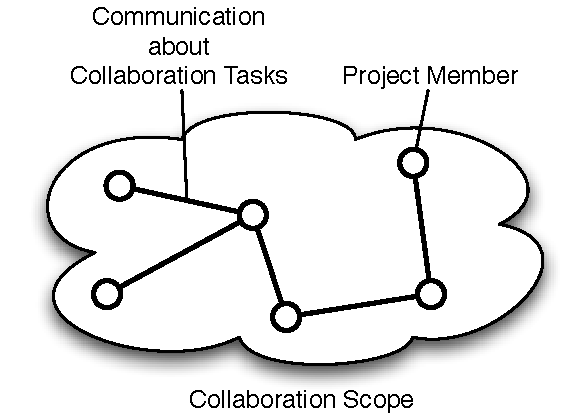
\includegraphics[width=8.0cm]{./figures/concepts}
% \label{fig:concept}
% \caption{Concept Visualization}
% \end{center}
% \end{figure}

\begin{figure*}[t!]
\begin{center}
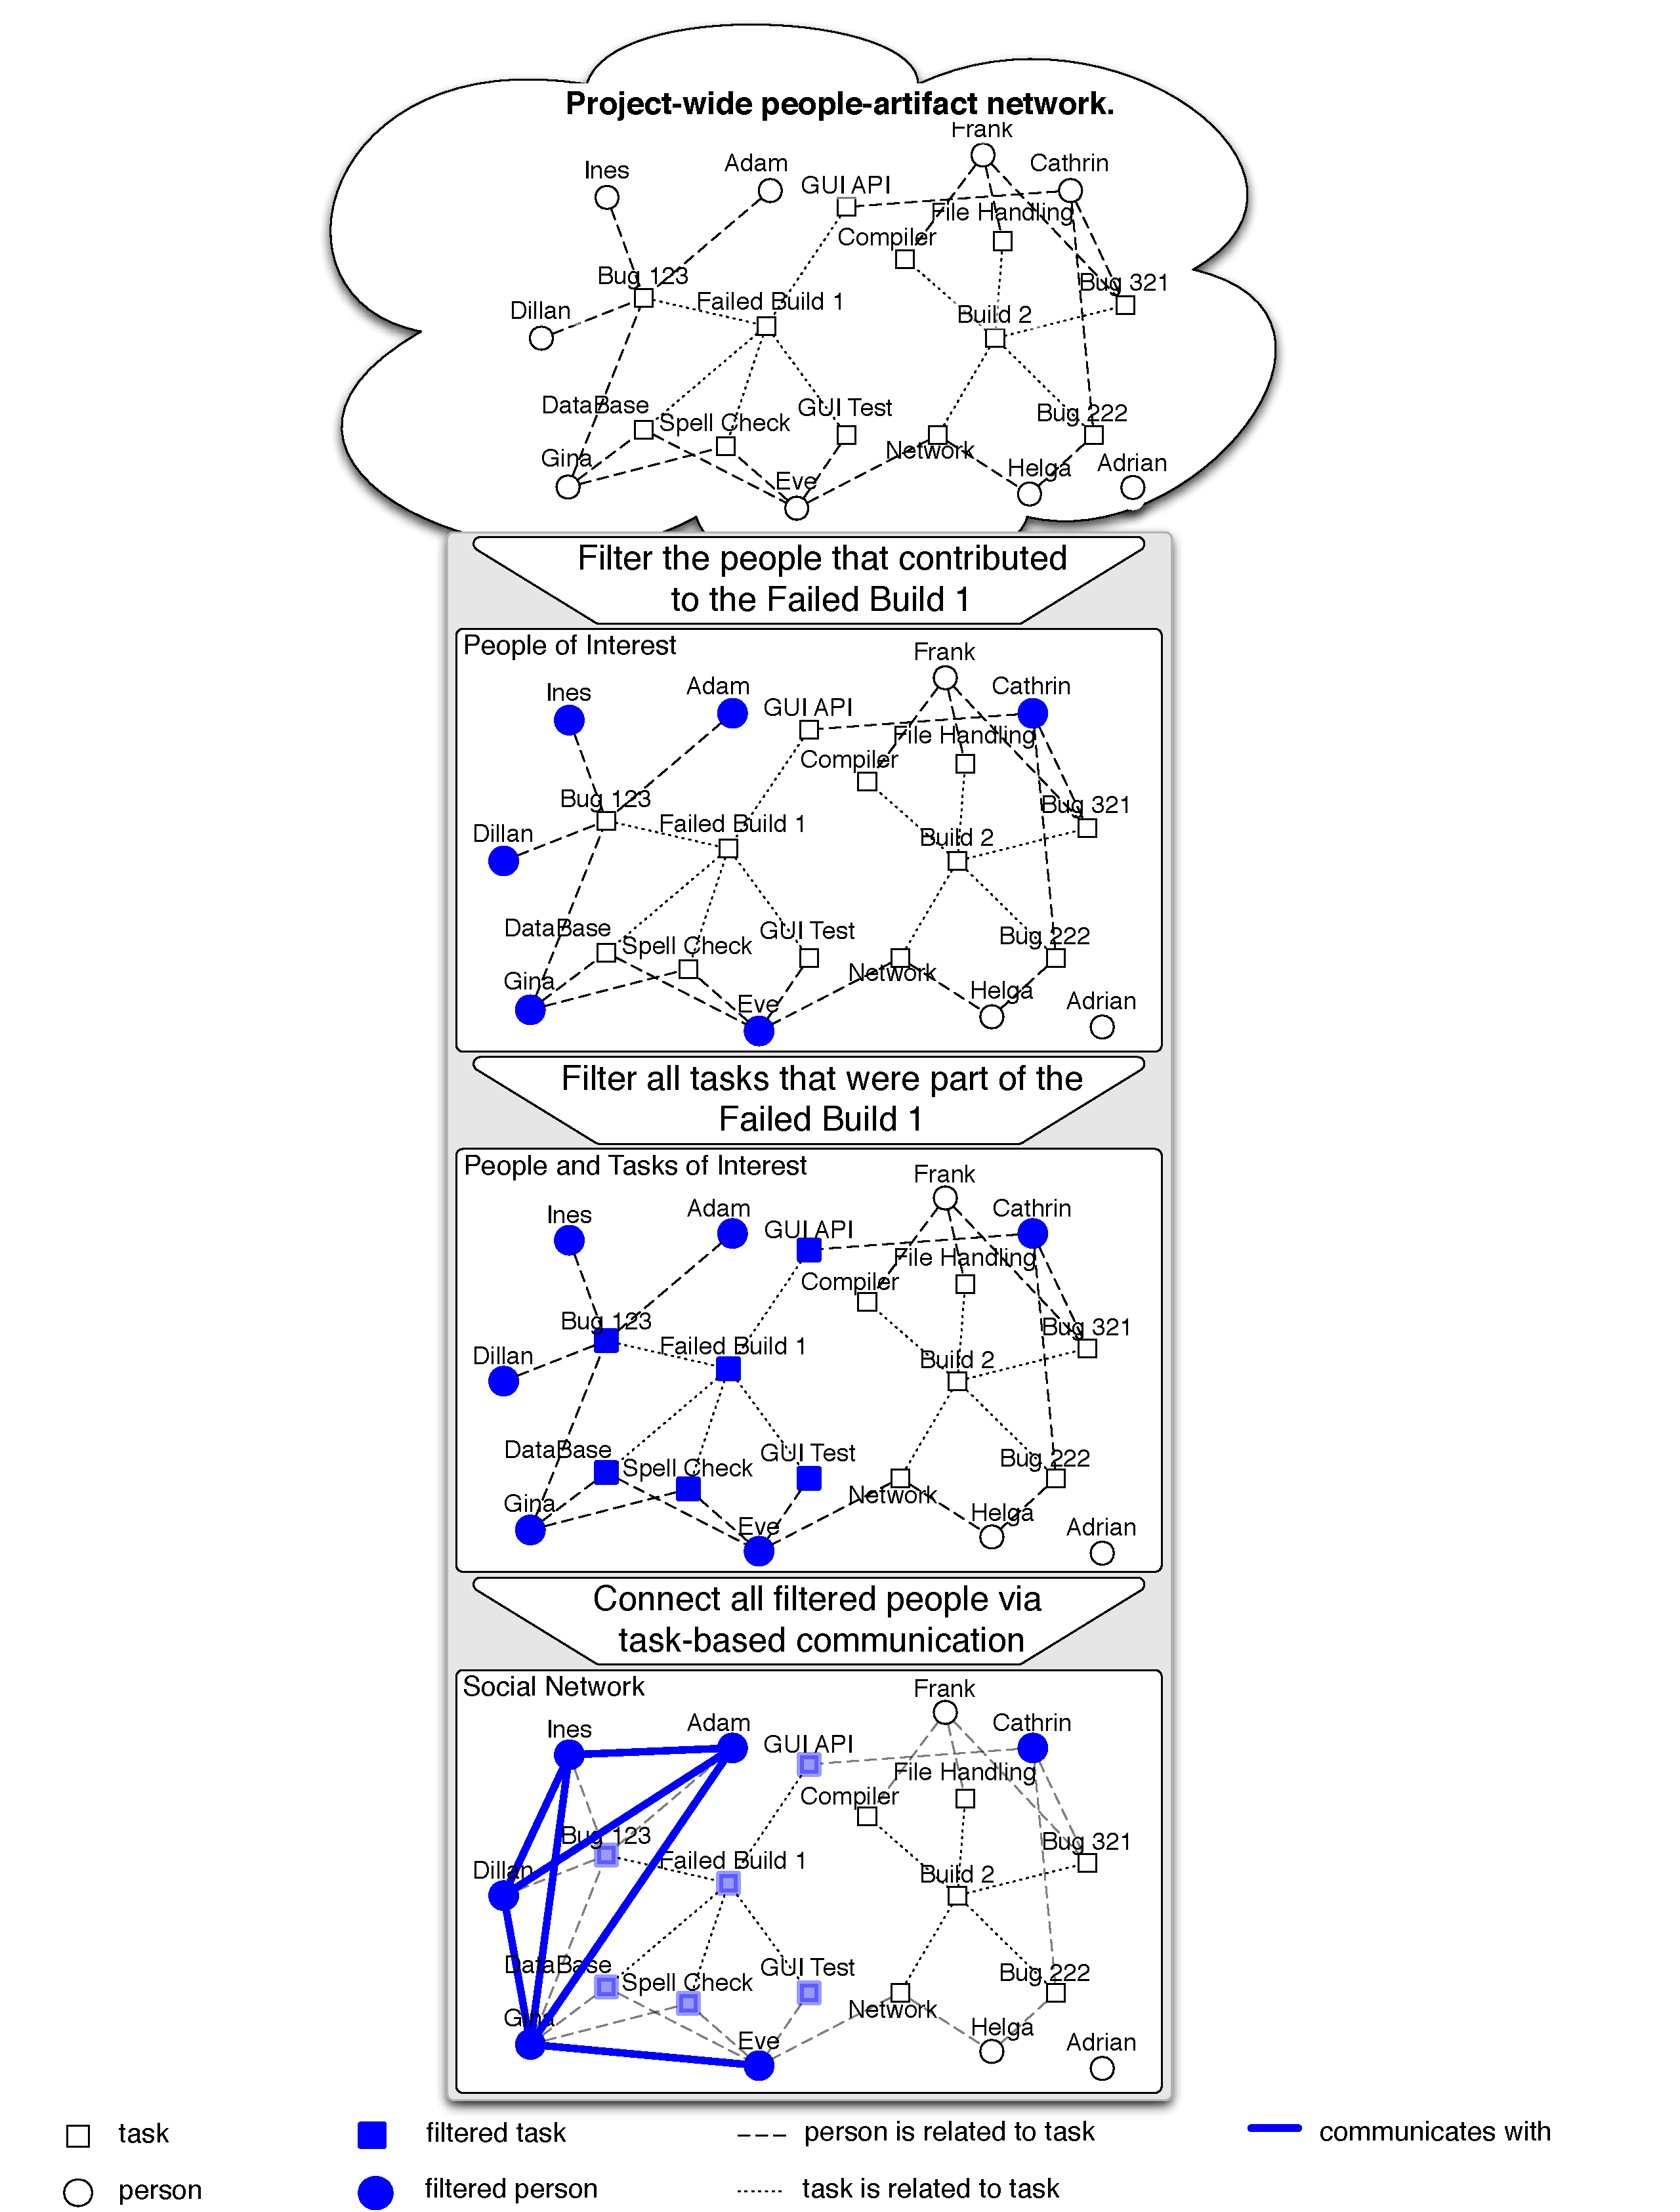
\includegraphics[height=0.9465\textheight]{./figures/grand_figure}
\caption{Social network construction examples in our approach}
\label{fig:network}
\end{center}
\end{figure*}

\subsection{Constructing Social Networks:}
The following three steps are used to construct a social network within a
collaboration scope: filtering of project members to identify nodes in the
network, filtering collaborative tasks to use as the context for collaboration,
and connecting project members to identify edges in the network. Each filtering
step includes criteria and reduces the set of \people s or \cu s from the entire
project. After collaborative tasks and team members are filtered, recorded
task-related communication is used to connect the nodes in the social network.

\paragraph{Filtering Project Members:}
To determine the set of nodes to be included in the social network we identify
those \people s that meet the criteria specified in the collaboration scope. In
our example, we restrict the team members to those who contributed to the failed
build, such as Adam, Eve, and Cathrin (coloured blue in Figure
\ref{fig:JazzProjectSN}). In addition, other constraints, such as temporal
% R2.1
constraints on when team members communicated about a task, can be added to
further reduce the included set of \people s.

\paragraph{Filtering Collaborative Tasks:}
Similar to the filtering of \people s, we use the criteria from the collaboration
scope to select \cu s. The \cu s provide the communication context used to
connect \people s in the following step. In our example, we restrict the tasks to
those included in Failed Build 1, such as GUI API, Bug 123, and GUI Test. The
filtering criteria can be based on properties of \cu s, such as task priority or
assigned team. Again, temporal constraints are often useful criteria, such as
selecting all development tasks contributed since the last build.

\paragraph{Connecting Project Members}
To connect \people s, creating edges in the social network, we leverage recorded
communication between the \people s in the filtered \cu s. For example, Gina and
Ines have both commented on Bug 123 and so we create an edge between them in the
social network. Our approach to constructing task-based social networks also
enables the inclusion of directed and weighted edges. Directed edges can
represent the direction of communication such as email sent from one team member
to another. Weighted edges can be used to represent the volume of communication
such as the number of emails sent.

\paragraph{}
While the filtering steps are independent, the order in which they are applied
can affect the composition of nodes and edges in the resulting social network.

\subsection{A Second Example -- Communication Brokers}
Here we provide a second example, applying project member and task filters in a
different order with differing criteria. This example demonstrates how social
networks can be used to find communication brokers between two project members.
This example is illustrated in the right column of Figure \ref{fig:network}.

Suppose, again, that you are the manager of a software team. Helga, a developer
in your project, complains that she needs information from Adam, but Adam has not
responded to information requests. Helga needs this information to complete her
work on Bug 222. You suspect that, due to time zone differences between
offices, Helga and Adam are rarely working at the same time and have trouble
communicating effectively. Social network analysis can identify other people in
the project that may be able to broker communication between Helga and Adam.

To construct a social network for this application, we filter the collaborative
tasks in the project keeping all tasks (coloured green in the right column of
Figure \ref{fig:network}). Then we filter the project members, keeping those that
have contributed to those collaborative tasks. Finally, using the recorded
task-based communication, we connect the project members to create a social
network for the entire project. By visualizing this social network we see that
Gina and/or Eve are good candidates to broker communication between Helga and
Adam. Choosing to use either Gina or Eve as a communication broker could be done
based on their geographic location with respect to Adam.

\paragraph{}
These two examples illustrate how the same repository could be mined for two
different collaboration scopes of interest to construct two different social
networks. An overview of software repository mining approaches to generate
developer networks are outlined in the Constructing Developer Networks sidebar.




\begin{figure*}[t!]
\begin{center}
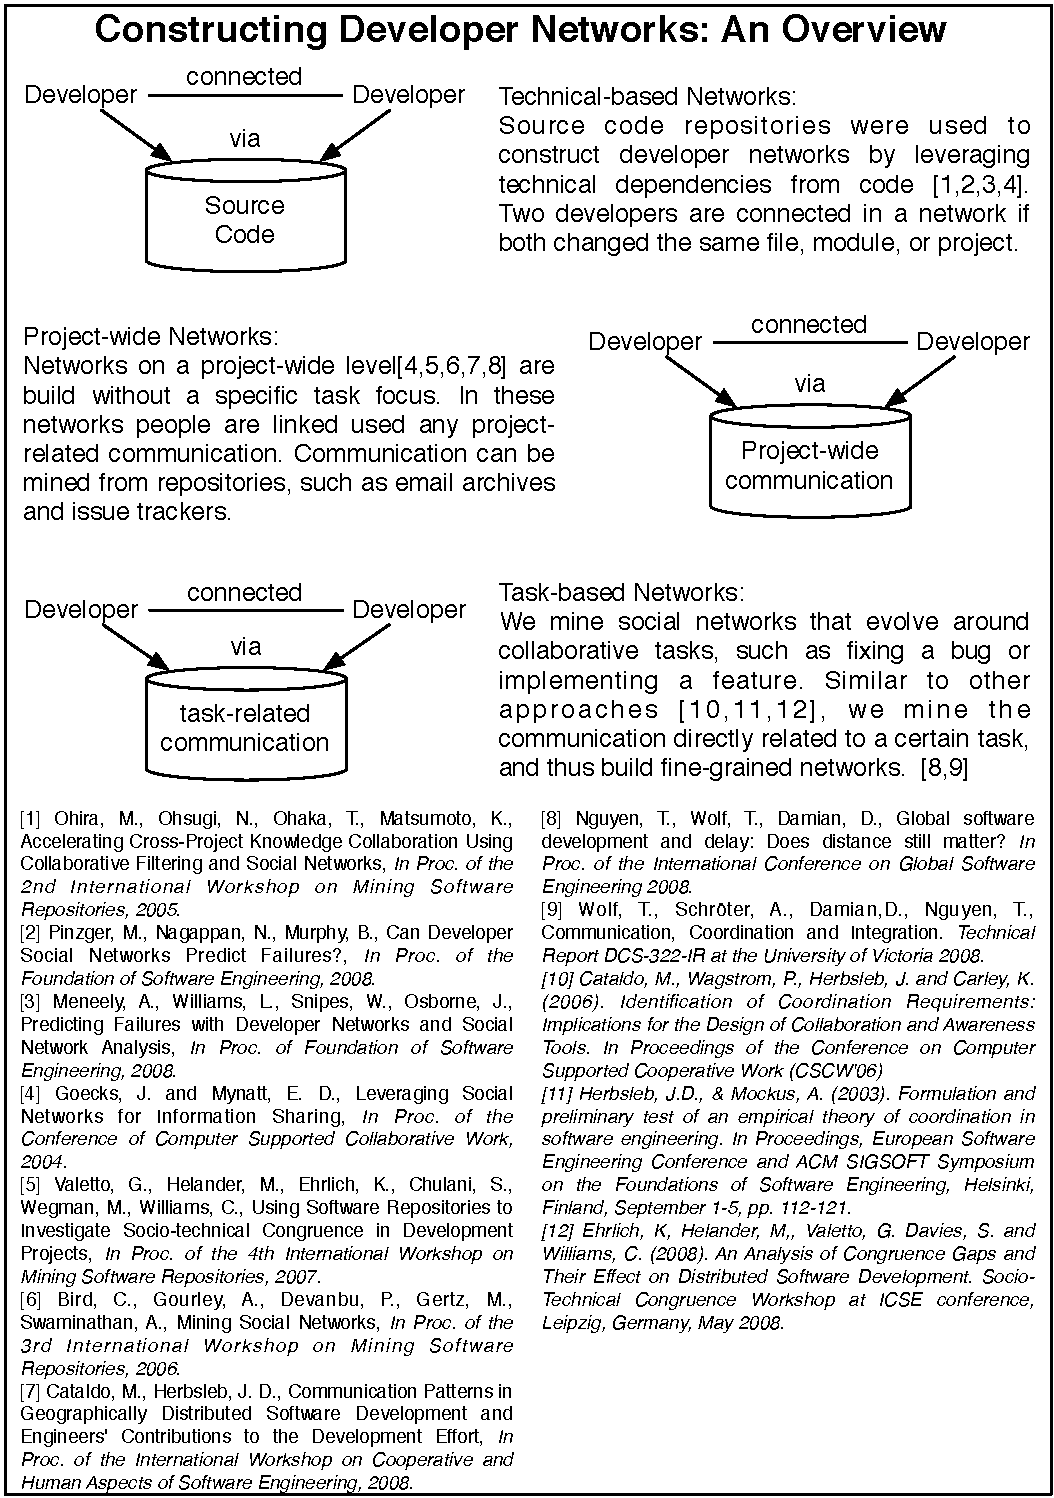
\includegraphics[width=0.7\textwidth]{figures/related_work.pdf}
%\caption{Constructing social networks}
%\label{fig:indep}
\end{center}
\end{figure*}



%[Some intro of Jazz repository]

% Commenting on work items is the main task-related communication and collaboration
% channel used by \jazztm\ developers. Work items represent single
% assignable and traceable tasks and a set of work items defines the tasks for each
% team in each iteration. Different types of work items represent defects,
% enhancements, user stories, and general tasks. The work items are assigned to,
% and owned by, project participants. The coordination that is necessary for the
% implementation of the work items is facilitated by work item collaboration
% behavior that includes contributors to comment or observe the communication
% around work items, by being subscribers to the work item.

\section{Social Network Analysis with \jazztm}

We applied our approach to mine and construct social networks with the IBM
Rational \jazztm\ project in several research studies. First, we describe how
\jazztm\ concepts and artifacts were mapped to the concepts used in our general
approach. Then, we describe our data mining tools, followed by two research
studies conducted using data extracted from the \jazztm\ development project.

IBM Rational is building \jazztm\ \cite{frost:ieeesoftware:2007} as a scalable and
extensible team collaboration platform for integrating development work across
task, build, source code, and planning management activities. \jazztm\ is
developed by a globally distributed team that uses \jazztm\ to manage its own
work. The \jazztm\ platform uses a client-server architecture, where the server
is the central data repository that stores data for \jazztm\ components. The
repository is accessible using a web-based client interface or an Eclipse-based
client. Our elements for constructing social network map to Jazz artifacts as
follows:

\begin{description}
\item[Project Members] are \emph{contributors} in Jazz.
Personal information, such as the name and email address of each contributor, as well as
project related information, such as team affiliations are available.

\item[Collaborative Tasks] are \emph{work items} in Jazz. Work items represent
the basic unit of work in \jazztm\ and can describe many types of tasks such as
bug reports, modification requests, or development tasks. Work items have a
comment-based conversation, a list of observing subscribers, and other attributes
such as, a creation date, a description, and an owner.

\item[Task-related Communication] is \emph{comments} on work items in Jazz.
Reading and writing comments on work items is the main collaboration mechanism in
Jazz as developers use comments to debate and discuss decisions. A thread of
comments forms a conversation that is attached the work item. Each comment
has a creation date, comment text, and an authoring contributor.

\end{description}

% XXX -- fix my location
\begin{figure*}[tb]
\begin{center}
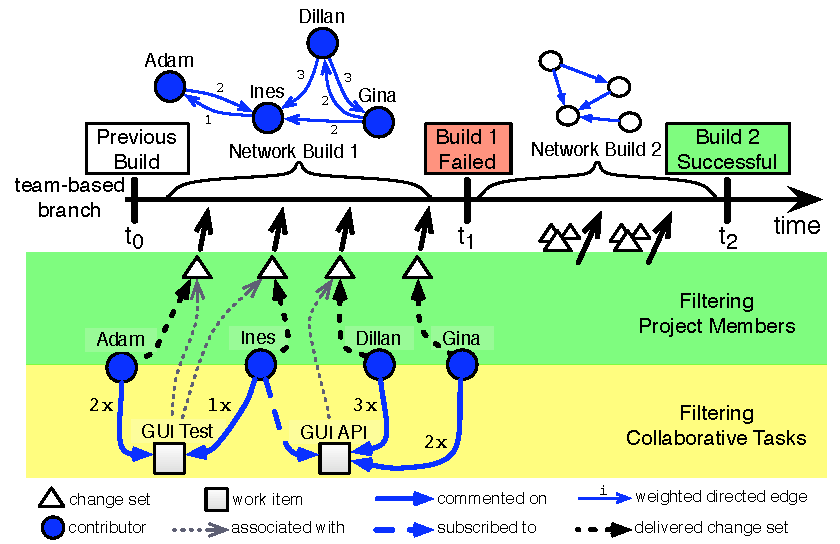
\includegraphics[width=1.3\columnwidth]{./figures/BuildResultNetworks}
\caption{Construction of social networks for build failure prediction}
\label{fig:BuildSNs}
\end{center}
\end{figure*}

\subsection{Data Mining Tools for \jazztm}
In order to extract the elements needed to construct and analyze social networks,
we implemented several data mining and social network analysis tools. To extract
data of interest, we developed a plug-in for the Eclipse-based \jazztm\ client
that used the provided Java API to query and retrieve the desired data from the
repository.

The \jazztm\ development project has a large \jazztm-based repository containing
more than 40,000 work items, 150 contributors, and 5,000 build results. We
needed to collect data from the live development repository without affecting the
\jazztm\ development team's server performance, potentially disrupting their
work. To meet this goal, we designed our data extraction tool to be minimally
invasive and to use incremental queries, extracting small portions of the data
set at a time, to minimize performance degradation.

Further, the querying and processing of the extracted data to construct social
networks is an additional challenge because it is data and time intensive. For
example, extracting and processing all work items from the repository took
several hours. Thus, it is not feasible to extract and process all of the
information needed to construct social networks in real-time. For this reason, we
import the data of interest into a reporting and analysis database. This approach
allowed us to use a large proportion of the data in the \jazztm\ team's
repository for social network construction and analysis without adversely
affecting their development environment.

% Each data type's external XML file representation is independent so that a single
% query result can already be used for analysis, without requiring all associated
% data types or associations. For example, when only exporting the work items that
% were created or modified during a specific week, the resulting data file can
% already be analysed without the need of any associated data types like the
% contributors. In addition, data and associations between data types that result
% from subsequent queries can be added without changing the previous extracted
% information. This data structure enables us to mine large data sets in many small
% through incremental queries without affecting the Jazz server repository.

To process the data from the database we used the Java Universal Network/Graph
Framework (JUNG) to construct and visualize the task-based social networks and to
compute social network analysis measures. Our tools also generate data sets for
use as inputs to other tools, such as statistical analysis using the R language,
or social network analysis using UCINET.

%\paragraph{Filter Project Members}
%\ \\
%In \jazztm\ we filter \people s by different criteria to focus on people to meet
%each collaboration scope. One way to do that would be to focus on all people that
%made changes to the source code included in a build. For that we would identify
%all chances made for that build and identify the people that made those changes.

%\paragraph{Filter Collaboration Tasks}
%\ \\
%One major task during the \jazztm\ development would be to deliver a successful
%build of \jazztm. Our XXX would focus on a build within \jazztm\ and only include
%work items that are build related. In addition, the XXX would define the time
%frame starting on the previous build and the build of interest.

%\paragraph{Connect Project Members}
%\ \\
%Contributors comment on work items to ask questions, debate descisions, or to
%provide additional information, such as screenshots. A series of comments on a
%work item forms a conversation thread. When connecting \people s while
%constructing our social networks, we connect those who have commented on a work
%item, as we assume that they have exchanged information and thus communicated.
%Additionally, we assume that subscribers of a work item listen to the
%communication, but have not actively contributed. We also include the creator of
%the work item as a contributor because a work item's initial description is the
%start of the conversation.

% The communication between two \people s is directed, since participating in a
% work item conversation thread means sending and receiving information. Whereas,
% subscribing to a work item only provides one-way communication, so directed edges
% are used to connect \people s. Weights can also be applied to communication links
%  by using the number of comments exchanged between two \people.


\subsection{Research Studies Using Social Network Analysis}
We used the mined task-based social networks in two of our research studies that
map to the more general build failure \cite{wolf:tr2008} and communication
broker \cite{Nguyen:2008Distance} examples provided earlier.

\paragraph{Communication Structures to Predict Build Failures}
\ \\
In this study we were interested in investigating whether properties of an
integration team's social network have any relationship with the integration
outcome. Code integrations (referred  to  as builds in Jazz)  are frequent and
very important in the Jazz project. The continuous integration process requires
regular daily and weekly integrations of each team's work into an assembled
product. A build can succeed or fail due to compilation, testing, or other
integration errors.

To integrate in \jazztm, the members of a development team commit source code
changes (change sets) to a team-based branch. Each change set is associated with
the work item that describes the change it implements, and contributors comment
on the work items to discuss the changes. As such, the \emph{collaboration scope}
of this study is the communication of contributors who have delivered change sets
that were included in each build. 

%DD. Shortened the text to avoid repeition from section 1, as per comment #2

To construct the social networks for Build 1 at time t$_1$ (as illustrated in
Figure~\ref{fig:BuildSNs}), we followed the steps outlined in our Failed Build
example described earlier: we filtered the contributors that delivered change
sets between t$_0$ and t$_1$ and identified all work items that were associated
with code change sets in Build 1. To connect contributors in the social network
we add a directed edge between each pair of contributors who have either
commented or subscribed to a common work item since the last build. The weight on
directed edges represents the number of comments on the shared work items.

% T.W. Changed the following paragraph to address point 3 from revision 2
After we constructed the social networks for each integration build of the five
teams
% R3.2
(between 48 and 60 builds for each team), we computed different social network
measurements, such as \emph{centrality}, \emph{betweenness}, and
\emph{density}~\cite{Wasserman:1994dz} and investigated their relationship to
integration outcomes. Although none of these measures can independently predict
the build outcome, when used in combination they are more powerful. We developed
a predictive model by training a
% R2.4
Bayesian classifier that was able to accurately predict failed build results. The
recall and precision values of the predictions using measures of social network
structure is shown in Table~\ref{tab:predictionResults} for the five teams.
% R3.2
In order to validate our model for each of the five teams we used \emph{leave one
out cross validation}, which trains a model for each set of data points that is
in size one smaller then the full set, and then predicts the data point that is
not in the training set. Study details are available in technical
report~\cite{wolf:tr2008}.


\begin{table}
\small
\begin{tabular}{r|c c c c c|c}
\hline
  & \multicolumn{5}{c|}{Teams} & Std.Dev. \\ \hline
Recall 		& 55\% & 75\% & 62\% & 66\% & 74\% & 8.38\% \\ 
Precision 	& 52\% & 50\% & 75\% & 76\% & 66\% & 1.34\% \\ \hline
\end{tabular}
\caption{Prediction results for the five teams}
\label{tab:predictionResults}
\end{table}



% R2.4 NOTE FROM DANA: NO NEED TO HAVE THIS NEXT PARA, SO I COMMENTED IT. THE
% REVIEWER WAS JUST BEING VERY TOUGH.. 
% Although, the results are compared to a general failure probability of 50\%, we
% consider this result as a first step towards indicating that communication
% influence source code quality.


\paragraph{Communication Structures in a Large Distributed Project}
\ \\
In this second study \cite{Nguyen:2008Distance} we were interested in the
project-wide communication structure of the geographically distributed \jazztm\
development team. A quantitative analysis of response time for task
communication and task resolution times revealed a lower than expected impact of distance on these
factors. We explored the project's social networks for useful insights that might
explain this effect. Specifically, we were interested in identifying properties
of the social networks, such as cohesiveness of the distributed teams, that were
related to the results of communication delay and distributed collaboration.

The \emph{collaboration scope} of this study is the entire project, and thus
includes all collaborative tasks, and all contributing project members. In this
case, connecting project members is the key step to create a project-wide social
network. 

%DD shortened the text to address comment #2. 
To construct the project-wide social network we followed the steps as
exemplified in Section 1.3 (the communication broker example).


The resulting social network is illustrated in Figure~\ref{fig:JazzProjectSN} in
which ovals indicate the teams at each geographic site. We used the \emph{k-core}
and \emph{core-periphery} tests \cite{Wasserman:1994dz} to analyze the properties
of the network structure. These tests allowed us to test whether multiple
cores can be identified in the network, or the network shows a star-like 
structure in which a single core mediates communication with the developers on
the periphery of the network.
%R3.5 && R2.5

The results indicate that the project-wide team collaborates as a cohesive team
with one large core, as opposed to many loosely connected clusters. The colors in
the figure illustrate how close a team member is to the core of the whole
project. In red we show a core of active developers (60 of
112 project members) where each developer
communicates with at least other 25 developers from the core. The other
colors, from yellow to light blue, indicate different lower degrees of communication in
the project. Further, using the
\emph{group degree centrality} \cite{Wasserman:1994dz} measure, we also found
that each geographic location has roughly equal centrality and used the people in
the core to stay connected to the rest of the large team. This means that project
members communicate well with project members at each other geographic location.
This may explain why distance had an insignificant effect on communication response
and task resolution time in the large distributed team.

% R3.2
In summary, we learned from this study that communication delay as a result of
distribution in global teams can be overcome with recent
collaboration tools and practices. From our experience with the Jazz team, best practices such as prioritizing
off site requests and tools that integrate development, project
management and communication play a major role in achieving these results.

\begin{figure}[t]
\begin{center}
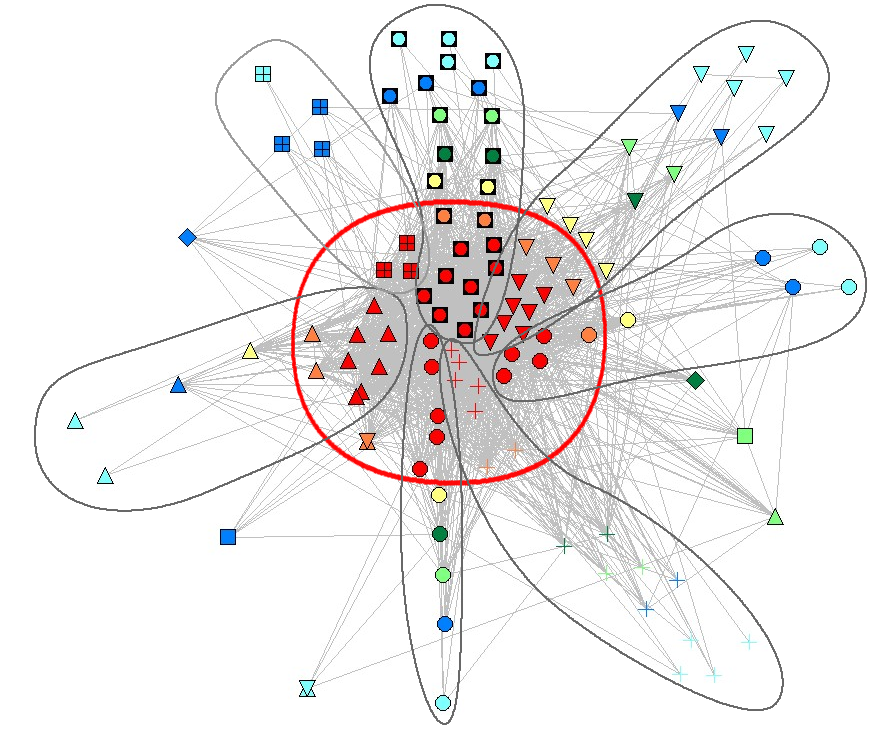
\includegraphics[width=0.99\columnwidth]{./figures/JazzProjectSN}
\caption{Project-wide communication-based social network}
\label{fig:JazzProjectSN}
\end{center}
\end{figure}

% ~\cite{Seidman:1983sn}
 % ~\cite{Borgatti:2000kl}
% ~\cite{Everett:2005dn} Details are published






\section{Practical Implications for Deployment} 
% [How to integrated our approach in the used repositories and tools to support
% project during development?]

Our approach to mining and constructing social networks, as well as the results
of our studies, have several implications for software practitioners.

\paragraph{Scalable Mining and Analysis Tools}
\ \\
By incrementally mining and using a secondary reporting database (or data
warehouse), we can reduce load and performance problems on the mined software
repositories. Our approach is useful for practitioners who must not impact the
performance of their team's repositories.
% R3.3
This has been proven useful during our extraction of information from the Jazz
repository, which was under constant load due to the global distribution of the
more than 140 Jazz team members.
%
Extracted data, constructed networks, and network analysis measures can be stored
in the data warehouse to avoid extracting or recomputing them multiple times. For
example, the social network using the set of work items and communication around
each build can be stored in the data warehouse and is directly accessible for any
number of further analyses. Computationally intensive analysis and predictions
can be conducted using the data warehouse or by a client accessing the data
warehouse. Once task-based social networks and network analysis measures are
stored in a data warehouse, visualization of social networks and further analysis
becomes efficient and non-intrusive to the users of repositories.

% These networks and measures can assist developers, enabling task-awareness and
% expertise seeking. Additionally, team-leaders and managers can examine social networks and their computed measures
% in the context of project performance data such as integration outcomes.

\paragraph{Team Awareness through Social Network Visualization}
% \ \\ 
Developers working on interdependent tasks can benefit from the visualization of
the social network of the team members who contributed to the interdependent
tasks. The information in the network can include developer contact and
availability, as well as a list of other tasks that they are working on. This
information is particularly important for newcomers to a project, who lack
project specific expertise, such as who has been involved with a particular task,
or in architectural decisions.
% R3.3
We are currently conducting a case study to identify which information is
valuable to support developers and what visualization conveys them most
effectively.
 



% Collaboration scope  focusing on specific teams, inter-team communication, or
% specific task criteria.

\paragraph{Outcome Prediction Using Social Network Analysis}
\ \\
Another application for social network analysis is to predict project outcomes
such as build results based on information about team communication behaviour.
Practitioners can build tools that are embedded in the development environment
that inform developers about the health of upcoming builds. An awareness
notification system that uses a build failure prediction model could indicate
whether the current communication patterns are likely to result in a failed build. 

Building a predictive model from social networks constructed with data mined
from task and task-communication repositories could be done with the following
four steps:

% Note that the steps focus on the integration builds a a certain team and can be
% applied for all teams in parallel.

%\begin{enumerate}

%\item In frequent time intervals (e.g. 30 min.), the social network is
%constructed on the communication about the tasks that are associated with the
%source code changes that are made after the last build. The construction requires
%the querying of the main repositories. The social network measures are computed
%for the network and the resulting measurements and the network are stored and cached in
%the warehouse so that the subsequent network constructions only need to query the
%communication data from the last time interval (e.g. 30 min.).

%\item The trained predictive model that is stored in the warehouse and the
%computed network measurements are used to predict the result of the next upcoming
%build. The prediction result in the warehouse is accessed by the development
%environments to indicate the current prediction result to the developers.

%\item Whenever an integration build finished, an automated process queries the
%remaining new communication that occurred after the last network construction
%from step 2 and the time of the build. The final build related
%communication-based social network and its measurements are constructed, computed
%and stored in the warehouse. The process can either be triggered by notifications
%on subscription or by frequent look-ups.

%\item A new prediction model is trained on all build related networks and
%measurements that are stored in the warehouse. The trained model is stored in the
%warehouse and replaces the previously stored model. The data set that is used to
%train the prediction model increases with each new build and the predictions
%become more precise.
% 
%\end{enumerate}

% To build a predictive one needs to mine the social networks for each build in
% order to populate the data warehouse. All mined social networks of past builds and the associated
% build results are used to train a predictive model. Whereas the social network
% for the upcoming build is only stored in the warehouse for later predictions. 



\begin{enumerate}
\item \textbf{Initialization Predictive Models:}
Initialize the predictive model using the social networks and
outcomes for all existing builds. Store the data on social networks, build
outcomes, and predictive model in a data warehouse for later use.
\item \textbf{Construct Social Network for Upcoming Build:}
Construct the social network for the upcoming build as described
in our approach.
\item \textbf{Predict the Upcoming Build Outcome:}
Calculate network analysis measures for the constructed social
network and use them as input to the predictive model. The model then predicts
an outcome for the upcoming build. At this point, a manager could make
proactive adjustments to attempt to prevent a predicted build failure.
\item \textbf{Update Predictive Model:}
Finally, after the upcoming build has been completed, update the predictive
model to include the social network, network measures, and outcome of the latest
build. The model can then be used again to make an outcome prediction for the
next upcoming build (starting with Step 2).
\end{enumerate}

% Note that steps 2 and 3 are executed repeatedly and only interrupted when a build
% is done in step 4.

%This repository mining and model building approach using task-based
%communication can also be applied to predicting other project-related variables
% such as post-release defects or iteration scheduling accuracy.

If the system indicates a build failure, further analysis could
identify communication deficiencies and prompt managers to rectify the problem
before the build occurs, as described next.
% R3.3
% We are currently conducting a case study to identify how the predictions are
% used by the Jazz team.


\paragraph{Effective Management through Social Network Analysis}
% \ \\

%R0 and R2.6
Beyond visualizations, computed social network measures can be used
by
management as an aid in preventing failed builds. Our research shows that the quality of
communication does matter in the quality of integrations. Monitoring and
affecting communication behavior is a strategy to prevent failures. Software
engineers differ in the expertise and knowledge they bring to collaborative tasks. Team
performance depends not only the information available to developers and the
distribution of knowledge within the team, but also on the communication
structure that facilitates knowledge dissemination within the team. Although we
have no evidence that individual measures of communication structure can
predict integration failure, these measures can be used in identifying
problematic communication behavior likely to result in failed integrations.
Actions that management can take to prevent failures for a
particular team include:

\begin{enumerate}
\item \textbf{Compute Social Network measures or Run Predictive Model early in
the project:} In our study of Jazz, the predictive model performed well even
with the first 25\% of the team communication data (i.e. first quarter of
project timeline). If this is true in other development environments,
practitioners should use this information very early in the project. If the
model predicts error, see next step. Otherwise, computing social network measures such as
density, betweeness and centrality early in the project is an alternative
option that could signal problematic communication behavior in the project.
\item \textbf{Examine team communication structure:}
Identify the presence of patterns of communication that can, when analyzed in
light of project specific technical dependencies, be problematic. An example of
problematic communication structure indicated by social network
measures is that of a team with high coordination needs before an integration
but with a communication network of low density. It is possible that there are too many missing communication links between developers that have
technical dependencies~\cite{ehrlich2008:gaps}, or
there is an overall lack of communication in the team. Another example is of a team with several
distributed subteams that need to coordinate and in which a number of
developers have high betweeness but the subteams themselves have little
communication across distance. This may indicate that there are
clusters of developers who should communicate directly, and that
the subteams are only loosely connected and have communication brokers that
may become bottlenecks. 
\item \textbf{Improve communication or knowledge management
procedures:} Adjust communication and knowledge management processes or tools in
the project, to address specific situations identified at previous step. 
If communication links between developers with
coordination needs are missing, assigning communication brokers so that
these developers can better coordinate interdependent work is an
option. Equally valuable, increasing the awareness of these coordination needs
as well as developers' expertise areas in the current project could be done
through regular project meetings or more adequate documentation of these dependencies in project specific knowledge repositories. In other situations, if
communication across distances is relying on information brokers, managers
should consider supporting alternate points of contact in the clusters
identified as relying on these brokers, or enforce documentation of information
that becomes available to everyone in the project. Both these options help
mitigate the risk of information brokers becoming unavailable in the project. 
\end{enumerate}

Despite our intention to be as specific as possible, these 
recommendations for action should consider and be applied in the
particular context of each project. Managers should use the
insights obtained from the examination of communication structures in their
project as a starting point in their further analysis of 
communication in relation to the particular technical and
organizational characteristics of their project.




% Using social network measures, one can
% detect the presence of communication clusters in a distributed project, or
% dysfunctional behavior, such as a lack of communication activity around a
% critical task for an upcoming release.

% On a regular basis, the measures can be reported automatically for the
% project-wide communication network or for specific collaboration scopes. For
% example, this focus can be on tasks related to specific activities (e.g.,
% requirements analysis or maintenance), or certain task properties (e.g., tasks
% within a time range, with high priority, or assigned to one team). Managers and
% team leads monitoring these reports can then maintain awareness of the
% communication structures and possible sources of communication problems within
% these contexts. Detecting problematic communication structures, such as loosely
% connected teams where brokers may become bottlenecks enables project leaders to
% take action and adjust communication processes in a timely and proactive manner.




% \section{Related Work} The related work consists of three parts. The first is
% focused on how social network were build in the past. The second shows practical
% applications that make use of social networks and the third part gives a quick
% overview over  what has been done with regards to failure prediction.
% 
% \subsection{How To Build Social Networks} Most automatically constructed social
% networks are mined from SCM's~\cite{msr07:weissgerber,msr04:lopez,fse08:pinziger,
% fse08:meneely}. These approaches usually assume that two
% developers that worked together on a module are connected. In this case working
% means that they changed the same module within a pre defined timeframe. This has
% of course the disadvantage that the project specific communication between
% developers is missing. One way to capture part of this communication is to mine
% e-mail archives~\cite{bird:msr:2006,fse08:bird}. Still this medium is incomplete with
% respect to actual ongoing communication therefore we leverage the discussion
% around work items as provided within \jazztm\. But where were such social networks
% used?
% 
% \subsection{Practical Applications for Social Networks} Social network have been
% used in many different ways. Recent research has manly focused on knowledge
% distribution and failure prediction.
% \begin{description}
% \item[Knowledge.] Efficiently distributing knowledge and fostering awareness in
% teams is a hot topic within software development.
% Several studies have addressed this issue recently. They reach from expertise
% recommending systems within \cite{msr07:minto} and across projects \cite{msr05:ohira}.
% \item[Prediction.] Other studies have leveraged simple networks mined from SCM's
% to predict the existence of post release failures in software modules like
% binaries~\cite{fse08:pinziger,fse08:meneely}.
% \end{description}
% Of course there are more than these application like ... argued the congruence of
% social and technical networks is of use for It governance and de Souza used
% social networks to study the behavior of teams with respect to whom they need and
% want to display their actions.
% 
% \subsection{Failure Predictions} Recent research mostly focused on predicting
% whether a software module (e.g. files or binaries) will fail after shipping a
% product. Most features used to predict this kind of failures leverages the
% technical part like module dependencies, code changes or simply code complexity.
% One of the more recent prediction models by Zimmermann and Nagappan uses social
% network measures on module dependency graphs to predict if a module is
% failure-prone~\cite{icse08:zimmermann}. Others leveraged organizational structures
% evolved around software modules. They connected those modules via developers that
% worked on them to the organizational structure~\cite{icse08:nagappan}. There have been
% studies that go one step further and do not focus on organizational structures
% but look at how developers are connected, mainly those studies like ... and ...
% constructed their networks from SCM systems. These networks connect developers
% through modules they worked on together, which of course misses every other
% communication that went on during that time.
% 
% All in all those approaches focus on failures that will occur after the release
% of a software product since those are most inconvenient for the end user. In
% contrast to that we focus on the product quality during the development. In
% particular on the outcome of builds since if your build does not satisfies the
% minimum quality requirements or does not even build than you cannot ship the
% product. Kim et al. had a similar approach which is more fine grained. They
% predicted if a change introduces a failure into the software \cite{icse07:kim}. This
% method can be used during development but the fine level of detail does not focus
% on the important part namely predicting if you reached a deployable state or not.




\section{Conclusions}
Task-based social network mining and analysis enables you, as a participant in a
software project, to tap into a vast pool of otherwise inaccessible communication
information. Our approach has been applied to two scenarios with the Jazz project
illustrating its applicability and gleaning new insights into the social patterns
of that team. The use of social networks in software engineering is relatively
unexplored and holds much promise for future applications.

%  Mining repositories and social networks gained focus by researchers to analyze
% software development projects and the involved technical and human
% relationships. While researchers published impressive findings, few of the
% techniques are integrated and used in the development environment to directly
% support the project. We provide an approach of mining task-related
% communication-based social networks for any repositories that support \people
% s, \cu s, and communication. The feasibility of the approach is shown by two
% studies mining the Jazz repository of the Jazz development project. We propose
% to utilize social network analysis to directly support the mined project. A
% variety of practical applications in the area of reporting or awareness
% applications can support the daily work of project participants by integrating
% the mining process into the development environment. We propose initial steps
% to realize the integration without affecting the performance of the main
% repositories used.


%%%%%%%%%%%%%%%%%%%%%%%%%%%%%%%%%%%%%%%%%%%%%%%%%%%
%%%%%%%%%%%%%%%%%%%%%%%%%%%%%%%%%%%%%%%%%%%%%%%%%%%
%%%%%%%%%%%%%%%%%%%%%%%%%%%%%%%%%%%%%%%%%%%%%%%%%%%
%%%%%%%%%%%%%%%%%%%%%%%%%%%%%%%%%%%%%%%%%%%%%%%%%%%
%%%%%%%%%%%%%%%%%%%%%%%%%%%%%%%%%%%%%%%%%%%%%%%%%%%

\startchapter{Technical Relations and Failure}


%%%%%%%%%%%%%%%%%%%%%%%%%%%%%%%%%%%%%%%%%%%%%%%%%%%
%%%%%%%%%%%%%%%%%%%%%%%%%%%%%%%%%%%%%%%%%%%%%%%%%%%
%%%%%%%%%%%%%%%%%%%%%%%%%%%%%%%%%%%%%%%%%%%%%%%%%%%
%%%%%%%%%%%%%%%%%%%%%%%%%%%%%%%%%%%%%%%%%%%%%%%%%%%
%%%%%%%%%%%%%%%%%%%%%%%%%%%%%%%%%%%%%%%%%%%%%%%%%%%

\startchapter{Communication and Failure}
Communication problems lead to coordination and integration failures in work
teams (e.g.~\cite{Grinter:1999geography,Herbsleb:1999ew,souza:cscw:2004}). This
situation is further exacerbated in large and distributed teams, where effective
communication and activity awareness of related but remote project members are
problematic, yet key to anticipate and resolve coordination problems early
(e.g.~\cite{Grinter:1999geography,Herbsleb:1999ew}).

We strive to contribute to the growing body of research into the role of
communication structures in determining coordination ease~\cite{hinds:cscw:2006} and
success~\cite{hossain:cscw:2006}. Although there has been some research on the
relationship between communication and coordination in work teams, research in
software engineering is very limited. The study of the Enron email corpus found
that central communicators exhibit a better ability to
coordinate~\cite{hossain:cscw:2006} and R\&D teams with dense communication
structures are associated with more coordination problems~\cite{hinds:cscw:2006}. In
open source software development, developers that are active in email
communication have also been found to be most active in open source
development~\cite{bird:msr:2006}. In software engineering research, however it is
unclear whether there are specific communication behaviors that enable effective
coordination. Moreover, we are missing a precise conceptualization and objective
measure of what successful communication in relation to project success is.

Complementary to previous research that is largely qualitative
\cite{herbsleb2003:speed,Holmstrom:2006gd} and which gathered information about
occurrences of communication problems through project reviews and subjective
ratings of project success, we use objective measures in studying the
relationship between communication structures and coordination success. Past
research has also largely investigated communication and coordination only in
relation to entire projects. There is little systematic software engineering
research in objectively examining the outcome of coordination (successful or
failed) and assessing communication characteristics that lead to coordination
failures. In this work we investigate the relationship between communication
structures and coordination outcome at a finer level of detail. We study
instances of coordination during the integration of code in large and distributed
software teams, in relation to their associated communication structures. By
communication structure we refer to the topology of the communication network
that was involved in the tasks that lead to a software build. We use social
network analysis measures such as density and centrality to obtain measurable
characteristics of the communication structure.


Our study examines the data from IBM's distributed development project Jazz. Jazz
is a development environment that focuses on collaboration support and tightly
integrates programming, communication, and project
management~\cite{frost:ieeesoftware:2007}. Our two step study revealed the following: Our
results indicate that developer communication plays an important role in the
quality of software integrations. Although we found that no individual measure
could indicate whether a build will fail or succeed, we leveraged the combination
of communication structure measures into a predictive model that indicates
whether an integration will fail.

The remainder of the paper is structured as follows: we first discuss related
work (Section~\ref{sec:RelatedCommunication}) and introduce our two research
questions (Section~\ref{sec:ResearchQuestions}). Section~\ref{sec:Methodology}
describes our methodology in the study of communication structures and
integration in the Jazz project. Section~\ref{sec:AnalysisResults} describes the
results of our analysis. We close with their discussion and implications for
practice in Section~\ref{sec:discussion} and~\ref{sec:conclusion}.



\section{Communication, Coordination and Integration}
\label{sec:RelatedCommunication}

The relationship between communication, coordination and project outcome has been
studied for a long time in the area of computer-supported cooperative work. More
recently the domain of software and distributed software development showed
increased interest as well.

Communication plays an important role in work groups with high coordination needs
and the quality of communication has been found as determinant of project
success~\cite{curtis:acm:1988,kraut:1995coordination}. The dynamic nature
of work dependencies in software development makes collaboration highly
volatile~\cite{Cataldo:2007hb}, consequently affecting a teams ability to
effectively communicate and coordinate. Additional difficulties emerge in
distributed teams, where team membership and work dependencies become even more
invisible~\cite{damian:icgse:2007}. Moreover, team communication patterns are
significantly affected by distance~\cite{hinds:cscw:2006}. Maintaining
awareness~\cite{sarma:2006icgse} becomes even more difficult when developers work
in geographically remote environments; communication structures that include key
contact people at each site are effective coordination strategies when
maintaining personal cross-site relationships is challenging~\cite{hinds:cscw:2006}.

With respect to the role of effective coordination in project success, early
studies indicate the issues that software development teams face in large
projects~\cite{curtis:acm:1988}. A study by Herbsleb et
al.~\cite{Herbsleb:1999ew} showed that Conway's law is also applicable for the
coordination within development teams, supporting the influence of coordination
on software projects. Kraut et al.~\cite{kraut:1995coordination} showed that
software projects are greatly influenced by the quality of coordination of
development teams. More recently a theory of coordination has been proposed and
accounts for the influence of coordination on different project metrics such as
rework and defects~\cite{Herbsleb:2006vn}.


The importance of communication in successful coordination is also well
documented and makes the study of communication structures important. For
example, Fussell et al.~\cite{fussell:cscw:1998} found that communication amount and
tactics were linked to the ability of effectively coordinate in work groups. In
software development, others showed that communication problems lead to problems
during the activity of subsystem
integration~\cite{Grinter:1999geography,deSouza2004:thwarts_collaboration}. Coordination
conceptualized via communication has also been studied more generally in relation
to project success: factors such as ``harmony''~\cite{Souder:1988jpim},
communication structure~\cite{Robin:1990jpim}, and communication
frequency~\cite{Griffin:1992ms} were related to project success.

In summary, the research so far suggests that coordination affects project
outcome, but it leaves us without clear measurable evidence about this effect.
The above studies, in software development or organizational behavior, have not
used objective measures of communication or project success. Self-reported data
was largely used in their analysis. Further, the relationship between
coordination and project outcome was examined at a rather coarse-grain level --
the project level -- and by largely using only subjective measures for
coordination and project success.

We analyze coordination at a finer level of detail, at the level of software
subsystem integration and the integration of multiple subsystems and
conceptualize the coordination success by the success of integration. In turn, we
regard the integration to be successful if the associated software build, which
includes compilation, testing and packaging, is successful. Thus, we are able to
provide an objective measure of the coordination outcome.


The difficulty in studying failed integration in relation to communication lies
in capturing and quantifying information about communication in teams that have a
well-defined coordination goal but dynamic patterns of interaction. In our work
we use the Jazz project data, which captures communication of project
participants. This enables us to study the structure of the communication
networks emerged around code integrations, both at individual teams of the
project and within the entire project.



\section{Can communication predict failure?}
\label{sec:ResearchQuestions}
In order to examine the communication involved in the coordination necessary
during subsystem integrations, we draw on social network analysis methods. Social
network analysis has often been deployed to study communication networks of work
teams. Using social network analysis has the major advantage that we can draw
from its extensive knowledge of analysis and implications with respect to social,
communication, and knowledge management
processes~\cite{Burt:1995vo,Freeman:1979rl}. Griffin and
Hauser~\cite{Griffin:1992ms} investigated social networks in manufacturing teams.
They found that a higher connectivity between engineering and marketing increases
the likelihood of a successful product. Similarly, Reagans and
Zuckerman~\cite{RayReagans:2001os} related higher perceived outcomes to denser
communication networks in a study of research and development teams.

Communication structure in particular -- the topology of a communication network
-- has been studied in relation to coordination
(e.g.~\cite{hossain:cscw:2006,hinds:cscw:2006}) and a number of common measures of
communication structure include network density, centrality and structural
holes~\cite{Wasserman:1994sq,Freeman:1979rl}.


\emph{Density}, as a measure of the extent to which all members in a team are
connected to one another, reflects the ability to distribute
knowledge~\cite{Rulke:2000ys}. Density has been studied, for example, in relation
to coordination ease~\cite{hinds:cscw:2006}, coordination
capability~\cite{hossain:cscw:2006} and enhanced group
identification~\cite{RayReagans:2001os}.


\emph{Centrality} measures indicate importance or prominence of actors in a
social network. The most commonly used centrality measures include degree and
betweenness centrality having different social implication. Centrality measures
have been used to characterize and compare different communication networks
constructed from email correspondence of W3C (WWW consortium) collaborating
working groups developing new technical standards and architectures for the
web~\cite{Gloor:2003cikm}. Similarly, Hossain et al.~\cite{hossain:cscw:2006}
explored the correlation between centrality in email-based communication networks
and coordination, and found betweenness to be the best measure for coordination.
\emph{Betweenness} is a measure of the extent to which a team member is
positioned on the shortest path in between other two members. People in between
are considered to be ``actors in the middle'' and to have more ``interpersonal
influence'' in the
network(e.g.~\cite{Gloor:2003cikm,zimmermann:icse:2008,hossain:cscw:2006}).

The \emph{structural holes} measures are concerned with the degree to which there
are missing links in between nodes and with the notion of redundancy in
networks~\cite{Burt:1995vo}. At the node level, structural holes are gaps between
nodes in a social network. At the network level, people on either side of the
hole have access to different flows of information~\cite{Hargadon:1997asq},
indicating that there is a diversity of information flow in the network.
Structural holes have been used to measure social capital in relation to the
performance of academic collaborators (e.g.~\cite{Brambila:PICMET2007}).


Thus, having defined an objective measure of coordination outcome -- the
successful or failed integration build result
(Section~\ref{sec:RelatedCommunication}) -- we investigate the role played by
communication structure in software integration. Our first research question is:

\ \

\noindent\textbf{RQ1:} \emph{Can individual measures of communication structure
predict integration failure?}

\ \

Next, to further our investigation into the role played by communication in
predicting integration failure, we go one step further and investigate whether
the different communication structure measures can be combined into a prediction
model that indicates whether an integration will fail.

Past research on failure prediction was not able to find a single code or code
churn metric predicting
failures~\cite{nagappan:icse:2006,basili:1996tse,denaro:2002seke}, though the
combination of those measurements became a strong predictor
(e.g.~\cite{mockus:2000bell}). This leads us to believe that even if we do not
find a single communication structure measure that predicts integration outcome,
it is useful to combine the communication network measures -- as a reflection of
the communication structure of a team -- into a predictive model and study its
predictive power.

Most prediction models in software engineering to date mainly leverage source
code related data and focus on predicting failing software components or failure
inducing changes
(e.g.~\cite{bell:2005tse,schroeter:isese:2006,zimmermann:icse:2008,kim:2008tse}).
Only few studies, such as Hassan and Zhang~\cite{hassan:ase:2006}, stepped away
from predicting component failures and used statistical classifiers to predict
integration outcome. Recently, we can observe a trend towards leveraging
developer networks, created upon code related dependencies, to predict component
failures~\cite{pinzger:fse:2008,fse08:meneely}. In our work, we focus on the
team coordination as given by their communication instead of source code, and
similar to Hassan and Zhang predict integration outcome. Hence we state our
second research question as follows:

\ \

\noindent\textbf{RQ2:} \emph{Can the combination of communication structure
measures predict integration failure?}

%Most prediction models in software, however, focus on the technical artifacts of
%the collaboration, meaning they use code metrics~\cite{nagappan:icse:2006} or
%component dependencies to predict failures, neglecting other aspects of software
%development that are as important in introducing defects: the human
%factor~\cite{zimmermann:icse:2008}. 
%Investigating dependencies in communication and their relationships to coordination 
%outcome is an ambitious but worthwhile goal.







\section{Methodology}
\label{sec:Methodology}

To address our research questions we analyze data from a large software
development project, IBM's Jazz~\cite{frost:ieeesoftware:2007}. With collaboration support
as one of its main goals, Jazz provides integrated support for work planning and
tracking, communication and collaboration, and continuous integration builds. For
our research, Jazz provides the traceability between communication artifacts and
development artifacts, important in the study of coordination processes. In what
follows we first describe in detail the coordination and integration process in
Jazz as the context for our investigation. We then explain how we conceptualized
communication and integration outcome in Jazz, as well as the data collection
instruments.


\subsection{Coordination and integration in Jazz}
The Jazz team is a large distributed team and uses the Jazz platform for
development. The Jazz development involves distributed collaboration over 16
different sites located in the United States, Canada, and Europe. Seven sites are
active in Jazz development and testing. There are 151 active contributors
working in 47 teams at these locations, where contributors belong to multiple
teams. Each team is responsible for developing a subsystem or component of Jazz.
The team size ranges from 1 to 20 and has an average of 5.7 members. The number
of developers per geographical site ranges from 7 to 24 and is 14.8 in average.

The project uses the \emph{Eclipse Way} development process~\cite{frost:ieeesoftware:2007}.
It defines six-week iteration cycles, which are separated into planning,
development and stabilization activities. A project management committee
formulates the goals and features for each release at the beginning of the each
iteration, and \et{Work Item}s represent assignable and traceable tasks for each
team.

\begin{figure}[t]
\begin{center}
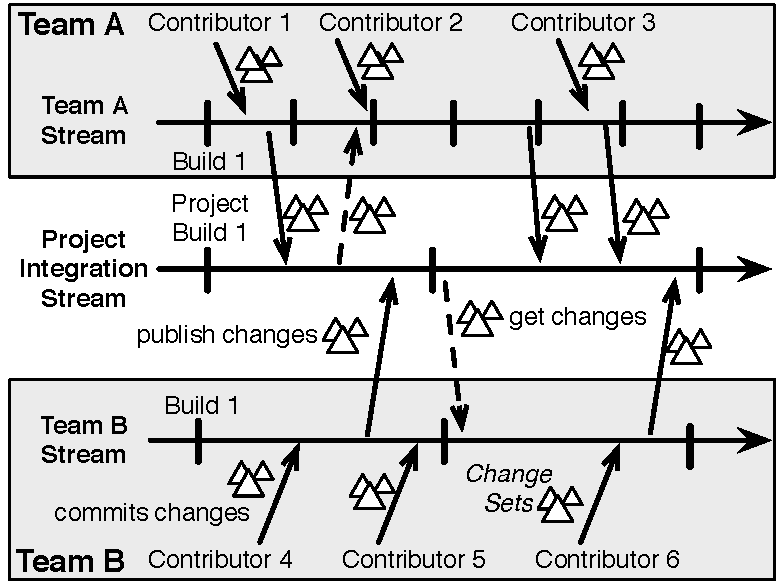
\includegraphics[width=8.3cm]{figures/BuildResult}
%\caption{Illustrates the exchange of change sets between different source code
%streams and the results of building the source code of the streams in time. Team
%members collaborate and interchange source code on a team related stream, while
%inter-team collaboration occurs on an integration stream.}
\caption{Teams contribute to their own source streams, which are then merged into one project stream.}
\label{fig:BuildResult}
\end{center}
\end{figure}


As illustrated in Figure~\ref{fig:BuildResult}, the coordination process within
each iteration requires the integration of subsystems developed by individual
Jazz teams in a major milestone build of the product (referred to as beta build).
Each team owns a source code \et{Stream} for collaboration and concurrent
implementation of the subsystem. A Stream is the Jazz equivalent to a branch of a
source configuration management system such as Subversion.

A continuous integration process takes place at team-level or project-level. In
frequent intervals, each integration build (referred to a build henceforth)
compiles, packages, and tests the source code of a stream. At the team-level,
contributors commit code changes that are encapsulated in \et{Change Sets} from
their own workspace to the \et{Team Stream}. The team integrations build the
subsystem developed by the team. Once a team has a stable version within the Team
Stream, the team publishes the change sets into the Jazz \et{Project Integration
Stream} (see Figure~\ref{fig:BuildResult}). At the project level, the automated
Jazz integration builds the subsystems of all teams. The Jazz project-level
integration takes place \et{nightly}, \et{weekly}, and at the end of each
iteration -- \et{beta} build.

\subsection{Coordination outcome measure}
In our study we conceptualize the coordination outcome by the \et{Build Result},
which is regarded as a coordination success indicator in Jazz and can be \error,
\texttt{WARNING} or \ok. We analyze build results to examine the integration
outcomes in relation to the communication necessary for the coordination of the
build.

Conceptually, the \texttt{WARNING} and \ok\ build results are treated similar by
the Jazz team, as they require no further attention or reaction from the
developers. In contrast, \error\ build results indicate serious problems such as
compile errors or test failures and require further coordination, communication
and development effort. We thus treated all \texttt{WARNING}s as \ok s to clearly
separate between failed and successful builds in our conceptualization of
coordination outcome.


\subsection{Communication in Jazz}

\et{Commenting} on work items is the main task-related communication and
collaboration channel used by Jazz. \et{Work Item}s represent single assignable
and traceable tasks. A set of work items defines the tasks for each team in each
iteration. Different types of work items represent defects, enhancements, and
general tasks. The work items are assigned to and owned by contributors. The
coordination necessary around the implementation of a work item is facilitated by
contributors commenting or observing the communication around work items.

\subsection{Communication measures}
To investigate the communication of contributors involved in an integration
build, we study the characteristics of the \emph{communication network} for each
build. In order to construct this network, we examine the content of the
\et{Change Set}s associated with the build. Whenever an integration is executed,
the change sets contain information on all changes made after the previous build,
and the work items associated with the changes. By identifying the contributors
who commented on these work items, we conceptualize communication among
contributors coordinating for the build by their commenting behavior.


\begin{figure}[t]
\begin{center}
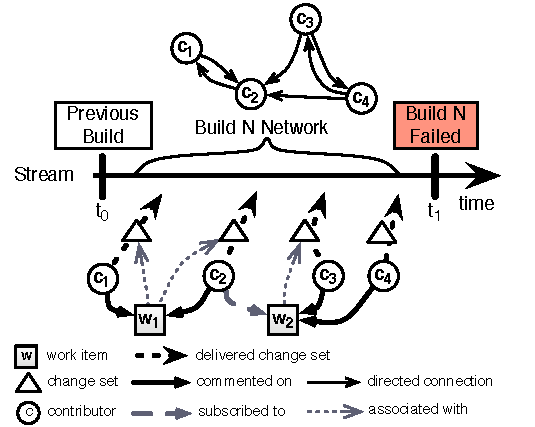
\includegraphics[width=7.5cm]{figures/BuildResultNetworks3}
%\caption{Illustrates the construction of communication networks in time, based on
%build results of a stream.}
\caption{Communication networks construction example for a failed Build N.}
\label{fig:NetworkConstructionExample}
\end{center}
\end{figure}

We use the example in Figure~\ref{fig:NetworkConstructionExample} to explain the
construction of communication networks. For a $Build~N$, the change sets made in
the time range $t_0$ to $t_1$ are used to construct the $Build~N~Network$, which
represents the communication that leads to $Build~N$. To construct the
\emph{communication network} for a build we consider that:

\begin{enumerate}
  \item the \emph{nodes} represent the contributors involved in the build or 
 its communication as follows:
  \begin{enumerate}
    \item committers of change sets involved in the build, as they have a
    direct impact on the build result
    \item creators, commenters, and subscribers on the work items associated with
    change sets, as they communicated on the build related tasks
  \end{enumerate}
  \item the \emph{directed connections} represent communication flow
  from contributor $c_i$ to $c_j$, communicating about a common set of
  work items that we name $WIs$ if:
  \begin{enumerate}
    \item $c_i$ is creator of or commenter on $WIs$ and provides
    information that is read by $c_j$
    \item $c_j$ is commenter or subscriber of any work items $WIs$ (assuming
    that $c_j$ reads all comments of $c_i$)
  \end{enumerate}
\end{enumerate}

For Build N in Figure~\ref{fig:NetworkConstructionExample} contributors $c_1$,
$c_2$, $c_3$, and $c_4$ delivered change sets to the stream in the time range $t_0$
to $t_1$. Thus, they are added to the associated Build N Network. To connect the
contributors in the network, we explore the work items $w_1$ and $w_2$ as they
are associated with the delivered change sets. The contributors $c_1$ and $c_2$
commented on $w_1$. As we assume that $c_2$ reads all comments of the work items
he comments on, we create a directed connection from $c_1$ to $c_2$, representing
the communication flow. Vice versa, we create a directed connection from $c_2$
and $c_1$. As $c_2$ is only subscribed to work item $w_2$ and did not add any
comments, we only create directed connections from $c_3$ and $c_4$ to $c_2$, as
those contributors commented on $w_2$. The resulting communication-based social
network Build N network represents the communication related to the development
that leads to the failed $Build~N$.

\subsection{Communication network measures}
To characterize the communication structure represented by the constructed
networks for each build, we compute a number of social network measures. The
measures that we include in our analysis are: Density, Centrality and Structural
holes. Some of these measures characterize single nodes and their neighbours (ego
networks), while others relate to complete networks. As we are interested in
analysing the characteristics of complete communication networks associated to
integration builds, we normalize and use appropriate formulas to measure the
complete communication networks instead of measuring the individual nodes.

% The following three subsections describe the formulas and give an example for
% each of the measures we included in our analysis.

\subsubsection{Density}
Density is calculated as the percentage of the existing connections to all
possible connections in the network. A fully connected network has a density of
1, while a network without any connections has the density of 0. For example, the
density in the directed network in Figure~\ref{fig:CentralityExample} is
$12/42=0.28$.

\subsubsection{Centrality measures}
We use the centrality measures \emph{group degree centralization} and
\emph{group betweenness centralization} for complete networks, which are based on
the ego network measures degree centrality and betweenness. The degree
centrality measures for the ego networks are:

\begin{itemize}
  \item The \emph{Out-Degree} of a node $c$ is the
  number of its outgoing connections $C_{oD}(c)$. E.g. $C_{oD}(c_1)=2$ in 
  Figure~\ref{fig:CentralityExample}.
% In our communication networks, the Out-Degree of a contributor $c$ in our is
% the number of other developers that read work items (AGAIN \ldots ``READ'' WORK
% ITEMS\ldots) and comments created by C.
  
  \item The \emph{In-Degree} of a node $c$ is the
  number of it s incoming connections $C_{iD}(c)$. E.g.$C_{iD}(c_1)=1$ 
  in Figure~\ref{fig:CentralityExample}.
% In our case, the In-Degree of a developer C in our communication network is the
% number of other developers from which the developer C read work items and
% comments.
  
  \item The \emph{InOut-Degree} of a node $c$ is the sum of its In-Degree and
  Out-Degree $C_{ioD}(c)$. E.g. $C_{ioD}(c_1)=3$
  in Figure~\ref{fig:CentralityExample}.
\end{itemize}

To compute the \emph{Group Degree Centralization} index for the complete network
we use formula~(\ref{eq:GroupDegreeCentralization}) from
Freeman~\cite{Freeman:1979rl}, in which $g$ is the number of nodes in a network,
and $C_D(c_i)$ is any of the degree centrality measures of a node $c_i$ as
described above. $C_D(c^*)$ is the largest node degree index for the set of
contributors in the network. The formula is also used
by~\cite{Gloor:2003cikm,hinds:cscw:2006}.

\begin{equation}
\displaystyle C_D =  \frac{\sum_{i=1}^g[C_D(c^*) - C_D(c_i)]}{(g-1)^2}
\label{eq:GroupDegreeCentralization}
\end{equation}

\begin{figure}[t]
\begin{center}
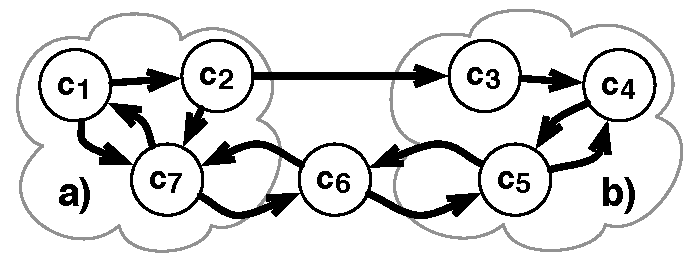
\includegraphics[width=5.0cm]{figures/CentralityExample}
\vspace{-10pt}
\caption{Example of a directed network to illustrate our social
analysis measures.}
\label{fig:CentralityExample}
\end{center}
\end{figure}

To calculate the \emph{Group Betweenness Centralization} index for a whole
network, we need to compute the betweenness centrality probability index for each
actor of the network. The probability index assumes that a ``communication''
takes the shortest path from a contributor $c_j$ to contributor $c_k$ and if the
network has more shortest paths, all of them have the same probability to be
chosen. If $g_{jk}$ is the number of shortest paths linking two contributors,
$1/g_{jk}$ is the probability of using one of the shortest paths for
communication. Let $g_{jk}(c_i)$ be the number of shortest paths linking two
contributors that contain the contributors $c_i$. Freeman~\cite{Freeman:1979rl}
estimates the probability that contributor $c_i$ is between $c_j$ and $c_k$ by
$g_{jk}(c_1)/g_{jk}$. The betweenness index for $c_i$ is the sum of all
probabilities over all pairs of actors excluding the $i$th contributor.
Formula~(\ref{eq:Betweenness}) shows the normalized betweenness index for
directed networks.

\begin{equation}
\displaystyle C_B(c_i) =  \frac{\sum_{j<k} g_{jk}(c_i)/g_{jk}}{(g-1)(g-2)}
\label{eq:Betweenness}
\end{equation}

To compute a betweenness index for the complete network instead of a single node,
we used Freeman's formula for \emph{Group Betweenness Centralization}. The
formula is shown in equation~(\ref{eq:GroupBetweenness}), in which $C_B(c^*)$ is
the largest betweenness index of all actors in the network.

\begin{equation}
\displaystyle C_B =  \frac{\sum_{i=1}^g[C_B(c^*)-C_B(c_i)]}{(g-1)}
\label{eq:GroupBetweenness}
\end{equation}


\subsubsection{Structural holes}
We use the following structural hole measures:
\begin{itemize}
  \item The \emph{Effective Size} of a node $c_i$ is the number of its
  neighbours minus the average degree of those in $c_i$'s ego network, not
  counting their connections to $c_i$. The effective size of node $c_1$ in 
  Figure~\ref{fig:CentralityExample}a is $2-1=1$. Note, that only direct
  neighbours of $c_1$ are considered and the directed connections are replace
  with undirected. The effective size of node $c_4$ in 
  Figure~\ref{fig:CentralityExample}b is $2-0=2$.
  
  \item The \emph{Efficiency} normalizes the effective size of a node $c_i$ by
  dividing the it's effective size with the number of it's neighbours. The
  efficiency of node $c_1$ in Figure~\ref{fig:CentralityExample}a is
  $(2-1)/2=0.5$. The efficiency of node $c_4$ in
  Figure~\ref{fig:CentralityExample}b is $(2-0)/2=1$.
  
  \item \emph{Constraint} is a summary measure that relates the connections of a
  node $c_i$ to the connections of $c_i$'s neighbours. If $c_i$'s neighbours and
  potential communication partners all have one another as potential communication
  partners, $c_i$ is highly constrained. If $c_i$'s neighbours do not have other
  alternatives in the neighborhood, they cannot constrain $c_i$'s behavior. 
\end{itemize}

To calculate network measures of the introduced ego network measures on
structural holes, we compute the sum of the measures for each node of a network.
As the measures are based on network connections, we normalize the sum by
computing the fraction of the sum and the number of possible network connections.

\subsection{Data collection} 

We mined the Jazz development repository for build and communication information.
A query plug-in was implemented to extract all development and communication
artifacts involved in each build from the Jazz server. These build-related
artifacts included build results, teams, change sets, work items, contributors,
and comments. We imported the resulting data into a relational database
management system to handle the data more efficiently.

We extracted a total of 1288 build results, 13020 change sets, 25713 work item
and 71019 comments. Out of a total of 47 Jazz teams, 24 had integration builds.
The build results we extracted were created during the time range from
November~5, 2007 to February~26, 2008.

Next, we had to make a decision for which builds and associated communication to
analyze. Our selection criteria was that we analyze a number of build results
that is large enough for statistical tests and include both \ok\ and \error\
builds. Some teams used the building process for testing puroses only and created
just a view build results, while others had either only \ok\ or only \error\
build results. Predicting build results for a team that only produced \error\
builds in the past, will most likely yield an \error, since no communication
information representing successful builds is available. Thus, we considered
teams that had more than 30 build results and at least 10 failed and 10
successful builds. Five teams satisfied these constraints and were considered in
our analysis. In addition, we included the nightly, weekly, and one beta
integration build, although they did not satisfy our constraints, because 
they integrate all subsystems of the entire project.






\section{Analysis and Results}
\label{sec:AnalysisResults}
% In this section we describe our analysis techniques for our research questions.
Table~\ref{tab:DescriptiveStats} shows descriptive statistics of the considered
builds and related communication networks of the five teams (B, C, F, P and W in
the first 5 columns) and the nightly, weekly, and beta project-level
integrations. For example, team B created 60 builds from which 20 turned out to
be \error s and 40 \ok. The communication networks of this team had between 3 and
58 contributors (51.58 directed connections in average) and spanned 0 to 131 work
items. The builds involved in average 10.83 change sets.

\begin{table}[t]
\footnotesize
\begin{center}
%{\small
\begin{tabular}{@{\hspace{1pt}}r@{\hspace{8pt}}c@{\hspace{5pt}}c@{\hspace{5pt}}c@{\hspace{5pt}}c@{\hspace{5pt}}c@{\hspace{5pt}}c@{\hspace{5pt}}c@{\hspace{5pt}}c@{\hspace{1pt}}}
\toprule
%  & & & Teams & & & & & &  \\
& \multicolumn{5}{ c@{\hspace{3pt}}}{Team Level Builds} &
\multicolumn{3}{c}{Project Level Builds} \\ & B & C & F & P & W & nightly &
weekly & beta
\\
\midrule
\# Builds & 60 & 48 & 55 & 59 & 55 & 15 & 15 & 16 \\ 
\# \error s & 20 & 16 & 24 & 29 & 31 & 9 & 11 & 13 \\ 
\# \ok s & 40 & 32 & 31 & 30 & 24 & 6 & 4 & 3 \\ 
%First Build & 2007-11-05 14:04:48 & 2007-11-09 07:22:05 & 2007-11-06 03:36:48
%& 2007-11-05 22:28:45 & 2007-11-09 17:01:35 & 2007-11-05 03:59:06 & 2007-07-24
%21:19:07 & 2007-12-04 14:23:20 \\ 
%Last Build & 2008-02-26 15:43:59 &
%2008-02-26 13:38:49 & 2008-02-22 16:34:25 & 2008-02-26 11:43:36 & 2008-02-26
%08:53:04 & 2008-01-18 07:41:26 & 2008-02-22 15:29:39 & 2008-01-23 19:22:41 \\
\midrule
\multicolumn{3}{l}{\emph{\# Contributors:}} \\
%\midrule
Min & 3 & 9 & 6 & 5 & 13 & 43 & 37 & 55 \\ 
Median & 6 & 16.5 & 18 & 15 & 20 & 55 & 57 & 69.5 \\ 
Mean & 12.68 & 18.02 & 20.15 & 17.98 & 22.87 & 57.93 & 52.27 & 67.81 \\ 
Max & 58 & 31 & 64 & 61 & 52 & 75 & 75 & 79 \\ 
\midrule
%\emph{Connections:}\\ 
\multicolumn{3}{l}{\emph{\# Directed Connections:}} \\
%\midrule
Min & 0 & 1 & 2 & 0 & 11 & 81 & 56 & 144 \\ 
Median & 13 & 39.5 & 95 & 36 & 74 & 236 & 149 & 280 \\ 
Mean & 51.58 & 53.4 & 87.78 & 63 & 88.35 & 253.1 & 171.9 & 285.8 \\ 
Max & 361 & 139 & 355 & 401 & 300 & 434 & 496 & 446 \\ 
\midrule
%\emph{Change Sets:}\\ 
\multicolumn{3}{l}{\emph{\# Change Sets:}} \\
%\midrule
Min & 1 & 15 & 8 & 32 & 83 & 80 & 62 & 82 \\ 
Median & 10 & 38 & 35 & 46 & 111 & 117 & 115 & 178.5 \\ 
Mean & 10.83 & 44.38 & 42.65 & 47.25 & 115.3 & 129 & 114.2 & 166.8 \\ 
Max & 33 & 101 & 91 & 75 & 156 & 199 & 173 & 196 \\ 
\midrule
%\emph{Work Items:}\\
\multicolumn{3}{l}{\emph{\# Work Items:}} \\
%\midrule 
Min & 0 & 2 & 1 & 1 & 10 & 11 & 5 & 31 \\ 
Median & 6.5 & 12 & 20 & 12 & 18 & 67 & 51 & 98 \\ 
Mean & 16.43 & 15.56 & 23.07 & 19.34 & 29.49 & 72.13 & 56.87 & 96.81 \\ 
Max & 131 & 50 & 100 & 107 & 119 & 132 & 202 & 170 \\ 
\bottomrule
\end{tabular}
\end{center}
\caption{Descriptive build statistics.}
\label{tab:DescriptiveStats}
\end{table}

\subsection{Individual communication measures and build results}
To examine whether any individual measure of communication structure can predict
integration failure or success (our Research Question 1), we analyze the builds
from each team and project-level integration in part in relation to the
communication structure measures as follows: For each team we categorize the
builds into two groups. One group contains the \error\ builds and the other the
\ok\ builds. For each build and associated communication network we compute the
network measures described in Section~\ref{sec:Methodology} and compare them
across the two groups of builds (\error\ and \ok).

The communication measures used in the analysis were: Density, Centrality
(in-degree, out-degree, inout-degree, and betweenness), Structural Holes
(efficiency, effective size, and constraint), and number of directed connections.
We used the Mann-Whitney test~\cite{Siegel:1956tu} to test if any of the measures
differentiate between the groups of \error\ and \ok\ related communication
networks. We used the $\alpha$-level of $.05$ and applied the Bonferroni
correction to mitigate the threat of multiple hypothesis testing. None of the
tests yielded statistical significance, which indicates that no individual
communication structure measures significantly differentiate between \error\ and
\ok\ builds.

We also tested for the possible effect of the technical measures shown in
Table~\ref{tab:DescriptiveStats}: \#Contributors, \#Change Sets and the \#Work
Items on the build result. Also, none of the tests yielded statistical
significance to differentiate between \error\ and \ok\ builds.


\subsection{Predictive power of combined measures of communication structures}

The second research question aims to assess whether the combination of
communication related network measures can predict future build results. Thus we
combined communication structure measures analyzed in RQ1 into a predictive model
that classifies a team's communication structure as leading to an \error\ or \ok\
build. We explicitly exclude the technical descriptive measures such as
\#Contributors, \#Change Sets and the \#Work Items from the model in order to
focus on the effect of communication on build failure prediction. We validate the
model for each set of team-level and project-level networks separately by
training a Bayesian classifier~\cite{Hastie:2003ys} and using the \emph{leave one
out cross validation} method~\cite{Hastie:2003ys}.

For example, to predict the build result N of team F's 55 build results, we train
a Bayesian classifier with all other 54 build results and their communication
related network measures. Then, we input the communication measures of Build N's
related communication network into the classifier and predict the result of build
N. We repeat the classification for all 55 builds of team F and sum up the number
of correctly and wrongly classified results.

\begin{table}[t] \centering\small
\begin{tabular}{lc}
& prediction \\
actual & 
\begin{tabular}{r|c|c|}
& \ok\ & \error\ \\\hline
\ok\ & 26 & 5 \\\hline
\error\ & 9 & 15 \\\hline
\end{tabular}
\end{tabular}
\caption{Classification results for team F.}
% \caption{Classification results for continuous build definition of team F, 26
% builds were correct as \ok\ and 5 wrong as \error\ classified.}
\label{tab:cont}
\end{table}

Table~\ref{tab:cont} shows the classification result for team F. The upper left
cell represents the number of correctly classified communication networks as
related to \ok\ builds (26 vs. 31 actual), and the lower right cell shows the
number of correctly classified networks as leading to \error\ builds (15 vs. 24
actual). The other two cells show the number of wrongly classified communication
networks.

The classification quality is assessed via recall and precision coefficients,
which can be calculated for \error\ and \ok\ build  predictions. We explain the
coefficients for prediction of \error\ builds.
% same definition as Tom's paper need to look up gail's definition

\begin{description}
\item[Recall] is the percentage of correctly classified networks as leading to
\error\ divided by the number of \error\ related networks. In
Table~\ref{tab:cont} the lower right cell shows the number of correct classified
networks that are leading to \error s, which is divided by the sum of the values
in the lower row, which represents the total number of actual \error s. This
yields for Table~\ref{tab:cont} a recall of $15/(9+15)=.62$. In other words,
62\% of the actual to \error\ leading networks are correctly classified.
 
\item[Precision] is the percentage of as to \error\ leading classified networks
that turned out to be actually \error s. In Table~\ref{tab:cont}, it is the
number of correctly classified \error s divided by the sum of the right column,
which represents the number of as \error\ classified builds. In
Table~\ref{tab:cont} the precision is $15/(5+15)=.75$. In practical terms, 75\%
of the \error\ predictions are actual \error s.
\end{description}




%\textbf{SVM} & & & & & & & & &  \\
%Error Recall & 55\% & 50\% & 62\% & 83\% & 48\% & 57\% & 56\% & 91\% & 92\% & 79\% \\
%Error Precision & 73\% & 73\% & 94\% & 80\% & 45\% & 66\% & 50\% & 71\% & 86\% & 67\% \\
%OK Recall & 89\% & 91\% & 97\% & 80\% & 25\% & 77\% & 17\% & 0\% & 33\% & 0\% \\
%OK Precision & 79\% & 78\% & 77\% & 83\% & 27\% & 70\% & 20\% & 0\% & 50\% & 0\% \\
%\hline

\begin{table}[t] \small
\begin{center}
%{\small
\begin{tabular}{ r@{\hspace{8pt}}c@{\hspace{5pt}}c@{\hspace{5pt}}c@{\hspace{5pt}}c@{\hspace{5pt}}c@{\hspace{5pt}}c@{\hspace{5pt}}c@{\hspace{5pt}}c}
\toprule
& \multicolumn{5}{ c@{\hspace{3pt}}}{Team Level Builds} &
\multicolumn{3}{c}{Project Level Builds} \\
%\textbf{Naive Bayes} & & & & & & & \\
& B & C & F & P & W & nightly & weekly & beta 	 \\
\midrule
\error\ Recall & .55 & .75 & .62 & .66 & .74 & .89 & 1 & .92 \\ 
\error\ Precision & .52 & .50 & .75 & .76 & .66 & .73 & .92 & .92 \\ 
\ok\ Recall & .75 & .62 & .84 & .80 & .50 & .50 & .75 & .67 \\ 
\ok\ Precision & .77 & .83 & .74 & .71 & .60 & .75 & 1 & .67 \\ 
\bottomrule
\end{tabular}
\end{center}
\caption{Recall and precision for \error\ and \ok\ build results using
the Bayesian classifier.}
\label{tab:PredictionResultTable}
\end{table}


We repeated the classification described above for each team and project-level
integration. Note that the model prediction results only show how the models
perform within a team and not across teams. Table~\ref{tab:PredictionResultTable}
shows the recall and precision values for as to \ok\ and \error\ leading
classified communication networks for each of the five team-level and three
project-level integrations. Since we are interested in the power of build failure
prediction, the error related values from our model are of greater importance to
us. The \error\ recall values (how many \error s were classified correctly) of
team-level builds are between 55\% and 75\% and the recall values of the
project-level builds are even higher with at least 89\%. The \error\ precision
values are equally high.





\section{Threats to validity}
We conceptualized \emph{communication} based on comments on work items. Besides
that, the Jazz team communicates via email, chat, web-based information and
face-to-face meetings. Based on our observations and conversations with the Jazz
team, we are certain that comments are mostly used to communicate about work
items. Since they are work item-specific and immediately available.

For the \emph{network construction}, we assumed that every developer commenting
on or subscribed to a work item reads all comments of that work item. This
assumption might not always be correct. By manual inspection of a selected number
of work items, we found that developers who commented on a work item are aware of
the other comments, confirming our assumption.

Due to storage problems the Jazz teams erased some build results. In the case of
nightly builds we expected 90 builds (according to project duration) but found
only 15. This might affect our results but we argue that due to our richness of
data the general trend is still preserved. Hence we expect that our findings
would be supported by the complete data, too.

Our results are only valid for the Jazz project and can not be generalized to
any software development project. Additional studies on different projects
using Jazz could be conducted to confirm our results.



\section{Discussion}
\label{sec:discussion}
As far as we know, our study is one of the first to investigate communication
structures at the level of integration builds. This is a finer-grain level of
analysis than that of current studies in the literature, which found that
coordination failures are due to communication problems. By conceptualizing
coordination failure as a failed integration result, we studied the role of
communication structures in successful coordination. In
Section~\ref{subsec:commaspred} we discuss our contribution which is two-fold:
(1) while communication structure measures can not individually predict failed
builds, (2) a set of communication structure measures can be combined into a
model that predicts failed integration builds. Subsequently, we discuss practical
implications of our work in Subsection~\ref{subsec:practicalimpl}.

\subsection{Communication as predictor for integration failure}
\label{subsec:commaspred}
In our analysis we examined the relationship between integration builds and
measures of the related communication structure. We found that none of the single
communication structure measures (density, centrality or structure hole measures)
significantly differentiated between failed and successful builds at the
team-level and project-level. Therefore none of these individual communication
structure measures could be used to predict integration build results.


In addition to the communication related measures, we also examined whether the
technical measures we computed when constructing the communication networks --
the number of change sets, contributors, and work items -- have an impact on the
integration build result, as they are an indication for the size and complexity
of the development tasks to be coordinated. According to Nagappan and
Ball~\cite{nagappan2005:churn}, one might expect that increased size and complexity
of code changes relates to more build failures. But in our study these single
measures did not significantly differentiate between successful and failed build
results. However, additional technical measures that were used by Nagappan might
be good predictors in Jazz as well.

%Thus, the communication structures seem to be more important and
%can cope with task complexity and size.


The second contribution of this work is the predictive model that uses measures
of communication structures to predict build results. Interestingly, the
combination of communication structure measures was a good predictor of failure
even when the single measurements were not. Our model's precision in predicting
failed builds, which relates to the confidence one can have in the predicted
result, ranges from 50\% to 76\% for any of the five team-level integration
builds, and is above 73\% for the project-level integration builds.

We found that, for all prediction models, the recall and precision values are
better than guessing. A guess is deciding on the probability of an \error\ or an
\ok\ build if the build fails or succeeds. The probability is the number of
\error s or \ok s divided by the number of all builds. For example, if we know
that the \error\ probability is 50\% and we guess the result of the next build we
would achieve a recall and precision of 50\%. In our case, our model reached an
\error\ recall of 62\% for team F, where as a guess would have yield only
$24/55=.44=$ 44\% (see Table~\ref{tab:DescriptiveStats}).

\subsection{Practical implications}
\label{subsec:practicalimpl}

\begin{figure}[t]
\begin{center}
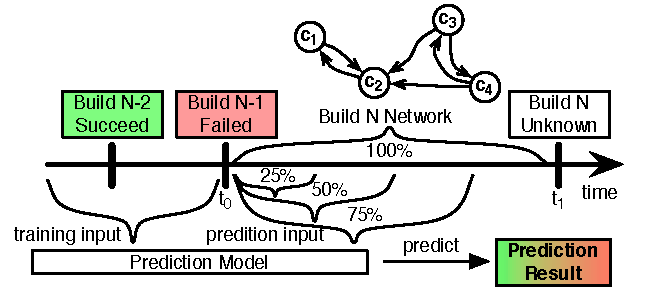
\includegraphics[width=8.4cm]{figures/ReducedCommunicationInput}
\caption{Predicting Build N Result with different reduced communication
data.}
\label{fig:ReducedCommunicationInput}
\end{center}
\end{figure}



%\textbf{SVM} & & & & & & & & &  \\
%Error Recall & 55\% & 50\% & 62\% & 83\% & 48\% & 57\% & 56\% & 91\% & 92\% & 79\% \\
%Error Precision & 73\% & 73\% & 94\% & 80\% & 45\% & 66\% & 50\% & 71\% & 86\% & 67\% \\
%OK Recall & 89\% & 91\% & 97\% & 80\% & 25\% & 77\% & 17\% & 0\% & 33\% & 0\% \\
%OK Precision & 79\% & 78\% & 77\% & 83\% & 27\% & 70\% & 20\% & 0\% & 50\% & 0\% \\
%\hline

\begin{table}[b]
\small
\begin{center}
%{\small
\begin{tabular}{ r@{\hspace{8pt}}c@{\hspace{5pt}}c@{\hspace{5pt}}c@{\hspace{5pt}}c@{\hspace{5pt}}c@{\hspace{5pt}}c@{\hspace{5pt}}c@{\hspace{5pt}}c}
\toprule
& \multicolumn{5}{ c@{\hspace{3pt}}}{Team Level Builds} &
\multicolumn{3}{c}{Project Level Builds} \\
%\textbf{Naive Bayes} & & & & & & & \\
& B & C & F & P & W & nightly & weekly & beta 	 \\
\midrule
\error\ Recall & .63 & .69 & .62 & .62 & .68 & 1 & .45 & .85 \\ 
\error\ Precision & .43 & .46 & .68 & .75 & .64 & .75 & .83 & .92 \\ 
\ok\ Recall & .60 & .59 & .77 & .80 & .50 & .50 & .75 & .67 \\ 
\ok\ Precision & .77 & .79 & .73 & .69 & .55 & 1 & .33 & .50 \\  
\bottomrule
\end{tabular}
\end{center}
\caption{Recall and precision results only including first 25\% of the
communication.}
\label{tab:Prediction25PResultTable}
\end{table}


Our model can be used by Jazz teams to assess the quality of their current
communication in relation to the result of their upcoming integration. If a team
is currently working on a component and an integration build is planned in the
near future, the measures of the current communication in the team can be
provided as input to our prediction model and the model will predict whether the
build will fail with a precision shown in Table~\ref{tab:PredictionResultTable}.
For example, if team P is working towards a build and our model predicts that the
structure of its current communication leads to a failed build, the team can have
a 76\% (see Table~\ref{tab:PredictionResultTable}) confidence that the build is
going to fail. This information can be used by developers in monitoring their
team communication behavior, or by management in decisions with respect to
adjusting collaborative tools or processes towards improving the integration.

In our analysis we used the complete communication of the build related time
interval as input for the model to predict the build result. In
Figure~\ref{fig:ReducedCommunicationInput}, this is the time interval from $t_0$
to $t_1$ for $Build~N$. This time interval might not be appropriate for practical
applications in which the build process takes only a view minutes, as $t_1$ is
immediately before the build starts. Predicting the build result has no value for
the developers when they have no time left to react on a build failure prediction
and they can simply run the build instead of predicting the result. For long
builds that last several days, the prediction at $t_1$ is still practical
relevant. Developers might delay the build to perform reactive changes on the
failure prediction.

In an additional analysis we investigated the prediction recall and precision by
only considering the communication of reduced time intervals as input for our
model. For each build N result, we trained our model with the complete
communication of all build results except the one from N, and predicted the
result N by only considering the first 25\%, 50\% and 75\% of the communication
as input for the prediction model (see
Figure~\ref{fig:ReducedCommunicationInput}).

We only show the precision and recall of the prediction for the 25\% time range
in Table~\ref{tab:Prediction25PResultTable}, as they are already high enough for
practical use. We observe that the model has almost the same predictive power as
the model considering the complete time range of the build. A possible
explanation is the involvement of work items in many builds. That means that the
task completion time of a work item is longer than the time interval of a build
and task related change sets and communication occurs in multiple builds. When a
developer delivers a change set in the first 25\% of the build related time
interval and the change set is associated to a work item that has already been
discussed, the complete past communication is included. Including the past
communication is valid, as our prediction model learns from the communication
history. In Jazz, a work item is in average included in 5.17 builds (min=1,
median=3, max=57), which provides a possible explanation for having valuable
prediction results even early in the build related time interval.

With the results of this analysis, we are confident that our prediction model is
practically useful, even if it does not consider the complete communication of a
build. Thus, developers and managers have time to react on build failure
predictions before the actual build fails.




\section{Conclusion}
\label{sec:conclusion}
Our results indicate that developer communication plays an important role in the
quality of software integrations. Complementary to existing literature on
communication and coordination outcome in software engineering, we objectively
measured coordination outcome by the result of the integration build. To capture
and study communication we used social network measures. Although we found that
no individual social network measure could indicate whether a build will fail or
succeed, the combination of network measures can be combined into a predictive
model. The model indicates whether an integration will fail based on the current
communication structure of a development team. For five project studied teams,
our predictive model yielded recall values between 55\% and 75\%, and precision
values between 50\% to 76\%.

The study of communication patterns in relation to team performance is important
given that communication is the main mechanism for knowledge sharing in work
groups. Software engineers differ in the expertise, knowledge, and background
they bring to the development task. Group performance depends not only on the
information available to developers and the knowledge distribution within the
team, but also on the properties of the communication structure that facilitates
knowledge dissemination.

Having identified that communication plays an important role in
integration success, future research should examine the interaction with other factors
that could determine integration failure. In addition to our focus of
communication, the analysis of code and code changes should be considered. We
believe that a combination of both will lead to even better prediction models for
software integration builds.

Based on the information provided by our predictive model, awareness systems can
be developed to provide recommendations to improving a team's communication
structure when developers face a likly build failure. We intend to integrate our
predictive model into the Jazz development environment itself, and provide
developers and managers with a real-time communication quality feedback mechanism
that would predict possible failed builds based on the current communication
behavior in the project. This will give us the opportunity to evaluate the value
of our predictions with respect to improvements in software coordination.


%%%%%%%%%%%%%%%%%%%%%%%%%%%%%%%%%%%%%%%%%%%%%%%%%%%
%%%%%%%%%%%%%%%%%%%%%%%%%%%%%%%%%%%%%%%%%%%%%%%%%%%
%%%%%%%%%%%%%%%%%%%%%%%%%%%%%%%%%%%%%%%%%%%%%%%%%%%
%%%%%%%%%%%%%%%%%%%%%%%%%%%%%%%%%%%%%%%%%%%%%%%%%%%
%%%%%%%%%%%%%%%%%%%%%%%%%%%%%%%%%%%%%%%%%%%%%%%%%%%

\startchapter{Socio-Technical Congruence and Failure}
We hypothesize that with the ever growing size of software teams the lack of
effective coordination is the main source of integration failures.  With the
ever growing complexity and sophistication of large software projects,
error-free integrations are not only important but difficult to achieve. The
development work that precedes integrations involves significant coordination of
developers that work in teams and need to rely on the code of others and its
stability. But often code is everything but stable, further contributing to
developers' need to coordinate to keep up with code changes that impact their work. This problem is
amplified in software builds where an entire team needs to integrate their work
and on which the development of new features depends. Not only do
failed builds destabilize the product~\cite{cusumano1997} but they also demotivate
software developers~\cite{holck2004}.

Despite their importance, keeping integrations builds error-free can be a very time consuming
process. A lightweight approach that can determine whether the build contains
failures before invoking the build process is thus very valuable to developers.
This lightweight approach could determine a builds outcome in minutes rather than hours or days. Having a faster way to
assess the quality of a build helps developers to continue working with newest
builds while being aware of its quality. Previous
research~\cite{wolf:icse:2009,hassan:ase:2006} trained predictive models to assess the quality of software builds without the need of invoking large test
suits. Although this research
reaches a high degree of accuracy in their predictions, knowing that a
build will fail does not necessarily help developers to actually prevent
the build from failing.
% limitation of previous research
% SENTENCE HERE ABOUT WHY THIS IS A PROBLEM. SENTENCE ABOUT HOW THIS WAS STUDIED
% BEFORE AND THE LIMITATION THAT RESEARCH HAD ONLY STUDIED PRECTIVE MODELS
% WITHOUT THE ABILITY TO ACT ON THAT KNOWLEDGE.
The goal of this research is to find a way to create actionable knowledge that
developers can act upon to avoid
integration failure.

In this paper we describe a case study of IBM's Jazz project where we leverage
information about socio-technical developer coordination and software builds to
identify pairs of developers that negatively influence the quality of the
upcoming build. Using historical project information we construct socio-technical
networks that capture information about developers with technical dependencies
as well as their ongoing communication as conceptualization of their coordination.
We found that using a support vector machine on a combination of this social
and technical project data yields a powerful predictor of build failure. We
then identify that there are certain pairs of developers that have a
negative influence on the build outcome. On this knowledge developers and management can
act upon to avoid future build failure.

Maintaining proper communication and awareness of work others perform is
important in any kind of project. Specifically in software engineering many studies found
that factors such as geographical and organizational distance have an impact on
communication and even effect software quality~\cite{nagappan:icse:2008}. In our
study we uncover the existence of pairs of
developers, that, if technically dependent in a build but not discussing their
dependencies, have a negative influence on the success on builds. This
actionable knowledge can be integrated in real-time recommender systems that
indicate, based on project historical data, which developer pairs tend to be
failure related. Developers and management can then devise strategies to
prevent the failure before build time. 


The paper is organized as follows: We start with formulating our research
questions (Section~\ref{sec:rq}) followed by putting our research into the
perspective of related work (Section~\ref{sec:relwork}). Section~\ref{sec:data}
covers details about our case study of IBM's Jazz team to investigate
socio-technical coordination in relation to builds. Then
Sections~\ref{sec:prediction} and \ref{sec:pattern} cover the actual analysis and
their discussion. Before we concluding the paper in
Section~\ref{sec:conclusions}, we discuss some practical implications in Section~\ref{sec:implications} and the threats to validity
(Section~\ref{sec:threats}).



%  ONCE SENTENCE HERE REMINDING THE READER THAT IN THIS PAPER WE PROPOSE A
% LIGHTWEIGHT APPROACH THAT LEVERAGES DEVELOPERS SOCIAL NETWORKS BUILT FROM
% PROJECT HISTORICAL DATA AND WHICH IDENTIFIES WHICH DEVELOPER PAIRS ARE
% IMPORTANT WITH RESPECT TO THE QUALITY OF THE UPCOMING BUILD.

\section{Research Questions}
\label{sec:rq}
Communication
is an important mechanism for coordination in software development \cite{curtis:acm:1988,kraut:1995coordination}, especially in maintaining the awareness of changes relevant to your work. Past research showed that a high coverage of technical
dependencies by social relationships correlates with higher productivity of development teams (e.g.~\cite{cataldo:cscw:2006}). 
 We hypothesize that a similar relation
exists between this coverage and the success of software builds. 

Thus
socio-technical networks that capture information about the social and technical
relationships between developers, should predict build failure:

\begin{itemize}
\item[RQ1] Can we use information about relations (technical and social) between
developers to predict build outcome?
\end{itemize}

Although valuable, having a model that predicts build outcome is often not
enough. We seek to generate actionable knowledge upon which developer can act to
avoid a build from failing. Past research suggests that the absence of
communication between developers that are technically dependent leads to
problems, such as slow down in development~\cite{cataldo:esem:2008}.


We hypothesize that due to the high coordination needs the absence of this
important communication also has a negative influence on build outcome. Communication problems can arise from many factors including organizational,
social or technical reasons. Being able to pinpoint
mismatches between technical dependencies and required communication that
relate to build failure is even more important in a team's
ability to devise strategies to avoid build failure. Thus, we
investigate pairs of developers that share a technical dependency without talking
with each other (referred to as \emph{technical pairs}):


\begin{itemize}
\item[RQ2] Are there technical pairs that influence the build outcome?
\end{itemize}

Acknowledging that build failure can be the result
of factors other than lack of developer
communication, e.g. the number of changes or developers in a build~\cite{hassan:ase:2006}, our
analysis also studies the effect of technical pairs in the presence of such
confounding variables. 





%The answer to this question will tell us if we really can devise strategies to
%prevent builds from failing. 


\section{Related Work}
\label{sec:relwork}
Our study aims on integrating work investigating team collaboration and failure prediction to produce actionable knowledge upon which developer can act.
Several studies bear relevance with respect to different dimensions of our work:

\emph{With respect to research on software builds:}
To the best of our knowledge the studies by Hassan et al.~\cite{hassan:ase:2006}
and Wolf et al.~\cite{wolf:icse:2009} are the only studies that conducted
research to predict build outcome. Hassan et al.~\cite{hassan:ase:2006} found
that a combination of social metrics (e.g. number of authors) and technical
metrics (e.g. number of code changes) derived from the source code repository
yield to be best predictor. On the other hand Wolf et al.~\cite{wolf:icse:2009}
solely used metrics that they derived from the social network created from
discussions among developers and showed that communication structure has an
influence on the build outcome.

\emph{With respect to team coordination:}
%Coordination is defined as ``integrating or linking together different parts of
%an organization to accomplish a collective set of tasks''~\cite{vandeven1976}. 
In
order to manage changes and maintain quality, developers must coordinate. In
software development, coordination is largely achieved through communicating with
people who depend on the work that you do \cite{kraut:1995coordination}. The
software engineering literature is recognizing the role of communication as
something that should be nurtured not eliminated and recent
collaborative software development environments aim to support developers'
social interactions along with artifact creation activities~\cite{nakakoji2010:rdc}.

%While a failed build is not necessarily a disaster, it slows down work significantly and is considered extremely undesirable.
%A build result thus serves as an indicator of the health of the software project up until that point in time. If the developers successfully coordinate the integration of code between the previous build and the upcoming build, then the build should succeed.

Ehrlich et al.~\cite{ehrlich:icgse:2006} investgiated how social networks can be
used to leverage knowledge in distributed teams. Backstrom et
al.~\cite{backstrom:kdd:2006} took a more general approach and investigated the
evolution of large social networks and the information they hold. Chung et
al.~\cite{chung:cpr:07} reported in recent work about behavior of individuals
while performing knowledge intensive tasks. There have been a number of studies
that investigated communication structures to identify good
coordination practices
(e.g.~\cite{hinds:cscw:2006,hossain:cscw:2006,bird:fse:2008,hinds:hicss:2008}). In contrast to studies of the general development process, Marczak studied social
networks to identify best practices for requirements management
processes~\cite{marczak:re:2008}.

Inspired by Conways Law~\cite{conway:datamination:1968}, Cataldo et
al.~\cite{cataldo:cscw:2006,cataldo:esem:2008} formulated a coefficient that
measures the alignment of the social and technical networks defining the term of
socio-technical congruence. They observed that higher socio-technical congruence
leads to higher developer
productivity~\cite{cataldo:cscw:2006,cataldo:esem:2008}. Others used this
notion and coefficient to further investigate the effect of congruence
(e.g.~\cite{valetto:msr:2007}). Prior to Cataldo et
al.~\cite{cataldo:cscw:2006,cataldo:esem:2008} proposal,
Ducheneaut~\cite{ducheneaut:cscw:2005} investigated the evolution of social and
technical relationships of open source project participants to see how those
participants become a part of the community.


\emph{With respect to failure prediction:}
There have been a large number of studies looking into predicting failures. For
example, Zimmermann et al.~\cite{zimmermann:icse:2008} used
networks constructed from interdependent binaries to predict the failure
probability of files. They used different metrics characterizing the relationship
binaries have to each other and found that ego centric social network measures
are powerful failure predictors. Previous research conducted at Microsoft used
code complexity metrics, such as cyclomatic complexity or object oriented
metrics, that are derived from source code. Nagappan et
al.~\cite{nagappan:icse:2006} found
that no single source code metric was capable of being a good
predictor over all studied Microsoft projects. Motivated by this study that
suggested that predictions might be domain specific Schr\"oter et
al.~\cite{schroeter:isese:2006} characterized domain of packages in the Eclipse
project by their imports and found them to be a powerful predictor.


\emph{With respect to failures related to team coordination:}
More recent studies started to relate the social with the technical
dimensions of software development to build predictive models. Pinzger et
al.~\cite{pinzger:fse:2008} successfully used social networks connecting
developers via code artifacts to predict failures. Meneely et
al.~\cite{meneely:fse:2008} used similar networks but excluded the code artifacts
and connected the developers directly. Two studies at Microsoft looked into the
geographical~\cite{bird:acm:2009} and organizational~\cite{nagappan:icse:2008}
distance between people that worked on the same binary and the relation to the
failure proneness of said binary. They found that the organizational distance is
a very powerful predictor of failure proneness of binaries whereas the
investigation of geographical distance has little to no effect. A recent
study~\cite{bird:issre:2009} combines the work of Pinzger et
al.~\cite{pinzger:fse:2008} and
Zimmermann~\cite{zimmermann:icse:2008} by creating
socio-technical networks that capture developer contributions and binary
interdependencies. They found this combination to be a more powerful predictor
that works for different software project and even prevails across multiple
revisions of a project.

% talk about the short coming of the failure prediction models
Despite the high predictive power of the state-of-the-art prediction models, most
of them suffer from a profound shortcoming: the knowledge provided by these
models is not always easily actionable. In this work we lie the foundation to
the recommender system described by Schr\"oter et
al.~\cite{schroeter:rsse:2008}. 
%
This recommender system compares social networks derived from technical and social dependencies over successful and failed builds to recommend changing failure related pairs of developers.
%
%AND WHICH\ldots A BIT MORE HERE ABOUT HOW THIS
%RECOMMENDER SYSTEM MAY WORK BASED ON THE RESULTS OF THIS WORK (YOU CAN REPLACE
%THE NEXT SENTENCE WITH THIS DETAIL IF SPACE IS A PROBLEM). 
%
This way we generate knowledge that not only tells us when a build fails but immediately helps us to provide suggestions to prevent the build from failing.





%\pagebreak



\begin{table}[t]
\centering
\begin{tabular}{rrccc}
\toprule
& & Successful & Failed & Total\\
\midrule
&min &1&1&1\\
\#work item & avg  & 16.68&26.52&19.63\\
& max & 111&109&111\\
\midrule
& min & 1&1&1\\
\#change set & avg  & 26.71&46.27&32.57\\
& max & 227&194&227\\
\midrule
& min & 1&1&1\\
\#Developers & avg  & 19.62&28&22.16\\
& max &64&71&71\\
\bottomrule
\end{tabular}
\caption{Statistics on Jazz data: change sets, work items, 
and developers over successful (227), failed (99) and total builds (328).}
\label{tab:jazzbuildinfo}
\end{table}

\begin{figure}[b]
\centering
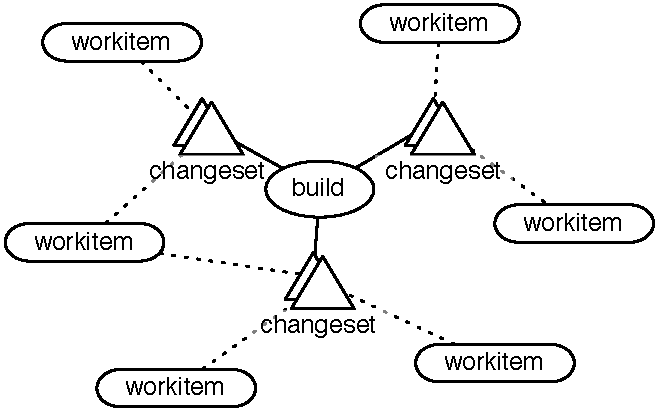
\includegraphics[width=.9\columnwidth]{figures/buildworkitem}
%\vspace{-.3cm}
\caption{Linking work items to builds using change sets.}
\label{fig:buildtowork item}
\end{figure}

\begin{figure}[t]
\centering
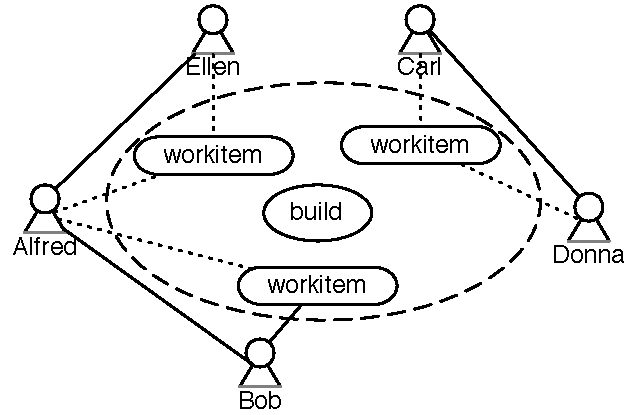
\includegraphics[width=.9\columnwidth]{figures/buildsn}
%\vspace{-.3cm}
\caption{Social network connecting developers through discussions about
work items in a build}
\label{fig:buildsn}
\end{figure}


















\section{Socio-technical coordination\\ and builds in Jazz}
\label{sec:data}
Before we describe our approach to collect data and construct
socio-technical networks in Jazz, we give a brief
description of the Jazz\texttrademark\ team and project. Subsequent,
we explain our approach of mining the project archives to construct
socio-technical networks (Subsections~\ref{subsec:social}
and~\ref{subsec:technical}).

\subsection{Development and Builds in the Jazz Team}
%\subsection{Coordination and integration in Jazz}
The Jazz\tm\ team is a large distributed team and uses the Jazz\tm\ platform for
development. The Jazz\tm\ development involves distributed collaboration over 16
different sites located in the United States, Canada, and Europe. Seven sites are
active in Jazz development and testing. There are 151 active contributors
working in 47 teams at these locations, where developers can belong to multiple
teams. Each team is responsible for developing a subsystem or component of Jazz\tm\.
The team size ranges from 1 to 20 and has an average of 5.7 members. The number
of developers per geographical site ranges from 7 to 24 and is 14.8 in average.

The project uses the \emph{Eclipse Way} development process~\cite{frost:ieeesoftware:2007}.
It defines six-week iteration cycles, which are separated into planning,
development and stabilization activities. A project management committee
formulates the goals and features for each release at the beginning of the each
iteration, and \emph{work items} represent assignable and traceable tasks for each
team.
Furthermore, the Jazz\texttrademark\ team's development process demands that the developers coordinate using work item discussion. 

The coordination process within
each iteration requires the integration of subsystems developed by individual
Jazz\tm\ teams in a major milestone build of the product.
Each team owns a source code Stream for collaboration and concurrent
implementation of the subsystem. A Stream is the Jazz\tm\ equivalent to a branch of a
source configuration management system, such as Subversion.

A continuous integration process takes place at team-level or project-level. In
frequent intervals, each integration build (referred to a build henceforth)
compiles, packages, and tests the source code of a stream. At the team-level,
contributors commit code changes that are encapsulated in change sets from
their own workspace to the Team Stream. The team integrations build the
subsystem developed by the team. Once a team has a stable version within the Team
Stream, the team publishes the change sets into the Jazz\tm\ Project Integration
Stream. At the project level, the automated
Jazz\tm\ integration builds the subsystems of all teams. 
%The Jazz project-level
%integration takes place \et{nightly}, \et{weekly}, and at the end of each
%iteration -- \et{beta} build.

%%%%%%%%%%%


%We analyze builds created by IBM's Jazz\texttrademark\ development team.
%The Jazz team builds on a regular basis on a nightly and weekly basis.
%Those builds are both on a component and on a project basis.
%
%The Jazz team uses the software they develop the IBM Jazz\texttrademark.
%IBM Jazz\tm\ integrates both source code control and task management.
%Additionally you can also define build schedules as well as general development processes, such as SCRUM.
%
%Thus, the Jazz repository contains all the information from builds over source code changes to tasks, such as bug fixes.
%One advantage of working with he Jazz repository is that links between builds and changes, and changes and tasks are explicit.
%This means we know from the repository which changes contributed to a build and which changes where made to accomplish a task.
%Using this information we can infer which tasks influenced which builds.
%
%The Jazz development team follows the Eclipse Way of development~\cite{frost:ieeesoftware:2007}.
%The team was between April and July 2008 on a six week development cycle during which a set of features and bug fixes needs to be implemented.
%Instead of extending the cycles when features or bug fixes would take longer to complete they reschedule it for the next cycle.
%
%Another important aspect to their process directly impacts the way they communicate or record their communication.
%Since the Jazz development team is distributed across several sites in North America and Europe they implemented a process that enforces them to record all their communication around any task in the repository.
%This is a best practice implemented by the former Eclipse developer to ensure that people offside do know what's going on and to enable them to contribute.

% some stats about the repository and the team
We mined the Jazz project repository between April and July 2008, and analyzed a
total of 328 builds, out of which 99 were failed and 227 were successful.
Table~\ref{tab:jazzbuildinfo} contains summary statistics describing the Jazz\tm\
repository. We report different aggregations (minimum, average and maximum) of
number of work items, change sets, and developers over all builds. 


%%%%%%%%%%%%%%%%%%%%%%%%%%%%%%%%%%%%%%%%%%%%%%%%%%%%%

%\begin{figure}[t]
%\centering
%\includegraphics[width=.9\columnwidth]{cochangedfiles}
%%\vspace{-.3cm}
%\caption{Conceptualization of technical relation using co-changed files.}
%\label{fig:technicaldependency}
%\end{figure}

\begin{figure*}[t]
\centering
\subfloat[Identify all change sets related to the social network's build.]{
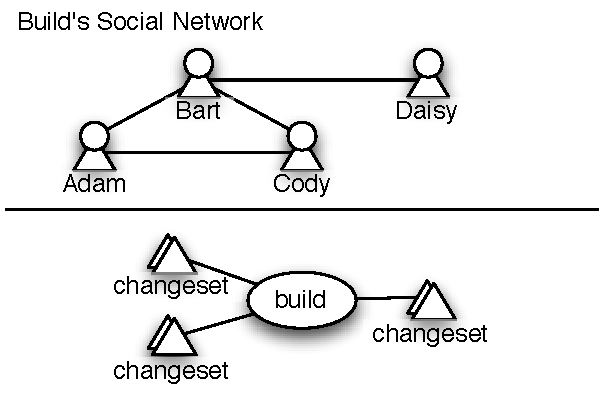
\includegraphics[width=.65\columnwidth]{figures/idcs}
\label{subfig:idcs}
}
\quad
\subfloat[Adding change set owners that are not part of the social network.]{
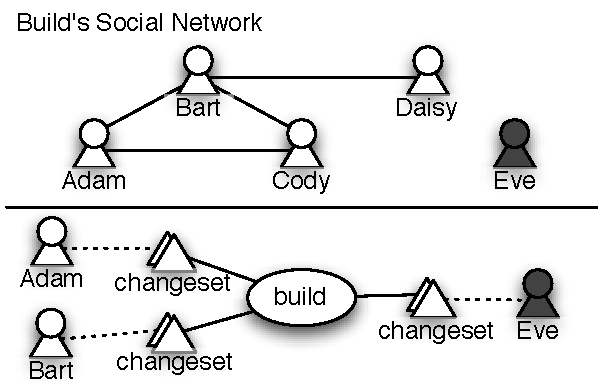
\includegraphics[width=.65\columnwidth]{figures/adduser}
\label{subfig:adduser}
}
\quad
\subfloat[Connect Adam and Bart with a technical edge via the co-changed File$_A$.]{
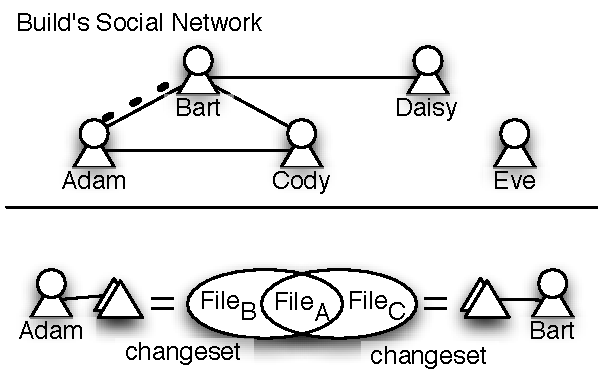
\includegraphics[width=.65\columnwidth]{figures/addedge}
\label{subfig:addedge}
}
%\vspace{-.2cm}
\caption{
Creating a socio-technical network by adding technical dependencies to a build's social-network.}
\label{fig:addtechnicaledge}
\end{figure*}





\subsection{Extracting Social Networks}
\label{subsec:social}
To model the communication between developers for a given build we construct \emph{social networks}. 
We use the information contained in the Jazz\texttrademark\ work items for the construction. 
A \emph{work item} in Jazz\texttrademark\ is the basic unit of work. 
It describes a general task which can be, but is not restricted to, a bug fix or feature request.
Developers coordinate about work on work items by posting comments in a discussion board style which we use as conceptualization of their coordination behavior.
Note that the communication through board discussions is enforced by the team's development process. 


We are interested in constructing a social network for each
build in Jazz\texttrademark. 
To create a social network for a given build we proceed in six steps:

\begin{enumerate}
\item Select the build of interest.
\item Extract change sets that are part of the build.
\item Extract work items linked to the retrieved change sets.
\item Extract developers commenting on a work item before the build's built time.
%\item Retrieve developers that created the retrieved work items.
\item Connect all developers commenting on the same work item.
\end{enumerate}

These steps take us as illustrated in Figure~\ref{fig:buildtowork item}
from a build through a change set to a work item. From the work item we are able to
see who contributed to the work item discussion (Figure~\ref{fig:buildsn}).
These developers become part of the social network and
share a \emph{social edge} if they made a comment on the same work item.
% We use the term \emph{social edge} to describe this connection between two
% developer that commented on the same work item.
Note that all links we use to get from a build to a developer are explicitly contained in
the Jazz\texttrademark\ repository.




\subsection{Constructing Socio-Technical Networks}
\label{subsec:technical}
%\todo{why only change dependencies}
Past research~\cite{nagappan:icse:2005} has shown that dynamic dependencies have the strongest influence on the software quality.
Therefore we use these dynamic dependencies
to construct \emph{socio-technical networks} we use the steps described below
(see Figure~\ref{fig:addtechnicaledge}). We essentially add technical edges to
the build's already constructed social network. In our conceptualization a \emph{technical edge} is a source code
dependency between two developers. A technical dependency between two developers
exists if they changed the same source code file in the build of interest. 

\begin{enumerate}
\item Extract the change sets that are part the build (Figure~\ref{subfig:idcs}).
\item Determine change set owners and add those  that are not already part
of the social network (Figure~\ref{subfig:adduser}).
\item Add a technical edge between change set owners that did change the same file (see Figure~\ref{subfig:addedge}).
\end{enumerate}


We thus call a network that contains both social and technical edges a
\emph{socio-technical network}. The developers in the 
socio-technical network that share both a technical and social edge are said to share
a \emph{socio-technical edge}.











\begin{figure*}[t]
\centering
\subfloat[Evaluation results from the Support Vector Machine.] {
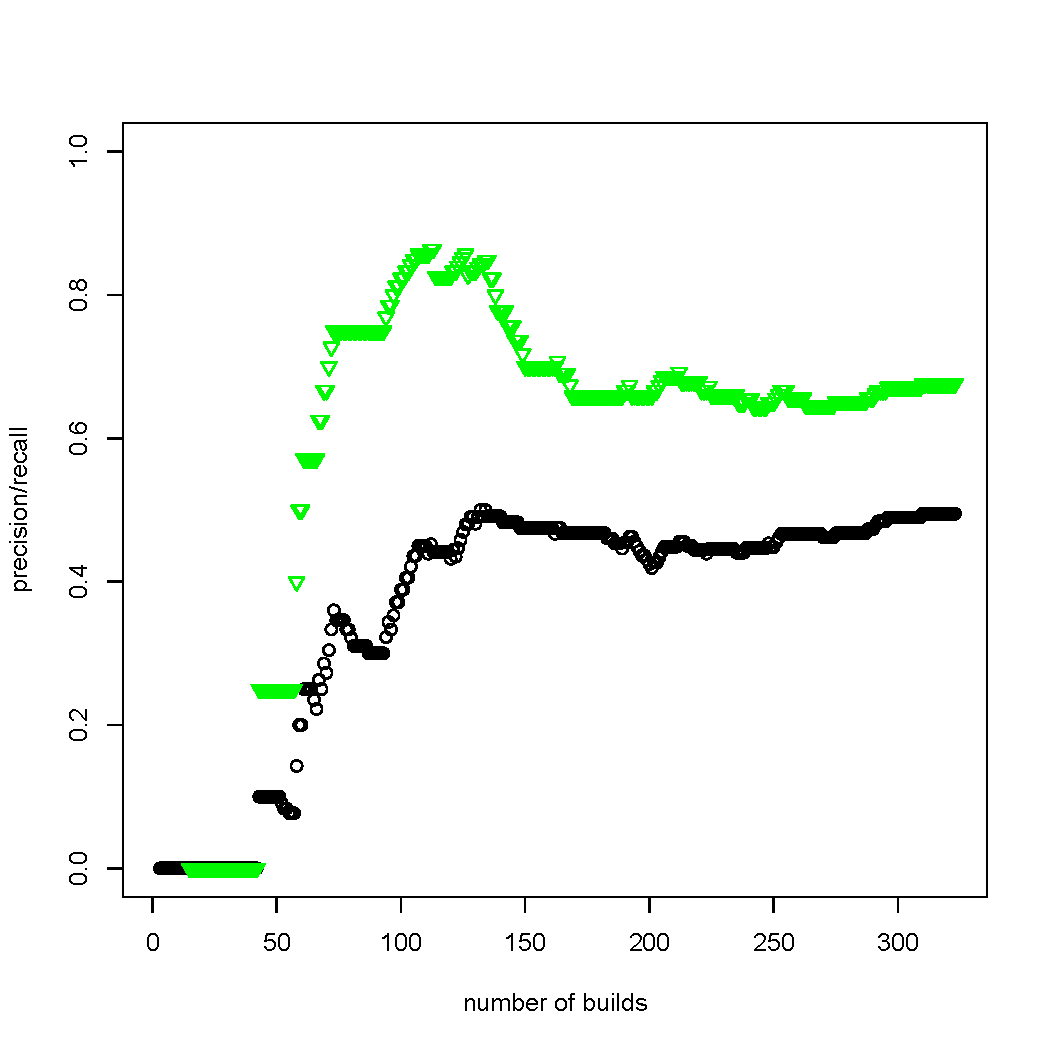
\includegraphics[width=\columnwidth]{figures/precission-recall}
\label{fig:prediction-svm}
}
\subfloat[Evaluation results from the Logistic Regression.] {
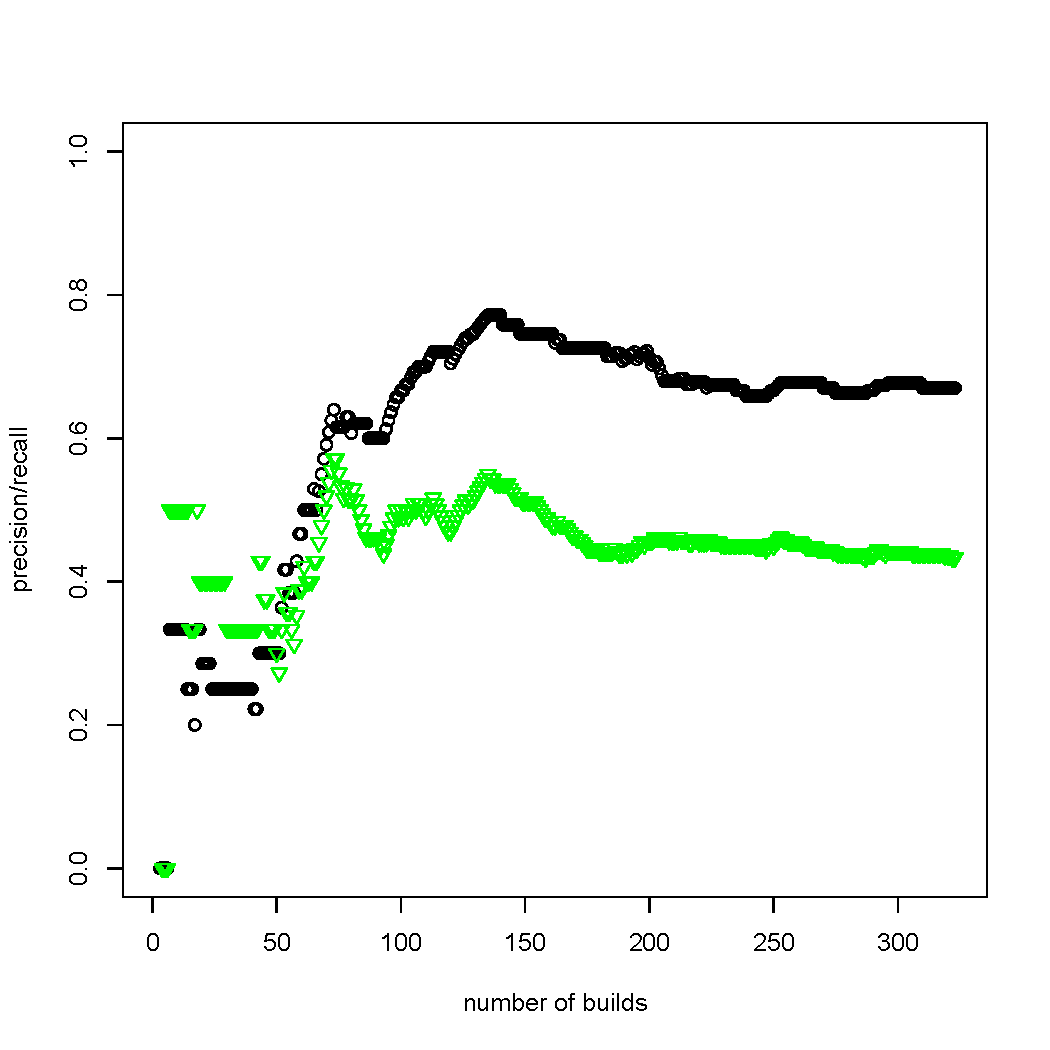
\includegraphics[width=\columnwidth]{figures/precision-recall-logreg}
\label{fig:prediction-logreg}
}
\caption{Plotting the precision (green downward pointing triangles) and recall (black hollow circles) of the support vector machine (left) and the logistic regression (right).}
\label{fig:prediction}
\end{figure*}

\section{Build Failure Prediction}
\label{sec:prediction}
To answer our first research question, we build a predictive model that uses the
constructed socio-technical networks as input to predict whether a build succeeds
or fails. Since we are interested in the practical application of this model we
diverge from the standard evaluation tactic and use a more practical relevant
approach. After we presente the results of our prediction model we discuss their
implications.

\subsection{Model Evaluation}
We train several prediction models, such as logistic regression, support vector
machines, decision trees, and a bayesian classifiers, using features we
extract from the constructed socio-technical networks. Each feature represents a pair of
connected developers in the network and the type of the edge that they are
connected with (i.e. social, technical or socio-technical).

%To evaluate those model, we take a more practical evaluation approach.
To accomplish a more practical evaluation, we order all our social networks by the time the build they were constructed from was tested.
Having the networks ordered according to build time we evaluate our prediction model in the following five steps:%\todo{make pictures}

\begin{enumerate}
\item Get the first $n$ networks and perform a principle component analysis on the extracted features.
\item Select the principal components that explain the most variance until 95\% of the total variance of the training set can be explained.
%\item Determine the principal components of the first $n$ networks.
\item Train the model using the principal components of the first $n$ networks.
\item Test the model on network $n+1$ after transforming it to the determined principal components.
\item Increase $n$ by 1 and repeat until $n+1$ is the size of complete data set.
\end{enumerate}

This evaluation technique is meant to simulate the actual usage of the prediction model.
In software practice builds come in one by one.
This means that whenever a build has been verified the model can be extended using the social network from the newest build for training. 
This method of evaluation is closer to the actual usage in the field than
random splits or cross validation.

We used two coefficients to assess the models quality at any given time: recall (Eq.~\ref{eq:recall}) and precision (Eq.~\ref{eq:precision}).
The recall of a model describes the percentage of how many failed builds where predicted correctly.
This translates into the formula:

\begin{equation}
\label{eq:recall}
\text{recall}=\frac{\text{Correctly \emph{as failed} Predicted Builds}}{\text{All Failed Builds}}
\end{equation}

Precision on the other hand describes the percentage of how many of the \emph{as failed} predicted builds are actually failed builds. Thus we can express precision using the following formula:

\begin{equation}
\label{eq:precision}
\text{precision}=\frac{\text{Correctly \emph{as failed} Predicted Builds}}{\text{All \emph{as failed} Predicted Builds}}
\end{equation}

Both recall and precision lie in the interval from 0 to 1, with 1 being best and 0 being worst.
We compute the recall and precision for each iteration by accumulating the prediction results of all previous prediction results.
For example if we went through 20 iterations we create a contingency table from the predicted results for the last 20 builds.
Each prediction can have one of four outcomes: (1) correctly predicted \emph{as failed}, (2) correctly predicted as succeeded, (3) falsely predicted \emph{as failed}, and (4) falsely predicted as succeeded.
Adding those numbers till the most recent prediction enables us to compute precision and recall.


The current standard evaluation for failure prediction models in software engineering is to take the data set and generate a number of random splits (e.g.~\cite{zimmermann:icse:2008,schroeter:isese:2006,nagappan:icse:2008}).
A random split partitions the data into a training and a testing data set, where the model is trained with the training data and then evaluated using the testing set.
Other also used cross validation which creates $n$ partitions and tests with each partition while training with the remaining $n-1$ partitions (e.g.~\cite{wolf:icse:2009}).

Although random splits and cross validation allow for a random combination, they completely ignore the explicit order.
This leads to the problem that random splits and cross validation allow features that might emerge later and should not have been available to be used for training.
For example, if a developer joins the project after it started, she cannot have been present in any of the networks previous to her date of joining the project.
This means that the model at first cannot use any information about her connections to others.

%%%%%%%%%%%%%%%%%%%%%%%%%%%%%%%



\subsection{Results}
Of the prediction models we evaluated, we present the results for the support
vector machine and the logistical regression. The support vector machine produced
the best results whereas the logistical regression serves as comparison to the
support vector machine results as well as indicating the reliability of
the regression analysis presented later in Section~\ref{sec:pattern}.

% describe support vector machine \todo{talk about three sections of the figures}
Figure~\ref{fig:prediction} shows the recall and precision values for the
suport vector machine and the logistical regression models. The green downward
pointing triangles represent the precision of the model for each iteration, note that we started training each model with at least three data points. The black circles represent the recall of a model for each
iteration.

Both Subfigures in Figure~\ref{fig:prediction} can be divided into three
sections. The first section is comprised of the first 70-80 iterations where,
by a manual investigation, we observe that the support vector machine predicts almost everything to be successful in contrast to the unstable logistic regression.

The middle section is characterized by a peek efficiency between 100 and 150
iterations in both prediction models. Before that peak both models underperform, where the support vector machine suffers more than the logistic regression from a small data set.

In the last segment after 150-180 iteration the precision and recall values
stabilize over both models. In contrast to the logistic regression the support vector machine obtains a higher precision and a lower recall with a slight upward trend.
The support vector machine ended with a precision of $.68$ (median: $.67$) and a recall of $.49$ (median: $.45$) whereas the logistic regression obtained a precision and recall value of $.43$ (median: $.45$) and $.67$ (median: $.67$) respectively.












\subsection{Discussion}
% - why did we fulfill our objective
Although the overall performance of the models is not yet practical due to low
precision and recall, these results are interesting. On the one hand, we consider
answering our first research question with yes: we can use developer pairs to
predict build failure. We consider the model to be sufficient because we, as Wolf
et al.~\cite{wolf:icse:2009}, outperform a random guess which would have
resulted in both recall and precision of less than $.33$, which is the percentage of failed
builds. To our knowledge there have been only two studies that focused on
predicting build outcomes: by Hassan et al.~\cite{hassan:ase:2006} and by Wolf et
al.~\cite{wolf:icse:2009}. Our approach places itself between the results of both
studies with our study being better than results obtained by Wolf et
al.~\cite{wolf:icse:2009} but being worse than Hassans et
al.~\cite{hassan:ase:2006} approach.

Despite of outperforming the random guess the precision of our models is of concern because
it indicates the rate at which we falsely report a build to fail. With a median
 precision of $.67$, every third of the \emph{as failed} build predicted by the support
 vector machine would be a false positive. Besides the low trust a developer
 can develop in the model, it also reports less than half of the failed builds
 as failed.


% - why is the beginning so weak
We provide some possible explanations here. In the first part of the
Figures~\ref{fig:prediction-svm} and~\ref{fig:prediction-logreg}, we observed
that all models perform poorly as long as they have less than 100 builds to train
on. After investigating the first 100 builds we found that new
developers are continually appearing in the development pairs. This means that
prediction models need to make predictions without having enough knowledge to
train on, thus resorting to predict the build to be the most likely outcome, to be OK.

%- check peeks with respect to new developers entering the team
A peak in the interval of 100-150 iterations occurred in both models for both recall and precision.
Within this interval the team changed and new people joined the project and people where reallocated to work on new functionality which meant creating new dependencies and leaving old dependencies behind.
This change in dependencies confused the model in a way that it did not perform as well.
Both models stabilize over time with the support vector machine exhibiting a slight upward trend.

% - what is the next step
Since the goal of this research is to find a way to create actionable knowledge
to avoid build failure, building a prediction model was the first step to show
that developer pairs have an effect on the actual prediction. The results from
the prediction models is first evidence that developer relationships have an
influence on the build. Next we continue with perusing our second research
question that examined the relationship between particular developer
pairs (i.e. technical pairs) and build results. This will help us
investigate how we might prevent builds from failing by changing the
nature of developer relations in these pairs.





\begin{table}[t]
\centering%\vspace{1cm}
\begin{tabular}{rcc}
\toprule
 & successful & failed  \\
 \midrule
(Adam, Bart) & 3 & 13 \\
$\neg$ (Adam, Bart) & 224 & 86\\
\midrule
total&227&99\\\bottomrule
%User3493, User2943 & 3 & 13
\end{tabular}
\caption{Contingency table for technical pair (Adam, Bart) in relation to build
success or failure}
\label{tab:contingencytable}
\end{table}



\addtocounter{table}{1}
\begin{table*}[t]
\centering
\subfloat[Twenty most frequent \emph{technical pairs} that are failure-related.]{
\begin{tabular}{@{\hspace{.2cm}}ccc@{\hspace{.75cm}}c@{\hspace{.2cm}}}
\toprule
Pair & \#successful & \#failed & $p_x$\\
\midrule
%Cody-Daisy&  0 & 12 & 1.0000 \\
%Adam-Ina & 0 & \phantom{1}8 & 1.0000 \\
%Adam-Kim& 0 & \phantom{1}8 & 1.0000 \\
%Adam-Nina & 0 & \phantom{1}6 & 1.0000 \\
%Fred-Gina& 0 & \phantom{1}6 & 1.0000 \\
%Gina-Oliver & 0 & \phantom{1}6 & 1.0000 \\
%Adam-Daisy& 1 & 14 & 0.9720\\%67 \\
%Bart-Daisy& 1 & \phantom{1}9 & 0.9572\\%127 \\
%Adam-Lisa& 1 & \phantom{1}8 & 0.9521\\%204 \\
%Bart-Eve & 2 & 11 & 0.9318\\%403 \\
%\textbf{Adam}-\textbf{Bart}& \textbf{3} & \textbf{13} & \textbf{0.9150}\\%485 \\
%Bart-Cody & 3 & 13 & 0.9150\\%485 \\
%Adam-Eve & 4 & 16 & 0.9086\\%162 \\
%Daisy-Ina & 3 & 12 & 0.9086\\%162 \\
%Cody-Fred& 3 & 10 & 0.8923\\%077 \\
%Bart-Herb & 3 & 10 & 0.8923\\%077 \\
%Cody-Eve & 5 & 15 & 0.8817\\%568 \\
%Adam-Jim & 4 & 11 & 0.8723\\%792 \\
%Herb-Paul & 5 & 12 & 0.8564\\%397 \\
%Mike-Rob& 6 & 13 & 0.8434\\%004\\
%Adam-Fred & 6 & 13 & 0.8434\\%004\\
%
%User11137, User4105 & 0 & 12 & 1.0000 \\
%User2943, User13877 & 0 & 8 & 1.0000 \\
%User7438, User2943 & 0 & 8 & 1.0000 \\
%User2943, User2810 & 0 & 6 & 1.0000 \\
%User8645, User1976 & 0 & 6 & 1.0000 \\
%User8645, User2267 & 0 & 6 & 1.0000 \\
%User11137, User2943 & 1 & 14 & 0.9675\\%908 \\
%User11137, User3493 & 1 & 9 & 0.9504\\%773 \\
%User6012, User2943 & 1 & 8 & 0.9446\\%298 \\
%User3493, User2435 & 2 & 11 & 0.9214\\%387 \\
%User3493, User2943 & 3 & 13 & 0.9023\\%53 \\
%User3493, User4105 & 3 & 13 & 0.9023\\%53 \\
%User2943, User2435 & 4 & 16 & 0.8950\\%695 \\
%User11137, User13877 & 3 & 12 & 0.8950\\%695 \\
%User1976, User4105 & 3 & 10 & 0.8766\\%716 \\
%User3493, User6339 & 3 & 10 & 0.8766\\%716 \\
%User4105, User2435 & 5 & 15 & 0.8648\\%208 \\
%User2943, User9017 & 4 & 11 & 0.8543\\%22 \\
%User6339, User13875 & 5 & 12 & 0.8365\\%498 \\
%User10979, User3385 & 6 & 13 & 0.8220\\%793\\
%User2943, User1976 & 6 & 13 & 0.8220\\%793 \\
%
(Cody, Daisy)	&	0&	12&	1		\\ %user11137.user4105.T
(Adam, Daisy)	&	1&	14&	0.9697	\\ %user11137.user2943.T
(Bart, Eve)	&	2&	11&	0.9265	\\ %user3493.user2435.T
(Adam, Bart)	&	3&	13&	0.9085	\\ %user3493.user2943.T
(Bart, Cody)	&	3&	13&	0.9085	\\ %user3493.user4105.T
(Adam, Eve)	&	4&	16&	0.9016	\\ %user2943.user2435.T
(Daisy, Ina)	&	3&	12&	0.9016	\\ %user11137.user13877.T
(Cody, Fred)	&	3&	10&	0.8843	\\ %user1976.user4105.T
(Bart, Herb)	&	3&	10&	0.8843	\\ %user3493.user6339.T
(Cody, Eve)	&	5&	15&	0.8730	\\ %user4105.user2435.T
(Adam, Jim)	&	4&	11&	0.8631	\\ %user2943.user9017.T
(Herb, Paul)	&	5&	12&	0.8462	\\ %user6339.user13875.T
(Cody, Fred)	&	5&	11&	0.8345	\\ %user11137.user1976.T
(Mike, Rob)	&	6&	13&	0.8324	\\ %user10979.user3385.T
(Adam, Fred)	&	6&	13&	0.8324	\\ %user2943.user1976.T
(Daisy, Fred)	&	8&	13&	0.7884	\\ %user3493.user1976.T
(Gill, Eve)		&	7&	10&	0.7661	\\ %user1264.user2435.T
(Daisy, Ina)	&	7&	10&	0.7661	\\ %user3493.user13873.T
(Fred, Ina)	&	8&	10&	0.7413	\\ %user1976.user13877.T
(Herb, Eve)	&	8&	10&	0.7413	\\ %user6339.user2435.T
\bottomrule
\end{tabular}
%\caption{Twenty \emph{technical pairs} that are failure-related and affect the most builds.}
\label{tab:badtechpairs}
}\hspace{1.3cm}
%\end{table}
%
\subfloat[The twenty corresponding \emph{socio-technical pairs}, which are not statistically related to failed builds.]{
\begin{tabular}{@{\hspace{.2cm}}ccc@{\hspace{.75cm}}c@{\hspace{.2cm}}}
\toprule
Pair & \#successful & \#failed & $p_x$ \\
\midrule
(Cody, Daisy)	&	---&	---&	---\\
(Adam, Daisy)	&	---&	---&	---\\
(Bart, Eve)	&	1&	4&	0.9016\\
(Adam, Bart)	&	---&	---&	---\\
(Bart, Cody)	&	---&	---&	---\\
(Adam, Eve)	&	---&	---&	---\\
(Daisy, Ina)	&	---&	---&	---\\
(Cody, Fred)	&	1&	0&	0\\
(Bart, Herb)	&	1&	2&	0.8209\\
(Cody, Eve)	&	0&	3&	1\\
(Adam, Jim)	&	0&	1&	1\\
(Herb, Paul)	&	1&	0&	0\\
(Cody, Fred)	&	---&	---&	---\\
(Mike, Rob)	&	---&	---&	---\\
(Adam, Fred)	&	---&	---&	---\\
(Daisy, Fred)	&	---&	---&	---\\
(Gill, Eve)		&	---&	---&	---\\
(Daisy, Ina)	&	1&	0&	0\\
(Fred, Ina)	&	0&	2&	1\\
(Herb, Eve)	&	---&	---&	---\\
\bottomrule
\end{tabular}
%\caption{Twenty \emph{technical pairs} that are failure-related and affect the most builds.}
\label{tab:stechpairs}
}
\caption{The 20 most frequent statistically failure related technical pairs and the corresponding socio-technical pairs.}
\label{tab:pairs}
\end{table*}
\addtocounter{table}{-1}




% \section{Pattern Analysis}
\section{Which Pairs Induce Failure?}
\label{sec:pattern}
In this section we answer our second research question, ``Are there
developer technical pairs that influence the build outcome?''. 
We first explain our analysis approach followed by the results obtained and a
short discussion of the results.

\subsection{Analysis of Socio-Technical Gaps}
The lack of communication between two developers that share a
technical dependency is referred to in the literature as a
socio-technical gap~\cite{valetto:msr:2007}. Because research suggests negative influence of such gaps, we are interested in analyzing pairs of developers that share a technical edge (implying coordination need) but no social edge (implying
unmet coordination need) in socio-technical networks. We refer to these pairs of
developers as \emph{technical pairs} (there is a gap), and to those that do
share a socio-technical edge (there is no gap) as \emph{socio-technical pairs}. 

To answer our second research question, we analyze the
technical pairs in relation to build
failure. Our analysis proceeds in four steps:

\begin{enumerate}
\item Identify all technical pairs from the socio-technical networks.
\item For each technical pair count occurrences in socio-technical networks of
failed builds.
\item For each technical pair count occurrences in socio-technical networks of
successful builds.
\item Determine if the pair is significantly related to success or failure.
\end{enumerate}

For example, in Table~\ref{tab:contingencytable} we illustrate the analysis of
the technical pair (Adam, Bart). This pair appears in 3 successful builds and in
13 failed builds. Thus it does not appear in 224 successful builds, which is the total number of successful builds minus the number of successful builds the pair appeared in, and it is absent in 86 failed builds.
A Fischer Exact Value test yields significance at a confidence level of $\alpha = .05$ with a p-value of $4.273\cdot10^{-5}$.

Note that we adjust the p-values of the Fischer Exact Value test to account for multiple hypothesis testing using the Bonferroni adjustment.
The adjustment is necessary because we deal with 961 technical pairs that need to be tested. 

To enable us to discuss the findings as to whether closing socio-technical gaps
are needed to avoid build failure, or which of these gaps are more important to
close, we peform two additional analyses. 
First we analyze whether the
socio-technical pairs also appear to be build failure-related or not, by
following the same steps as above for socio-technical pairs. 
%
Secondly, we prioritize the developer pairs using the coefficient $p_x$,
which represents the normalized likelihood of a build
to fail in the presence of the specific pair:

\begin{equation}
p_x\text{=}\frac{ \text{pair}_{failed} / \text{total}_{failed} }
                     { \text{pair}_{failed} / \text{total}_{failed} + \text{pair}_{success} / \text{total}_{successs}}
\end{equation}

The coefficient is comprised of four counts: (1) pair$_{failed}$, the number of failed builds where the pair occurred; (2) total$_{failed}$, the number of failed builds; (3) pair$_{success}$, the number of successful builds where the pair occurred; (4) total$_{success}$, the number of successful builds.
%This coefficient is normalized with the number of failed and successful builds.
A value closer to one means that the developer pair is strongly related to build
failure. %Additionally it describes a probability of failure likelihood that accounts for the imbalance in the data.




\addtocounter{table}{1}
\begin{table}[t]
\centering
\begin{tabular}{cccc}
\toprule
Feature & Coefficient & p-value & \\
\midrule
%(Intercept)             &  7.897e+74 & 3.743e+09 &  2.110e+65  &  <2e-16 & ***\\
%\\
%user11137.user4105.T    &   -5.669e+75  & 2.421e+10 &-2.342e+65 &  <2e-16 & ***\\
%user11137.user2943.T    &   -9.846e+75  &  7.788e+09 &-1.264e+66  & <2e-16 &***\\
%user3493.user2435.T      &    -1.258e+75      & 3.477e+10  &3.619e+64   &<2e-16 &***\\
%user3493.user2943.T      &    -1.605e+76     & 5.427e+10  &2.958e+65  & <2e-16 &***\\
%user3493.user4105.T      &   -3.419e+76     & 3.837e+10 &-8.910e+65  & <2e-16 &***\\
%user2943.user2435.T      &    -2.610e+76      & 2.966e+10  &8.801e+65  & <2e-16 &***\\
%user11137.user13877.T  &  -8.105e+74   & 3.036e+10 &-2.669e+64 &  <2e-16 &***\\
%user1976.user4105.T      &    -5.348e+76     & 2.359e+10  &2.267e+66   &<2e-16 &***\\
%user3493.user6339.T      &   -2.977e+76    &1.028e+11 &-2.895e+65   &<2e-16 &***\\
%user4105.user2435.T      &   -2.315e+76   & 1.618e+10 &-1.431e+66  & <2e-16 &***\\
%user2943.user9017.T      &    -2.724e+76    &2.621e+10  &1.039e+66  & <2e-16 &***\\
%user6339.user13875.T    &   -1.636e+76   & 4.081e+08 &-4.010e+67   &<2e-16 &***\\
%user11137.user1976.T    &   -1.645e+74   &4.024e+09 &-4.087e+64  & <2e-16 &***\\
%user10979.user3385.T    &    -1.327e+75   &3.668e+09  &3.619e+65  & <2e-16 &***\\
%user2943.user1976.T      &   -5.250e+76   &1.269e+10 &-4.136e+66  & <2e-16 &***\\
%user3493.user1976.T      &   -2.455e+75   & 3.523e+10 &-6.970e+64   &<2e-16 &***\\
%user1264.user2435.T      &    -7.162e+75   &3.589e+09  &1.996e+66  & <2e-16 &***\\
%user3493.user13873.T    &   -5.325e+74   & 3.464e+10 &-1.537e+64   &<2e-16 &***\\
%user1976.user13877.T    &    -2.777e+75   & 7.334e+08  &3.786e+66  & <2e-16 &***\\
%user6339.user2435.T      &    -1.799e+75   & 1.584e+09  &1.136e+66  & <2e-16 &***\\
%\\
%\#Change Sets per Build      & \phantom{-}6.480e+60 & 8.539e+06 & 7.589e+53 &  <2e-16 &***\\
%\#Files changed per Build             &-4.530e+60 & 3.072e+06 &-1.475e+54  & <2e-16 &***\\
%{\small \#Developers contributed per Build}  &   \phantom{-}3.386e+61 & 2.687e+07 & 1.260e+54 &  <2e-16 &***\\
%\#Work Items per Build     &  -3.690e+61 & 1.859e+07 &-1.984e+54  & <2e-16 &***\\
%
(Intercept)            &  7.897e+74 &  <2e-16 & ***\\
\\
(Cody, Daisy)  &  	-5.669e+75  &  <2e-16 & ***\\
(Adam, Daisy)  &   -9.846e+75  &   <2e-16 &***\\
(Bart, Eve)  	&   -1.258e+75  &<2e-16 &***\\
(Adam, Bart)  	&   -1.605e+76  & <2e-16 &***\\
(Bart, Cody)  	&   -3.419e+76  & <2e-16 &***\\
(Adam, Eve)  	&   -2.610e+76  & <2e-16 &***\\
(Daisy, Ina)  	&  	-8.105e+74 	 &  <2e-16 &***\\
(Cody, Fred)  	&   -5.348e+76  &<2e-16 &***\\
(Bart, Herb)  	&   -2.977e+76  &<2e-16 &***\\
(Cody, Eve)  	&   -2.315e+76  & <2e-16 &***\\
(Adam, Jim)  	&   -2.724e+76    & <2e-16 &***\\
(Herb, Paul)  	&   -1.636e+76      &<2e-16 &***\\
(Cody, Fred)  	&   -1.645e+74     & <2e-16 &***\\
(Mike, Rob)  	&   -1.327e+75    & <2e-16 &***\\
(Adam, Fred)  	&   -5.250e+76     & <2e-16 &***\\
(Daisy, Fred)  &   -2.455e+75      &<2e-16 &***\\
(Gill, Eve)	  	&   -7.162e+75    & <2e-16 &***\\
(Daisy, Ina)  	&   -5.325e+74      &<2e-16 &***\\
(Fred, Ina)  	&   -2.777e+75     & <2e-16 &***\\
(Herb, Eve)  	&   -1.799e+75     & <2e-16 &***\\
\\
\#Change Sets per Build     & \phantom{-}6.480e+60 &   <2e-16 &***\\
\#Files changed per Build            &-4.530e+60 &  <2e-16 &***\\
{\small \#Developers contributed per Build}  &   \phantom{-}3.386e+61 &  <2e-16 &***\\
\#Work Items per Build    &  -3.690e+61   & <2e-16 &***\\
%
%
%
%user6012.user2943.T     -1.198e+76  1.415e+10 -8.466e+65   <2e-16 ***\\
%user11137.user3493.T     4.917e+76  2.255e+10  2.180e+66   <2e-16 ***\\
%user2943.user13877.T    -2.086e+76  3.598e+10 -5.796e+65   <2e-16 ***\\
%user8645.user1976.T     -1.172e+75  4.535e+09 -2.585e+65   <2e-16 ***\\
%user8645.user2267.T      1.358e+76  2.934e+10  4.628e+65   <2e-16 ***\\
%user7438.user2943.T      1.562e+75  2.562e+10  6.096e+64   <2e-16 ***\\
%user10761.user9609.T    -1.244e+68  1.972e+08 -6.307e+59   <2e-16 ***\\
%user11208.user9017.T    -7.661e+73  6.520e+07 -1.175e+66   <2e-16 ***\\
%user11137.user8543.T    -7.938e+74  1.813e+08 -4.378e+66   <2e-16 ***\\
%user11281.user8543.T     1.520e+75  3.323e+09  4.573e+65   <2e-16 ***\\
%user3818.user8543.T     -1.655e+75  2.732e+10 -6.058e+64   <2e-16 ***\\
%user13877.user8543.T     1.802e+74  3.352e+09  5.377e+64   <2e-16 ***\\
%user9017.user13871.T    -3.613e+74  6.052e+09 -5.970e+64   <2e-16 ***\\
%user8645.user11281.T    -6.742e+73  1.058e+08 -6.371e+65   <2e-16 ***\\
%user2983.user9017.T     -6.303e+73  8.157e+09 -7.727e+63   <2e-16 ***\\
%user10979.user13875.T    1.507e+75  1.803e+10  8.355e+64   <2e-16 ***\\
%user9017.user13874.T    -2.791e+76  1.140e+11 -2.450e+65   <2e-16 ***\\
%user1264.user13874.T    -8.654e+75  2.838e+10 -3.049e+65   <2e-16 ***\\
%user3493.user9017.T     -2.786e+75  4.274e+09 -6.519e+65   <2e-16 ***\\
%user4105.user13874.T     1.206e+76  9.252e+10  1.303e+65   <2e-16 ***\\
%user2943.user13871.T    -6.665e+75  3.166e+10 -2.105e+65   <2e-16 ***\\
%user9017.user1976.T     -1.910e+63  3.850e+09 -4.960e+53   <2e-16 ***\\
%user10979.user2435.T     6.269e+63  3.579e+09  1.752e+54   <2e-16 ***\\
%user6639.user6339.T      3.075e+64  2.102e+10  1.463e+54   <2e-16 ***\\
%user6012.user9017.T     -5.463e+63  3.603e+09 -1.516e+54   <2e-16 ***\\
%user6339.user4105.T      5.169e+63  3.628e+09  1.425e+54   <2e-16 ***\\
%user9172.user2435.T     -1.212e+63  1.626e+09 -7.453e+53   <2e-16 ***\\
%user7438.user8543.T      5.042e+62  1.641e+09  3.073e+53   <2e-16 ***\\
%user11137.user13871.T    6.266e+62  5.193e+08  1.207e+54   <2e-16 ***\\
%user10979.user11281.T   -5.506e+63  3.719e+09 -1.480e+54   <2e-16 ***\\
%user11137.user6012.T     2.332e+63  1.532e+09  1.522e+54   <2e-16 ***\\
%user11137.user13874.T   -1.913e+64  1.393e+10 -1.373e+54   <2e-16 ***\\
%user1264.user4105.T      1.212e+63  1.420e+09  8.533e+53   <2e-16 ***\\
%user8645.user6096.T      6.633e+63  4.523e+09  1.467e+54   <2e-16 ***\\
%user11281.user9609.T     5.157e+62  7.503e+07  6.873e+54   <2e-16 ***\\
%user13871.user4163.C     8.406e+61  1.717e+08  4.897e+53   <2e-16 ***\\
%user11840.user9172.C    -1.672e+61  4.148e+08 -4.031e+52   <2e-16 ***\\
%user11840.user9983.C     2.743e+62  2.898e+08  9.463e+53   <2e-16 ***\\
%user6727.user9983.C      1.659e+63  1.698e+09  9.771e+53   <2e-16 ***\\
%user11208.user6727.C    -2.455e+63  1.596e+09 -1.538e+54   <2e-16 ***\\
%user3057.user13873.C     1.983e+62  1.260e+08  1.574e+54   <2e-16 ***\\
%user11137.user11208.C   -9.030e+61  2.237e+08 -4.036e+53   <2e-16 ***\\
%user3982.user6012.C     -2.567e+62  3.356e+08 -7.648e+53   <2e-16 ***\\
%user3818.user10979.C     1.868e+62  1.228e+08  1.522e+54   <2e-16 ***\\
%user6012.user9172.C      1.353e+62  1.089e+08  1.242e+54   <2e-16 ***\\
%user13877.user13875.C   -1.013e+63  6.884e+08 -1.472e+54   <2e-16 ***\\
%user11208.user7438.C     8.180e+61  8.746e+07  9.353e+53   <2e-16 ***\\
%user10979.user6096.C    -5.291e+63  3.648e+09 -1.450e+54   <2e-16 ***\\
%user6096.user7395.C     -3.135e+61  1.839e+08 -1.705e+53   <2e-16 ***\\
%user4105.user5275.C      2.725e+63  9.779e+08  2.787e+54   <2e-16 ***\\
%user7146.user4163.C      1.171e+63  5.291e+08  2.214e+54   <2e-16 ***\\
%user11208.user2267.C     3.459e+61  3.525e+08  9.813e+52   <2e-16 ***\\
%user7224.user4163.C      2.375e+61  1.379e+08  1.723e+53   <2e-16 ***\\
%user13877.user2435.C     2.353e+63  1.838e+09  1.280e+54   <2e-16 ***\\
%user6012.user7146.C     -6.092e+62  2.884e+08 -2.112e+54   <2e-16 ***\\
%user2983.user7224.C      2.961e+61  1.340e+08  2.209e+53   <2e-16 ***\\
%user13235.user1976.C     7.225e+63  5.490e+09  1.316e+54   <2e-16 ***\\
%user11208.user7372.C     5.809e+63  3.983e+09  1.458e+54   <2e-16 ***\\
%user13235.user13874.C    5.605e+63  3.718e+09  1.507e+54   <2e-16 ***\\
%user3057.user13874.C     5.278e+63  3.817e+09  1.383e+54   <2e-16 ***\\
%user11208.user6012.C     4.458e+61  1.043e+08  4.273e+53   <2e-16 ***\\
%user7002.user2020.C     -5.853e+63  3.978e+09 -1.471e+54   <2e-16 ***\\
%user2744.user11208.C     7.773e+62  7.092e+08  1.096e+54   <2e-16 ***\\
%user9172.user5275.C      1.397e+64  9.128e+09  1.530e+54   <2e-16 ***\\
%user6677.user7224.C      2.952e+61  1.316e+08  2.244e+53   <2e-16 ***\\
%user3818.user6639.C      5.573e+61  2.800e+08  1.991e+53   <2e-16 ***\\
%user7002.user4105.C     -2.017e+63  9.206e+08 -2.191e+54   <2e-16 ***\\
%user12149.user2943.C    -1.655e+64  9.635e+09 -1.718e+54   <2e-16 ***\\
%user7438.user7372.C     -9.768e+61  2.375e+08 -4.113e+53   <2e-16 ***\\
%user4955.user2306.C     -4.290e+62  4.334e+08 -9.898e+53   <2e-16 ***\\
%user11137.user7438.C    -8.275e+61  7.426e+08 -1.114e+53   <2e-16 ***\\
%user11208.user7002.C     1.709e+62  8.605e+07  1.986e+54   <2e-16 ***\\
%user3057.user1976.C      3.156e+60  4.486e+08  7.034e+51   <2e-16 ***\\
%user3982.user4163.C     -1.497e+63  7.778e+08 -1.925e+54   <2e-16 ***\\
%user10761.user4105.C     5.332e+62  3.087e+08  1.727e+54   <2e-16 ***\\
%user7438.user6639.C     -4.700e+62  1.319e+08 -3.564e+54   <2e-16 ***\\
%user10761.user6339.C     8.421e+61  1.068e+08  7.887e+53   <2e-16 ***\\
%user7438.user2267.C      5.206e+62  8.470e+07  6.146e+54   <2e-16 ***\\
%user11840.user2267.C    -1.418e+62  3.676e+08 -3.858e+53   <2e-16 ***\\
%user3057.user4163.C      5.427e+63  3.853e+09  1.409e+54   <2e-16 ***\\
%user11208.user6639.C     6.044e+62  6.502e+08  9.295e+53   <2e-16 ***\\
%user6012.user4163.C      4.410e+61  9.535e+07  4.625e+53   <2e-16 ***\\
%user6677.user6379.C      1.691e+61  1.481e+08  1.142e+53   <2e-16 ***\\
%user10761.user3639.C    -1.635e+62  1.878e+08 -8.709e+53   <2e-16 ***\\
%user9655.user10979.C    -1.393e+61  8.225e+07 -1.693e+53   <2e-16 ***\\
%user4955.user9986.TC     5.594e+61  8.556e+07  6.538e+53   <2e-16 ***\\
%user4105.user1567.C      1.454e+62  9.109e+07  1.596e+54   <2e-16 ***\\
%user9609.user6012.T      5.290e+61  1.824e+08  2.900e+53   <2e-16 ***\\
%user11281.user2267.T    -5.499e+63  3.725e+09 -1.476e+54   <2e-16 ***\\
%user2983.user8860.C      3.596e+62  1.531e+08  2.349e+54   <2e-16 ***\\
%user3672.user13875.C    -6.807e+61  1.880e+08 -3.621e+53   <2e-16 ***\\
%user2452.user9983.C     -3.179e+62  3.396e+08 -9.359e+53   <2e-16 ***\\
%user3756.user7372.C      7.300e+61  5.508e+07  1.325e+54   <2e-16 ***\\
%user3539.user13877.C     4.104e+62  1.941e+08  2.114e+54   <2e-16 ***\\
%user2460.user6103.C      8.697e+61  3.716e+08  2.340e+53   <2e-16 ***\\
%user6021.user9017.C      1.049e+62  7.032e+07  1.491e+54   <2e-16 ***\\
%user6901.user2038.T      2.862e+61  9.837e+07  2.909e+53   <2e-16 ***\\
%user6677.user5963.C      9.236e+60  7.371e+07  1.253e+53   <2e-16 ***\\
%user10761.user6677.C    -4.323e+62  4.038e+08 -1.071e+54   <2e-16 ***\\
%user13874.user11208.C   -5.371e+63  3.581e+09 -1.500e+54   <2e-16 ***\\
%user3982.user2943.C     -6.644e+61  2.197e+08 -3.024e+53   <2e-16 ***\\
%user3057.user7286.C     -2.138e+60  1.090e+08 -1.962e+52   <2e-16 ***\\
%user7111.user11623.C     1.263e+63  5.111e+08  2.471e+54   <2e-16 ***\\
%user9983.user6677.C      3.487e+62  3.489e+08  9.995e+53   <2e-16 ***\\
%user7438.user6677.TC    -5.068e+63  3.650e+09 -1.388e+54   <2e-16 ***\\
%user11281.user7438.C     2.607e+61  9.562e+07  2.726e+53   <2e-16 ***\\
%user4686.user6391.C      3.592e+62  1.623e+08  2.214e+54   <2e-16 ***\\
%user10303.user4105.C     9.159e+61  7.919e+07  1.157e+54   <2e-16 ***\\
%user4955.user3818.C      1.993e+62  1.600e+08  1.246e+54   <2e-16 ***\\
%user13871.user6391.C    -1.917e+62  2.296e+08 -8.351e+53   <2e-16 ***\\
%user11137.user3818.T    -1.882e+62  1.920e+08 -9.800e+53   <2e-16 ***\\
%user9609.user11281.TC   -1.094e+62  1.955e+08 -5.596e+53   <2e-16 ***\\
%user6677.user6639.C     -4.807e+63  3.646e+09 -1.319e+54   <2e-16 ***\\
%user7689.user7286.C      2.220e+60  7.506e+07  2.958e+52   <2e-16 ***\\
%user7438.user7689.T     -1.661e+62  1.214e+08 -1.368e+54   <2e-16 ***\\
%user6677.user2810.C     -2.554e+60  6.772e+07 -3.771e+52   <2e-16 ***\\
%user1077.user13871.C    -1.468e+61  8.322e+07 -1.764e+53   <2e-16 ***\\
%user11208.user13871.T   -6.376e+61  1.523e+08 -4.187e+53   <2e-16 ***\\
%user6639.user11281.C    -1.021e+62  8.631e+07 -1.183e+54   <2e-16 ***\\
%user6677.user6727.C     -8.135e+61  1.169e+08 -6.959e+53   <2e-16 ***\\
%user10761.user1264.C    -9.014e+60  2.694e+08 -3.346e+52   <2e-16 ***\\
%user2452.user2983.C      6.650e+61  9.949e+07  6.685e+53   <2e-16 ***\\
%user11281.user7438.TC    2.085e+62  7.164e+07  2.910e+54   <2e-16 ***\\
%user1264.user2943.C     -1.568e+62  1.711e+08 -9.162e+53   <2e-16 ***\\
%user6339.user7689.T      3.002e+62  1.879e+08  1.597e+54   <2e-16 ***\\
%user10517.user11840.C   -5.510e+63  3.837e+09 -1.436e+54   <2e-16 ***\\
%user7438.user6677.C      2.349e+61  7.951e+07  2.955e+53   <2e-16 ***\\
%user3057.user6021.C     -5.461e+61  5.719e+07 -9.548e+53   <2e-16 ***\\
%user11137.user2038.C    -7.344e+61  1.607e+08 -4.570e+53   <2e-16 ***\\
%user6727.user2983.C      3.770e+61  1.191e+08  3.165e+53   <2e-16 ***\\
%user11281.user10849.C   -4.757e+61  1.248e+08 -3.812e+53   <2e-16 ***\\
%user6021.user5275.C      1.601e+62  1.424e+08  1.124e+54   <2e-16 ***\\
%user6339.user11281.TC    5.532e+63  3.717e+09  1.488e+54   <2e-16 ***\\
%user3982.user9172.C      2.099e+62  1.581e+08  1.328e+54   <2e-16 ***\\
%user7146.user3818.C      2.601e+60  8.291e+07  3.137e+52   <2e-16 ***\\
%user11208.user8543.T    -4.465e+61  8.689e+07 -5.139e+53   <2e-16 ***\\
%user10979.user3539.C     1.514e+61  8.288e+07  1.826e+53   <2e-16 ***\\
%user8645.user11281.C     1.372e+62  4.692e+07  2.924e+54   <2e-16 ***\\
%user11281.user7002.C    -1.453e+61  4.487e+07 -3.238e+53   <2e-16 ***\\
%user3982.user7146.C      1.576e+62  1.342e+08  1.174e+54   <2e-16 ***\\
%user9983.user7689.C     -5.070e+63  3.610e+09 -1.404e+54   <2e-16 ***\\
%user2452.user6215.C      3.324e+61  6.875e+07  4.836e+53   <2e-16 ***\\
%user11281.user9609.C     1.806e+61  6.370e+07  2.835e+53   <2e-16 ***\\
%user11281.user2983.C    -2.505e+61  8.608e+07 -2.910e+53   <2e-16 ***\\
%user11208.user11840.C    6.661e+61  1.573e+08  4.236e+53   <2e-16 ***\\
%user7224.user9609.C      6.556e+61  1.029e+08  6.374e+53   <2e-16 ***\\
%user13875.user13871.C   -1.769e+62  2.469e+08 -7.166e+53   <2e-16 ***\\
%user11281.user1227.C     1.188e+61  7.815e+07  1.520e+53   <2e-16 ***\\
%user6037.user11281.C     5.378e+61  3.069e+07  1.752e+54   <2e-16 ***\\
%user2435.user6012.T      2.009e+62  8.135e+07  2.470e+54   <2e-16 ***\\
%user11281.user3818.C     1.975e+61  2.844e+07  6.942e+53   <2e-16 ***\\
%user11281.user6677.C     9.267e+61  8.526e+07  1.087e+54   <2e-16 ***\\
%user6339.user9017.C      5.143e+61  4.972e+07  1.035e+54   <2e-16 ***\\
%user2038.user3756.C      1.465e+58  9.491e+07  1.544e+50   <2e-16 ***\\
%user8860.user10623.C     2.737e+61  7.109e+07  3.850e+53   <2e-16 ***\\
%user7438.user7146.C     -5.663e+60  9.529e+07 -5.943e+52   <2e-16 ***\\
%user10433.user5564.C    -2.747e+61  1.538e+08 -1.787e+53   <2e-16 ***\\
%user6677.user11281.T    -2.151e+62  7.131e+07 -3.016e+54   <2e-16 ***\\
%user11281.user3057.C     2.576e+61  4.683e+07  5.502e+53   <2e-16 ***\\
%user9609.user6677.C      2.740e+60  9.492e+07  2.887e+52   <2e-16 ***\\
%user6677.user10899.TC    8.748e+60  1.528e+08  5.724e+52   <2e-16 ***\\
%
%
\bottomrule
\end{tabular}
\caption{Logistic regression only showing the technical pairs from Table~\ref{tab:badtechpairs}, the intercept, and the confounding variables, the model reaches an AIC of 7006 with all shown features being significant at $\alpha=0.001$ level (indicated by ***).}
\label{tab:regression}
\end{table}





\subsection{Results}
We found a total of 2872 developer pairs in all the constructed
socio-technical networks, out of which 961 were technical pairs. %. The Fischer Exact Value tests show While a Fischer Exact Value test determined 120 technical pairs that are significantly correlated with build failure, none are statistically related with successful builds. Due to space constraints we display only twenty pairs in Table~\ref{tab:badtechpairs}.
We choose to present the twenty that are most frequent across failed builds.

We rank the failure relating \emph{technical} pairs (see Tables~\ref{tab:badtechpairs})
by the coefficient $p_{x}$. This coefficient indicates the strength of
relationship between the developer pair and build failure. For instance, the
developer pair (Adam, Bart), appears in 13 failed builds and in 3
successful builds. This means that pair$_{failed}$ = 13 and pair$_{success}$ = 3
with total$_{failed}$= 99 and total$_{success}$= 227 result in $p_x$= 0.9016.
Besides that we report the number of successful builds the pair was observed with
(\#successful) as well as the number of failed builds the pairs was observed with
(\#failed). The $p_x$ values are all above 0.74, implying that the likelihood
of failure is at least 74\% in all builds in which these developers pairs are
involved. 

We then checked for the 120 pairs whether the corresponding \emph{socio-technical} pairs are related to failure.
Only 23 of the 120 technical pairs had an existing corresponding socio-technical pair of which none were statistically related to build failure. 
In Table~\ref{tab:stechpairs} we show the socio-technical pairs that match the 20 technical pairs shown in Table~\ref{tab:badtechpairs} as well as the same information as in Table~\ref{tab:badtechpairs}.
If the corresponding socio-technical pair existed we computed the same statistics as for the technical pairs, but for those that existed we could not find statistical significance.
Note that we use fictitious names for confidentiality reasons.

The failure-related technical pairs span 48 out of the total 99 failed builds in
the project. Figure~\ref{fig:builddistribution} shows their distribution
 across the 48 failed builds. The histogram
illustrates that there are few builds that have a large number of failure related
builds, e.g. 4 with 18 or more pairs, but most builds only show a small number of
pairs (15 out of 48 failed builds have 4 or less). 
%Not only does 
This distribution of technical pairs indicate that the developer
pairs we found  did not concentrate in a small number of builds. 
In addition, it validates the assumption that it is
worthwhile seeking insights about developer coordination in failed builds.
%Moreover, this enables us to explain why two thirds of the builds failed.


\begin{figure}[t]
\centering
\vspace{-1cm}
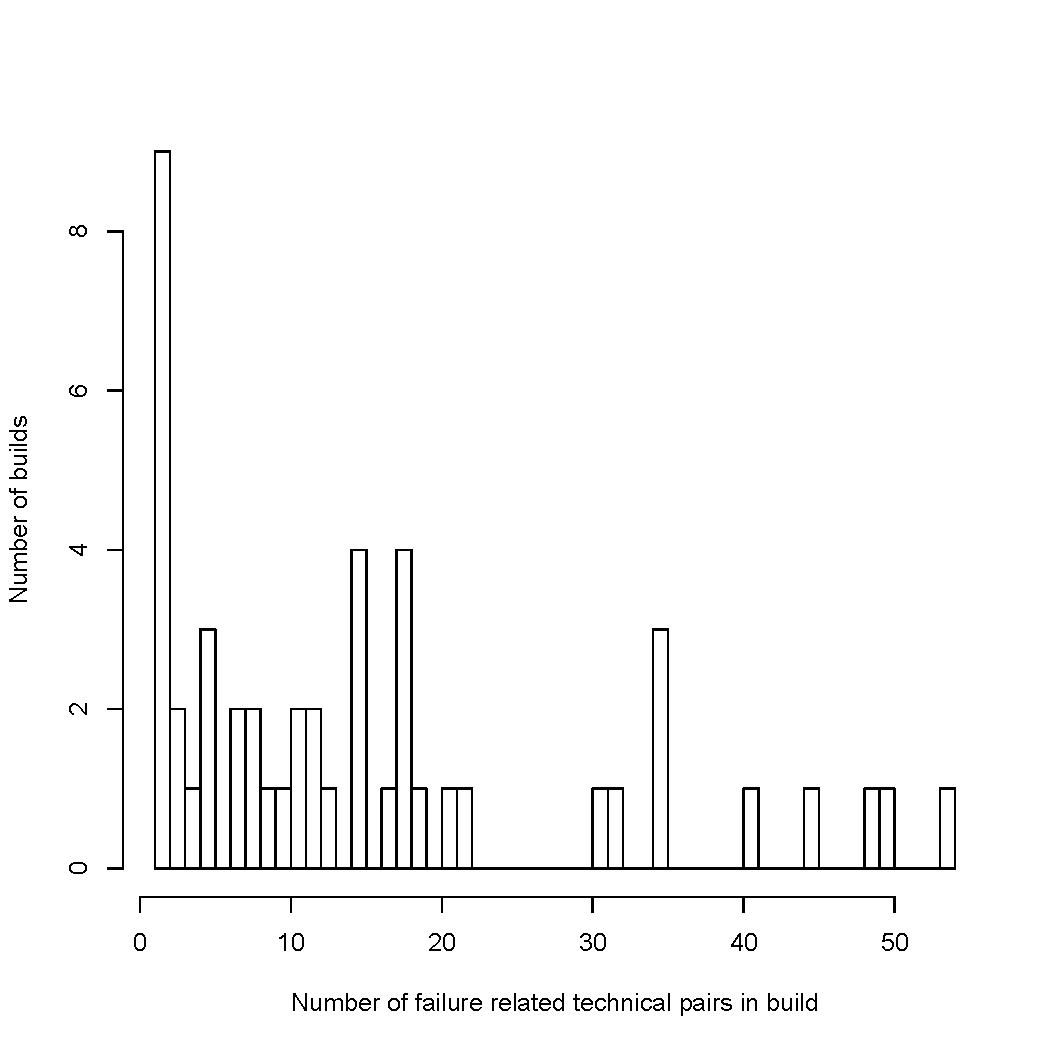
\includegraphics[width=\columnwidth]{figures/builddistribution}
\vspace{-.75cm}
\caption{Histogram plotting how many builds have a certain number of failure-reated technical pairs.}
\label{fig:builddistribution}
\end{figure}

\subsection{Discussion}
% answered the the research question
These results show that there is a strong relationship between certain technical
developer pairs and increased likelihood of a build failure.
% meaning of patterns
Out of the total of 120 technical pairs that increase the likelihood of a
build to fail, only 23 had an existing
corresponding socio-technical pair. Of these, none were statistically
related to build failure. This means that 97 pairs of developers that had a
technical dependency did not communicate with each other and
consequently increased the likelihood of a build failure. Our results not only
corroborate past findings~\cite{cataldo:cscw:2006,cataldo:esem:2008} that socio-technical gaps
have a negative effect in software development. More importantly, they indicate
that the analysis presented in this paper is able to identify the specific
socio-technical gaps, namely the actual developer pairs where the gaps occur
and that increase the likelihood of build failure. 

% contrast of t and st patterns After investigating the pairs closer with respect
% to team allocation, we found that most of the pairs span do not originate from
% the same team.
Although not a goal of this paper, we sought possible explanations for the
socio-technical gaps in this project. A preliminary analysis of developers
membership to teams shows that most
of the technical pairs related to build failure consist of developer belonging to
different teams. Naggappan et al.~\cite{nagappan:icse:2008} found that using the
organizational distance between people predicts failures. They reasoned that this
is due to the lack of awareness what people separated by organizational distance
work on. Although the Jazz team strongly emphasizes communication
regardless of team boundaries, it still seems that organizational distance has
an influence on its communication behavior.

% bridge to regression - confounding variables?
Further, although the analysis of technical pairs in relation to build failures
showed that they have a negative influence on the build result, it does not take
into account possible confounding variables. The question is if there developer pairs still effect the build outcome in the presence of confounding variables, such as number of developers involved in a build, number of work items
related to a build, number of change sets per build, and number of files changed.
We tested this using a logistical regression model including both developer pairs and confounding variables.

Overall the logistic regression confirms the effect of the developer pairs
even in the presence of confounding variables, such as number of files changed
and numbers of developers (AIC of 7006). 
Table~\ref{tab:regression} shows an excerpt from the complete logistical
regression which shows that the twenty pairs previously identified are still
significant under the influence of the four confounding variables. Because we have 2872 developer pairs, space constraints prevent us from reporting the entire regression model. We chose to report on the coefficients for the twenty pairs that we reported in Table~\ref{tab:regression} as well as the coefficients for the four control features.

All features shown in Table~\ref{tab:regression} are significant at the $\alpha=.001$ level (indicated by the p-value and ***).
We checked for all the other technical pairs that were reported significant using the approach described in the previous section and found that they are all significant in the regression model as well.
Moreover, the four control variables of number of developers per build, number
of work items per build, number of change sets per build, and number of files changed per build are also significant.

% explain the coefficient interpretation
% some of the pairs are positive
% some are negative
% extreme magnitude
Since we model failed builds with 0 and successful builds with 1, a negative coefficient means that the feature increases the chances of a failure.
All pairs reported in Table~\ref{tab:regression} and the technical pairs that we identified to be related to build failure have a negative coefficient.
 
% about the control variables
%As shown in Table~\ref{tab:regression} two of the four control features, number of change sets per build and number of developers contributing to a build increase the likelihood of a build succeeding.
%On the other hand number of files changed per build and number of work items per build increase the likelihood of a build failing.

In conclusion, we can answer our second research question with yes: there are
certain technical pairs that are significantly related to build failure, and
this happens even in the presence of possibly confounding variables. 







%\input{regression-analysis}







\section{Practical Implications}
\label{sec:implications}
Our findings have several implications for the design of collaborative systems.
By automating the analyses presented here we can incorporate the knowledge about
developer pairs that tend to be failure related in a real-time recommender
system. Not only do we provide the recommendations that matter to the upcoming
build, we also provide incentives to motivate developers to talk about their
technical dependencies. 

Such a recommender system can use project historical data to
calculate the likelihood that an upcoming build fails given a particular
developer pair that worked on that build without communicating to each other. In
the case of the pair (Adam, Bart) the system may recommend that these
developers should communicate about their technical dependencies, as there
would be a probability
of 91\% of failure of the next build should they not follow the
recommendation. This probability of failure serves as mechanism to
rank importance of a socio-technical gap and more importantly as an
incentive to act upon.

For management, such a recommender system can provide details about the
individual developers in, and properties of, these potentially problematic
developer pairs. Individual developers may be an explanation for the behavior of
the pairs we found in Jazz\texttrademark. This may indicate developers that are
harder to work with or too busy to coordinate appropriately, prompting management
to reorganize teams and workloads. This would minimize the likelihood of a build
to fail, by removing the underlying cause of a pair to be failure related.
Similarly, as another example from our study, most developer pairs
consisted of developers that were part of different teams. In such
situations management may decide to investigate reasons for coordination
problems that include factors such as geographical or functional distance in the project.




\section{Threats To Validity}
\label{sec:threats}
%\todo{rework}
During our study we identified two main threats. 
One threat covers issues that arise from the underlying data we used.
The other threat deals with possible problems from the conceptualization of
constructs in our study.

\subsection{Data}
We performed all our analysis on one set of data, the Jazz\texttrademark\
repository. This limits the generalizability of our findings, due to the fact
that we only made the observations within one project. The  
project size and the project properties -- incorporating open
source practices such as open development and encouraging community involvement
-- make us believe that our findings still hold value.

Furthermore we only investigated three months of the project's lifetime. This
might lead to smaller significance of our results. However, since the three
months are directly before a major release of the project, this dataset contains
the most viable data for our analysis. In those three months a lack of necessary
coordination is the most harmful to the project.

Another threat that is inevitable in studies of software engineers is
the possible lack of recorded communication. This and the possibility of people
coordinating without communicating, such as reading each others source
code~\cite{bolici:stc:2009}, are mitigated in Jazz by its development process.
The Jazz\texttrademark\ team's development process demands that the developers
coordinate using workitem discussion. 


\subsection{Conceptualization}
Our conceptualization of the three edges we use to construct the
socio-technical networks might introduce inaccuracy in our findings.
First, social edges are extracted from workitem discussions. We assumed that
every developer commenting on or subscribed to a work item reads all comments of that
work item. This assumption might not always be correct. By manual inspection of
a selected number of work items, however, we found that developers who
commented on a work item are aware of the other comments, confirming our assumption.

Second, the technical edges are not problematic by themselves, but they are not
complete, since there are more technical relationships between developers that
can be examined. For example, two developers can be connected if one developer
changes someone else's code. This however does not invalidate our findings, it
just suggests that there is room for improvement, which we should address
next.

Third, socio-technical edges on the other hand may suffer from the combination of
social and technical edges. For example, it is not necessarily true that the
discussion of  two developers in a technical dependency is always about their
technical dependency. 
In our study however, since the changes to
source code files we use to extract technical dependencies are attached to workitem discussion, we are
confident that they addressed the changes at least indirectly.



\section{Conclusion}
\label{sec:conclusions}
Our study investigated the relationship between pairs of developers that share
a technical dependency but do not communicate and build failures. We were
motivated by findings in the literature that suggested that high alignment between technical dependencies and actual coordination in a project has a positive effect on task
performance.
%
We hypothesized that a similar relationship may be found in relation to a broader
coordination outcome, i.e. integration outcome, because developers not
coordinating about dependencies in their work might lead to errors remaining in
the code that break the build.

Our case study of coordination in the Jazz project indicates that 
historical project information about socio-technical coordination and software
builds can be used in a model that predicts the quality of upcoming builds. We also found
that the influence of developer pairs with a socio-technical gap on the build
failure was very high. This means that if any one of these pairs was present in a
social network of a build, the build had at least an 74\% chance to fail.
Thus, we add to the literature on failure prediction with a method that
provides actionable knowledge to avoid failures. 

Besides the possible of integrating our findings into a real-time recommender system that indicates the specific developer pairs that should talk about their dependencies, our results add to the research in
collaborative software engineering. Not only do we add to the evidence about
the role of effective communication in the development of high quality
software, but our findings indicate that measures of socio-technical congruence can
serve as a mechanism to identify which inter-personal relationships are
important to avoid breaking software integrations. 
%
We plan to extend this research in a number of directions:

% \begin{description}
\emph{More specific information in socio-technical networks.}
We plan to study socio-technical coordination at a finer level by refining all
three edge types social, technical and socio-technical as well as the
information about developers. For the social edges we plan on identifying who
people are talking to and exactly about what. Technical edges can be refined by examining other source code relations, such as call
graphs, or changes made to others' source code. 
%
To combine social and technical
edges to socio-technical edges we plan to use content analysis techniques on
communication to match it to the appropriate technical edge. We also plan
on also investigating the developers that are part of the social networks more
closely by incorporating developer characteristics, such as experience,
geographical location, role or team allocation.

\emph{Additional edges that indicate emergent coordination.}
In this study we focused on technical pairs and only briefly touched on
socio-technical pairs. In the future we plan to extend this focus to include a
detailed analysis of socio-technical pairs and of those
developer pairs that communicated without sharing a technical dependency, and
which indicate emerging communication in the project, and expertize seeking
behaviors that are important to effective coordination.

\emph{Different types of failures.}
A build fails often because of a single or several failures scattered across several locations
Hence we plan on
investigating single bugs. This additionally enables us to investigate pre-release and post-relase failures separately.


%%%%%%%%%%%%%%%%%%%%%%%%%%%%%%%%%%%%%%%%%%%%%%%%%%%
%%%%%%%%%%%%%%%%%%%%%%%%%%%%%%%%%%%%%%%%%%%%%%%%%%%
%%%%%%%%%%%%%%%%%%%%%%%%%%%%%%%%%%%%%%%%%%%%%%%%%%%
%%%%%%%%%%%%%%%%%%%%%%%%%%%%%%%%%%%%%%%%%%%%%%%%%%%
%%%%%%%%%%%%%%%%%%%%%%%%%%%%%%%%%%%%%%%%%%%%%%%%%%%

\startchapter{Socio-Technical Congruence and Failure -- part II}
Coordinating the efforts of individuals working together in a team is
necessary to build software systems. The complexity of current systems require contributions
from tens or hundreds of people who may span multiple offices, cities, or even continents.
To build such systems, we need to ensure that the team is not only capable of
developing components of a system, but also has the governance to be able to integrate the
interdependent parts into a whole.

We describe a case study of socio-technical coordination and its effect on software builds in the IBM\textsuperscript{\textregistered}
Rational Team Concert\textsuperscript{\textregistered} (RTC) software product\footnote{IBM, Rational, Jazz and Rational Team Concert are trademarks or registered trademarks of International Business Machines Corporation in the United States, other countries, or both.}.
Our approach to investigating coordination is to examine the
alignment between the technical dimension of work and the social relationships
between team members. This alignment is called \textbf{socio-technical
congruence}~\cite{cataldo:cscw:2006}. High socio-technical congruence
has been shown to be a predictor of coordination success
\cite{cataldo:cscw:2006,ehrlich2008:gaps}.
The mismatches between the social and technical dimensions, or \textbf{gaps},
also have been observed as increasing resolution times for software activities.
The objective of this study is to investigate the effects of socio-technical congruence on high-coordination software development activities during a project.
%, and to examine the usefulness of the measure when drawing conclusions about collaboration around software development.

We seek to discover the relationship that congruence has on the probability that a regularly-scheduled software build will be successful.marczak:re:2008
We conduct a case study of a large software project at IBM.  A build result, which can be \emph{error} or \emph{OK}, indicates the relative health of the project up to that build. To
measure socio-technical congruence we apply two different measures: a
previously-published congruence approach \cite{cataldo:cscw:2006},
and a weighted congruence approach that provides details about the size of a
gap between two individuals~\cite{kwan2009:weighted}. We
also examine RTC's processes and tools to identify any
explanations of the relationship between congruence and builds that
we find.

Our results indicate that congruence affects build success probabilities for certain types of builds.
In a continuous build, which may involve changes submitted primarily by a co-located team, high congruence leads to a higher probability of build success.
However, in an integration build, which involves code submitted by many distributed teams, high congruence actually reduces the probability of build success.
Although the congruence per build is relatively low at approximately 20\% overall, the team is able to coordinate to complete their builds.
We also find that the mean size of a congruence gap correlates inversely with build success probability.
Our findings on the socio-technical congruence and build quality in RTC are complemented by insights we
obtained by studying the context of the RTC project. Some of these results may be explained also by the congruence conceptualizations that we use in our empirical study.
% By using the weighted congruence measure we could investigate gaps in coordination at a fine level of detail and unveil interesting patterns in the teams' coordination behaviour.

Our case study adds to the scarce but needed empirical evidence about
socio-technical congruence measures in the investigation of coordination in
software projects, and allows us to
discuss improvements to congruence conceptualizations and measures. 

The paper begins with background on the need for coordination in software
projects and socio-technical congruence, and motivates the applicability of
socio-technical congruence to our case study setting in Section
\ref{sec:background}. We discuss related
work in Section \ref{sec:relwork} and describe the research objective in Section \ref{sec:objective}. We then describe
in Section \ref{sec:congruence} the two measurements for socio-technical
congruence that we used in our case study: an unweighted congruence measurement
found in the literature \cite{cataldo:cscw:2006}, and a weighted congruence measurement from
our own work \cite{kwan2009:weighted}. We describe our research questions and
methodology in Section \ref{sec:methodology}, and outline
the results in Section \ref{sec:results}. Our discussion 
in Section \ref{sec:discussion} provides an explanation of the effects we
observed. We conclude the paper by
outlining the threats to validity in our study in Section
\ref{sec:threats} and conclude in Section \ref{sec:conclusion}.

%--------------------------------------------------------------------------------------------------------------
\section{Background and Motivation}
\label{sec:background}

% The level of complexity in a software project far exceeds the complexity in many other disciplines. One reason for this complexity is the large number of interdependencies between software components. In addition, the introduction of other artifacts, including contracts, project plans, requirements documents and rationales, test documents, and end-user documentation introduces further dependencies.

%An organization must have the capacity to monitor and support its people as they execute their development tasks.

%Developers who work on related software components should coordinate their efforts with each other. 
%However, as it is difficult to measure coordination quality, one approach, called socio-technical congruence~\cite{cataldo:cscw:2006} has been proposed as a ``fine-grained measure of coordination''.

%Why do we need coordination in software projects? How can we study the relationship between coordination and software quality?
Here we discuss coordination in software engineering and discuss socio-technical congruence as a way to measure coordination quality. We then present our case study of the IBM Rational Team Concert\textsuperscript{\textregistered} project.


%------------------------------------------------------------------------- 
\subsection{The Need for Coordination}

Software is extremely complex because of the sheer number of dependencies~\cite{sawyer2004:teams}.
Large software projects have a large number of components that interoperate with one another.
The difficulty arises when changes must be made to the software, because a change in one component of the software often requires changes in dependent components~\cite{desouza:2008}. Because a single person's knowledge of a system is specialized as well as limited, that person often is unable to make the appropriate modifications in dependent components when a component is changed.

Coordination is defined as ``integrating or linking together different parts of an organization to accomplish a collective set of tasks''~\cite{vandeven1976}. In order to manage changes and maintain quality, developers must coordinate, and in software development, coordination is largely achieved by communicating with people who depend on the work that you do \cite{kraut:1995coordination}.

A successful software build can be viewed as the outcome of good coordination because the build requires the correct compilation of multiple, dependent files of source code.
A failed build, on the other hand, demotivates software developers \cite{holck2004,damian:icgse:2007} and destabilizes the product \cite{cusumano1997}.
While a failed build is not necessarily a disaster, it slows down work significantly while developers scramble to repair the issues.
A build result thus serves as an indicator of the health of the software project up until that point in time.
%If the developers successfully coordinate the integration of code between the previous build and the upcoming build, then the build should succeed.

Thus, a developer should coordinate closely with individuals whose technical dependencies affect his work in order to effectively build software. This brings forth the idea of aligning the technical structure and the social interactions \cite{herbsleb2007:fose}, leading us to the foundation of socio-technical congruence.

%-------------------------------------------------------------------------
\subsection{Socio-technical Congruence}

Socio-technical congruence is defined as the match between the coordination needs established by the technical domain and the actual coordination activities carried out by project members. Socio-technical congruence in software engineering was brought to attention by Cataldo, et al.~\cite{cataldo:cscw:2006}, though the concept has been explored in engineering \cite{browning2001} and management science \cite{henderson1990}. A \textbf{coordination need} indicates that two persons should be coordinating based on the technical dependencies on the project. A coordination need is determined by analysing the assignments of people to a technical entity such as a source code module, and the technical dependencies among the technical entities.
Socio-technical congruence states that if there is a coordination need between two people, these people should be coordinating.
For example, if two people work on different, but dependent components of the project, then those persons should be coordinating with each other.

If two individuals have a coordination need, but do not coordinate, then there is a \textbf{gap} between these two individuals. A gap suggests the existence of a coordination problem. One of the goals of socio-technical congruence is to minimize the number of gaps, either by maintaining good coordination between individuals who have a coordination need, or by reducing the number of technical dependencies in the project and therefore reducing the coordination needs~\cite{sarma2008:measuring_stc}.

What socio-technical congruence offers is an approach to measure the coordination quality~\cite{cataldo:cscw:2006}. We can use this measurement to identify the effect of socio-technical coordination on software build quality.


%We study RTC because it is a large project that has high coordination needs. RTC involves 151 active contributors working in 47 different teams spread across 7 geographical locations. The team builds their software nightly, weekly, and during integration periods prior to release. Such a large team spread across long distances certainly encounters coordination challenges. The team also records written conversations that take place around work items, which are enhancements, defects, or tasks related to the project.

%Because of the heavy technical dependencies among components as well as the recorded conversation, RTC becomes an interesting case in which we can investigate socio-technical congruence and its effects on build quality.

%\subsection{Project: RTC}

\subsection{IBM Rational Team Concert Case Study}

%In our research we conducted a study on RTC by IBM.
%We choose this project because it is a project with high coordination needs and a large amount of recorded communication.
IBM Rational Team Concert, or \textbf{RTC}, is a collaborative software development tool built on the Jazz\textsuperscript{\texttrademark} architecture. It incorporates the integrated development environment, the source-code control system, the issue-tracking system, and collaborative development tools. The RTC team self-hosts, meaning that the team uses its own software to develop subsequent versions.

The following qualities make RTC an attractive case in which to study
socio-technical coordination: (1) the distributed team, (2) the iterative
process, and (3) the rich data repository. Because distribution makes coordinating work difficult~\cite{hinds:cscw:2006,herbsleb2003:speed}, RTC is supposed to enhance communication among project members by providing collaborative facilities~\cite{frost:ieeesoftware:2007}. Developers explicitly record communication across sites using the product.
RTC's iterative process encourages developers to ``build early and often''. In addition to supporting continuous builds, RTC does frequent integration builds, providing a large amount of data to analyse.
% The encouraged community involvement and the openness to the community poses extra stress on the developers because of the increased information input they get~\cite{fussell98:overload}.

At the time of our study, the RTC development team involved a team distributed over 16
different sites located in the United States, Canada, and Europe. Seven sites were
active in RTC development and testing. There were 151 active contributors
at these locations. Each team, which was not necessarily confined to one geographical location,
was responsible for developing a component of RTC.
The team sizes ranged from 1 to 20 and had an average of 5.7 members. The number
of developers per geographical site ranged from 7 to 24 and was 14.8 on average.

The project uses the \emph{Eclipse Way} development process~\cite{frost:ieeesoftware:2007}.
It defines six-week iteration cycles, which are separated into planning,
development and stabilization activities. A project management committee
formulates the goals and features for each release at the beginning of the each
iteration, and \emph{work item}s represent assignable and traceable tasks for each
team. RTC's process encourages frequent building, including continuous, nightly, weekly, and integration builds.

%The RTC team is self-hosting, meaning that it uses the software system that it develops. Of particular note is the team's use of Rational Team Concert, which is a client-sidedevelopment environment that integrates programming, source code control, report generation and delivery, issue-tracking, and project planning into one system.

One unique aspect of RTC is its ``open-commercial'' development model. RTC is a commercial product developed by IBM, but has a publicly-accessible issue-tracking and reports system. This open-commercial model allows a large amount of information to flow into the team from the community.
Communication between individuals is done through the issue-tracking comments, through instant messaging, through Internet Relay Chat, by phone, and face-to-face. Personal email is discouraged. The team uses a mailing list to deliver announcements, such as server maintenance schedules. 
%The team recommends that discussions that do not occur in public channels are summarized as work item comments so that remote team members are able to track decisions and rationales.


\section{Related Work}
\label{sec:relwork}

Socio-technical congruence was proposed initially as a fine-grained measure of coordination that can be used to diagnose coordination problems in a software development team~\cite{cataldo:cscw:2006}.
The original conceptualization of socio-technical congruence was in Conway's Law, which observed that
product architecture reflects organizational structure~\cite{conway:datamination:1968}.

Socio-technical congruence has been recognized as an important element of product
design in the management sciences field~\cite{sosa2004:manage}. The socio-technical congruence community goes one step further
and declares that not only does this alignment happen as a consequence of product
architecture, but that it is in fact desired
\cite{sarma2008:measuring_stc,valetto2007:value}. Unfortunately there are only a
handful of empirical research results that discuss the effects of the
socio-technical congruence approach on software teams.

% First, we review research on studies of coordination in software engineering, and then we review related work on socio-technical congruence.

\subsection{Coordination in Software Teams}

%There has been a recent resurgence of interest in the collaborative aspects of software engineering.

Research in software-engineering coordination has examined interactions among
software developers \cite{carter2004,marczak:re:2008}, how they acquire
knowledge \cite{ehrlich:icgse:2006,nakakoji2010:rdc}, and
how they cope with issues including geographical
separation~\cite{espinosa2007:team_knowledge,herbsleb2003:speed}.
The ability to coordinate has
been shown as an influential factor in customer satisfaction \cite{kraut:1995coordination} and  improves the capability to produce quality work~\cite{faraj2000}.

%Redmiles and de Souza studied two software teams, especially with respect to their awareness mechanisms, and found especially that a modular software architecture makes a developer's awareness network more manageable~\cite{desouza2007:awarenessnetwork}.

%The studies have also shown relationships between communicating and build quality. Communication patterns have also been used to predict build quality, suggesting that even the network structures have an influence on build outcomes \cite{wolf:icse:2009}.

% ,herbsleb1995:ooad
Software developers spend much of their time
communicating~\cite{perry94}. Because developers face
problems when integrating different components from heterogeneous environments,
%~\cite{redmiles2007:continuous}
developers engage in direct or indirect
communication, either to coordinate their activities, or to acquire knowledge of
a particular aspect of the software ~\cite{nakakoji2010:rdc}.
Herbsleb, et al. examined the influence of coordination on integrating software
modules through interviews~\cite{herbsleb1999:architectures}, and found that
processes, as well as the willingness to communicate directly, helped teams
integrate software. De Souza, et al.~\cite{desouza2007:awarenessnetwork} found that implicit
communication is important to avoid collaboration breakdowns and delays. Ko, et al.~\cite{ko:icse:2007} found that developers were identified as the main source of knowledge about code issues.
Wolf, et al.~~\cite{wolf:icse:2009} used properties of social networks to predict the outcome of integrating the software parts within teams.
This prior work establishes the fact that developers communicate heavily about technical matters.

%Both types of coordination are essential to avoid problems during software development~\cite{} ANDRESMISSINGPAPER

Coordinating software teams becomes more difficult as the distance between people increases \cite{herbsleb:icse:2001}.
Studies of Microsoft~\cite{bird2009:dds_quality,nagappan:icse:2008}
show that distance between people that work together on a
program determine the program's failure proneness.
Differences in time zones can affect the number of defects in software projects \cite{cataldo2009:quality}.

Although distance has been identified as a challenge, advances in collaborative
development environments are enabling people to overcome challenges of distance.
One study of early RTC development
shows that the task completion time is not as strongly affected by distance as in previous studies~\cite{Nguyen:2008Distance}. Technology that empowers distributed collaboration include topic recommendations~\cite{carter2004} and instant messaging~\cite{niinimaki2008}. Processes are adapting to the fast pace of software development: the Eclipse way~\cite{frost:ieeesoftware:2007} emphasizes placing milestones at fixed intervals and community involvement.
% However, the frequent communication that technology enables has also caused problems~\cite{desouza2007:awarenessnetwork,damian:icgse:2007}.

%Researchers have conceptualized coordination in many different ways, including
%direct communication, indirect communication, proximity, and
%awareness~\cite{ehrlich:icgse:2006,espinosa2007:team_knowledge,cataldo:cscw:2006,damian2010:rdc}.
%Socio-technical congruence allows us to determine if an organization has good coordination practices.
%


\subsection{Effects of Socio-technical Congruence}



Current research suggests that attaining a high level of socio-technical congruence is beneficial to an organization.
Evidence shows that higher congruence leads to faster completion of modification requests~\cite{cataldo:cscw:2006}. 
The presence of gaps increases the number of code changes \cite{ehrlich2008:gaps}, and a lack of coordination connections across system and organizational boundaries have a negative effect on performance~\cite{sosa2004:manage}.

Socio-technical gaps have been found to be an issue not only because they lower
the congruence and thus lower productivity~\cite{cataldo:cscw:2006}, but because they are especially problematic in the context of distributed development~\cite{ehrlich2008:gaps}. Thus, researchers have proposed remedial actions when socio-technical congruence gaps are discovered~\cite{valetto2007:value}. 
Examples of actions include closing a gap by augmenting coordination and eliminating the gap by refactoring software.

% ~\cite{curtis1988}
The usefulness of socio-technical congruence depends on the conceptualizations of
the social and the technical dimensions. Communication is believed to help people coordinate. However, it is not the only way to describe the social dimension. 
For instance, Cataldo et al.~\cite{cataldo:cscw:2006} evaluated congruence in the context of software development using different representations of actual coordination, including geographical proximity, IRC communication, and issue-tracking comments; these factors correlate with the resolution time of modification requests. There are also variations in the way technical dependencies can be handled. Cataldo et al.~\cite{cataldo:esem:2008} used differing ways to measure architectural dependencies and found that the congruence values computed using a ``files changed together'' dependency are more reliable than call graph dependencies~\cite{deSouza2004:thwarts_collaboration}. Gokpinar, et al \cite{gokpinar2010} applied a congruence technique and discovered that a higher coordination deficit leads to a larger number of filed incident reports, implying reduced quality.

Socio-technical congruence has been explored outside of the software development field, particularly in engineering and management disciplines \cite{henderson1990,sosa2004:manage,gokpinar2010,sosa2008}. Sosa \cite{sosa2008} described a formal technique to compute socio-technical congruence and identified ``potentially unattended technical interactions'', which are technical dependencies in modules that are not monitored. Gokpinar \cite{gokpinar2010}, independently of our work, developed a weighted socio-technical congruence technique that he applies to the automotive industry.

In summary, there is a need to coordinate effectively in software development across technical dependencies that may cross geographical boundaries, and socio-technical congruence is a useful mechanism for studying coordination.
%, and (3) that there is a need to coordinate across technical dependencies.


% The rationale is that, because a successful software build requires aligned module dependencies, and because high socio-technical congruence leads to improvements in the alignment of these dependencies, high socio-technical congruence should improve the chance of a successful software build.


\section{Research Objective}
\label{sec:objective}

Our research objective in this paper is to study the applicability of socio-technical congruence on a large, distributed software team. The theory of socio-technical congruence suggests that increasing socio-technical congruence will improve the outcome of a software development activity that requires a high amount of coordination.

We use a software build as our coordination-intensive software development activity and unit of success. A build result is ``OK'' when the software compiles with no errors and passes every test case. A build result is ``error'' when an error is discovered during compiling or testing. We know that builds are important to the RTC team: to them, build quality is almost synonymous with code quality. An OK build implies that the team was able to achieve a successful outcome, and an error build implies that the team had a problem during development.

We conceptualize a coordination need between two individuals as a relationship indicating that these two individuals change the same file before a build. We conceptualize actual coordination between two individuals as an instance in which each individual writes at least one comment in at least one work item associated with either of the file changes. The size of a gap between two individuals indicates the proportion of actual coordination over the coordination needs. A small gap size suggests that there is a sufficient actual coordination to cover the coordination needs.

We hypothesize that, when using congruence calculated by ``files changed together'' and ``work item co-commenting'', increasing congruence results in an increase in the probability of a successful build result. We also anticipate that a decrease in gap size increases the probability of a successful build.

Due to our conceptualizations, we expect that our calculated congruence values may be lower than what occurs in reality. First, our conceptualization will likely underestimate the actual coordination occurring in the project.
% The RTC team uses the commenting system frequently, but our conceptualization cannot take into account direct, point-to-point communication between developers on a particular topic.
Second, our dependencies may overestimate the dependencies between files in RTC.
As RTC is a distributed project that follows a modular design, it is possible that many changes are not as strongly dependent as our conceptualization suggests. Nonetheless, in absence of more detailed data we believe that our conceptualizations capture the relationships between developers and illustrate potential dependencies where coordination issues may occur and contribute to a build failure.

We use two different congruence measurements to explore what advantages a new measure can provide. The first congruence measurement is an unweighted technique developed by Cataldo, et al.~\cite{cataldo:cscw:2006}. The second congruence measurement is a weighted technique from our previous work~\cite{kwan2009:weighted}, which offers additional features such as relationship strength between two people and variable size of a socio-technical congruence gap.

\subsubsection*{Research Question 1: Does socio-technical congruence have an effect on build success probability in RTC?}

\vspace{6pt}

\subsubsection*{Research Question 2: Does gap size have an effect on build success probability in RTC?}

\vspace{6pt}

Our work differs from previous socio-technical congruence studies because it applies two different congruence measures on software builds that occur every one to six weeks in a single project. This differs from previous studies that apply congruence to entire project releases. To our knowledge no application of weighted congruence has been applied to software engineering.

% In the next section (Section \ref{sec:congruence}), we present two approaches to calculate congruence: an unweighted
% congruence measurement developed by Cataldo et al.~\cite{cataldo:cscw:2006}, and a weighted
% congruence measurement from our own work~\cite{kwan2009:weighted}. Gap size is defined in Section \ref{sec:lack}.

% We then present our research methodology, followed by our study results.


\section{Calculating Congruence}
\label{sec:congruence}

We describe unweighted congruence as presented by Cataldo et al. \cite{cataldo:cscw:2006} in Section \ref{sec:stc}. Weighted congruence~\cite{kwan2009:weighted}, described in Section \ref{sec:measure} is a weighted congruence measure from our work that addresses limitations of unweighted congruence.

\subsection{Technical Entities and Social Relationships}

A \textbf{technical entity} is an entity in a project that can be worked on by a person. Examples of a technical entity include a source code file, a compiled binary, a requirement, a task, or a bug. Socio-technical congruence has focused on the source code file as the technical entity \cite{cataldo:cscw:2006, ehrlich2008:gaps}, although work has also examined socio-technical congruence using a requirement~\cite{damian2010:rdc,marczak2009:crossfunctional} or a task~\cite{wolf2009:mining} as the technical entity. The choice of technical entity depends on the context of the study.
% A person is assigned to work on one or more technical entities.

At the core of socio-technical congruence is the concept of a technical dependency. A \textbf{technical dependency} is a type of dependency between two technical entities. Examples of technical dependencies are in Box \ref{ph:technicalunits}.

% \begin{float*}
\begin{placeholder}[t]
\begin{itemize}
\item Requirements that depend on each other~\cite{marczak:re:2008,marczak2009:crossfunctional}
\item Source code modules changed together in a change set~\cite{cataldo:cscw:2006,cataldo:esem:2008}
\item Source code that has a call-graph dependency~\cite{deSouza2004:thwarts_collaboration}
\item Tasks that depend on other tasks \cite{wolf2009:mining}
\end{itemize}

\caption{Examples of technical dependencies}
\label{ph:technicalunits}
\end{placeholder}


% \end{float*}

A \textbf{coordination need} is a relationship that indicates that two people should be coordinating, based on the assignment of each person to a technical entity, and the technical dependencies between the entities.

Social relationships are identified through \textbf{actual coordination}, which indicates how people in the organization are actually coordinating. Note that, despite the nomenclature ``coordination'' used in previous work \cite{cataldo:cscw:2006}, the actual coordination matrix does not need to represent coordination at all, but merely a relationship of interest between two people in an organization. Generally, one would want to choose relationships that are of interest to the performance of the organization, hence favouring the selection of relationships such as ``communication''. Examples of actual coordination appear in Box \ref{ph:relationships}.
%Actual coordination may also be represented as a composite of relationships~\cite{ehrlich2008:congruence_gaps}.




\subsection{Calculating Socio-Technical Congruence}
\label{sec:stc}

Given $m$ people, and $n$ technical entities to examine, the coordination needs are calculated as 

\[ CN = A \times D \times (A)^t \]

\noindent where $A$ is an $m \times n$ assignment matrix that indicates that a person is assigned to a technical entity of the project, and $D$ is a $n \times n$ technical dependency matrix that indicates that a technical entity is dependent on another technical entity~\cite{cataldo:cscw:2006}. The result is $CN$, an $m \times m$ coordination needs matrix that indicates who in the project should be coordinating with whom.

% In the technical dependency matrix, a technical entity is dependent on itself. The reason this assumption is made is best illustrated with an example. Person A and Person B are both assigned to work on the same technical entity. If we do not assume a technical entity is dependent on itself, then in the coordination needs matrix, Person A and Person B do not have a coordination need with each other even though they work on the entity.

Once the coordination needs matrix is calculated, congruence is calculated by comparing this matrix to an actual coordination matrix. If an edge exists in the actual coordination matrix, and the same edge exists in the coordination needs matrix, then there is congruence on this edge. Given definitions

% \[ congruence = \frac{\displaystyle\sum^{m}_{i=1} \sum^{m}_{j=1} CN_{ij} - \sum^{m}_{i=1}\sum^{m}_{j=1}AC_{ij}}{\displaystyle\sum^{m}_{i=1}\sum^{m}_{j=1}CN_{ij}} \]

\[ \text{Diff}(CN, AC) = card\{ \text{diff}_{ij} | CN_{ij} > 0 \& AC_{ij} > 0 \} \]
\[|CN| = card \{ CN_{ij} > 0 \} \]

\noindent the socio-technical congruence index is calculated as~\cite{cataldo:esem:2008}

\[ \text{congruence} = \frac{\text{Diff}(CN, AC)}  {|CN|} \]

\noindent where $AC$ is an $m \times m$ matrix representing actual coordination. The resulting congruence value is a number between 0 and 1, where 0 indicates no congruence, and 1 indicates full congruence.
% If there are people involved in the actual coordination matrix that do not appear in the assignment matrix, these additional people are ignored.

% In the case when there are no coordination needs, socio-technical congruence is undefined. If there are no technical dependencies or no coordination needs between different individuals, then presumably the work can be accomplished by a single person.

\begin{placeholder}[t]
\begin{itemize}
\item Communication---A communicates with B~\cite{cataldo:cscw:2006, ehrlich2008:gaps, cataldo:esem:2008,damian2007:collaboration}.
\item Location---A is in the same location as B~\cite{cataldo:cscw:2006, ehrlich2008:gaps}.
\item Team structure---A is in the same team as B~\cite{cataldo:cscw:2006}.
\end{itemize}
\caption{Examples of actual coordination}
\label{ph:relationships}
\end{placeholder}

\subsection{Limitations of the Unweighted Socio-technical Congruence Calculation}
 
Unfortunately, the unweighted congruence measure has a limitation because socio-technical congruence identifies if a coordination need is either satisfied, or not satisfied, with no values indicating relative strengths.

The missing strengths prevent the identification of gaps that may be large or high-priority gaps that require attention.  Previous research has shown that projects succeed despite the presence of gaps. Marczak, et al.~\cite{marczak:re:2008} identified a project that delivered requirements on time despite the existence of gaps. 
Ehrlich, et al.~\cite{ehrlich2008:gaps} suggest that having an individual act as an intermediary between two groups, known as a \emph{broker}, may be able to mitigate the effect of gaps.
Communication structures may compensate for a lack of congruence~\cite{hinds:cscw:2006}. Literature in areas such as management science supports the idea that gaps are not a liability, but simply a reality~\cite{deSouza2004:thwarts_collaboration,hossain:cscw:2006}.

As developers have multiple dependencies~\cite{desouza2007:awarenessnetwork,mockus2002:opensource}, one would presume that those pairs with more coordination needs would need to coordinate more. Current socio-technical congruence provides no way to identify which pairs have high coordination needs. Researchers have suggested that both social and technical dependencies should be weighted \cite{valetto:msr:2007,kwan2009:weighted}, 
%They suggest that the number of changes made to the same artifact, or the number of dependencies of a source file onto another are possible candidates for weights,
but do not evaluate their proposed changes.

%Thus, we believe that one of our objectives is not to eliminate every gap, but rather to identify which gaps in a matrix have high coordination needs and which gaps are not satisfied by actual coordination. 

% In the next section, we propose a new method to calculate socio-technical congruence to address this limitation.



%Unfortunately, the measure of congruence presented by Cataldo, et al~\cite{cataldo:cscw:2006} bears some limitations. One limitation is that it uses dichotomized values for its relationships between people, resulting in a coarse interaction model.

%% A congruence ``gap'' is an instance in a social matrix where a coordination need is suggested between two specific individuals, but no actual coordination exists between these individuals. The meaning of a gap in socio-technical congruence is still not fully understood. Previous work by Ehrlich, et al. \cite{ehrlich2008:congruence_gaps} explored the implications of having gaps in a matrix and discovered that gaps appear to have a negative effect on developer performance; in this case, performance is conceptualized by the size of a change.

%Literature in other areas, namely social network analysis and management science supports the idea that gaps are not necessarily a liability, but simply a reality \cite{deSouza2004:thwarts_collaboration,hossain:cscw:2006,burt2004}. 

%Thus, we believe that one of our objectives of a method for congruence is not to minimize gaps, but rather to qualify which gaps in a matrix have a detrimental effect on project performance in order to calculate a more accurate congruence measurement. In addition, if we know to what degree a gap impedes project performance, then we can identify and prioritize congruence gaps that should be repaired.

\subsection{A Weighted Congruence Measurement}
\label{sec:measure}

We present an extension to congruence based on prior work~\cite{kwan2009:weighted} that addresses the
limitation discussed in the previous section. The intention is that this improvement will
provide more information about coordination behaviour than the current congruence measure. 

\subsubsection{Weighted Coordination Needs}
\label{subsec:ourmeasure}

\begin{figure*}
  \centering
  \subfloat[The coordination needs]{
    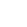
\includegraphics[width=20px]{figures/whitespace}
	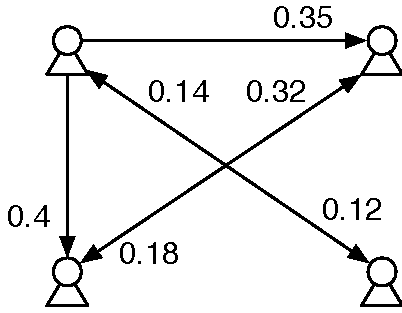
\includegraphics[width=0.38\columnwidth]{figures/coordRequirement}
	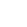
\includegraphics[width=20px]{figures/whitespace}
     \label{subfig:coordRequ}
  }
  \hspace{12pt}
  \subfloat[The actual coordination]{
    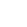
\includegraphics[width=20px]{figures/whitespace}
    \includegraphics[width=0.38\columnwidth]{figures/actualCoord}
    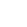
\includegraphics[width=20px]{figures/whitespace}
    \label{subfig:actualCoord}
  }
  \hspace{12pt}
  \subfloat[The coordination that is lacking]{
    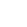
\includegraphics[width=20px]{figures/whitespace}
    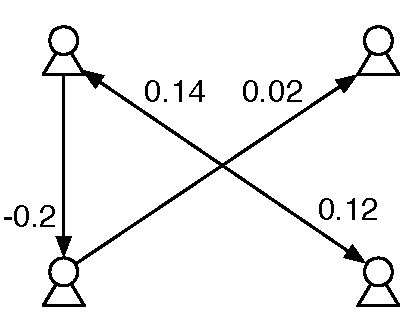
\includegraphics[width=0.38\columnwidth]{figures/coordLack}
    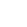
\includegraphics[width=20px]{figures/whitespace}
    \label{subfig:coordLack}
  }
	\caption{Comparing coordination needs with actual coordination to find lacking coordination}
	\label{fig:communication}
\end{figure*}

This measurement assigns a number between 0 and 1 to each entry in the task assignment, task-dependency, and actual coordination matrices.
The weighted assignment matrix is a $m\times n$ matrix where $m$ is the number of people and $n$ denotes the number of entities. 
Each entry in the matrix illustrates the strength of the connection between a person $i$ and an entity $j$. Such a connection may be the expertise person $i$ has with a task $j$, or the priority that person $i$ places on task $j$.

The weighted dependency matrix is an $n\times n$ matrix where $n$ denotes the number of entities.
Each entry in the matrix describes the strength of the relationship between two entities. The weighted dependency matrix may show the ratio of dependencies an entity has with another over the number of total dependencies that entity has on others. 
For example, an entity strongly coupled with another has a high entity dependency.

To calculate the coordination needs matrix, we use the same formula proposed by Cataldo, et al.~\cite{cataldo:cscw:2006}, using the weighted values in the task assignment $A'$ and task dependency $D'$ matrices.

\[ CN' = A' \times D' \times (A')^t \]

\noindent This calculation will yield the weighted coordination needs matrix $CN'$, an $m\times m$ people by people matrix (Figure \ref{subfig:coordRequ}).
The coordination needs matrix shows how strong the relations between people are supposed to be based on their technical work.

\subsubsection{Weighted Actual Coordination}

Weighted actual coordination is a relative value that indicates the strength of a relationship between two individuals (Figure \ref{subfig:actualCoord}). A social network such as a communication network can be weighed according to the amount of ongoing communication. For example, one such weighing scheme may work as follows:

\begin{enumerate}
\item For a communication network, identify the largest value of communication between two individuals.
\item Divide all other values by the largest, thus normalizing the communication.
\item The result is a number between 0 and 1, where 1 indicates the largest value of communication in the network, and 0 is no communication.
\end{enumerate}

Other relationships that may be used as actual coordination are the amount of distance between individuals and how frequently they meet with other members in their team.

%\begin{comment}
%\subsection{Schemes for Weighing Actual Coordination}

%\begin{placeholder}
%\begin{itemize}
%\item Person--Artifact: Degree of assignment. The number of hours, proportionally, that someone is assigned to a task.
%\item Person--Artifact: The expertise a person has about a task, based on a known metric, such as the number of contributions made to a particular component of the software.
%\end{itemize}
%\label{box:weighted_congruence_schemes}
%\caption{Example Schemes for Weighted Congruence}
%\end{placeholder}

%Different actual coordination measurements may be used for the congruence calculation. We present a few examples of techniques that can be used to weigh actual coordination matrices:

%\textbf{Communication} A social network such as a communication network can be weighed according to the amount of ongoing communication. Consider Alice and Bob that work on dependent tasks:

%\begin{enumerate}
%	\item If Adam talks to Bart about his interdependent tasks, then for each task discussed the weight is increased by $a\cdot1/n$, where $a$ is the weight of the communication and $n$ is the number of Adam's tasks that depend on Bob's tasks.
%	\item In case Adam discusses a task dependency very frequently with Bart, then, given a three point scale ``occasionally/frequently/very frequently'', $a$ is set to 1. For another task that is only occasionally discussed, $a$ would be $0.\bar{3}$.
%\end{enumerate}
%In the end, if only two of Adam's tasks depend on Bart's tasks, the weight of Adam actual coordinating with Bart would be $1.0\cdot1/2+ 0.\bar{3}\cdot1/2= 0.6\bar{6}$.

%Another scheme is to scale the amount of communication to a value relative to the maximum number of comments in the network.
%\begin{enumerate}
%\item For a communication network, identify the largest value of communication between two individuals.
%\item Divide all other values by the largest one.
%\item The result is a number between 0 and 1, where 1 indicates the largest value of communication in the network, and 0 is no communication.
%\end{enumerate}

%\textbf{Distance}
%We can also measure the relationship between Alice and Bob by looking at different types of distance.
%We can measure:
%\begin{itemize}
%\item how far they are apart in terms of physical distance, like meters or kilometres,
%\item the time difference between their time zones, and
%\item the number of organizational units that part them.
%\end{itemize}
%These values are normalized to fit within 0 and 1. All three of those measures result in a symmetric matrix, meaning Alice will always have the same distance to Bart and vice versa.
%	
%After we weigh all entries within the task assignment, task dependency, and actual coordination matrix, we can compare the coordination requirements with the actual coordination using the method described in Section \ref{subsec:ourmeasure}.
%%We discuss next the expected benefits from this weighted approach.
%\end{comment}


%------------------------------------------------------------------------- 
\subsection{Identifying Gaps in Socio-Technical Congruence}
\label{sec:lack}

%Currently, there is no formal technique to identify which pairs of individuals have a gap in congruence.
We complement our
weighted congruence measure with a technique to generate a \emph{lack-of-coordination matrix}. This matrix not only identifies the
gaps between a coordination needs matrix and an actual coordination matrix, but can also identify the size of these gaps (Figure \ref{subfig:coordLack}). This lack-of-coordination matrix can be used with both unweighted congruence and weighted congruence.

% \[ g_{ij}(CN'_{ij}, AC'_{ij}) = \Big\lbrace \begin{array}{ l l } 1 \text{,}  & CN'_{ij} - AC'_{ij} > 0 \\ 0 \text{,} & \text{otherwise} \end{array} \]
 \[ g_{ij}(CN'_{ij}, AC'_{ij}) = CN'_{ij} - AC'_{ij} \]

\noindent for $i=1,\dots,m$ and $j=1,\dots,m$. The value of $g_{ij}$ is the \textbf{gap size} between the pair $ij$. The lack-of-coordination matrix illustrates situations where the proportion of communication exceeds the expected proportion of coordination needs. If the value is positive, then there is not enough coordination to satisfy the information needs requested by the $CN'$ matrix, resulting in a \textbf{gap}. If a value is negative, then there was more coordination than requested through the $CN'$ matrix, resulting in \textbf{overload}.  Neither situation necessarily results in a problem, but we believe that investigating overload and lack of coordination has implications on software engineering coordination.

% The values in this matrix may be normalized to create a relative distance between the coordination needs and communication. 

\subsection{Weighted Congruence Index}


To convert the lack-of-coordination matrix to a single socio-technical congruence measurement, we apply

\[ \text{congruence} = 1 - \frac{\displaystyle\sum^{m}_{i=1} \sum^{m}_{j=1} g_{ij}}{\displaystyle\sum^{m}_{i=1}\sum^{m}_{j=1}CN'_{ij}} \]
\noindent for each $i$ and each $j$, unless $i=j$. This value, which is usually between 0 and 1, is an overall level of the congruence in the current network. In theory, the formula allows the index to fall outside of this range for some edge cases, but we did not observe any such cases in practice.


\subsection{Benefits of Weighted Congruence}
\label{sec:benefit}

Using a weighted congruence model allows us to deal with situations that are not handled with unweighted congruence.
% We can investigate relationships between people and the technical entities in finer-grained detail, including situations where people have multiple coordination needs with others. 
Using the weighted congruence approach allows a person diagnosing the organization to benefit from \emph{locality} and \emph{relationship strength}.

\textbf{Locality}
allows us to identify which area of a network has a gap.
% Not only does this give us an overall measure of congruence, but now we can identify potential coordination problems in the network.
The lack-of-coordination matrix identifies which pairs of individuals do not fulfill coordination needs.
Although the original model does give us some limited locality in the sense of identifying congruence gaps, it is far more coarse grained.


%Using weighted congruence, we can identify people working on two interdependent tasks who do not discuss both technical entities.

\textbf{Relationship strength}
indicates how strong the relationship between two developers is. Relationship strength allows us to identify pairs of people who have multiple coordination needs, and therefore who need to coordinate more often with each other. Using relationship strength allows us to investigate coordination in more detail because we can investigate pairs with strong dependencies---these people also tend to be key individuals in a team.
\\

%ranks people pairs where more coordination might be needed by the computed lack of congruence.
%Ranking is a considerable improvement over Cataldo's model since it allows us to only extract an unordered list of gaps. 
%This also covers gaps, but does not necessarily priorates gaps more.
%Because filling congruence gaps can be risky~\cite{valetto2007:value,ehrlich2008:congruence_gaps}, a ranking can provides us with a better assessment of which gaps to fill first if at all.


\indent By allowing better locality and relationship strength, we believe that this weighted model provides an in-depth technique with which to study congruence.

%In the next section, we discuss how in our methodology we used these two
%measurements to investigate the relationship between socio-technical congruence
%and build success probability. 

\subsection{Comparison with Other Weighted Measures}

We know of three other methods for assigning a weight to relationships and gaps. Cataldo proposed a system using weights with integers \cite{cataldo:esem:2008}. Ehrlich, et al. \cite{ehrlich2008:gaps} used a method to rank communication into three levels of importance. Gokpinar \cite{gokpinar2010} independently proposed a weighted congruence measure.

\subsubsection{Integer Matrices}

Cataldo's method assigns integer weights as values in the task assignment and task dependency matrices, resulting in a weighted coordination needs matrix. However, his formula in Section \ref{sec:stc} considers that a single communication instance is sufficient for satisfying any amount of coordination. Our method provides information about overload and lack of coordination, and provides a more fine-grained representation through the the lack-of-coordination matrix.

\subsubsection{Levels of Communication}

Ehrlich's method aggregates multiple relationships between two individuals to determine a ``level of communication''.  The relationships are: when two individuals work together on a project; when two individuals communicate several times a month for any reason; and when two individuals work together on shared files. If one or more of these relationships are true, they are added to provide a number representing the level.

% If one and only one of the above relationships hold between two individuals, then they are considered to be at level 1. If two of the relationships hold, then they are at level 2, and if all three relationships hold then they are at level 3. If none of the relationships hold, the connection between the two individuals is level 0, a gap.

The level of communication does not provide a ranking of gap size because they presume that a gap either exists, or that it is covered with one of the three levels. This paper mentions ranking gaps by size, but the gap rank is the total number of gaps that exist between two developers over the entire project. Thus, this measurement does not actually weigh the conceptual lack-of-communication distance between two individuals for each gap.
%Our proposed gap size measurement measure the size of a single gap.

\subsubsection{Coordination Deficit}

Gopkinar independently proposed a weighted congruence called ``coordination deficit'', which is equivalent to our gap size. It weighs the number of dependencies between components, and the number of communications between individuals. Like our method presented in prior work \cite{kwan2009:weighted}, they calculated the coordination deficit by normalizing the edges and subtracting the values between the equivalent of an actual coordination network and a coordination needs network. The fact that the authors used normalization and algebraic subtraction suggests that they are reasonable approaches to calculating gap size.



%--------------------------------------------------------------------------------------------------------------
\section{Research Methodology}
\label{sec:methodology}

In this section, we revisit our research questions, present our socio-technical
conceptualizations in RTC, and outline our analysis techniques.

\subsection{Research Questions}

%We are interested in using socio-technical congruence to study coordination in
%RTC. In particular, we are interested in investigating the effects of
%socio-technical congruence on build quality

%We have established that coordination is essential in software
%development, and that high socio-technical congruence, which is one measurement
%of coordination quality, corresponds to high developer productivity. We know
%that builds are relevant to the RTC team; in an interview with a RTC
%managers, he stated ``Build quality is almost code quality''.
%An ``OK'' build implies good software quality, and an ``error'' implies that mistakes have occurred during
%software development. The build success probability is the probability that a build will have an ``OK'' result.

\subsubsection*{Research Question 1: Does socio-technical congruence have an effect on build success probability in the RTC project?}

We hypothesize that high socio-technical congruence increases build success probability.

\subsubsection*{Research Question 2: Does gap size have an effect on build success probability in the RTC project?}

We hypothesize that the mean gap size in a build is inversely correlated with build success probability. That is, a smaller mean gap size is related to a larger probability of build success.

\subsection{Data Description and Collection}
\label{sec:data}

\begin{figure*}
  \setbox1=\hbox{\includegraphics{figures/cochangedfiles}}% The smaller image
  \setbox2=\hbox{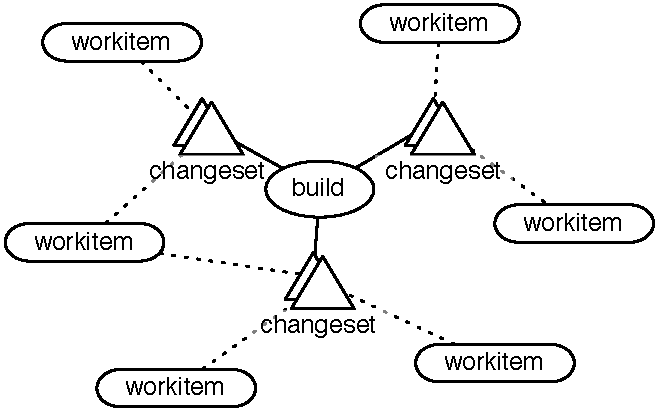
\includegraphics{figures/buildworkitem}}% The larger image 
	
  \centering
  \subfloat[Relationship among Builds, Change Sets, Files, and Work Items]{
    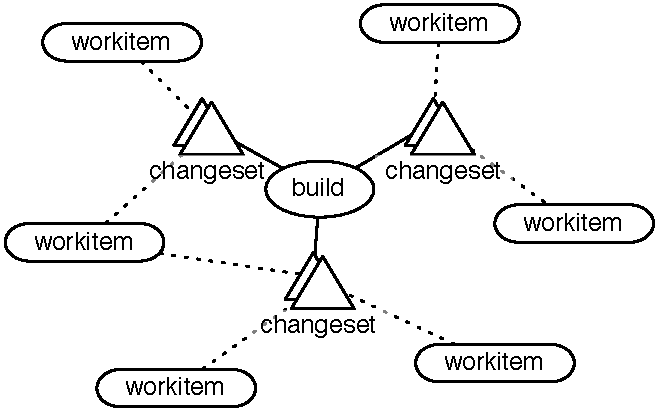
\includegraphics[scale=0.5]{figures/buildworkitem}
    \label{fig:buildworkitem}
  }
  \hspace{8pt}
  \subfloat[Constructing a Coordination Needs Instance]{
  	\raisebox{0.4\ht2-0.5\ht1}{\includegraphics[scale=0.5]{figures/cochangedfiles}} \hfill
    \label{fig:cochangedfiles}
  }
  \hspace{8pt}
  \subfloat[Constructing an Actual Coordination Instance]{
	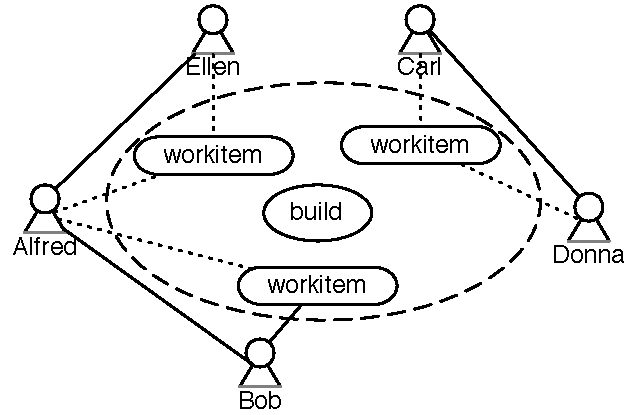
\includegraphics[scale=0.5]{figures/buildsn}
     \label{fig:buildsn}
  }
  \caption{Conceptualizing Socio-technical Congruence in IBM Rational Team Concert}
  \label{fig:constructing}
\end{figure*}

In collaboration with IBM, we acquired a copy of the RTC repository containing data over a one year period.
%between June 2007 and June 2008.
This period of time covers twelve ``milestones'', varying from 1 week to 4 weeks long, during which the RTC team achieved a number of objectives. The end of our data set coincides with a major milestone in which RTC was to be released for open beta testing. 

In addition to quantitative data, we had obtained contextual information about the development team. We also investigated work items, comments, and reports available on the \texttt{jazz.net} web site.

The repository contains build information, work items, comments, change sets, and anonymised author information. We describe the data in more detail below.

\textbf{Work item.} A work item is a description of a unit of work to be done. A work item can be assigned a type of \emph{task}, \emph{enhancement}, or \emph{defect}.
We extracted 2008 unique work items that were relevant to our study.
The same work item may be involved in multiple builds; a total of 9218 non-unique work items were associated with a build across our data set. As our conceptualization focuses on the per-build level, we must consider these non-unique work items.

\textbf{Build.} A build is the process of compiling the software to create a working program.
A build outcome can be an \emph{error}, which indicates that there was either a
compilation error or a test suite error, \emph{OK}, which indicates no
errors, and \emph{Warning}, which indicates that there were warnings
returned by the compiler or the test suites.

A build contains the work from one or more work items, and these work items are not necessarily unique from build to build. The RTC repository does not keep a full record of every build over time, which means that we have more data points for the two most recent milestones compared to earlier in the project.

The RTC repository contains 533 builds, but we consider only builds that contain coordination needs, therefore dropping the number of builds to 214.  We remove 17 builds whose result is Warning because the way that the RTC team treats its Warning builds is dependent on the build. Finally, we remove 7 builds whose types could not be identified. The resulting data set contains 191 builds.

There are three types of builds that we investigate in this study: \emph{continuous builds}, \emph{nightly builds}, and \emph{integration builds}. Continuous builds, which are run regularly by a user, incorporate changes from the local development site, plus known stable components from remote sites.  Nightly builds also incorporate changes from the local site and stable components from remote sites approximately once a day. Integration builds integrate the latest components from every development site. The integration builds are often expected to break due to their large complexity, but errors in continuous and nightly builds are potentially indicative of coordination problems. Our data contains 122 continuous builds, 55 nightly builds, and 14 integration builds.

Because we have a data set of builds over time, we include the date of a build as a variable in our analysis. The build date is conceptualized as the number of days after the first build in our data set.

\textbf{Comment.} A comment is written text authored by a developer that is about a particular work item. Comments are the primary method of transferring information among developers in RTC. Multiple comments may be attached to a single work item. The data subset contains 9323 comments.
%Comments are not threaded---that is, we do not know if a comment specifically references an existing comment in the work item discussion. \\

\textbf{Change set.} A change set is a collection of code changes to a number of files. When a developer updates the repository, all of the files that were changed together are updated in a single change set. A change set is generated by one author only, and is related to exactly one work item. A single work item may contain multiple change sets, and the same change set may occur in multiple builds. There are 3013 change sets in RTC. The number of change sets per work item ranges from 1 to 246. Ninety-five percent of the work items contain 15 or less change sets, and 42\% of the work items contain only one change set.

\textbf{Source code file.} A file contains source code and is included in change sets. Over time, a file may be associated with multiple change sets.

\textbf{Author.} An author is someone who has contributed to RTC. In our conceptualization, we specifically identify an author as meaning someone who has submitted a change set containing modifications to files. Because each change set can be attributed to one author, there are always at least as many change sets as there are authors in a build.


\subsubsection{Distribution of Build Data}

% We illustrate the authors, change sets, work items, and files per build in Figure \ref{fig:buildworkitem}.

Each build involves a number of file authors, change sets, work items, and files. The same author, file, and work item may be involved across multiple builds.
We plot the histograms for each of these entities in Figures \ref{fig:hist_authors}, \ref{fig:hist_changesets}, \ref{fig:hist_workitems}, and \ref{fig:hist_files}.
Most of these distributions, especially the files, are skewed toward the left. 

%We show a scatterplot of the relationships between the number of authors and the number of files per build, as well as the number of authors and the number of work items per build. There is a correlation between authors and files (Spearman $\rho = 0.78$) and no correlation between the number of authors and the number of work items per build (Spearman $\rho=0.056$).

% -------------------------- MOVED TO APPENDIX -------
\begin{figure*}[ht]
\centering

	\subfloat[Authors per Build] {
		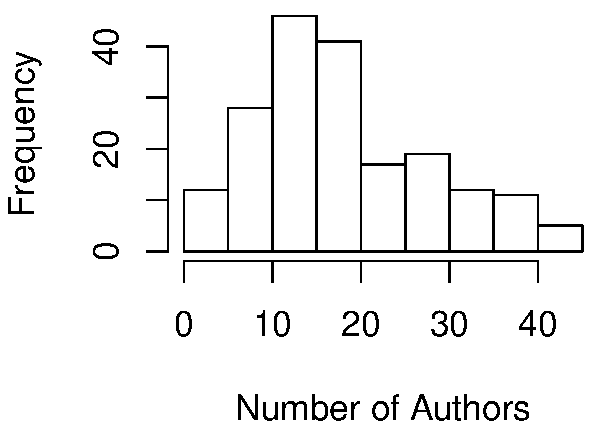
\includegraphics[scale=0.372]{figures/hist_authors_per_build}
		\label{fig:hist_authors}
	}
	\subfloat[Change Sets Per Build] {
		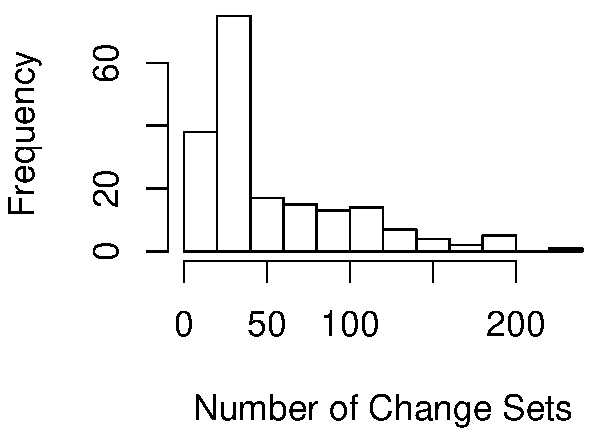
\includegraphics[scale=0.372]{figures/hist_changesets_per_build}
		\label{fig:hist_changesets}
	}
	\subfloat[Work Items Per Build] {
		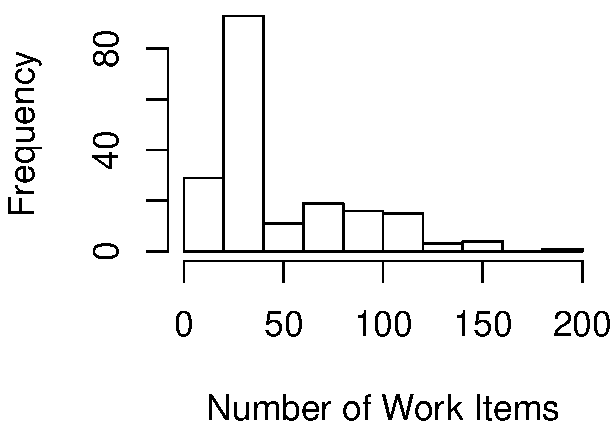
\includegraphics[scale=0.372]{figures/hist_workitems_per_build}
		\label{fig:hist_workitems}
	}	
	\subfloat[Files Per Build] {
		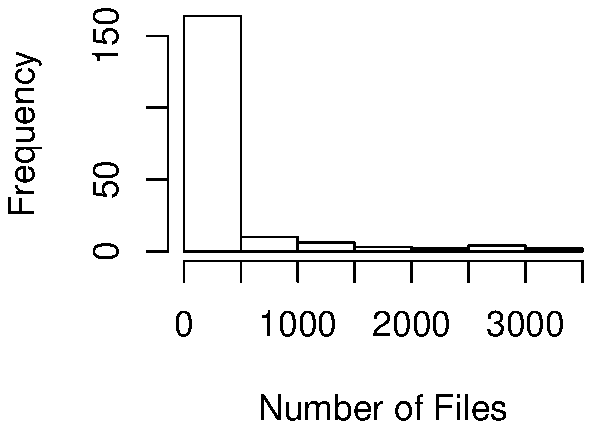
\includegraphics[scale=0.372]{figures/hist_files_per_build}
		\label{fig:hist_files}
	}
	\caption{Distribution of authors, change sets, work items, and files per build}
	\label{fig:entities_per_build}

\end{figure*}
% -------------------------- MOVED TO APPENDIX -------

%\begin{figure}
%\centering
%
%	\subfigure[Authors vs Files] {
%		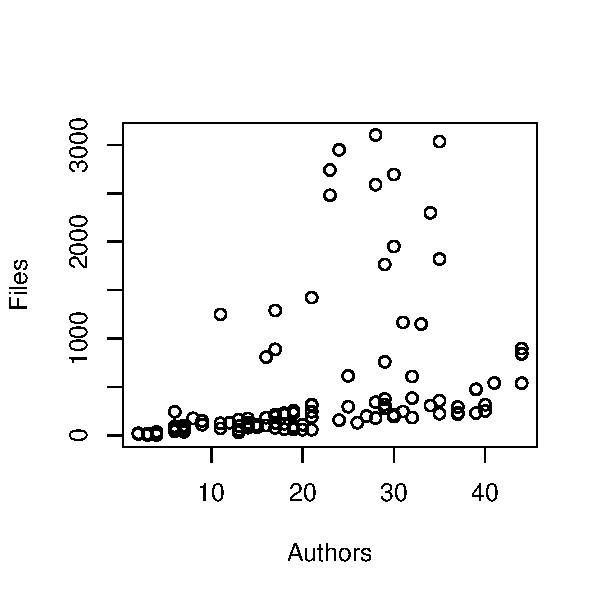
\includegraphics[scale=0.4]{figures/scatter_authors_files}
%		\label{fig:scatter_authors_files}
%	}
%	\subfigure[Authors vs Work Items] {
%		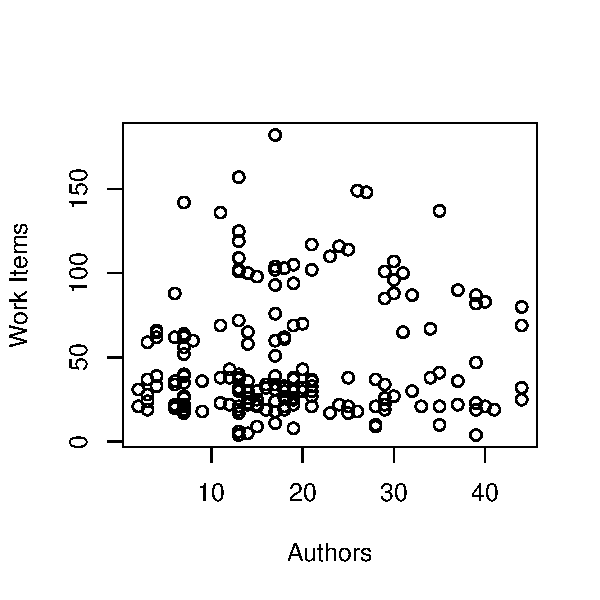
\includegraphics[scale=0.4]{figures/scatter_authors_workitems}
%		\label{fig:scatter_authors_workitems}
%	}
%	\caption{Relationship between build variables per build}
%	\label{fig:relationship_builds}
%\end{figure}

\subsection{Analysis Method}
\label{sec:analysis}

We use the unweighted congruence measure and weighted congruence measure presented in Section \ref{sec:congruence} for our analysis. We explain how we conceptualize congruence in this section.

\subsubsection{Conceptualizing Coordination Needs}

% We conceptualize technical dependencies as files that were changed together in multiple change sets in a build.

Previous studies use various heuristics for determining the dependencies between modules. One conceptualization is based on method call graphs generated by static code analysis, and has been used by Ehrlich \cite{ehrlich2008:gaps}.  Another conceptualization is a ``files-changed together'' heuristic, used by Cataldo \cite{cataldo:cscw:2006}, where the files that were modified in the solution of a change request are considered to be dependent on each other. A third conceptualization is to use experts who manually identify dependencies~\cite{gokpinar2010}.

We decided to construct dependencies based on a variation of the files-changed together heuristic because a ``files-changed together'' heuristic was more reflective of social relationships than a call-graph approach \cite{cataldo:esem:2008}, and best reflected our understanding of the RTC team's work.

We presume that a coordination need between two individuals exists if, minimally, these two individuals change the same file within the same build. In RTC, since only one author can be associated with each file check-in, there are two change sets involved, one associated with each file author. These two individuals should communicate with each other to ensure that the appropriate file dependencies are properly handled before the software is built (Figure \ref{fig:cochangedfiles}).

We generate the coordination needs matrix as follows.

\textbf{1) For each build, we identify every change set included in the build.} Every change set between the previous build and the current build is considered a part of the current build.

\textbf{2) We determine authorship for each file to generate the assignment matrix \emph{A}.} Since each change set has only one author, the author is assigned to every file in that change set. If an author modifies the same file in a different change set, then we add an additional edge for each change set in which the author changed that file.

\textbf{3) We determine the file dependencies in a build to generate the dependency matrix \emph{D}.} We iterate through every change set in the build. Each file is dependent on every other file within a change set. For example, if there are two change sets $C_1$ and $C_2$ in Build 1, with $C_1$ containing files A, B, and C, and $C_2$ containing files A, D, and E, the resulting dependency matrix $D$ would correspond to Figure \ref{fig:cochangedfiles}. In weighted congruence, we add one additional edge for each file pair that exists in each additional change set in that build. Thus, in a Build 2 with change sets $C_3$=\{A,~B,~C\} and $C_4$=\{A,~B\}, the dependency matrix entries in $D$ would be $D_{AB}= 2$, $D_{AC}=1$, and $D_{BC}=1$.

\textbf{4) We calculate the coordination needs as per the coordination needs calculation in Section \ref{sec:stc}.} The diagonals are ignored. When applying weighted congruence, we normalize the coordination needs matrix by taking the highest-ranked edge and dividing every entry in the matrix by that value. This converts each edge to a value between 0 and 1, indicating the relative rank of a coordination need between two individuals in the matrix.

We use this conceptualization because of the explicit relationships between change sets, builds, and authors in RTC. In previous ``files-changed-together'' approaches, multiple files checked in together were associated with multiple authors, whereas in RTC, a change set is authored by one author only. Our conceptualization of coordination needs represents a situation in which two individuals work on a file that are in two different change sets, but are within the same build. Though the file-level changes may not necessarily be to the same lines of code, we presume that multiple changes within a single file are sensitive enough such that each developer working on that file benefits by being informed of every change.

\subsubsection{Conceptualizing Actual Coordination}


We conceptualize actual coordination as communication through comments in the
RTC environment. We treat those who comment on a work item as a group of communicators, and assign weights when individuals comment on multiple work items that others also comment on (Figure \ref{fig:buildsn}).

Though the RTC commenting system allows users to post multiple posts to the same work item, we do not count multiple posts in a single work item as weighted communication.
Since a work item comment can be read by anyone with access to the work item repository, and there is no threading in the work item comments, we cannot assume that there is point-to-point communication from one person directly to another.
In addition, comment communication within the same work item do not correspond to weighted technical dependencies that cross different change sets.

We calculate the actual coordination matrix as follows.

\textbf{1) We identify the comments from the work items involved in a build.} Each build contains a number of change sets, and each change set has an associated work item with comments. For each work item, we include every comment that was posted after the previous build, but before the current build started.

\textbf{2) For each person who commented on a work item, we add a communication edge to every other person who commented on the same work item.} In weighted congruence, add one additional communication edge for each additional work item in which two individuals comment. We do not count weights for multiple comments in a single work item for the reasons discussed above. Thus, if work item $W_1$ contains commenters {A, B, C} and $W_2$ contains {B, C, D}, the resulting entries in the actual coordination matrix $AC$ would be $AC_{AB}=1$, $AC_{BC}=2$, $AC_{CD}=1$, $AC_{AC}=1$, and $AC_{CD}=1$.

\textbf{3) When applying weighted congruence, we normalize the communication network by taking the highest-ranked edge and dividing every edge in the network by that value.} This converts each edge to a value between 0 and 1, indicating the relative rank of comment-based communication between two individuals in the network.

This conceptualization of weighted communication represents the number of people who post a comment to the same work item.

We considered incorporating the RTC development mailing list into communication, but inspection of the mailing list revealed that the developers did not talk about technical issues and that the development list is primarily used for general announcements.

Unfortunately, due to the distribution of the 151 developers in the RTC team, as well as the one-year time period across which our study is conducted, we were unable to collect communication data such as instant messenger or face-to-face communication that we could associate to individual builds. Our concern with this missing data led us to inquire about the use of other forms of media among the team. We learned that although unofficial communication does happen between developers, the RTC team culture requires that the content of unrecorded and private communications be recreated as work item comments for consumption by remote project participants. We still expect that socio-technical congruence will be lower than we might expect from such a team as a consequence.

\subsubsection{Conceptualizing Gap Size}

The gap size in RTC represents a relative distance between the coordination needs and actual coordination. Since the two measurements are not necessarily comparable to each other, we normalize both measures to identify a relative ``rank'' of coordination needs and actual coordination. For example, if there is a coordination need in a build that has many dependencies, intuitively we would want a larger amount of communication around that build rather than on a build with few coordination needs. The gap size calculation identifies this mismatch.

We use the weighted congruence measure to compute the gap size. For each build, we calculate the gap size between each pair with a coordination need using the lack-of-coordination matrix explained in Section \ref{sec:lack}. Because of the normalization, each gap size is a value from $1$ to $-1$, where 1 is a large gap with little or no communication, 0 is full congruence, and -1 is a gap where there is more communication than necessary to fulfill the coordination need. We take the mean of these gap sizes and use this as a variable in a logistic regression model. We also consider an alternative calculation of gap size where we do not punish extra communication and set all values of gap size less than 0 to 0.

\subsubsection{Statistical Analysis Methods}

%Most of our data is highly skewed to the left, meaning that we have a larger proportion of small values than we would expect from a normal distribution. We attempted to fit the data to a log approximation, but found that even with this transformation, the Kolmogorov-Smirnov Test showed significant differences between a normal distribution and our data for both unweighted and weighted congruence. To account for this we use non-parametric statistics to test significance between variables.

To answer Research Question 1, we conceptualize congruence as described in Section \ref{sec:analysis} and test our hypothesis using logistic regression.

Logistic regression is ideal to test the relationship between multiple variables and a binary outcome, which in our study is a build result being either ``OK'' or ``Error''. The presence of many data entities in this project means that we must consider confounding variables in addition to the socio-technical congruence when determining its effects on the probability of build success. Informally, logistic regression identifies the amount of ``influence'' that a variable has in the probability that a build will be successful.

We show the relationship between a variable and the build success probability by plotting the y-axis as the probability. We use probability because we feel that it is more intuitive than odds ratios or logistic functions. If there is a relationship between a variable and the probability of build success, then we should see that as the variable's value increases, the probability also increases. In the probability figures, the solid line is the expected value, and the dashed lines indicate the 95\% confidence intervals.

We run two different logistic regression models: one using weighted congruence, and one using unweighted congruence. We include the following variables: number of files per build, number of authors contributing to the build, number of files in the build, number of work items per build, the congruence, the build type, and the date of the build. We centre and scale each numeric variable.
Because we were concerned about possible interactions affecting our results, we included first-order interaction effects and used backward stepwise elimination to remove variables to keep AIC (Akaike's Information Criterion) low.


% We include also every first-order interaction between these variables to test for possible interaction effects. % Including these interaction effects increased the reliability of the regression model.
%% FIX?
%, increasing the model likelihood ratio $\chi^2$ from 40.04 to 67.15 in the unweighted case $(p = 0)$ and 39.13 to 58.08 in the weighted case $(p = 0)$.

To answer Research Question 2, we calculate the gap size and include this as a variable in our logistic regression model to study the effects on build success probability.

% To answer Research Question 3, we examine in detail overall characteristics of RTC to explore other potential influences that may affect congruence, as well as build results. Data that we examine include the effect of other variables on the build success probability, and the effects of social factors on congruence, such as communication and commenting behaviour.

We use R \cite{R} and the Design package \cite{designR} for logistic regression analysis.

%--------------------------------------------------------------------------------------------------------------


\section{Results}
\label{sec:results}

In the RTC repository, we analysed 191 builds; of these builds, 60 were error builds, and 131 were OK builds. Table \ref{tab:summary} displays summary statistics per build.
Figure \ref{fig:hist_unweighted_congruence} displays histograms for unweighted congruence, and Figure \ref{fig:hist_weighted_congruence} shows histograms for weighted congruence. The histograms compare the frequencies for each type of congruence for all builds, the OK builds, and the error builds only. There are some minor differences between unweighted and weighted congruence values; weighted congruence, for instance, largely reduces the number of ``fully'' congruent situations where congruence is 1.



The congruence values are low on average. The unweighted congruence has a mean value of 0.331, and the weighted measure has a mean value of 0.196, meaning that about one-third and one-fifth of the coordination needs are satisfied by actual coordination, respectively. Over 75\% of the builds have a weighted congruence value of less than 0.25.

\begin{figure}[t]
  \centering
  \subfloat[All builds]{
    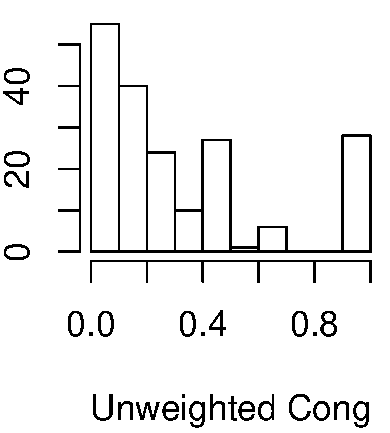
\includegraphics[scale=0.372]{figures/hist_unweighted}
    \label{subfig:hist_nonweighted}
  }
    \subfloat[OK builds]{
    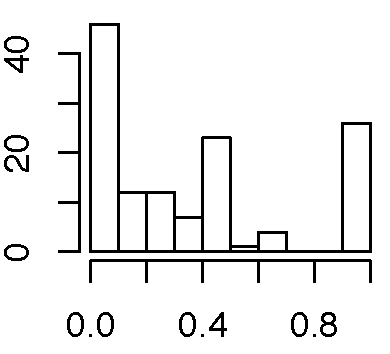
\includegraphics[scale=0.372]{figures/hist_unweighted_ok}
    \label{subfig:hist_nonweighted_ok}
  }
  \subfloat[Error builds]{
	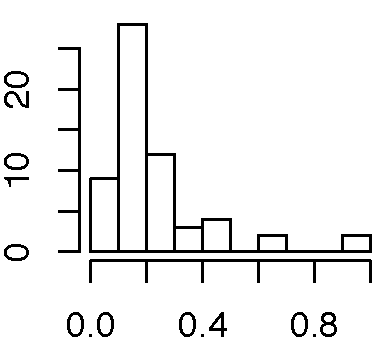
\includegraphics[scale=0.372]{figures/hist_unweighted_err}
     \label{subfig:hist_weighted_err}
  }
	\caption{Distribution of Unweighted Congruence Values}
	\label{fig:hist_unweighted_congruence}
\end{figure}

\begin{figure}[t]
  \centering  
  \subfloat[All builds]{
	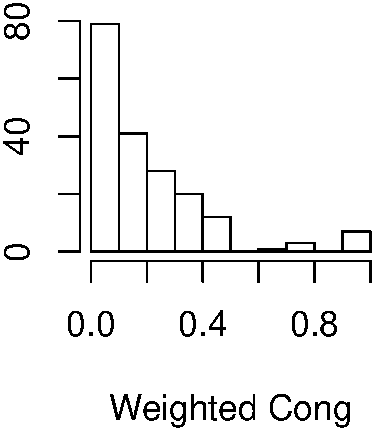
\includegraphics[scale=0.372]{figures/hist_weighted}
     \label{subfig:hist_weighted}
  }
  \subfloat[OK builds]{
    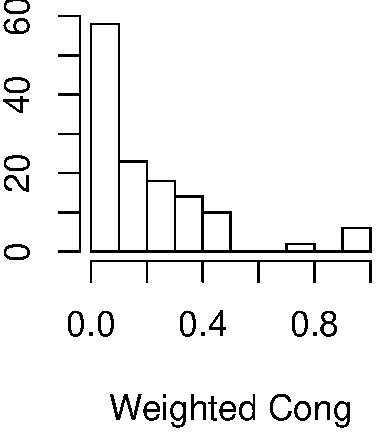
\includegraphics[scale=0.372]{figures/hist_weighted_ok}
    \label{subfig:hist_nonweighted_ok}
  }
  \subfloat[Error builds]{
	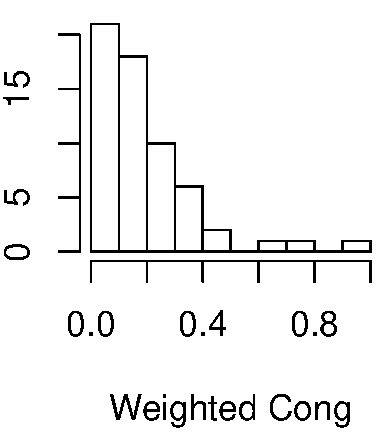
\includegraphics[scale=0.372]{figures/hist_weighted_err}
     \label{subfig:hist_weighted_err}
  }
	\caption{Distribution of Weighted Congruence Values}
	\label{fig:hist_weighted_congruence}
\end{figure}

%              weighted  unweighted     authors       files  workitems        date
%weighted    1.00000000  0.77321937 -0.22499546 -0.13734420 0.04553513  0.02475572
%unweighted  0.77321937  1.00000000 -0.26675774 -0.21972887 0.08265125  0.19178548
%authors    -0.22499546 -0.26675774  1.00000000  0.41240536 0.09800938 -0.30061898
%files      -0.13734420 -0.21972887  0.41240536  1.00000000 0.07767137 -0.20237118
%workitems   0.04553513  0.08265125  0.09800938  0.07767137 1.00000000  0.03615854
%date        0.02475572  0.19178548 -0.30061898 -0.20237118 0.03615854  1.00000000


%We examined data for multicollinearity using variance inflation factor (VIF)~\cite{davis1986}.
%%A high VIF value suggests multicollinearity may exist among the variables, and a low VIF value suggests a lack of multicollinearity.
%% We create separate models for unweighted congruence (Table \ref{tab:vif-unweighted}) and weighted congruence (Table \ref{tab:vif-weighted}).
%In both weighted and unweighted congruence models, there is a significant risk of multicollinearity between authors and change sets.
%We choose to remove change sets from our models because, due to the enforced processes in RTC, we know that there is exactly one author per change set, and therefore, in a build, there is always at least as many change sets as authors, and that removing change sets has no bearing on dependencies as dependencies are calculated at the file level.
%% Removing the change sets reduces the multicollinearity risk.

%Recalculating the VIF indicates that the values are reduced in line with the other variables.
% Model II in Tables \ref{tab:vif-unweighted} and \ref{tab:vif-weighted} illustrate the model without change sets, and shows a reduced risk of multicollinearity between the remaining variables.
% Consequently, the logistic regression models in the remainder of this paper do not include change sets as a variable.

\begin{table}[t]
\centering
\begin{tabular}{l|rrrr}


 & Min & Median & Max & Mean\\\hline
Authors & 2 & 17 & 44 & 18.62\\
Files & 5 & 131 & 3101 & 342.3 \\
Change Sets & 4  & 34  & 226 & 54.2\\
Work items & 4 & 34  & 182 & 48.3 \\
Build date range (days) & 0  & 345  & 361 & 319.2 \\
Unweighted cong. & 0  & 0.21  & 1 & 0.331 \\
Weighted cong. & 0 & 0.15  & 1 & 0.196\\
Gap size & -0.083 & 0.190 & 1.00 & 0.317 \\
\hline
\end{tabular}
\caption{Summary statistics}
\label{tab:summary}
\end{table}

\begin{table}[t]
\begin{center}
\begin{tabular}{l|rrrrrr}


 & 2. & 3. & 4. & 5. & 6. & 7. \\ 
  \hline
   1. Weighted & 0.77 & -0.22 & -0.14 & -0.12 & 0.05 & 0.02 \\ 
   2. Unweighted  &-- & -0.27 & -0.22 & -0.33 & 0.08 & 0.19 \\ 
   3. Authors &  & --& 0.41 & 0.76 & 0.10 & -0.30 \\ 
   4. Files &  &  & --& 0.37 & 0.08 & -0.20 \\ 
   5. Change sets &  &  &  &  --& 0.02 & -0.38 \\ 
   6. Work items  &  &  &  &  &  --& 0.04 \\ 
   7. Build date &  &  &  &  &  & -- \\ 
\hline

\end{tabular}
\end{center}
\caption{Pairwise Correlation of Variables per Build}
\label{tab:pairwise}
\end{table}

We calculated pairwise correlations between the variables weighted congruence, unweighted congruence, number of authors, number of files, number of change sets, number of work items, and build date (Table \ref{tab:pairwise}). There is a strong correlation between weighted and unweighted congruence, which is expected; a strong correlation between change sets and authors; and a weak correlation between authors and files. To avoid multicollinearity problems in our data, we choose to remove change sets from our logistic regression analysis because, due to the enforced processes in RTC, we know that there is exactly one author per change set, and thus there is at least as many change sets as authors per build. Note that weighted congruence and unweighted congruence do not appear in the same model and are thus not subject to multicollinearity problems.

To assess the fit of the logistic regression models, we use the Nagelkerke pseudo-$R^2$ and AIC. $R^2$ shows the proportion of variability explained by the model, and AIC is a measure of how well the model fits the data. Ideally, $R^2$ is high and AIC is low. Our current model contains 19 variables and has an $R^2$ of 0.581 and 0.548 for unweighted and weighted congruence models respectively. We compared our model in Table \ref{tab:models} to a model containing every first-order interaction effect with 27 variables and a model that contains the 7 main effects only (in Table \ref{tab:logr_maineffects}). We found that 19 variables is optimal and that removing further variables lowered the $R^2$ value while raising the AIC.

We observe also that the unweighted congruence model and the weighted congruence model are very similar, with a difference in Nagelkerke $R^2$ of only 0.030.

\begin{table}
\begin{center}
\begin{tabular}{l|r|rr|rr}

             & & \multicolumn{2}{c|}{Unweighted} & \multicolumn{2}{c}{Weighted} \\
Model                  & Variables    & AIC & $R^2$                       & AIC & $R^2$                      \\ \hline
Every interaction  & 27  & 188.6 & 0.595 & 196.7 & 0.559 \\
Main effects only & 7   & 213.2 & 0.269 & 214.2 & 0.263 \\
\textbf{Our model}         & \textbf{19}  & \textbf{175.8} & \textbf{0.581} & \textbf{183.4} & \textbf{0.548} \\
\hline
\end{tabular}
\end{center}
\caption{Model comparison}
\label{tab:models}
\end{table}



% To assist with evaluating the fit of our models, we compared the logistic regression models with the main effects only to the models that included the interaction effects. To evaluate their performance, we used bootstrapping \cite{harrell2001} for each model and plot the results of  the predicted model versus the actual results (Figures \ref{fig:calibrate}). \texttt{Appa}, which stands for apparent validity, provides an optimistic estimate of model performance, and \texttt{bias-corrected} indicates a non-parametric calibration curve estimated from the predicted values. \texttt{Ideal} indicates that the predicted model fits the actual data. We observe that the models with main effects must correct strongly for bias and do not fit as well as the model that includes interaction effects.






% latex table generated in R 2.11.0 by xtable 1.5-6 package
% Thu Jul 29 14:02:07 2010



\subsection{Effects of Congruence on Build Result}
\label{sec:congruence_effect_build_result}


\begin{table*}
\begin{center}
\begin{tabular}{l|rrr|rrr}
 & \multicolumn{3}{c|}{Unweighted} & \multicolumn{3}{c}{Weighted} \\\hline
Variable & Coef. & S.E. & \emph{p} & Coef. & S.E. & \emph{p} \\
	\hline
Intercept                   &  -0.5459 &   0.4663 & 0.2417 &    0.3289 &    0.4729 &   0.4867 \\
\textbf{Congruence}              &   \textbf{6.3410} &   \textbf{1.6262} & \textbf{**0.0001} &    3.6699 &    2.3013 &   0.1108 \\
\textbf{Authors}                     &  \textbf{-1.9759} &   \textbf{0.5310} & \textbf{**0.0002} &   \textbf{-2.0176} &    \textbf{0.5802} &   \textbf{**0.0005} \\
\textbf{Files}                       &  \textbf{-1.0734} &   \textbf{0.4561} & \textbf{*0.0186} &   \textbf{-1.1169} &    \textbf{0.5099} &   \textbf{*0.0285} \\
Work~items                   &  -0.1456 &   0.2355 & 0.5363 &   -0.1365 &    0.2343 &   0.5602 \\
\textbf{Build type=I}                      &   \textbf{2.1533} &   \textbf{1.0526} & \textbf{*0.0408} &    1.2777 &    1.0172 &   0.2091 \\
Build type=N                      &   4.6833 & 200.7587 & 0.9814 &    2.7593 &  192.5236 &   0.9886 \\
Build date                   &  -0.6560 &   0.6709 & 0.3282 &   -0.1352 &    0.7133 &   0.8497 \\
\textbf{Congruence * Build type=I}     &  \textbf{-9.2151} &   \textbf{2.5572} & \textbf{**0.0003} &   \textbf{-6.2748} &    \textbf{2.9664} &   \textbf{*0.0344} \\
Congruence * Build type=N     &  -7.7308 &  91.8053 & 0.9329 &   -7.2024 &  188.1811 &   0.9695 \\
Congruence * Build date  &  \textbf{-5.1266} &   \textbf{1.9290} & \textbf{**0.0079} &   \textbf{-5.5670} &    \textbf{1.9760} &   \textbf{**0.0048} \\
Authors * Build type=I            &   1.2688 &   0.7028 & 0.0710 &    1.1852 &    0.7370 &   0.1078 \\
Authors * Build type=N            & 105.4123 & 535.8792 & 0.8441 &  103.0155 &  521.0808 &   0.8433 \\
Authors * Build date         &  -0.6061 &   0.3616 & 0.0937 &   -0.6004 &    0.3576 &   0.0932 \\
Authors * Files             &   0.7663 &   0.4289 & 0.0740 &    0.4979 &    0.5232 &   0.3414 \\
Files * Build type=I              &   1.0920 &   1.1838 & 0.3563 &    1.7042 &    1.4099 &   0.2267 \\
Files * Build type=N              & -37.9274 & 199.2314 & 0.8490 &  -36.5156 &  192.3382 &   0.8494 \\
\textbf{Work~items * Build date}       &   \textbf{0.8040} &   \textbf{0.3003} & \textbf{**0.0074} &    \textbf{0.8909} &    \textbf{0.3466} &   \textbf{*0.0102} \\
\textbf{Build type=I * Build date}          &   \textbf{2.6442} &   \textbf{0.7678} & \textbf{*0.0006} &    \textbf{1.8627} &    \textbf{0.7621} &   \textbf{*0.0145} \\
Build type=N * Build date          &  84.7252 & 344.8129 & 0.8059 &   84.3117 &  341.4988 &   0.8050 \\
	\hline
Model likelihood ratio & 101.92 & $p \approx 0$ & $R^2=0.581$ & 94.36 & $p \approx 0$ &	$R^2 = 0.548$ \\
& \multicolumn{3}{c}{191 observations} & \multicolumn{3}{c}{191 observations} \\
\multicolumn{1}{l}{ } & \multicolumn{6}{l}{\scriptsize{Build type is set to continuous}} \\
\multicolumn{1}{l}{\scriptsize{*$p < 0.05$; **$p < 0.01$}} & \multicolumn{6}{l}{\scriptsize{Nagelkerke is used as the pseudo-$R^2$ measure}}
\end{tabular}
\end{center}
\caption{Logistic Regression models predicting build success probability with main and interaction effects}
\label{tab:logr}
\end{table*}


\begin{table*}
\begin{center}

\begin{tabular}{l|rrr|rrr}
 & \multicolumn{3}{c|}{Unweighted} & \multicolumn{3}{c}{Weighted} \\\hline
Variable & Coef. & S.E. & \emph{p} & Coef. & S.E. & \emph{p} \\
	\hline                                                                
	Intercept                &  0.5265 & 0.3040 & 0.0833 &  1.00416 & 0.2754 & 0.0003 \\
	Congruence               &  0.9371 & 0.6807 & 0.1686 & -0.85692 & 0.8544 & 0.3159 \\
	\textbf{Authors}         & \textbf{-0.5702} & \textbf{0.2003} & \textbf{**0.0044} & \textbf{-0.64635} & \textbf{0.2023} & \textbf{**0.0014} \\
	\textbf{Files}           & \textbf{-0.6398} & \textbf{0.2477} & \textbf{**0.0098} & \textbf{-0.70618} & \textbf{0.2571} & \textbf{**0.0060} \\
	Work~items                & -0.1755 & 0.1713 & 0.3055 & -0.13229 & 0.1689 & 0.4335 \\
	Build type=I                   &  0.1693 & 0.4269 & 0.6917 &  0.06128 & 0.4154 & 0.8827 \\
	Build type=N                   &  0.2133 & 0.7791 & 0.7842 &  0.29418 & 0.7811 & 0.7065 \\
	Build date               & -0.1331 & 0.1821 & 0.4649 & -0.11291 & 0.1819 & 0.5349 \\
	\hline
Model likelihood ratio & 40.59 & $p \approx 0$ & $R^2=0.269$ & 39.52 & $p \approx 0$ &	$R^2 = 0.263$ \\
& \multicolumn{3}{c}{191 observations} & \multicolumn{3}{c}{191 observations} \\
\multicolumn{1}{l}{ } & \multicolumn{6}{l}{\scriptsize{Build type is set to continuous}} \\
\multicolumn{1}{l}{\scriptsize{*$p < 0.05$; **$p < 0.01$}} & \multicolumn{6}{l}{\scriptsize{Nagelkerke is used as the pseudo-$R^2$ measure}}
\end{tabular}


\end{center}
\caption{Logistic Regression models predicting build success probability with main effects only}
\label{tab:logr_maineffects}
\end{table*}

To answer Research Question 1, we perform a logistic regression analysis between the variables of the builds and the build outcome (Table \ref{tab:logr}).

% \textbf{Null hypothesis:} There is no significant difference between the congruence value in the population of OK builds and the congruence value in the population of error builds in RTC.

% \textbf{Alternate hypothesis:} There is a significant difference between the congruence value in the population of OK builds and the congruence value in the population of error builds in RTC.

The result of logistic regression indicates that the following effects are significant for both unweighted and weighted congruence models: The congruence~$\times$~build type effect, the congruence~$\times$~build date interaction effect, the number of work~items~$\times$~build date interaction effect, and the build date~$\times$~build type effect. In addition, the number of authors and the number of files are significant main effects, although their coefficients are lower than the interaction effects involving congruence. We also identify unweighted congruence as a significant main effects in the unweighted congruence model.

In the next section we discuss the main effects and interactions effects that involve congruence affecting build probability. We discuss the effects of the non-congruence effects, including the authors, files, work~items~$\times$~date interaction effect and the date~$\times$~nightly~build effect in Section \ref{sec:otherfactors}.

\subsubsection{Effects of interactions involving congruence}
\label{sec:congruenceinteractions}

The type~$\times$~congruence interaction effect, the date~$\times$~congruence interaction, and the type $\times$ date effect are each significant in our model (Table \ref{tab:logr}). We plot in Figures \ref{fig:unweighted_congruence_typeci_age} and \ref{fig:weighted_congruence_typeci_age} the effects of weighted congruence vs. probability of build success at the 10\% date quantile (2008-01-25), at the 25\% date quantile (2008-05-14), the 50\% date quantile (2008-06-07), and the latest build (2008-06-26).


\begin{figure*}
\centering
  \subfloat[ \small{2008-01-25} ]{
    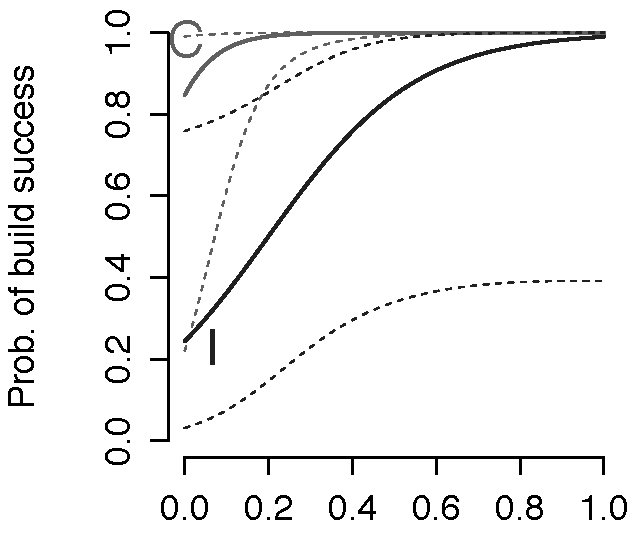
\includegraphics[scale=0.372]{figures/prob_unweighted_age_typeci_q010}
    \label{subfig:prob_unweighted_age_typeci_q010}
  }
  \subfloat[ \small{2008-05-14} ]{
	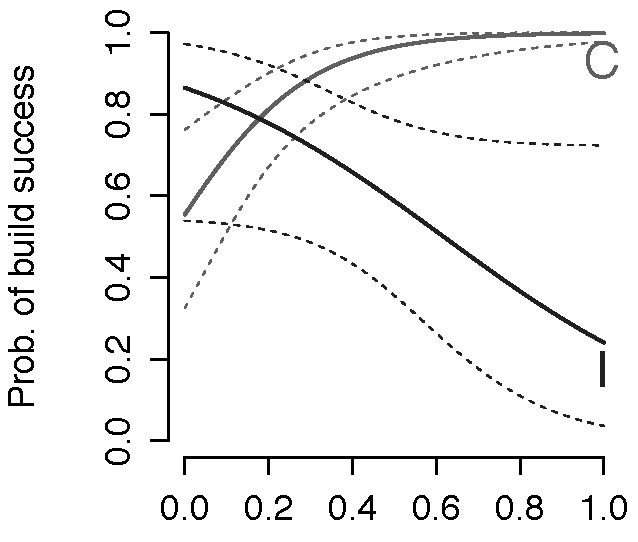
\includegraphics[scale=0.372]{figures/prob_unweighted_age_typeci_q025}
     \label{subfig:prob_unweighted_age_typeci_q025}
  }
  \subfloat[ \small{2008-06-07} ]{
	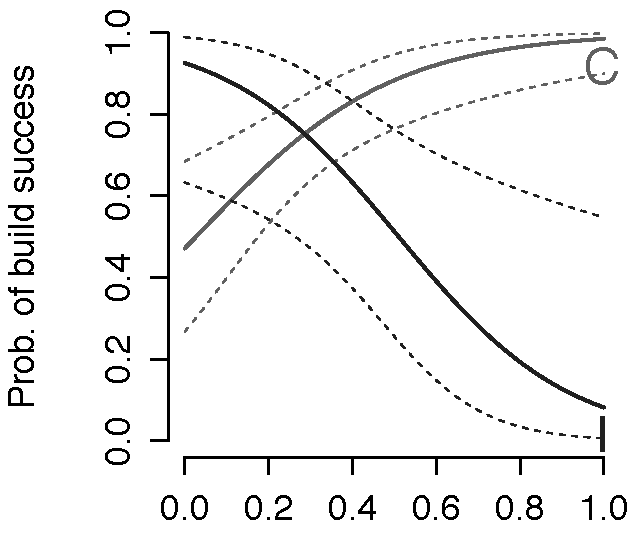
\includegraphics[scale=0.372]{figures/prob_unweighted_age_typeci_q050}
     \label{subfig:prob_unweighted_age_typeci_q050}
  }
  \subfloat[ \small{2008-06-26} ]{
	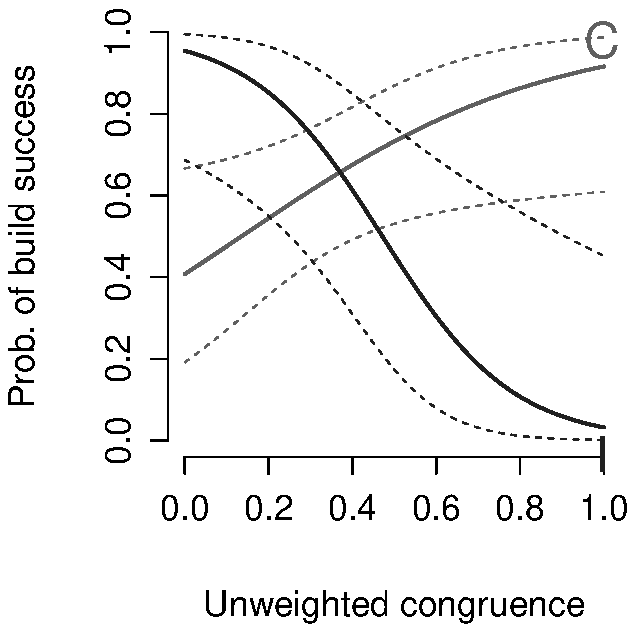
\includegraphics[scale=0.372]{figures/prob_unweighted_age_typeci_q100}
     \label{subfig:prob_unweighted_age_typeci_q100}
  }
  
	\caption{Estimated probability of build success for \emph{unweighted congruence} and \emph{continuous builds C} or \emph{integration builds I}  over time, adjusted to authors $\approx$ -0.156 (17 authors), files $\approx$ -0.352 (131 files), work~items $\approx$ -0.399 (34 work items)}
	\label{fig:unweighted_congruence_typeci_age}
\end{figure*}

\begin{figure*}
\centering
  \subfloat[ \small{2008-01-25} ]{
    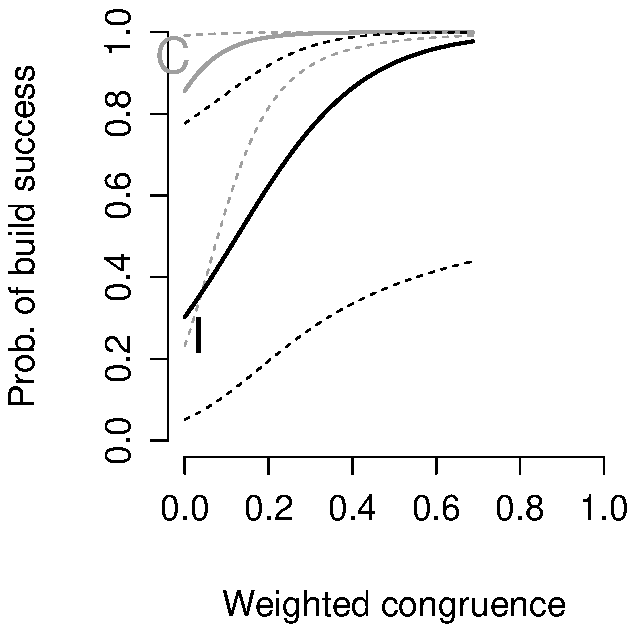
\includegraphics[scale=0.372]{figures/prob_weighted_age_typeci_q010}
    \label{subfig:prob_weighted_age_typeci_q010}
  }
  \subfloat[ \small{2008-05-14} ]{
	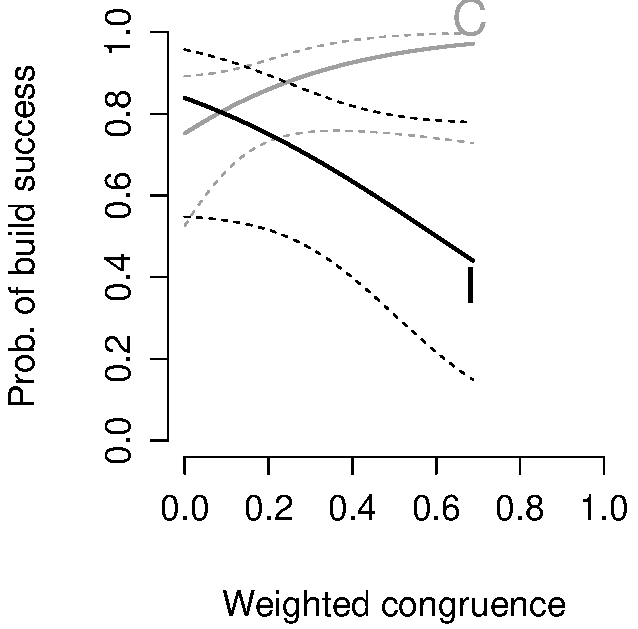
\includegraphics[scale=0.372]{figures/prob_weighted_age_typeci_q025}
     \label{subfig:prob_weighted_age_typeci_q025}
  }
  \subfloat[ \small{2008-06-07} ]{
	\includegraphics[scale=0.372]{figures/prob_weighted_age_typeci_q050}
     \label{subfig:prob_weighted_age_typeci_q050}
  }
  \subfloat[ \small{2008-06-26} ]{
	\includegraphics[scale=0.372]{figures/prob_weighted_age_typeci_q100}
     \label{subfig:prob_weighted_age_typeci_q100}
  }
  
	\caption{Estimated probability of build success for \emph{weighted congruence} and \emph{continuous builds C} or \emph{integration builds I}  over time, adjusted to authors $\approx$ -0.156 (17 authors), files $\approx$ -0.352 (131 files), work~items $\approx$ -0.399 (34 work items)}
	\label{fig:weighted_congruence_typeci_age}
\end{figure*}

% The weighted and unweighted congruence models are very similar, and the effects on the variable for both models are the same. Consequently, we plot only weighted congruence probability plots to save space.


%We examine the relationship between congruence and build type on the build success probability using plots for each type of build across the life of the project. Our data contains 122 continuous builds, 55 nightly builds, and 14 integration builds. 

For continuous builds in weighted congruence (Figures \ref{fig:weighted_congruence_typeci_age}, in grey), an increase in congruence correlates to build success probability. The build date as the project ages appears to decrease the probability of build success for high-congruence builds more than low-congruence builds (Figure \ref{subfig:prob_weighted_age_typeci_q100}). Note that, in the unweighted congruence model (Table \ref{tab:logr}) the effect of unweighted congruence on continuous builds is significant, and that increasing congruence also increases the probability that a continuous build will succeed. However, the effect of weighted congruence in continuous builds is not as large as in unweighted congruence, nor is it considered statistically significant.

For integration builds (Figures \ref{fig:weighted_congruence_typeci_age}, in black), an increase in congruence decreases build success, with the exception of the 2008-01-25 build (Figure \ref{subfig:prob_weighted_age_typeci_q010}). In in our 2008-01-25 build, we see that low congruence leads to low build probability, but high congruence has high build probability. As the project ages, this trend reverses and congruence is clearly inversely related with build success probability (Figure \ref{subfig:prob_weighted_age_typeci_q100}).

The effect of congruence is totally opposite for continuous builds and integration builds in both unweighted and weighted congruence. Based on Figure \ref{subfig:prob_unweighted_age_typeci_q100}, increasing unweighted congruence significantly improves the continuous build success rate. However, increasing both types of congruence significantly decreases the integration build success rate.

% Nightly builds (Figures \ref{fig:weighted_congruence_typen_age}), are the most successful types of builds in RTC, and tend to succeed regardless of the congruence levels. % However the nightly builds also suffer from very wide confidence intervals, suggesting that a lack of data may have had an influence.

% The 95\% confidence intervals, indicated by the dashed lines and \ref{fig:weighted_congruence_summary} are extremely large. As congruence increases, the uncertainty of the effect on the probability of build success increases, suggesting that the relationship between congruence, type, and build success probability is vulnerable to being affected by other variables or random error. 


%For comparison, we illustrate in Figure \ref{} the effects of weighted congruence on build success using the same parameters, in which there is no significant interaction effect. We see a slight increase in build success when increasing weighted congruence in continuous builds (Figure \ref{subfig:prob_weighted_typeC}), but the confidence intervals also increase, decreasing the reliability. Both nightly builds (Figure \ref{subfig:prob_weighted_typeN}) and integration builds (Figure \ref{subfig:prob_weighted_typeI}) suggest no relationship between weighted congruence and build success probability.

%\begin{figure*}
%  \subfigure[ \small{2008-01-25} ]{
%    \includegraphics[scale=0.372]{prob_unweighted_age_typec_q010}
%    \label{subfig:prob_unweighted_age_typec_q010}
%  }
%  \subfigure[ \small{2008-05-14} ]{
%	\includegraphics[scale=0.372]{prob_unweighted_age_typec_q025}
%     \label{subfig:prob_unweighted_age_typec_q025}
%  }
%  \subfigure[ \small{2008-06-07} ]{
%	\includegraphics[scale=0.372]{prob_unweighted_age_typec_q050}
%     \label{subfig:prob_unweighted_age_typec_q050}
%  }
%  \subfigure[ \small{2008-06-18} ]{
%	\includegraphics[scale=0.372]{prob_unweighted_age_typec_q075}
%     \label{subfig:prob_unweighted_age_typec_q075}
%  }
%  \subfigure[ \small{2008-06-26} ]{
%	\includegraphics[scale=0.372]{prob_unweighted_age_typec_q100}
%     \label{subfig:prob_unweighted_age_typec_q100}
%  }
%  
%	\caption{Estimated probability of build success for \emph{unweighted congruence and date}, adjusted to authors $\approx$ -0.156 (17), files $\approx$ -0.352 (131), workitems $\approx$ -0.399 (34), type = cont.}
%	\label{fig:unweighted_congruence_age}
%\end{figure*}

%\begin{figure*}
%  \subfigure[ \small{2008-01-25} ]{
%    \includegraphics[scale=0.372]{prob_unweighted_age_typei_q010}
%    \label{subfig:prob_unweighted_age_typei_q010}
%  }
%  \subfigure[ \small{2008-05-14} ]{
%	\includegraphics[scale=0.372]{prob_unweighted_age_typei_q025}
%     \label{subfig:prob_unweighted_age_typei_q025}
%  }
%  \subfigure[ \small{2008-06-07} ]{
%	\includegraphics[scale=0.372]{prob_unweighted_age_typei_q050}
%     \label{subfig:prob_unweighted_age_typei_q050}
%  }
%  \subfigure[ \small{2008-06-18} ]{
%	\includegraphics[scale=0.372]{prob_unweighted_age_typei_q075}
%     \label{subfig:prob_unweighted_age_typei_q075}
%  }
%  \subfigure[ \small{2008-06-26} ]{
%	\includegraphics[scale=0.372]{prob_unweighted_age_typei_q100}
%     \label{subfig:prob_unweighted_age_typei_q100}
%  }
%  
%	\caption{Estimated probability of build success for \emph{unweighted congruence and date}. adjusted to authors $\approx$ -0.156 (17), files $\approx$ -0.352 (131), workitems $\approx$ -0.399 (34), type = int.}
%	\label{fig:unweighted_congruence_age}
%\end{figure*}

%\begin{figure*}
%  \subfigure[ \small{2008-01-25} ]{
%    \includegraphics[scale=0.372]{prob_unweighted_age_typen_q010}
%    \label{subfig:prob_unweighted_age_typen_q010}
%  }
%  \subfigure[ \small{2008-05-14} ]{
%	\includegraphics[scale=0.372]{prob_unweighted_age_typen_q025}
%     \label{subfig:prob_unweighted_age_typen_q025}
%  }
%  \subfigure[ \small{2008-06-07} ]{
%	\includegraphics[scale=0.372]{prob_unweighted_age_typen_q050}
%     \label{subfig:prob_unweighted_age_typen_q050}
%  }
%  \subfigure[ \small{2008-06-18} ]{
%	\includegraphics[scale=0.372]{prob_unweighted_age_typen_q075}
%     \label{subfig:prob_unweighted_age_typen_q075}
%  }
%  \subfigure[ \small{2008-06-26} ]{
%	\includegraphics[scale=0.372]{prob_unweighted_age_typen_q100}
%     \label{subfig:prob_unweighted_age_typen_q100}
%  }
%  
%	\caption{Estimated probability of build success for \emph{unweighted congruence and date}. adjusted to authors $\approx$ -0.156 (17), files $\approx$ -0.352 (131), workitems $\approx$ -0.399 (34), type = night.}
%	\label{fig:unweighted_congruence_age}
%\end{figure*}




%\begin{figure*}
%  \subfigure[ \small{2008-01-25} ]{
%    \includegraphics[scale=0.372]{prob_weighted_age_typec_q010}
%    \label{subfig:prob_weighted_age_typec_q010}
%  }
%  \subfigure[ \small{2008-05-14} ]{
%	\includegraphics[scale=0.372]{prob_weighted_age_typec_q025}
%     \label{subfig:prob_weighted_age_typec_q025}
%  }
%  \subfigure[ \small{2008-06-07} ]{
%	\includegraphics[scale=0.372]{prob_weighted_age_typec_q050}
%     \label{subfig:prob_weighted_age_typec_q050}
%  }
%  \subfigure[ \small{2008-06-18} ]{
%	\includegraphics[scale=0.372]{prob_weighted_age_typec_q075}
%     \label{subfig:prob_weighted_age_typec_q075}
%  }
%  \subfigure[ \small{2008-06-26} ]{
%	\includegraphics[scale=0.372]{prob_weighted_age_typec_q100}
%     \label{subfig:prob_weighted_age_typec_q100}
%  }
%  
%	\caption{Estimated probability of build success for \emph{weighted congruence} and \emph{build date} for \emph{continuous builds}, adjusted to authors $\approx$ -0.156 (17 authors), files $\approx$ -0.352 (131 files), workitems $\approx$ -0.399 (34 work items)}
%	\label{fig:weighted_congruence_typec_age}
%\end{figure*}

%\begin{figure*}
%  \subfigure[ \small{2008-01-25} ]{
%    \includegraphics[scale=0.372]{prob_weighted_age_typei_q010}
%    \label{subfig:prob_weighted_age_typei_q010}
%  }
%  \subfigure[ \small{2008-05-14} ]{
%	\includegraphics[scale=0.372]{prob_weighted_age_typei_q025}
%     \label{subfig:prob_weighted_age_typei_q025}
%  }
%  \subfigure[ \small{2008-06-07} ]{
%	\includegraphics[scale=0.372]{prob_weighted_age_typei_q050}
%     \label{subfig:prob_weighted_age_typei_q050}
%  }
%  \subfigure[ \small{2008-06-18} ]{
%	\includegraphics[scale=0.372]{prob_weighted_age_typei_q075}
%     \label{subfig:prob_weighted_age_typei_q075}
%  }
%  \subfigure[ \small{2008-06-26} ]{
%	\includegraphics[scale=0.372]{prob_weighted_age_typei_q100}
%     \label{subfig:prob_weighted_age_typei_q100}
%  }
%  
%	\caption{Estimated probability of build success for \emph{weighted congruence} and \emph{build date} for \emph{integration builds}, adjusted to authors $\approx$ -0.156 (17), files $\approx$ -0.352 (131), workitems $\approx$ -0.399 (34)}
%	\label{fig:weighted_congruence_typei_age}
%\end{figure*}

%\begin{figure*}
%  \subfigure[ \small{2008-01-25} ]{
%    \includegraphics[scale=0.372]{prob_weighted_age_typen_q010}
%    \label{subfig:prob_weighted_age_typen_q010}
%  }
%  \subfigure[ \small{2008-05-14} ]{
%	\includegraphics[scale=0.372]{prob_weighted_age_typen_q025}
%     \label{subfig:prob_weighted_age_typen_q025}
%  }
%  \subfigure[ \small{2008-06-07} ]{
%	\includegraphics[scale=0.372]{prob_weighted_age_typen_q050}
%     \label{subfig:prob_weighted_age_typen_q050}
%  }
%  \subfigure[ \small{2008-06-18} ]{
%	\includegraphics[scale=0.372]{prob_weighted_age_typen_q075}
%     \label{subfig:prob_weighted_age_typen_q075}
%  }
%  \subfigure[ \small{2008-06-26} ]{
%	\includegraphics[scale=0.372]{prob_weighted_age_typen_q100}
%     \label{subfig:prob_weighted_age_typen_q100}
%  }
%  
%	\caption{Estimated probability of build success for \emph{weighted congruence} and \emph{build date} for \emph{nightly builds}, adjusted to authors $\approx$ -0.156 (17), files $\approx$ -0.352 (131), workitems $\approx$ -0.399 (34)}
%	\label{fig:weighted_congruence_typen_age}
%\end{figure*}


%\subsubsection{Effect of Number of Work Items}

%Another influence on socio-technical congruence is the number of work items that
%a build is involved in. A work item is of interest in RTC because it represents
%a unit of work. We would expect to see an inverse correlation between the number
%of work items and congruence on the rationale that the more work items that are involved
%in the build, the harder it is for people to coordinate.

%To count the number of work items in a build, we identify the change sets in each build. Each change set is attached to a work item. Our results indicate that the number of work items range from 4 up to 182, with a mean value of 42.54 work items per build. The distribution is highly skewed to the left.

%From our previous models (Tables \ref{tab:logr_unweighted} and \ref{tab:logr_weighted}), which feature the number of work items per build as a variable, there is no significant effect of the number of work items on the build result.

%A correlation test using the Spearman $\rho$ method on the number of work items per build versus unweighted congruence indicated that there was no correlation between the number of work items, and congruence (S = 2.04e+12, p-value~=~0.7869, $\rho = -0.00178$).

%The same correlation test on the number of work items per build versus weighted
%congruence indicated also that there is correlation
%between the number of work items and unweighted congruence (S = 1.88e+12, p-value $<$ 2.2e-16, $\rho = 0.0794$), but because the $\rho$ value is so low, these results are not reliable.

%\begin{figure}
%	\centering
%	\includegraphics[scale=0.5]{figures/boxplot_numworkitems}
%	\caption{Boxplot of Average Number of Work Items Referred to in OK builds and error builds}
%	\label{fig:numworkitems}
%\end{figure}

%We also investigate the relationship between the number of work items and build result. There is a statistically significant difference between the mean number of work items involved in an error build compared to an OK build (W = 61046557, p-value $<$ 2.2e-16) (Figure \ref{fig:numworkitems}).



\subsection{Effect of Gap Size on Build Result}
\label{sec:gapsizeresult}

To answer Research Question 2, we fit a logistic regression model to determine the effect of the mean gap size on the build success probability. The mean gap size appears in Table \ref{tab:summary} and Figure \ref{fig:gapsizes}.
% For error builds, the values range from -0.0405 to 1.0, with a mean of 0.147. For OK builds, the values range from -0.0834 to 1.0, with a mean of 0.391.

%For interest, we adjusted the gap size and limited it to the ranges 0 and 1. A Mann-Whitney test between the gap size and the adjusted gap size illustrates that the difference in means is not significant (W = 18048.5, p = 0.859) and a logistic regression analysis using adjusted gap size instead of gap size with negative values revealed no differences.

We build logistic regression models based on the model in Table \ref{tab:logr} using the gap size measurement. In the interest of saving space, we report only the odds ratio. We retain every significant interaction from our previous weighted congruence logistic regression in Table \ref{tab:logr}.
We compare two different models: Model G1 contains the gap size with weighted congruence as a variable, and Model G2 contains the gap size without weighted congruence.  We do not use unweighted congruence as it is not possible to calculate gap size with unweighted congruence.

The effect of gap size on build result is significant in both models (Table \ref{tab:oddsratio_gapsize}). This indicates that increasing the gap size significantly increases the odds that an OK build will occur, which is the opposite of what we hypothesized (Figure \ref{fig:prob_gapsize_a}). This means that if the gap size is large, the build success probability increases.

%\begin{figure}
%	\centering
%  \subfigure[Gap Size (H1)]{
%	\includegraphics[scale=0.55]{prob_gapsize_5a}
%	\label{subfig:prob_gapsize_a}
%  }
%  \subfigure[Gap size (H2)]{
%	\includegraphics[scale=0.55]{prob_gapsize_6b}
%     \label{subfig:prob_gapsize_6a}
%  }
%	\caption{Effect of Gap Size on build success (authors = 17, files = 131, change sets = 34, type = continuous, and weighted cong = 0.1446)}
%	\label{fig:prob_gapsize_a}
%\end{figure}

% latex table generated in R 2.11.0 by xtable 1.5-6 package
% Mon Sep 13 10:39:05 2010
\begin{table}[h]
\begin{center}
\begin{tabular}{l|rr}
  \hline
 & Model G1 & Model G2 \\ 
  \hline
Intercept & 0.95 & 1.32 \\ 
  Authors & 0.43 & 0.60 \\ 
  Files & 0.63 & 0.63 \\ 
  Work~items & 0.75 & 0.85 \\ 
  Build type=I & 4.22 & 1.31 \\ 
  Weighted cong & 8.41 & - \\ 
  Gapsize & 7.71 & 8.71 \\ 
  Build date & 1.81 & 0.59 \\ 
  Authors * Build date & 0.40 & 0.74 \\ 
  Work~items * Build date & 2.75 & 1.83 \\ 
  Build type=I * Build date & 3.54 & 2.52 \\ 
  Build type=I * Weighted cong & 0.01 & - \\ 
  Weighted cong * Build date & 0.00 & - \\ 
   \hline
\end{tabular}
\caption{Odds Ratio for Gapsize Models}
\label{tab:oddsratio_gapsize}
\end{center}
\end{table}


\begin{figure}[t]
\begin{minipage}[b]{0.4\linewidth}
	\centering	
	\includegraphics[scale=0.372]{figures/boxplot_meangapsize}
	\caption{Mean Gap Size per Build}
	\label{fig:gapsizes}
\end{minipage}
%\end{figure}
\hspace{0.5cm}
%\begin{figure}
\begin{minipage}[b]{0.4\linewidth}
	\centering
	\includegraphics[scale=0.372]{figures/prob_gapsize_g1}
	\caption{Effect of gap size on build success probability, model G1. }
	\label{fig:prob_gapsize_a}
\end{minipage}
\end{figure}

% Adjusted to authors $\approx$ -0.156 (17), workitems $\approx$ {-0.399} (34), type=cont, weightedCong $\approx$ 0.1446, date $\approx$ 2008-06-07)



\subsection{Social and Technical Factors in RTC Affecting Build Success and Congruence}
\label{sec:otherfactors}

% In light of the results of Research Questions 1 and 2, we perform additional analysis on other variables that may affect the probability of build success.
In light of our results, we examine not only the number of work~items~$\times$~date significant interaction found in Section \ref{sec:congruence_effect_build_result}, but different social and technical factors that may affect congruence
and build success probability to find explanations for the interactions between socio-technical congruence and build success probability in RTC.
Specifically, we examine the effect of build date on work items, coordination around fully-congruent builds and
incongruent builds, and the effects of commenting behaviour on builds.

% After adding the "date" variable, authors * files is no longer significant.
%
%\subsubsection{Effect of Authors and Files on build success probability}

%
%The unweighted~congruence~$\times$~build~type interaction is not the only significant variable affecting build result rate. There is a significant interaction between authors and files in both unweighted and weighted congruence (Table \ref{tab:logr_unweighted}). 

%\TODO[FIX THIS] The scatterplot visualization of this data (Figure \ref{fig:scatter_authors_files}) reveals that though most of the builds involve under 500 files, the number of authors across these builds varies from 2 authors to 44 authors.

%To explore this interaction, we plot the effect of the number of files on the probability of build success for different numbers of authors while holding the other variables at fixed values. We show the unweighted congruence plots in Figure \ref{fig:files_authors_unweighted}. Since the effect of authors $\times$ files on build success probability is similar in the weighted and unweighted congruence cases, we do not show the weighted congruence plots to save space. The baseline for comparison is 35 authors, which we chose because it is the level at which the effect of files on build success probability is not extremely pronounced (Figure \ref{subfig:prob_unweighted_35authors}). We do not include the graphs for weighted congruence for space reasons, but the plots for weighted congruence are almost identical to their unweighted congruence counterparts.

%\TODO[FIX THIS TOO] When the number of files is low---700 and below---having a small number of authors involved in the build increases the chance that the build outcome will be successful (Figure \ref{subfig:prob_unweighted_02authors}). Increasing the number of files drastically decreases the probability of build success (Figure \ref{subfig:prob_unweighted_44authors}). However, as more authors contribute to the build, build success decreases when the number of files is low, but build success increases when the number of files are high.


\subsubsection{Other Effects on Build Success}
\label{sec:effectauthors}

\indent\indent
\textbf{Authors} For both weighted and unweighted congruence, as the number of authors involved in a build increases, the probability that the build succeeds decreases. The build probability is significantly lowered after more than 15 authors are involved in the build (Figure \ref{subfig:prob_weighted_authors_age_q100}). When over 30 authors are involved in the build, the estimated build success probability falls under 10\%.

\begin{figure}[b]
\centering
\subfloat[ \small{Authors} ] {
\includegraphics[scale=0.372]{figures/prob_weighted_authors_age_q100}
\label{subfig:prob_weighted_authors_age_q100}
}
\subfloat[ \small{Files} ] {
\includegraphics[scale=0.372]{figures/prob_weighted_files_age_q100}
\label{subfig:prob_weighted_files_age_q100}
}

\caption{Estimated probability of build success for \emph{authors} and \emph{files}, weighted congruence. Adjusted to work~items $\approx$ -0.399 (34), authors $\approx$ -0.156 (17), files $\approx$ -0.352 (131), w. congruence $\approx$ 0.1446, type = cont, date=2008-06-26}
  \label{fig:weighted_congruence_authors_age}
\end{figure}



\textbf{Files} For both weighted and unweighted congruence, as the number of files involved in a build increases, the probability that the build will succeed decreases (Figure \ref{subfig:prob_weighted_files_age_q100}).

\textbf{Build Date and Work items} The work~items~$\times$~date interaction is significant in both weighted and unweighted congruence. Early in the project, as the number of work items increases, the probability of build success decreases (Figure \ref{subfig:prob_weighted_workitems_age_q010}). As the project ages, this trend reverses and as the number of work items increases, the probability of build success increases as well (Figure \ref{subfig:prob_weighted_workitems_age_q100}). According to the coefficients in Table \ref{tab:logr}, this effect on build success probability is not as strong as the authors main effect or the files main effect.

\begin{figure}[b]
\centering
  \subfloat[ \small{2008-01-25} ]{
    \includegraphics[scale=0.372]{figures/prob_weighted_workitems_x_age_q010}
    \label{subfig:prob_weighted_workitems_age_q010}
  }
%  \subfigure[ \small{2008-05-14} ]{
%	\includegraphics[scale=0.372]{prob_weighted_workitems_x_age_q025}
%     \label{subfig:prob_weighted_workitems_age_q025}
%  }
%  \subfigure[ \small{2008-06-07} ]{
%	\includegraphics[scale=0.372]{prob_weighted_workitems_x_age_q050}
%     \label{subfig:prob_weighted_workitems_age_q050}
%  }
  %\subfigure[ \small{2008-06-18} ]{
	%\includegraphics[scale=0.372]{prob_weighted_workitems_x_age_q075}
     %\label{subfig:prob_weighted_workitems_age_q075}
  %}
  \subfloat[ \small{2008-06-26} ]{
	\includegraphics[scale=0.372]{figures/prob_weighted_workitems_x_age_q100}
     \label{subfig:prob_weighted_workitems_age_q100}
  }
  \caption{Estimated probability of build success for \emph{work items} and \emph{date}, weighted congruence. Adjusted to authors $\approx$ -0.156 (17), files $\approx$ -0.352 (131), w. congruence $\approx$ 0.1446, type = cont}
  \label{fig:weighted_congruence_workitems_age}
\end{figure}


%\begin{figure*}
%\centering
%  \subfigure[ \small{2008-01-25} ]{
%    \includegraphics[scale=0.372]{prob_weighted_authors_age_q010}
%    \label{subfig:prob_weighted_workitems_age_q010}
%  }
%  \subfigure[ \small{2008-05-14} ]{
%	\includegraphics[scale=0.372]{prob_weighted_authors_age_q025}
%     \label{subfig:prob_weighted_workitems_age_q025}
%  }
%  \subfigure[ \small{2008-06-07} ]{
%	\includegraphics[scale=0.372]{prob_weighted_authors_age_q050}
%     \label{subfig:prob_weighted_workitems_age_q050}
%  }
%  \subfigure[ \small{2008-06-26} ]{
%	\includegraphics[scale=0.372]{prob_weighted_authors_age_q100}
%     \label{subfig:prob_weighted_workitems_age_q100}
%  }
%  \caption{Estimated probability of build success for \emph{authors} and \emph{date}, weighted congruence. Adjusted to workitems $\approx$ -0.399 (34), files $\approx$ -0.352 (131), weighted congruence $\approx$ 0.1446, type = cont}
%  \label{fig:weighted_congruence_authors_age}
%\end{figure*}

\subsubsection{Commenting Behaviour by Change Set Authors}
\label{sec:commenting}

As congruence expects those who contribute technical work to a project to also communicate changes, we decided to examine commenting behaviour of change set contributors.
We examine whether a work item related to a change set has a corresponding comment posted by the change set's author. We also identify if the work item/change set pair is involved in an OK build or an Error build. Note that a work item/change set pair can occur in multiple builds. We consider only comments posted before the build was started. These results are shown in Table \ref{tab:changesets_authors}.
The build result rates does not appear to be affected by whether the change set contributor commented: 43\% of the builds resulted in error when the contributor commented, and 41\% of builds resulted in error when the contributor did not comment. A $\chi^2$ test on this table does not show a significant difference between the factors at the 0.05 threshold ($\chi^2 = 3.217$, df = 1, {p=0.073}).
Overall, in 76\% of the change set/work item pairs, the change set contributor also posted a comment in the associated work item.
\begin{table}[t]
\centering
\begin{tabular}{lrrr}
Result & \parbox{0.715in}{\raggedright Change sets w/o comment by contributor\vspace{1pt}} & \parbox{0.715in}{\raggedright Change sets w/ comment by contributor\vspace{1pt}} & Total \\\hline 
OK		& 1278 (14\%) 	& 3956 (43\%) 	& 5234 (57\%) 	\\
ERR		& 908 (10\%) 	& 3076 (33\%)	& 3984 (43\%)	\\\hline
Total 	& 2186 (24\%) 	& 7032 (76\%) 	& 9218 (100\%)	\\
\end{tabular}
\caption{Number of change sets in which a contributor commented in the corresponding work item}
\label{tab:changesets_authors}
\end{table}

% We then examined the amount of communication that occurs over coordination needs between pairs of individuals. Over 95\% of the coordination needs in the project are not satisfied by a corresponding communication edge between the developers.

\subsubsection{Examining Extreme Congruence Values}
\label{sec:extremecongruence}

We are interested in the differences between high-congruence builds and low-congruence builds.
We further this investigation by looking at builds that have extreme values of congruence: zero, where absolutely no coordination needs are satisfied with communication, and one, where every coordination need is satisfied with communication.
%A congruence index of 0 means that absolutely no actual coordination occurs where a coordination need exists.
%A congruence index of 1 means that actual coordination occurs for every coordination need that exists.
We chose to investigate the extreme cases to see if there were differences in the way people coordinated in fully-congruent builds, and in incongruent builds.
Table \ref{tab:congruence_extremes} shows the number of OK and error builds that occurred when congruence was equal to one, and equal to zero. The weighted builds with full congruence are a subset of the unweighted builds with full congruence.

%In our data, 32 builds have both a weighted and unweighted congruence index of 0. Among these builds, 2 of them are error builds and 30 are OK builds. It appears that, even in a situation with with 0 congruence, the majority of these builds appeared to have built successfully.

% We then examine the builds that have a congruence of 1, which suggests ``perfect congruence''. There are 26 builds that have an unweighted congruence index of 1; of these builds, 2 builds are error builds and 26 are OK builds. For weighted congruence, there are 7 builds that have a weighted congruence of 1; 1 build is an error build and 6 are OK builds. The weighted congruence builds are subsets of the unweighted congruence builds.

\begin{table}[t]
\centering
\begin{tabular}{ll|rr}
& & \multicolumn{2}{c}{Congruence} \\\hline
&  & 1 & 0 \\\hline 
\multirow{2}{*}{Unweighted} & OK & 26 & 30 \\
                            & ERR & 2 & 2 \\\hline
\multirow{2}{*}{Weighted} & OK & 6 & 30 \\
                         & ERR & 1 & 2 \\
\end{tabular}
\caption{Number of Builds with Congruence Values 0 and 1}
\label{tab:congruence_extremes}
\end{table}



% \texttt{28  44  55  66  71  76  86  104 123 144 147 164 171 172 176 194 210 222 239 246 248 250 256 268 289 292 313 321 336 337 341 347 354}, 33 builds.



%Weighted congruence \texttt{143 177 190 213 226 283 327}, 7 builds.
%Nonweighted congruence \texttt{5   32  42  43  57  63  64  77  80  93  111 113 143 163 170 177 179 190 213 226 266 269 283 297 324 327 355 356}, 28 builds.
% weighted = 0 \texttt{143 177 190 213 226 283 327},
% weighted error: (177)
% unweighted error: build 177 but also build 93. 


To determine if the presence of commenting affected the builds, we examined the number of comments on work item--change set pairs in builds with extreme unweighted congruence values. Our results are shown in Table \ref{tab:changeset_commenters}. Build success probabilities improve with respect to builds that have no comments, though work items with no comments are in the minority.

Of note is the high number of comments on work items that have zero congruence. This indicates that individuals who have no technical relationship to the work item are commenting on the work item.

\begin{table}[t]
\centering
\begin{tabular}{ll|rr|rr}
& & \multicolumn{2}{c|}{Num. of Pairs} & \multicolumn{2}{c}{Success rate} \\
Congruence &                                & 1     & 0   & 1 & 0 \\\hline 
\multirow{2}{*}{No comments} 	& OK 	  & 42   & 143  &  \multirow{2}{*}{49\%} & \multirow{2}{*}{69\%}  \\
                            	& Error   & 43    & 64   &  & \\\hline
\multirow{2}{*}{Comments} 	& OK 	  & 610  & 445  & \multirow{2}{*}{68\%} & \multirow{2}{*}{69\%}  \\
                         	& Error   & 290   & 199  &  & \\\hline
\multirow{2}{*}{Total} 		& OK		  & 652 & 588 &     \multirow{2}{*}{66\%} & \multirow{2}{*}{69\%}   \\
                       		& Error   & 333  & 263 & &\\
\end{tabular}
\caption{Number of work items-change set pairs with comments and build success probabilities for congruence 0 and 1}
\label{tab:changeset_commenters}
\end{table}

We manually inspected the work items with extreme amounts of congruence, reading the comments for any differences in the content discussed. Unfortunately, there were no obvious qualities between comments made in a build with a congruence of zero, and comments made in a build with a congruence of one. In both builds, individuals discussed technical implementation details, provided updates to colleagues, or requested assistance from colleagues. We are unable to discover root causes of failure without a deeper examination of the technical changes and more knowledge of the RTC context.
% Another observation made from reading the comments is that these work items for the cases where congruence is 0 or 1 do not appear to have strong dependencies on other work items.


\section{Discussion}
\label{sec:discussion}

The concepts illustrated in Conway's Law, as well as previous empirical work on socio-technical congruence lead us to expect that team members must coordinate according to coordination needs suggested by technical dependencies in order to build software effectively.
In this case study, we applied socio-technical congruence to study coordination and its relationship to build success probability in RTC. We applied a modified weighted congruence measurement to study also how the size of a coordination gap affects build success probability, and investigated what social and technical factors in RTC affect congruence and builds.

Overall, we found that the average congruence across builds was very low---only 20--30\% of the coordination needs in the project were fulfilled with actual coordination. Even in the cases where there is zero congruence, the build result was an OK build in over 90\% of the observed cases.

Our first research question asked:
\textbf{Does socio-technical congruence have an effect on build success probability in RTC?}
We found that there was an interaction effect involving congruence and build type on build success probabilities (Section \ref{sec:congruenceinteractions}). For continuous builds, increasing congruence improves the chance of build success in continuous builds and can actually decrease build success probability in integration builds (Figures \ref{fig:weighted_congruence_typeci_age}). High unweighted congruence significantly improves continuous build success probability, and both unweighted and weighted congruence significantly reduce integration build success probability.

Our second research question asked:
\textbf{Does gap size have an effect on build success probability
in RTC?}
The gap size is a representation of whether enough coordination
occurred to fulfill multiple coordination needs. If two developers have multiple dependencies on each other, one would expect them to
coordinate more often as well.
We hypothesized that a small mean gap size would increase the probability of successful builds and that a large mean gap size would decrease the probability of a successful build. Instead, we found that as the mean gap size increases, the build success probability also increases (Figure \ref{fig:prob_gapsize_a}).

Below we discuss the reasons for these observed results based on our knowledge of RTC.

\subsection{Strong Awareness Helps Coordination}

The overall congruence for the majority of builds is low: over 75\% of
builds have a congruence of less than 0.25 (Section \ref{sec:congruence_effect_build_result}).
Despite low congruence, the RTC team is able to successfully build its software in many situations.
The fact that the change set author comments on a work item related to the change set does not appear to affect build results either (Section \ref{sec:commenting}), suggesting that changes do not need to be explicitly communicated for every build.

%Even in co-located continuous builds late in the project, increasing congruence does not appear to affect build success probability as strongly as we might have anticipated (Figure \ref{subfig:prob_weighted_age_typeci_q100}).

When we examined extreme congruence values, we observed 85\% build success probability when weighted congruence is 1 and 93\% build success when weighted congruence is 0 (Section \ref{sec:extremecongruence}).
If socio-technical congruence is a measure of coordination quality in software, and builds rely on coordination quality to be successful, then there must be reasons why builds can succeed even when the congruence is zero.

%The theory of socio-technical congruence proposes that low amounts of congruence result in poor outcomes in coordination-intensive activities. We believe that the reasons for this finding are two-fold.

First, because RTC is a highly-distributed project, the product under development uses a modular design \cite{maccormack2006} and thus is affected less by dependencies. Second, team members in RTC do not conduct all of their coordination through \emph{explicit communication} even though work item inspection and discussion with developers indicate that the RTC corporate culture focuses on the work item as their base for communication. Rather, they use the \emph{shared workspace} that incorporates cues from the environment and from peers in order to address technical issues. Both of these effects may contribute to congruence being lower than expected.

\subsubsection{RTC supports Explicit Communication}

The RTC team members use the RTC environment extensively to communicate with each other. We were informed that RTC team members rarely use private email, and our inspection of the mailing list reveals that its primary purpose is for announcements such as server outages rather than for discussing technical work.

This leaves the RTC work item comment system and instant messaging as methods for communication, as well as the phone and internal face-to-face meetings.
We learned that while face-to-face interaction is efficient for solving local issues, it does not benefit remote teams, and the RTC team as a whole encourages every team member to record face-to-face discussions as comments for the purpose of archiving and sharing information.

However, explicit coordination has a cost. There is evidence that involving too many authors in the same build also reduces the build success when using a weighted congruence conceptualization (Figure \ref{subfig:prob_weighted_authors_age_q100}); the effect for unweighted congruence is similar. The overhead required to coordinate many people may interfere with the ability of the team to build the project successfully, suggesting that there is a limit before a developer is overloaded with information.

\subsubsection{RTC is a Shared Workspace}

The RTC client software helps a developer acquire and maintain \emph{environmental awareness} of what is going on in the project by providing access to a shared workspace. Much of the work is centred around the RTC technical entities, which include plans, source code, work items, and comments.
RTC's awareness mechanisms feature a developer-centred dashboard that reports changes to the workspace, built-in traceability, user notifications, regularly-generated reports, and an optional web browser interface. For example, when a change set is created, it is attached to a work item, thus ensuring that people who are involved with the work item receive notification of this change set. These automatic notifications cut down the amount of explicit communication and allow people to coordinate implicitly.

% Their forty-seven teams are distributed across seven sites, and their ``open commercial'' development model centres around the use of the environment as a coordination mechanism. The public is able to view and contribute to RTC. 

% RTC can also be used in a web browser, meaning that any participant can get the benefits of RTC without installing the client.

Coordinating using the workspace is well-known in the computer-supported cooperative work domain \cite{schmidt1996}. Open-source developers, in particular, coordinate around source code~\cite{bolici:stc:2009} and mailing lists \cite{gutwin2004:awareness,mockus2002:opensource} because there is little opportunity for face-to-face interaction. RTC shares many characteristics with open-source development, such as a distributed team and a transparent development process.

In light of these results, we believe that, using our conceptualization, the RTC team requires a congruence of only 0.2--0.3 for their tasks to be completed.
Much of the need for explicit, point-to-point communication is mitigated by implicit communication and the use of the workspace to coordinate.
We expect that the remaining congruence is covered through the RTC workspace, and through face-to-face communication, instant messenger, and phone communication. Though our congruence value appears low for the RTC team, the coordination in reality may be higher. Future studies should keep in mind that congruence may be lower than expected because of conceptualizations that cannot include every type of coordination in a project.

\subsection{Coordination and Geographic Distribution}

As RTC is a distributed team, geographic distribution has an effect on team performance, though the RTC environment helps mitigate some of these effects \cite{Nguyen:2008Distance}.

We learned from the RTC project that continuous and nightly builds should involve mainly a co-located team, and that integration builds involve multiple components from RTC teams in different locations. Our results suggest that congruence best benefits builds that occur within co-located teams; however, the design of our study does not allow us to draw a firm conclusion about the influence of both co-location and congruence on build success probability.

It appears that involving too many individuals when coordinating the activities of various teams may harm build success due to information overload~\cite{damian:icgse:2007}, especially when the team members are distributed. To negate this effect, development leaders and build managers that have an overall view of the project are suited to coordinate teams to ensure build success \cite{hinds:cscw:2006}.

\subsection{Communication Between Individuals Occurs When Problems Arise}
\label{sec:communicating_problems}

Our results indicate that even when congruence gaps are bridged, there is a high probability that a build still fails.

We have observed that, due to awareness through RTC, the RTC team is able to react to situations with multiple technical dependencies by communicating quickly, a trait that has been previously observed among open-source developers \cite{mockus2002:opensource}. Contributors are likely to comment on their own change sets (Section \ref{sec:commenting}).

The RTC team is aware of builds that require high coordination, and are able to address the situation by coordinating with comments. If a work item was particularly complex during development, a developer will post comments on a work item requesting expertise and informing others about unanticipated problems.
This amount of written communication may not occur in an OK build simply because the level of coordination is not necessary; in essence, not every technical dependency requires explicit coordination to bridge that gap.
There is also a possibility that developers coordinate on difficult builds using methods that are not captured by our conceptualizations such as phone or face-to-face. More study of how developers coordinate under ``problematic situations'' is warranted.

% This would lead to the situation where builds with high coordination needs also have high communication.


\subsection{Project Maturity and Build Success}

We found that early builds exhibited a different type of relationship between congruence and build success probability than later builds (Section \ref{sec:congruenceinteractions}). Over the course of the study, we observed 13 internal milestones; the last milestone in our observed builds was a public beta release for end users.

Build success probability decreased significantly over time for continuous builds and stayed roughly the same for integration builds (Figures \ref{fig:weighted_congruence_typeci_age}).
However, the early builds in the project behaved contrary to later builds in the project (Figure \ref{subfig:prob_weighted_age_typeci_q010} and \ref{subfig:prob_weighted_age_typeci_q010}). The RTC software early in its lifetime is in a state of change. Integration builds are not a priority, and features are being added to the project. This means that dependencies are changing rapidly, as well as the expertise among team members, making it difficult to solidify coordination needs.

In addition to interactions between congruence and type, and congruence and date, we observed a significant interaction effect between build date and work items.
We found that early in the project (Figure \ref{subfig:prob_weighted_workitems_age_q010}), builds with large numbers of work items have a high probability of failing, but late in the project (Figure \ref{subfig:prob_weighted_workitems_age_q100}), these builds succeed. Because the latest release was focused on a public release, a build linked to numerous work items may indicate that a bug is highly problematic or a feature is highly desired, and therefore received more attention. This is similar to the effect discussed with gap size (Section \ref{sec:communicating_problems}), where an error build requires more coordination from involved developers.



%\subsection{Social and Technical Factors In RTC}

%% Our third research question asked, What social and technical factors in RTC affect congruence and build success probability?

%% Our intention was to find factors that could explain the lack of relationship between socio-technical congruence and build success probability, by investigating a number of factors that could possibly affect either the congruence or the build result.

%
%Other factors such as work item usage were involved in influencing build success probability and coordination in RTC. We identified the following factors and their effects.

%As mentioned above, we identified that the type of build is related to the amount of necessary coordination and consequently affects congruence.
%We identified that the number of work items in a build does not affect congruence because work items provide a location in the shared workspace for developers to comment, but that the build date and work item interaction does affect build success probability. Initially, builds involving a large number of work items do not have a high probability of success, but this trend is reversed over time. We believe that this is due in part to increased capabilities to handle a build with a large number of issues filed against it. In addition, the phenomenon of developers coming together to discuss error builds that we discussed in Section \ref{sec:communicating_problems} may also apply to the build date $\times$ work item interaction effect.

%We identified that some features of the RTC
%collaboration environment contribute to enhanced coordination behavior and that
%the communication of emergent members (those not captured in coordination needs
%matrices) may possibly contribute to the success of a build.

%We found that the type of build does make a difference when it comes to the
%amount of coordination and consequently the socio-technical congruence values.
%Both continuous builds and nightly builds had similar levels of congruence, which
%is expected as these builds are done at the team level; these teams tend to be
%co-located. However, integration builds had significantly lower congruence
%values. Integration builds, rather than focusing on code changes, tend to focus
%instead on packaging issues. As each team in RTC is responsible for a package
%that is integrated into the final product, full congruence is not necessary. Rather,
%integration can proceed by coordinating representatives for each package. If a
%particular package has problems, then the representative can go back to his
%development team and resolve the issue. It appears that high congruence is not
%necessary for integration builds.

% Adding date removes the significance of this variable.
%\subsubsection*{People and Files in Builds}

%If congruence was not one of the stronger factors affecting builds, which are a coordination-intensive software development activity, then what other variables affect the build success probability?

%The most significant variable affecting build results is the interaction between files and authors. In RTC, increasing the number of files in a build will increase the chances that the build will result in an error, which is expected.  However if you have a large number of authors, the chance of failure will increase.

%We attribute this to issues of coordination overhead---adding a large number of authors increases the difficulty of coordinating each author's dependencies and thus contributes to the error rate of builds. However, if there are a large number of files, increasing the number of authors after a point (34 people for unweighted congruence, 38 people for weighted congruence) results in an increase in the chance of getting an OK build. It appears that, after a point, the additional authors can help manage the dependencies between the files and create successful builds.

% \subsubsection*{The Work Item World}

% There was no observed relationship between the number of work items in the build and build success.

%We observed that 76\% of the developers that attach their change set to a work item also comment on that work item, suggesting that most developers who post a change set also communicate their changes (Table \ref{tab:changesets_authors}).
%% This means that, as more work items are created, in turn creating coordination needs among people, contributors are not increasing their actual coordination to meet these needs and instead, the communication rises proportionally.
%The traceability implicitly provided with the RTC software encourages the change set author to communicate information about the change set, but does not necessarily require that other interdependent people coordinate as well.
%%While this commenting behaviour increases the amount of communication in a build, it does not necessarily lead to increased actual coordination between those who have coordination needs, especially because comments are broadcasted. 
%These results illustrate two benefits of tracing work items to change sets.
%
%First, connecting a work item to a change set allows a developer to communicate without the effort of discovering who to communicate to.
%Developers are highly concerned about contacting the right people when they make modifications~\cite{desouza2007:awarenessnetwork}, but need to go through involved processes to find appropriate contacts~\cite{nakakoji2010:rdc,desouza2007:awarenessnetwork}.
%
%Second, the open work item comment system allows anyone, including people who are not in the coordination needs network, to contribute to the work item (as observed in Table \ref{tab:changeset_commenters}).
%Many people who are not in a technical dependency with the change set comment on a work item to provide expertise.
%RTC provides a way for a developer to write relevant information without the effort of discovering who is affected by the change.


%Other factors that influenced build success probability included increasing number of
%work items involved in the build, increasing the number of comments on a build,
%and increasing the number of change sets in a build. None of these are
%necessarily surprising---increased complexity will contribute to failure. These
%findings align with related work on defect prediction~\cite{cataldo2009:quality,nagappan2005:churn,yu2002:fault}. These results illustrate
%the fact that congruence does not seem to prevent error builds and that simpler factors may be more accurate predictors of build failure.

%\begin{table*}
%\begin{tabularx}{\textwidth}{l|l|X}
%Variable & Effect & Causes \\\hline
%Integration builds & Low congruence $\rightarrow$ build success & Distance affects communication. Specialists from each team involved in build rather than every person with coordination needs. \\\hline
%Continuous builds  & High congruence $\rightarrow$ build success & Distance affects communication, proximity helps people coordinate builds locally. \\\hline
%Gap size & error build $\rightarrow$ small gap size  & Developers coordinate for builds that may be difficult. \\
%\end{tabularx}
%\caption{Findings}
%\label{ph:findings}
%\end{table*}

\subsection{Improvements to Socio-technical Congruence}
\label{sec:improvements}

Based on these results, we discuss our conceptualizations of congruence, and how we can improve socio-technical congruence as an approach to measuring coordination. This paper takes a step in the direction of exploring the situations of applicability that socio-technical congruence has to software projects. Our study is limited to digital, comment-based communication, but indicates the usefulness of socio-technical congruence in highlighting the relationship between communication, technical dependencies, and work outcomes.

% Conceptualizing congruence in RTC required us to take into account not only previous conceptualizations of congruence, but also an understanding of the entities that the developers work with.

We presented a weighted congruence measure which provides measurements such as gap sizes and relationship strengths that were not available by using unweighted congruence. Although the weighted congruence measure yielded similar results to the unweighted congruence measure, the weighted congruence model appeared to lower the threshold of congruence by smoothing out the index values into a more balanced distribution compared to unweighted congruence (compare Figures \ref{subfig:hist_nonweighted} and \ref{subfig:hist_weighted}).
This led to the unweighted congruence model having a significant main effect on continuous build success, whereas the weighted congruence model did not have such an effect.
This shows that weighted congruence is a more conservative
measure than unweighted congruence. Depending on the objective of the
analysis, the unweighted congruence may represent an upper range of
potential congruence in a project, whereas the weighted congruence
tends to be less likely to report perfect congruence and may represent an average scenario.

%Consequently, the unweighted congruence measure is a less conservative measure than weighted congruence. One may want a less conservative measure if a team is observed to work well together in a way that cannot be represented by the conceptualization.
%Weighted congruence measure is more conservative and is appropriate in projects where contextual information about the team is not known.

% In addition, weighted congruence provides additional information such as normalized weights and gap size.% without sacrificing the capabilities of unweighted congruence.

% Thus, the measure provides additional information without sacrificing the capabilities of unweighted congruence.

% This study also illustrates how a detailed measure of coordination can be analyzed from only a software repository, even without face-to-face communication and other unrecorded communication. Numerous practical and ethical implications arise from collecting detailed information from developers such as face-to-face conversations and instant messenger logs.

However our conceptualization of who should be related to a work item is not complete and can be improved.
Many roles in the project are important, but do not have explicit technical dependencies.
For example, we know that RTC has a build coordinator that handles build issues; this person is not assigned to any change sets.
A person who is not identified as being part of the coordination needs network, but appears in the actual coordination network is called an \emph{emergent person}\cite{damian2007:collaboration}.
We identified people who were coordinating with others even though they were not in the coordination needs matrix.
This was illustrated most clearly by the presence of comments on a build that has a congruence index of 0 (Section \ref{sec:extremecongruence}).
Current congruence conceptualizations ignore people that do not have coordination needs but communicate in the actual coordination network.
Thus one improvement is to incorporate people who are involved in actual coordination, but not in technical dependencies, into the congruence calculation. 

A further improvement to socio-technical congruence measures is to improve the
conceptualization of socio-technical congruence to incorporate indirect
communication, especially the information that a developer receives from the
environment. If environment information is transmitted through the software, then fine-grained logging will capture these automatic notifications and can be incorporated into congruence.

Another improvement would be modelling transitive communication because information often travels to individuals through other individuals. For example, an experienced development leader may receive information from multiple teams and forward information to appropriate individuals. Two individuals with a dependency may be able to satisfy their dependencies by communicating through this development leader.

\subsection{Threats to Validity}
\label{sec:threats}

% As this study is a case study examining the relationship between congruence and build success probability, there are a number of threats to validity.
%Conceptualizing congruence is extremely dependent on the project context and the available data. Variations in conceptualization from project to project may explain the results of our paper.

Socio-technical congruence can be difficult to compare between studies. Conceptualizations, such as technical dependencies and actual coordination, vary from project to project. Some project-specific conceptualizations we used are the build as a measure of success, the fact that only files that are touched by more than one individual qualified as having dependencies on each other, and the work item comments connecting people in a clique.
Because of the context-sensitive nature of socio-technical congruence, especially with respect to the construction of communication and dependencies, it is difficult to apply socio-technical congruence as a benchmark for coordination. Having an understanding of the context of the project is extremely important when interpreting results obtained from socio-technical congruence calculations.

%Some of our counter-intuitive results may have been a result of our congruence conceptualizations as well as the limited data we were able to acquire. 

% We believe that, overall, our values for socio-technical congruence are underestimated compared to the coordination that occurs in reality. This is because coordination needs are overestimated, and actual coordination is underestimated.

Our coordination needs are likely overestimated due to the modular nature of RTC.
As we are studying a distributed project that follows a transparent development process, RTC uses a modular design \cite{maccormack2006} and a change in a file in a change set may not necessarily be dependent on other changes within the same file. 
We observed evidence in our study that the dependencies among change sets as well as the attached work items may not be as strong as we have originally believed.

% A future modification would be to take into account not only file dependencies within change sets, but to also examine source code context to come up with a dependency measure that merges the features of both ``files-changed together'' and source code features such as call graphs.

Our conceptualization of actual coordination underestimates the amount of communication that truly occurs in the project. 
We relied on repository data in RTC and were unable to conceptualize forms of communication such as instant messenger, phone calls, and face-to-face interactions.
Due to geographical distance and time zone differences, the RTC team's primary mode of collaboration is the work item comment system, but we made a number of assumptions about commenting behaviour.

% RTC comments are posted in public, which has two implications in our conceptualization.
First, we assume that everyone involved in the work item reads every comment. Second, we do not take into consideration any additional coordination that may occur from a silent onlooker reading the comments. We believe intuitively that the first effect is greater than the second.
This may help explain part of the effect of the unintuitive gap size result; rather than the gap being actually large in reality, it is large in our conceptualization because actual coordination outside of commenting is not recorded.

% These two effects ultimately mean that our calculated congruence would be lower than what occurs in theory. Future studies of congruence might consider scaling congruence to account for missing data.

Another threat to validity is that our data does not cover every build executed in the lifetime of RTC. RTC does not keep a full archive of build results, and as a consequence, we do not have a full population from which to draw data from. The threats are particularly high for early data points. The large confidence intervals in some of the builds, namely nightly builds, reflect this lack of data, thus we hesitate to draw conclusions based on early builds and nightly builds.

% We have observed, in many of our logistic regression models and probability plots, that the 95\% confidence intervals are large. This means that even though we have observed a particular trend in our study, the results are highly variable and the explanation for the observed effects in our study may in fact be influenced by variables outside the scope of our work. Thus, even though we have observed an interaction effect between unweighted congruence and build type in our study, the effect may not be a strong one that holds in the general case.

Finally, this study is a single case study and the results are not generalizable, nor can they be directly compared to existing studies due to the differences in the projects under examination. However, we believe that this study advances the theoretical and the empirical examination of socio-technical congruence, and raises a number of questions that are worthwhile for future study.


\section{Conclusion}
\label{sec:conclusion}

In this paper, we performed a study of coordination in the IBM Rational Team Concert project using a
socio-technical congruence approach. We applied an unweighted congruence
measurement proposed previously in literature as well as a weighted congruence
approach to RTC in order to discover the effects of congruence on
build results. We found that both unweighted and weighted congruence have similar effects on build success probability. With respect to build success probability, we found an interaction effect between congruence
and build results: if the build type was a continuous build, then increasing the congruence led to an increase in the build success probability. If the build type was an integration build, then increasing congruence actually led to a decrease in the build success probability. We also observed interaction effects between congruence and build date, the number of work items and build date, and build date and build type.

%Project maturity appears to have a significant effect on build success probability and may affect the reliability of congruence in predicting build success probability.

% We believe that this result is valuable since we call into question previous
% research has shown that increasing congruence leads to better outcomes.

%In this paper, we present four results from the case study.

%First, we believe that the awareness mechanisms in RTC help developers \emph{coordinate through indirect communication} in order to build software successfully. This result has two implications: it illustrates the usefulness of awareness mechanisms during software development, and it highlights the need for socio-technical congruence to take into account indirect communication when calculating congruence.

%Second, we observed that explicit communication occurs especially when problems arise. This implies that the awareness mechanisms in RTC such as automatically-generated reports, once again, allows developers in RTC to identify problems, contact the appropriate developers, and contribute to the discussion.


Our study, however, has broader significance than the relationship
between socio-technical congruence and build success probability in RTC.
%We determined two factors that reduce the need for high socio-technical congruence when current measures are used.

First, RTC is a
specialized platform that enhances communication over distance and awareness
of work among developers. We believe that the RTC platform may have had the
effect of maintaining awareness among developers, not only through explicit communication in
comments, but also implicit communication through notifications.

%Our investigation suggests that there may be a ``good enough'' threshold for congruence where even a small amount of coordination may cover a large number of technical dependencies. Even though the congruence in RTC builds was low---between 0.2 and 0.3---the RTC team was able to coordinate successfully on builds and respond to builds that had high coordination needs.

Second, we found that RTC developers react to problem situations. If the software is easily built, then coordination is not strictly necessary---environmental awareness may be enough to allow the team members to coordinate. However, if a build and its work items are complex, then the developers communicate more often.

These findings are significant because they provide empirical evidence that illustrate the applicability of socio-technical congruence, and illustrates that an increase in socio-technical congruence may not always be connected to improvements in software development, depending on the conceptualizations and project context.
Nonetheless, we believe that socio-technical congruence is useful for studying the alignment of social and technical entities and can be used to better understand the relationship between socio-technical collaboration and performance in software development.


%%%%%%%%%%%%%%%%%%%%%%%%%%%%%%%%%%%%%%%%%%%%%%%%%%%
%%%%%%%%%%%%%%%%%%%%%%%%%%%%%%%%%%%%%%%%%%%%%%%%%%%
%%%%%%%%%%%%%%%%%%%%%%%%%%%%%%%%%%%%%%%%%%%%%%%%%%%
%%%%%%%%%%%%%%%%%%%%%%%%%%%%%%%%%%%%%%%%%%%%%%%%%%%
%%%%%%%%%%%%%%%%%%%%%%%%%%%%%%%%%%%%%%%%%%%%%%%%%%%

\startchapter{Do Developers Talk about Change-Sets?}

For all but the most trivial programs, software development today is a collaborative activity. The members of software teams must coordinate and communicate, often intensely, if their projects are to reach a satisfactory conclusion.
Previous research has shown that communication among developers has a profound influence on several aspects of software development~\cite{hinds:cscw:2006,wolf:icse:2009}.

%...but beyond a superficial account of communication gaps, research so far tells us little that we can use.
Despite this acknowledged importance of communication in software teams, our understanding of communication behaviour is still very limited. Ko \emph{et al.}~\cite{ko:icse:2007} point out that developers often require information about the work output of their peers.  We know little about why developers act upon this requirement. What causes developers to seek information in some cases, but not in others? There are a multitude of potential factors: the closeness of their peers' work with their own, the expertise of the developers, their physical proximity, their level of workload, and even, perhaps, the time of day. By identifying which factors actually influence the likelihood that a developer will request information about the events surrounding her, we might better understand the nature of software-centric information-seeking behaviour. This increased understanding allows us to develop improved recommender systems that enable developers to coordinate their activities efficiently.

For this study we decided to investigate information-seeking behaviour around changesets for the purpose of identifying guidelines that can improve the applicability and usefulness of recommender systems. A study of changesets is generic enough to be applicable in many settings, but particular enough to be informative about detailed patterns of behaviour. We report on a field study that used a mixed-methods approach (participant-observation, surveys, and interviews) to understand what technical, social, and process-based factors influence whether a developer will seek information about a changeset or not. We investigated communication in the IBM Rational Team Concert (RTC) project, which is distributed across North America, Europe, and Asia, and in which communication is linked to changeset data. The RTC project presents unique opportunities for research on communication in software teams not only because it takes place within a development environment in which a significant fraction of communication is recorded in technical artifacts, but also because the team is tasked with the goal of developing these artifacts themselves. The challenge of effective team communication is particularly present in the RTC project team. 

% JA: We can always just take out the next para if we need space. It's usually meh.
In the remainder of the paper we present the motivation and background for our study, and then describe our study design.  We present in detail the results of our analysis of the data, and distill a number of technical, process and social factors that we identified as influencing developers' information-seeking behaviour. We conclude by discussing the implications of our findings on the design of collaborative systems. 

\section{Background and Motivation}
\label{sec:rq}

% Introduce IBM RTC and the early works of SEGAL with it.
This research builds upon the growing body of work that studies coordination and communication in software organizations, which have long been recognized as playing central roles in leading software projects to success, e.g.~\cite{kraut:1995coordination,curtis:acm:1988}.  
\vspace{-2pt}

Our research group gained the opportunity to study the IBM Rational Team Concert (RTC) development team and the software artifacts produced by this team over several years. The RTC team maintains and cross-links all of their software and process artifacts using the very tool they produce. Partly due to its distributed nature, and partly due to its open source origins, the team's emphasis on written and archivable electronic communication results in a wealth of data for analysis.
\vspace{-2pt}

Our previous investigations of the RTC project repositories revealed a significant relationship between gaps in communication structures and build success~\cite{wolf:icse:2009}. Therefore we proposed a recommendation system that allows team members to learn about who they should talk with in order to avoid build failures~\cite{schroeter:rsse:2008}. This recommendation system should focus on changesets and analyze significant differences between code dependencies and team communication structure to identify anti-patterns that the developers should attempt to break.
The basis for this principle is derived from Conway's Law~\cite{conway:datamination:1968} and by the model of socio-technical congruence proposed by Cataldo \emph{et al.}~\cite{cataldo:cscw:2006,cataldo:esem:2008}.
The model compares the communication network to the code dependency network and derives insights with respect to productivity from the gaps between those networks.
\vspace{-2pt}

In order to build a good recommendation system, however, one needs to go beyond providing valuable information. As Murphy and Murphy-Hill show~\cite{murphy:rsse:2010}, we need developers to trust the recommender system: delivering the right recommendation at the right time is one important way to build such trust. Unfortunately, recommender systems often fall short on this front, saturating the developer with recommendations they neither need nor want, or presenting recommendations at inappropriate times. It is therefore important to know when developers actually need information, and what factors influence them to seek information. There are many potential factors that could change the likelihood that developers would want to obtain further information, and we do not have a sense, other than our intuition, to learn which factors are actually important and which are not.
\vspace{-2pt}

Related work has examined factors that influence communication among software developers. For instance, while APIs are intended to reduce coordination complexity among development teams, they also introduce barriers that hinder communication between teams by obscuring dependencies~\cite{souza:cscw:2004,desouza:fse:2004}.
Software architecture, organizational structure and project age are also factors that influence communication and the awareness that developers have of each other's work~\cite{cleidson:tse:2011}. 
Processes, in particular, are often used to influence the communication among team members to reduce information overload~\cite{fussell:cscw:1998}, and geographic distance has been shown to affect communication, but its effects vary between projects~\cite{herbsleb:icse:2001,wolf:spip:2008}.
Nakakoji \emph{et al.}~\cite{nakakoji2010:rdc} distilled the current knowledge about communication among developers into a set of guidelines to design tools and processes that facilitate effective expertise communication.
Those studies, and to our knowledge, literature in software engineering in general, only address communication on a project-wide level. However, to fully understand, and thus offer actionable knowledge to developers, we need to know what influences an individual developer's information-seeking behaviour.
We surveyed literature to compile a list of possible information-seeking triggers spanning change-related (such as code metrics), developer-related (such as experience level) and process-related (such as peer reviews) factors.

Therefore we pursue to answer the following \textbf{research question:}
 \emph{What factors influence whether a developer will decide to seek information about a changeset in her project?}


% \newpage%\ \newpage
\section{Study Design}
\label{sec:studydesign}

%We studied the communication behaviour around changesets of the software development team of the RTC project.
To address our research question, we complement our previous analysis of the RTC electronic repositories with rich qualitative data from interviews and observations, considering that much information on a project's lifecycle is not recorded in its repositories~\cite{aranda:icse:2009}. We focused on studying what factors cause a developer to seek information about a changeset, since changesets are the smallest units of change to a project that directly impact other developers.
%as well as having the potential to destabilize a project by introducing further failures.

Our research question called for a mixed methods empirical study. Therefore, we collected data about the team's information-seeking behaviour from three different sources.
First, the first author of this paper (Adrian) was embedded in a subteam of the RTC team as a participant-observer for four months.
Second, we deployed a survey with the entire development team to validate some of the findings from the observations.
Third, we conducted interviews with the developers from one component team to obtain richer information about their communication behaviour.

%\vspace{4mm}
\subsection{Study Setting}
\label{sec:rtc}
 
%(MORE HERE FROM PREVIOUS DESCRIPTIONS OF JAZZ IN OUR PUBS) 
Rational Team Concert is a scalable and extensible team collaboration platform that integrates source code management, issue tracking, and planning tools. The RTC platform uses a client-server architecture, with the server acting as a central data repository.
The team also uses RTC to develop RTC, and in this way RTC is a self-hosting project.
This helps the RTC team become aware of issues with the product before customers.% ANYTHING WE CAN SAY ABOUT ITS CUSTOMER BASE? 
The project follows a large scale iterative development process that emphasizes transparency~\cite{frost:ieeesoftware:2007}.
It defines six-week iteration cycles, which are  separated into planning, development and stabilization activities. A project management committee formulates the goals and features for each release at the beginning of each iteration, and the output of this process is assigned to the teams in the form of work items. The work items and nearly all documentation are publicly available.  %(except for the code repository)

The RTC development team has over 100 developers distributed across multiple sites in North America, Europe and Asia.  The RTC development team is subdivided into several teams that manage a component each, such as the source code system or the web user interface. To communicate with each other, especially across different geographical locations, the developers extensively use RTC's own issue and task management system. A particular characteristic of the RTC development environment---and one that made this study of communication behaviour around changesets possible---are explicit traceable links between work tasks, associated changesets, and developers' online comments about these tasks and changesets\footnote{Changesets in RTC are created in a developer workspace; each changeset consists of several changes to code files.}.

%\vspace{4mm}
\subsection{Data Collection}

We used a mixed methods approach to answer our research question. We obtained data from three sources: participant observation, a survey, and a set of interviews with RTC team members.

\subsubsection{Participant-Observation}

The first author of this paper (Adrian) joined one of the RTC development sites in Europe for a four-month period in the Fall of 2010. He was involved as an intern with this development team helping with minor bug fixes, feature development, and testing, and thus was in a position to directly participate in the project development and communication activities. Our data collection opportunities were thus much richer than in typical observations conducted over shorter periods of time, or that do not involve active participation in the project.  During his period as a participant-observer, Adrian kept a daily activity log, recording any information of relevance to the communication behaviour of his team.

The observation period coincided with the months prior to a major release and during which the team focused on extensive testing rather than new feature development. As such, the majority of our observations are concerned with activities around testing the integration of RTC with other IBM Rational products, and it offered the experience of collaborating with many developers from different teams and across the remote sites. Finally, in the one month following the release, Adrian also participated in the development of a feature for the upcoming version of the product.

The team in which he was embedded had the responsibility to develop the task management and the planning components of RTC. There were ten developers at the site, including two novices that had recently joined the team and eight experienced developers. The team includes RTC's three senior project management members, who play a major role in planning the entire product's architecture and development.

\begin{table*}[th!]
\vspace{1pt}
\centering
\subfloat[Process-related items and quotes]{
\small
\centering
\begin{tabular}{l@{\hspace{7pt}}l@{\hspace{20pt}}r}
\toprule
Survey Items & Interview Quotes (I)/Participant Observation Quotes (O) & Mean Rank\\
\midrule
Release endgame & (O) \emph{``Adrian, in the endgame we only do minimal changes. Is your change minimal?''}& 3.79\\%319\\
To review the change &(I) \emph{``I often lack sufficient understanding of the part of the code I'm reviewing.''}& 5.00\\%311\\
To approve the change &--- & 5.11\\%298\\
Late milestone &--- & 5.14\\%293\\
During iteration endgame &(O) \emph{``Adrian, in the endgame we only do minimal changes. Is your change minimal?''}& 5.42\\%288\\
Obtain a review for the change &(O) \emph{``It is demotivating to get a reject, thus I talk to my reviewer beforehand.''}& 5.55\\%287\\
Obtain an approval for the change &(O) \emph{``I already fixed it, but I  need to convince my team lead to give me approval.''}& 5.72\\%281\\
Related work item has high severity &--- & 6.00\\%246\\
Verify a fix &(I) \emph{``Often I need to ask how I can tell that a change-set actually fixed the bug.''}& 6.37\\%235\\
Topic of work item the change is attached to &--- & 7.64\\%181\\
Priority set by your team lead&--- & 8.55\\%152\\
Role of the committer (e.g. developer) &--- & 9.00\\%145\\
Early in an iteration &(I) \emph{``... there are weeks I sometimes don't talk to my colleagues at all.'''}& 11.24\\%66\\
Early milestone &--- & 12.10\\%60\\%\emph{``''}
\bottomrule
\end{tabular}
\label{tab:sub-process}
}\vspace{0pt}
\subfloat[Developer-related items and quotes]{
\small
\centering
\begin{tabular}{l@{\hspace{5pt}}l@{\hspace{-10pt}}r}
\toprule
Survey Items & Interview Quotes (I)/Participant Observation Quotes (O) & Mean Rank\\
\midrule
Author is inexperienced &(O) \emph{``Adrian, please put me always as a reviewer on you change-sets.''}& 2.60\\%385\\
Author recently delivered sub-standard work&(I) \emph{``She just changed teams and still needs to get used to this component.''}& 3.04\\%335\\
Author is not up to date with recent events &(I) \emph{``After you return from vacation we ensure you follow new decisions.''}& 3.15\\%329\\ 
You do not know the change-set author &(I) \emph{``I'd be very irritated if someone other than [...] would touch my code.''}& 5.09\\%269\\	
Author is currently working with you &(O) \emph{``We sometimes discuss changes we made to brag about a cool hack.''}& 5.56\\%226\\	
Author part of same feature team &--- & 6.00\\%190\\ 	
Author part of your team &--- & 7.00\\%188\\ 		
Worked with author before &--- & 7.77\\%165\\ 			
Busyness of yourself &(I) \emph{``If I see a problematic change-set, I'll ask for clarifications even if I'm busy.''}& 8.05\\%164\\
Busyness of the author &(I) {\small\emph{``If I need to know why an author made that change I just contact him.'' [Even if he is busy.]}}& 8.55\\%147\\
Met in person &(I) \emph{``I've worked with him for 5 years now but never even met him.''}& 9.57\\%117\\
Physical location &(O) \emph{``Here, America or Asia, I don't care, I ping them when they are online.''}& 10.14\\%112\\ 
Author is experienced &--- & 11.00\\%93\\ %\emph{``''}		
Author recently delivered high-quality work &--- & 11.09\\%86\\%\emph{``''}
\bottomrule
\end{tabular}
\label{tab:sub-social}
}\vspace{0pt}
\subfloat[Code-change-related items and quotes]{
\small
\centering
\begin{tabular}{l@{\hspace{0pt}}l@{\hspace{-15pt}}r}
\toprule
Survey Items & Interview Quotes (I)/Participant Observation Quotes (O) & Mean Rank\\
\midrule
Changed API &(O) \emph{``Adrian, why did you change that API?''} [The RTC team avoids changing API.] & 2.84\\%390\\            	
Don't know why code was changed &(O) \emph{``I don't see a reason why you changed that code, you sure you needed to?''}& 3.00\\%348\\ 
Affects frequently used features &(I) \emph{``Before I ok a fix [even to a main feature], I ask if there is a workaround.''} & 4.10\\%325\\ 
Complex code &--- & 4.89\\%289\\	%\emph{``''}
Introduced new functionality &--- & 6.14\\%260\\ %\emph{``''}
Is used by many other methods &(O) {\small\emph{``Why did you fix this part? The bug is not in this part of the code, it is used and tested a lot.''}}& 6.41\\%240\\ 
Your code was changed &(I) \emph{``I'd be very irritated if someone other than [...] would touch my code.''}& 6.42\\%232\\ 
Stable code was changed &(O) {\small\emph{``Why did you fix this part? The bug is not in this part of the code, it is used and tested a lot.''}}& 6.62\\%213\\
Change unlocks previously unused code &--- & 7.42\\%192\\ 
A bug fix &--- & 8.61\\%162\\%\emph{``''}	
A re-factoring &(O) \emph{``I separate a re-factoring from a fix so that people can ask me questions about the fix.''}& 9.15\\%152\\
Frequently modified code was changed &(I) \emph{``I like to know where the `construction sites' of the project are.''}& 10.35\\%118\\ 
Code is used by few other methods &--- & 10.96\\%94\\ 	
Simple code was changed\phantom{abcdefgheabcdefghe} &--- & 12.57\\%58\\   %23 characters	43
%Author recently delivered high-quality work	
\bottomrule
\end{tabular}
\label{tab:sub-technical}
}
\vspace{-10pt}
\caption{This table (in three parts) summarizes the data we collected from our three data sources: 1.) our participant-observer's log-book; 2.) survey responses from 36 developers situated around the world; 3.) interviews with 10 developers.  These items are ranked by their average rank.  Whenever possible, we provided quotes from interviews (I), or quotes from the participant-observation period (O) to exemplify the items.}
\addtocounter{table}{-1}
\label{tab:surveyfactors}
\end{table*}

\subsubsection{Interviews}

We conducted interviews with ten developers of the RTC team to inform our observational findings. The setting for the interviews was slightly unusual, and beneficial from a research perspective, since the first author's participant-observation allowed him to develop working relationships during his stay at the team, and to delve into a discussion of complex communication issues without needing to spend time understanding the basic context of the team.

In the interviews, we requested developers to provide details into their communication dynamics through a narration of ``war stories'' that directly related to communication among developers. ``\emph{War stories}'' are events that left an impression on the respondent. War stories emphasize specific events that they witnessed or took part in~\cite{lutters:ist:2007}; their narrative is particularly powerful at uncovering the elements of the stories that are relevant to the respondents. The interviews lasted between thirty minutes and one hour, and they were conducted at the end of the observation period. 


% \newpage
\subsubsection{Survey}

To complement the insights we obtained from the observations and interviews, we deployed a survey with the entire RTC team at the end of our observation period. The survey was designed iteratively and piloted with a European team, and intended to collect input about which factors increase the likelihood of a developer requesting information about a changeset from the changeset author. The items we included in the survey were in the categories of code-related, developer-related and process-related items. Each category included 14 items, as shown in Table~\ref{tab:surveyfactors}. \emph{Code-change related} items describe the changeset delivered or the code that the changeset modifies or affects. \emph{Developer-related} items relate to
the developers that delivered a changeset, the developer requesting the
information, and their relation to each other. Finally, \emph{process-related} items relate to the development phase in effect when the changeset was delivered, and to items relating to process requirements or practices. For each of the three categories, the survey asked the developers to rank each item in the category according to how strongly it increases their likelihood of requesting information about a changeset. 

We initially formulated our list of items from an analysis of the current literature on coordination and communication, as well as from our own previous research. We then refined the list of items through piloting and discussions with the development team. An initial version of the survey included fifty-nine items; the refined list had forty-two. Besides reducing the number of items in our list, the pilot survey led us to add several process-related items, as well as to change the format of the question (the initial survey had a battery of questions with Likert-scale answers; the final survey asked respondents to rank each item in comparison to the rest in its own category).

We deployed the survey through a web form, and invited the entire distributed RTC development team to participate. We sent a reminder one month later to increase the response rate. We obtained 36 responses to the survey; approximately a 25\% response rate.
Of the 36 respondents, 26 are located in North America, 5 are located in Europe, and 5 are located in Asia. Furthermore, 22 of the respondents are developers, 5 team leads, 5 component leads and project management committee, and 4 respondents withheld their information.

%North America, Europe and Asia






%
%Please rank the triggers according to which is more likely to trigger you requesting information about a changeset.}. Survey rankings by the 36 respondents. The rank is determined by the points which is the sum of the reverse rankings provided by the developers.

\subsection{Analysis} 
For our data analysis, we transcribed the interviews, and then coded both the interviews and the participant-observation notes. From the codes we created categories, which we cross-referenced to the survey rankings. We used an open coding approach, during which we assigned codes to summarize incidents in sentences and paragraphs of the transcribed interviews that relate to our research question.

%We calculated the ranking of the survey items for each category with a points-based system in which we added the reverse ranks given by each developer.
%For instance, if a developer ranks an item to be first in its category, then it is worth 14 points (each category has 14 items).
%In case of changes to the API, the first item in Table~\ref{tab:sub-technical} received 390 points which is the sum of nine developers ranking it first (9 $\times$ 14 = 126 points), eleven developers ranking it second (143 points), two developer ranking it third (24 points), four developers ranking it fourth, four fifth, and one sixth, seventh and ninth each. Four developers did not include this item in their rankings.
%We settled for the sum of reverse rankings because the difference in the trends become reinforced over the mathematically equivalent mean.  In 

We calculated the ranking of the survey items for each category by calculating the mean over all ranks given by developers to a survey item (see Table~\ref{tab:surveyfactors}).
Table~\ref{tab:sparkle} shows the distribution of the rankings for each survey item.

During our analysis, we derived a set of factors affecting communication behaviour based on our list of survey items and qualitative data from our interviews and observations. Whenever possible, we triangulated our findings using all our data sources. We tried to ensure that all of our findings were supported by at least two data sources; none of the findings we report were challenged by any of our data sources. 


%\newpage%\ \newpage
\section{Findings}
\label{sec:findings}

% Introduce the findings
The evidence collected from our survey, interviews, and participant observation allowed us to derive seven factors that affect communication behaviour in software organizations, which we outline below. In the remainder of this section, text in italics refers to survey items that can be found in Table \ref{tab:surveyfactors}. Text in italics and around quotation marks denotes interview fragments.

\begin{figure*}[tb]
\centering
\includegraphics[width=\textwidth]{figures/findingProcess2}
\vspace{-20pt}\caption{The pattern of information-seeking interactions throughout several iterations of a release cycle. Every release cycle consists of a number of iterations; each iteration includes an endgame phase. Changeset-based interactions are more frequent during endgame phases and during the last iteration of the release cycle.}
\label{IterationsFig}
\end{figure*}



\addtocounter{table}{1}
\begin{table}[t!]
\centering
\begin{tabular}{ll}
\toprule
\vspace{-2pt}& Process-related items\\
\midrule
\vspace{-2pt}\includegraphics[height=10px, width=30px]{figures/sparkles/during-release-endgame.pdf} & Release endgame\\
\vspace{-2pt}\includegraphics[height=10px, width=30px]{figures/sparkles/you-need-to-review-a-change.pdf} & To review the change\\
\vspace{-2pt}\includegraphics[height=10px, width=30px]{figures/sparkles/you-need-to-approve-a-change.pdf} & To approve the change\\
\vspace{-2pt}\includegraphics[height=10px, width=30px]{figures/sparkles/late-milestone.pdf} & Late milestone\\
\vspace{-2pt}\includegraphics[height=10px, width=30px]{figures/sparkles/during-iteration-endgame.pdf} & During iteration endgame\\
\vspace{-2pt}\includegraphics[height=10px, width=30px]{figures/sparkles/you-need-a-review-for-a-change.pdf} & Obtain a review for the change\\
\vspace{-2pt}\includegraphics[height=10px, width=30px]{figures/sparkles/you-need-an-approval-for-a-change.pdf} & Obtain an approval for the change\\
\vspace{-2pt}\includegraphics[height=10px, width=30px]{figures/sparkles/related-work-item-has-high-severity.pdf} & Related work item has high severity\\
\vspace{-2pt}\includegraphics[height=10px, width=30px]{figures/sparkles/you-need-to-verify-a-fix.pdf} & Verify a fix\\
\vspace{-2pt}\includegraphics[height=10px, width=30px]{figures/sparkles/topic-of-work-item-the-change-is-attached-to.pdf} & Topic of work item the change is attached to\\ 
\vspace{-2pt}\includegraphics[height=10px, width=30px]{figures/sparkles/priority-of-related-work-item-was-set-from-your-team-lead.pdf} & Priority set by your team lead\\
\vspace{-2pt}\includegraphics[height=10px, width=30px]{figures/sparkles/role-of-committer--e-g--developer--team-lead--intern.pdf} & Role of the committer (e.g. developer)\\
\vspace{-2pt}\includegraphics[height=10px, width=30px]{figures/sparkles/early-in-an-iteration.pdf} & Early in an iteration\\
\vspace{-2pt}\includegraphics[height=10px, width=30px]{figures/sparkles/early-milestone.pdf} & Early milestone\\
\midrule
\vspace{-2pt}& Developer-related items\\
\midrule
\vspace{-2pt}\includegraphics[height=10px, width=30px]{figures/sparkles/change-author-is-inexperienced.pdf} & Author is inexperienced\\
\vspace{-2pt}\includegraphics[height=10px, width=30px]{figures/sparkles/recent-work-of-low-quality.pdf} & Author recently delivered sub-standard work\\
\vspace{-2pt}\includegraphics[height=10px, width=30px]{figures/sparkles/change-author-is-not-up-to-date-with-recent-events.pdf} & Author is not up to date with recent events\\
\vspace{-2pt}\includegraphics[height=10px, width=30px]{figures/sparkles/don-t-know-the-change-author.pdf} & You do not know the change-set author \\
\vspace{-2pt}\includegraphics[height=10px, width=30px]{figures/sparkles/currently-working-with-the-change-author.pdf} & Author is currently working with you\\
\vspace{-2pt}\includegraphics[height=10px, width=30px]{figures/sparkles/change-author-part-of-the-same-feature-team.pdf} & Author part of same feature team\\
\vspace{-2pt}\includegraphics[height=10px, width=30px]{figures/sparkles/team-of-change-author.pdf} & Author part of your team\\
\vspace{-2pt}\includegraphics[height=10px, width=30px]{figures/sparkles/worked-with-change-author-in-the-past.pdf} & Worked with author before\\
\vspace{-2pt}\includegraphics[height=10px, width=30px]{figures/sparkles/busyness-of-yourself} & Busyness of yourself\\
\vspace{-2pt}\includegraphics[height=10px, width=30px]{figures/sparkles/busyness-of-the-change-author} & Busyness of the author\\
\vspace{-2pt}\includegraphics[height=10px, width=30px]{figures/sparkles/met-change-author-in-person.pdf} & Met in person\\
\vspace{-2pt}\includegraphics[height=10px, width=30px]{figures/sparkles/physical-location-of-the-change-author.pdf} & Physical location\\
\vspace{-2pt}\includegraphics[height=10px, width=30px]{figures/sparkles/change-author-is-experienced.pdf} & Author is experienced\\
\vspace{-2pt}\includegraphics[height=10px, width=30px]{figures/sparkles/recent-work-of-high-quality.pdf} & Author recently delivered high-quality work\\
\midrule
\vspace{-2pt}& Code-change related items \\
\midrule
\vspace{-2pt}\includegraphics[height=10px, width=30px]{figures/sparkles/change-modified-API.pdf} & Changed API\\
\vspace{-2pt}\includegraphics[height=10px, width=30px]{figures/sparkles/don-t-know-why-code-was-changed.pdf} & Don't know why code was changed\\
\vspace{-2pt}\includegraphics[height=10px, width=30px]{figures/sparkles/code-affects-frequently-used-features.pdf} & Affects frequently used features\\
\vspace{-2pt}\includegraphics[height=10px, width=30px]{figures/sparkles/complex-code-was-changed.pdf} & Complex code\\
\vspace{-2pt}\includegraphics[height=10px, width=30px]{figures/sparkles/change-introduced-new-functionality.pdf} & Introduced new functionality\\
\vspace{-2pt}\includegraphics[height=10px, width=30px]{figures/sparkles/code-is-used-by-many-other-methods.pdf} & Is used by many other methods\\
\vspace{-2pt}\includegraphics[height=10px, width=30px]{figures/sparkles/your-code-was-changed.pdf} & Your code was changed \\
\vspace{-2pt}\includegraphics[height=10px, width=30px]{figures/sparkles/stable-code-was-changed.pdf} & Stable code was changed\\
\vspace{-2pt}\includegraphics[height=10px, width=30px]{figures/sparkles/change-unlocks-previously-unused-code.pdf} & Change unlocks previously unused code\\\
\vspace{-2pt}\includegraphics[height=10px, width=30px]{figures/sparkles/change-was-a-bug-fix.pdf} & A bug fix\\	
\vspace{-2pt}\includegraphics[height=10px, width=30px]{figures/sparkles/change-was-a-re-factoring.pdf} & A re-factoring\\ 
\vspace{-2pt}\includegraphics[height=10px, width=30px]{figures/sparkles/frequently-modified-code-was-changed.pdf} & Frequently modified code was changed \\
\vspace{-2pt}\includegraphics[height=10px, width=30px]{figures/sparkles/code-is-used-by-a-few-other-methods.pdf} & Code is used by few other methods\\ 
\vspace{-2pt}\includegraphics[height=10px, width=30px]{figures/sparkles/simple-code-was-changed.pdf} & Simple code was changed\\
\bottomrule
\end{tabular}
\vspace{-5pt}
\caption{This table contains the distribution of ranks for each survey item. The leftmost point of each sparkline represents the amount of respondents that ranked the item first; the rightmost point represents the amount that ranked it last (14th). No survey item received the same rank from more than ten respondents.}
\label{tab:sparkle}
\vspace{-20pt}
\end{table}




%\pagebreak
\subsection{Development Mode}

% Introduce development modes
One of the strongest findings from our study was the effect of the development mode that the team is in on its communication behaviour. Developers and managers alike give much importance to the development mode they are in, namely (1) normal iteration, and (2) endgame.

% Normal iteration
The normal iteration mode mainly consists of work that can be planned by the developer. This work tends to be new feature development, or modifications to existing features. Most of the planning for it has been laid out in advance; furthermore, each developer individually knows what features have been assigned to her, and can plan ahead to meet her obligations.
% Endgame
In contrast, the endgame mode mainly consists of work that is coming uncontrollably in short intervals from others. As a result of integration and more intense testing, defects crop up more rapidly and need to be addressed more quickly. Beyond allocating time for endgame activities, there is very little in this development mode that can be planned in advance.

% Cyclical pattern
The RTC team switches between the two modes in each iteration. Of the six weeks of a regular iteration, four weeks are assigned to normal iteration mode and two weeks to endgame. However, as deadlines approach, there are occasional special iterations that consist mostly of endgame-like work. In this manner, the same detailed pattern of alternation between normal iteration and endgame within an iteration is reproduced at a higher level, as shown in Figure~\ref{IterationsFig}.

% Make it clear what the finding is
We identified the same pattern with respect to the amount of changeset-related interactions in the team. We found that the mode in which the team is currently in is an important factor determining whether developers will feel a need to communicate about changesets. Being in endgame mode increases the need for developers to communicate about a changeset, whereas being in normal mode decreases the need to request information about it.

% Participant-observer data
The first author of this paper experienced both modes during his participant-observer time with the RTC team. He joined the team in a release endgame phase, which was characterized by fixing bugs that were reported by testers, and he helped by fixing minor bugs as well as setting up servers for testing. When the team released the project, it switched gears, and in the decompression after the endgame he had the opportunity to develop a feature for the product. The differences in the patterns of interaction between the two modes were distinctly clear, for him and for his peers. During the endgame mode, developers were essentially ``on demand,'' available to fix whatever bugs were discovered. Later, during the normal iteration mode, they experienced far more autonomy and control over their time, and began working on activities that were less demanding of an interaction back-and-forth, and especially less demanding of keeping track of the changesets committed by their peers. In our interviews, developers almost unanimously pointed to the separation of the two types of modes, describing the differences in the type of communication in each, and identifying the autonomous \emph{vs.}~uncontrollable, inside \emph{vs.}~outside influence.

% Some interview data
This is not to say that developers do not communicate while they are in normal iteration  mode, but that the nature of their communication seems to be different. In normal iteration mode, developers communicate less about concrete changesets, but they communicate more about high level ideas: for instance, they raise questions about how a feature fits into the existing architecture or general tactics to implement a feature, about how much of it actually needs to be implemented or can be reused from other libraries, and so forth. Generally, however, the amount of communication decreases in normal iteration mode. As a developer commented in one of our interviews, \emph{``during feature development iterations there are weeks I sometimes don't talk to my colleagues at all.''} 

In contrast, the endgame mode is characterized by bug reports and last minute feature requests---that is, by work coming into every developer's desk uncontrollably. Changesets become first class concerns during this mode because each change threatens the stability of the product: developers need to evaluate whether the changeset actually improves the product instead of making things worse. Therefore, they develop a habit of reviewing each other's changesets to assess the risk they pose to the project's stability.

% Survey data
Our survey data provides significant support for this finding. In Table~\ref{tab:sub-process}, we can see that overall, for the RTC development team at large, there is a greater likelihood to request information during product-stabilizing phases, such as 
\emph{during the release endgame}, and a lesser likelihood to request information when working towards an \emph{early milestone}. The former was ranked as the most important of the process-related items in our survey; the latter was ranked as the least important. All the survey items that refer to a late stage in the iteration or in the project lifecycle were ranked highly, and all the items that refer to an early stage were ranked lowly. This finding resonates especially with the team we interviewed. 

%\begin{note}
%The likelihood that a developer will request information about a changeset increases when the team is in a development mode characterized by uncontrollable work coming from outside.
%\end{note}

%- number 1, 4, 5, 13,14
%- interviews: content changes
%-- sometimes frequency changes
%-- income vs out going
%-- other define vs self defined


\subsection{Perceived Knowledge of the Changeset Author}

% Introduce this as another one of our Big Deal findings
One key determinant for a developer to seek information about a changeset consists of what the developer knows about the background of its author. Several aspects of the author's background seem to be important: the quality of her recent work, her level of experience, and her awareness of recent team events or decisions.

% Sub-standard work
First, these factors are important in part because they point to potential problems with the stability of the product. If a changeset author has \emph{recently delivered sub-standard work}, other developers will want to ensure that the new changeset will not deteriorate their product, and therefore they will try to find more information about it.

% Experience
Similarly, when the author is \emph{inexperienced}, or is not \emph{up to date} with recent team events for any reason, the risk of introducing problems into the product increases. One developer that interacts frequently with a newly founded team told us that \emph{``most of the work that I need to review is of very low quality and needs several iterations before it is up to our standards.''} Novices, generally speaking, face a ramp-up problem that takes a significant amount of time to overcome~\cite{begel:sigcse:2008}. This was the case with Adrian's work, too: his first changesets were subjected to more scrutiny due to his unfamiliarity with the code base.

% Survey data
The survey data backs up these observations. The three top items in Table \ref{tab:sub-social} consist of factors related to an unfavourable perception of the background of the changeset author. In comparison, the two least important items in that table refer to favourable perceptions of said background.

% It's partly about perception and trust
In essence, these items point to the relevance of trust in software development teams. For developers, trust in the skills of their colleagues is important. If this trust is not-established (for instance, if a developer does not know the changeset author), developers are more likely to check the changeset and request information to ensure that the modifications were truly necessary and appropriate. But when trust exists (that is, when the author has a good record of delivering high-quality work, or is known to be an experienced team member), the need to seek information about a changeset decreases. 

%\begin{note}
%It is more likely that a developer will request information about a changeset delivered from an author that recently delivered sub-standard work, or is perceived as inexperienced or unaware of team events and decisions.
%\end{note}


% observation
% no observations
%- experience 1
%- quality of recent work 2
%- up to date 3
%- don't know the author 4
%- experience 13
%- quality of recent work 14
%- role of the committer 12 (process)


\subsection{Common Experience and Location}

Shared work experiences affect the likelihood of information-seeking behaviour in the RTC distributed team. This is partly related to the trust and perception issues discussed above, but also to the establishment of interpersonal relations and to the intertwining work responsibilities and expectations.
\vspace{-2pt}

According to our interviews, this is the case particularly for senior team members. Although they work in a globally distributed team, they have managed to establish personal relationships with developers at many different sites. Through continuous interaction and through social events, they have learned more about each other, and thus feel more comfortable to initiate contact with them. Junior team members, in contrast, know very few of their teammates globally, and since they simply do not have these interpersonal connections with the rest of their team, it is less important to them whether they know the author of a changeset when needing to contact them.
\vspace{-2pt}

Generally speaking, despite the lack of opportunities to build personal relationships with off-site people, for most developers sharing common experiences makes it easier to contact teammates to request information. One team lead told us: \emph{``I have one or two contact people in each team we usually work with whom I ask for information and then often enough get referred to the right person in their team.''}
\vspace{-2pt}

Our participant-observation data confirm this. At one point, Adrian needed to set up and test a specific component in the RTC product. The development team in charge of that component was located on a different site. However, since Adrian had previously had the opportunity to establish relationships with some of the developers of that team through a previous research study, it was easier for him to contact them and ask for help in his setup task.
\vspace{-2pt}

Our survey data corroborate these observations. It suggests that the developers that form relationships (on a personal or work level) with other developers gave more emphasis on previous experiences with them. For instance, it made a difference whether the developers \emph{are currently working together} (Table~\ref{tab:sub-social}). Additionally, whether they have shared work experiences seems to be a more determinant factor than having \emph{met in person} or sharing the same \emph{physical location}.

This last finding would seem to indicate that the RTC team has managed to overcome obstacles created by geographical distance. Developers state that the physical location of a changeset author is not an important factor to seek more information about the changeset. Nevertheless, we should note two things. First, this finding merely points out that developers have no greater need to inform themselves of work output of their remote peers than of their local peers; it says nothing about the ease with which such information is acquired. Second, the RTC team has determined to carry out as many of its interactions as possible through textual, electronic media. This neglects the natural advantages provided by proximity in favour of uniform accessibility of interactions, no matter the physical location of the interlocutors.
\vspace{-2pt}

%\begin{note}
%Recent or shared work experiences eases the act of requesting information from distributed or local developers.
%\end{note}

%- currently working with author 5
%- same feature team 6
%- same team 7
%- worked with before 8
%- met author in person 11
%-- physical location 12


\subsection{Risk Assessment}

A central factor at the heart of the decision to seek information is a concern with the quality of the product and components developed by the team at large. Both managers and developers share this concern. Because of it, every team member is constantly evaluating whether there are significant risks involved in accepting a changeset and including it into the final product. This concern is greatest close to releases or major milestones, and less important when the team is in normal iteration mode.

Developers request information more frequently about changesets that touch on code that has a high customer impact. According to our interviews and observations, code parts with a high customer impact are those that are directly related to frequently used features or changes to the API that might be used by customers to customize the RTC product. In the case of the impact of API changes, there is an extensive knowledge exchange in the jazz.net forums between customers and developers about how to use the API to build extensions to RTC, which gives developers plenty of information about the possible impact of API changes to the customers. Consequently, changesets that modify code that has less impact on the customer are of less concern and less likely to be discussed. For example, when scanning fixes to reported bugs, developers perform a risk assessment to determine whether the bug fix is even needed. In the words of one team member, \emph{``with every tenth bug fix you introduce another bug to the system, so unless the bug does not have a workaround and is something most customers would experience, we give it low priority.''}

The ranking of items in Table \ref{tab:sub-technical} provides additional insights into the kinds of changesets that carry a risk for developers. A \emph{changed API} comes at the top of the list, code that \emph{affects frequently used features} comes third, immediately followed by changes to \emph{complex code}, changes that \emph{introduced new functionality}, and changes to code that \emph{is used by many other methods}.

%\begin{note}
%Developers investigate more carefully those changesets that might have a high impact to the customers or to the stability of the code base, and thus they are more likely to request information about them.
%\end{note}

%- API 1
%- don't know why 2
%- frequent features 3 (customer)
%- complex code 4
%- new functionality 5
%- used by many others 6

%- stable code was changed 8
%- unlock previously unused code 9

%- frequently code was changed 12
%- code is used by few others 13
%- simple code was changed 14


\subsection{Work Allocation and Peer Reviews}

In the later stages of the development cycle, developers have two process-based constraints that prompt them to interact with their peers. First, they need their peers to review their changesets before they are included in the product. Second, they need an approval to start working on a task (a triaging process needs to take place so that developers are allocated to the most important work items).

In the changeset review process, there are two ways the changeset author and the reviewers interact.
Either the changeset author submits his changeset for review, or the changeset author discusses the changeset with the reviewer before submitting it for review. The main discriminant between meeting with the reviewer to discuss the changeset before submitting it or submitting without prior discussion seems to be whether the reviewer and the author are co-located.

Adrian's mentor during his time with the RTC team explained: \emph{``It is very demotivating to get a changeset rejected, that's why we usually try to discuss things before and then the reviewing just becomes all about quickly testing and accepting the changeset.''} Of course, this does not prevent an already discussed changeset from being rejected, but it signals that the process-based constraint is not as strict as to forbid discussions about a changeset between authors and reviewers in the interest of an unbiased code review.

In the case of developers seeking approval to start working on a task, the process is similarly flexible. The approval is supposed to be issued before the developer begins work on the task. However, we observed several times that developers performed quick fixes, and later went to their team leads to acquire approval for the fixes they had already performed.

Several items in our survey point to the importance of information-seeking around the processes of approval and peer review. In Table \ref{tab:sub-process}, the second- and third-highest items were information needed because the respondent needed \emph{to review the change} or \emph{to approve the change}. The need to  \emph{obtain a review for the change} or to \emph{obtain an approval for the change} were of moderate importance. \emph{Verifying a fix} was not judged as important by our respondents.

\subsection{Type of Change}

The three main reasons for a developer to commit a changeset are to (1) do feature development, (2) fix bugs, and (3) re-factor. Among them, feature development seems to be the one that prompts developers to seek information the most.
In our survey (Table \ref{tab:sub-process}), code that \emph{introduced new functionality} is ranked fifth among the code-change related factors, while changes that consist of \emph{a bug fix} and \emph{a refactoring} ranked far lower on the same list.

This may be due to the fact that feature development has less tool support than bug fixing (which is supported by debugging tools and automated test frameworks) and refactoring (which is essentially an automatic process today). The limited tool support and the inherently difficult nature of the task itself makes changesets that introduce new functionality more difficult to understand or assess. Hence, developers are more likely to request information about them.

%\begin{note}
%Among all types of changesets, those that revolve around feature development are most likely to make developers request information about them.
%\end{note}


%- change introduces new functionality 5
%- change was bug fix 10
%- change was re-factoring 11


%\begin{note}
%Peer review processes (needing to review or to have one's work reviewed) and approval processes (requiring an approval or granting an approval) trigger people to discuss changesets.
%\end{note}

%- need to review 2
%- need to approve 3
%- need a review 6
%- need an approval 7
%- need to verify fix 9 

\subsection{Business Goals vs Developers' Pride}

Senior team members (managers and team leads among them) often ask about the purpose and the real need of a changeset in order to minimize unpleasant surprises that might be introduced with further code changes, and simply to have an economically feasible product. One senior development lead told us: \emph{``often I need to stop my developers from fixing every little bug otherwise we would never be able to ship.''}

Although every team member is concerned with the quality of their product, a more realistic, business-oriented perspective seems to be more prominent in the senior team members' information-seeking behaviour: they may request clarifications on the business case of changesets or work items if they are not immediately clear in the existing documentation.

More junior team members, however, do not have this concern. They express their pride in the actual product and want it to be as bug free as possible. A developer commented to us: \emph{``I want to be proud of what I deliver and I am fairly certain if we don't fix it now it will come back to haunt us because it might upset some customers.''} Not only does this lead the developer to try to convince her manager that including changesets for seemingly unimportant fixes is valuable, it also makes her information-seeking behaviour different with respect to that of the more senior team members. Broadly speaking, managers will be more interested in seeking clarifications as to the business case of a work item if it is not clear in its description, while developers will not care as much about this.

%\begin{note}
%Senior team members discuss changesets when their importance to the product's release is not evident in their archives.
%\end{note}


\section{Recommender System Design Guidelines}
\label{sec:sub:tools}
Nakakoji \emph{et al.}~\cite{nakakoji2010:rdc} formulated nine design guidelines for systems supporting information-seeking in software teams. Some of them deal with minimizing the interruptions experienced by the developers who are asked for information, while others refer to enabling the information-seeker to contact the right people. Our findings help us refine Nakakoji \emph{et al.} guidelines:


%adjust to development phase
\textbf{Guideline \#1}: \emph{Recommender systems should adjust to the development mode.}
Our first finding strongly suggests that a developer's information needs can dramatically change between development modes. 
%
When in normal iteration mode, developers act upon planned work and can therefore anticipate the information they need, but in endgame mode, developers react to unplanned incoming work, such as bug reports or requests for code reviews. 

Many tools, such as Codebook~\cite{begel:icse:2010} and Ensemble~\cite{xiang:rsse:2008} provide information and recommendations in a fixed way. 
Codebook enables developers to discover other developers whose code is related.
In contrast,  Ensemble provides a constant stream of potentially relevant events for each developer.
In the Codebook case, this might lead to extra overhead in endgame mode when developers frequently need to search for information instead being automatically provided, whereas Ensemble might overload developers during the feature development mode by providing a constant stream of information.

To avoid overwhelming or reducing overhead further for developers, recommendation systems should either automatically adjust to the development mode or feature customizable templates that can easily be switched. 


%Adjust to cs-author perceived knowledge
% JA: Unsure about this one as well, as it stands.
% findings
\textbf{Guideline \#2}: \emph{Recommender systems should account for perceived knowledge of other developers.}
Our second and third findings unveiled factors that trigger developers to seek information about a changeset that are not related to its code. 
Instead, developers pay close attention to the experience level as well as the quality of previously delivered work to determine whether to talk to the changeset owner.

Traditional recommender systems in software engineering focus on the source code to determine useful recommendations, e.g. Codebook~\cite{begel:icse:2010} and Ensemble~\cite{xiang:rsse:2008}.
This might lead to providing developers with information about changes that are of little interest due to the trust placed in more experienced developer. 

But because developers often look beyond source code and perform an additional step, namely considering the changeset owner's experience and recent work, information solely created from source code might miss interesting instances where novices to the code made inappropriate changes.
Recommender systems might report issues that are of less importance due to the substantial experience of the changeset owner.

Implementing filtering mechanisms based on author characteristics such as experience and quality of previously delivered work can help developers focus on the information that is important to them.

%Several factors that trigger developers to seek information about a changeset are not related to the code in the changeset itself, but to its author. The author's experience level, as well as the quality of her previously delivered work, has a great influence on whether developers will seek information about their most recently submitted work. We suggest to provide a filtering mechanism that accounts for parameters such as author experience and performance.


%Task type
% TODO: needs clarification
% old 2
\textbf{Guideline \#3}: \emph{Recommender systems should assist in non-implementation tasks such as code reviews and risk assessment.} 
We observed, as described in the fourth, fifth, and sixth findings, that developers are highly engaged in discussions when performing risk assessments or reviews of changesets. 

In software engineering, most recommendations are focused on providing information to support concrete tasks such as bug fixes or re-factorings, but not for tasks such as reviews. To provide information for non coding tasks, recommender systems should be configurable to display relevant information beyond the tasks that they are intended to support, so that developer can easily access the information provided by recommender systems when performing code reviews or risk assessments.

%There are many systems that support typical development tasks such as debugging and re-factoring. We found that those tasks have little influence on the information-seeking behaviour of developers. But reviewing or assessing the risk of a changeset has a profound impact on information-seeking behaviour. When developers review or assess the risk of a changeset, they need access to a considerable amount of low level information concerning the changeset, such as information about the motivation behind the changeset and about the code components affected by it. Thus, providing information to developers while they perform tasks such as code reviews or risk assessments supports their current information-seeking behaviour.


%Business goals
% JA: Not sure I really like this one...
% old 3
\textbf{Guideline \#4}: \emph{Recommender systems should account for business goals.}
Our last finding points to internal conflicts within teams and among developers caused by the desire to create a flawless product under the restriction of a set of business goals such as shipping the product on time.
Thus, developers often need to be reminded that they must focus their efforts on fulfilling business goals rather than on polishing the product as they see fit. Existing recommenders that use code-related metrics such as quality or productivity may shift attention away from fulfilling business goals.

% By focusing recommendations on code related metrics such as quality or productivity, attention might be shifted away from fulfilling the business goals to other tasks.

To support developers in focusing on business goals, systems supporting the information-seeking behavior of developers should be able to prioritize information related to tasks that are mission-critical to the organization, helping the team focus its attention on the most relevant problems for the upcoming release.

%hide, upon request, the information related to tasks that are not mission critical to the organization, helping the team focus its attention on the most relevant problems.


%\newpage
\section{Threats to Validity}
\label{sec:threats}

Our survey asked the developers to rank a pre-defined list of items in
terms of the influence they may have on their information-seeking behaviour.
In doing so, we attempted to reach a compromise between the survey length and
survey response rate. 
This bias poses a threat to our findings due to the possibility that we were missing important items.
We mitigated it by developing the survey iteratively by piloting and discussing it with one of the development teams to identify the most important items, and by relying on our other two sources of data to triangulate our findings.

We had the chance to interview ten developers, which represent a fraction of the development team at large. These ten developers were all located at the same site. As a result of this, our interview data could be biased and unrepresentative of the RTC team at large.
However, we are confident that this threat is minor, due to the mix of developers we interviewed, including novices, senior developers, and team members that had been part of the group since its beginning.
Furthermore, triangulation with our observations and survey responses increases our confidence in our findings.
However, we plan to interview team members from other locations to minimize the cultural (national and local corporate culture) bias that might have been introduced by focusing the interviews on one location. 

Our data come exclusively from the IBM RTC development team, and the extent to which our results are valid for other companies is not clear without replications. 
The RTC development team has more than one hundred members, it interacts with a number of customers, and it is in the process of integrating its product with others.
These are all forces that shape communication dynamics. 
However, their interaction patterns seem to be similar to those of other globally distributed teams that need to synchronize work across multiple time zones.

\section{Conclusion and Future Work}
\label{sec:conclusions}

Coordinating work among developers is a keystone of successfully shipping a software product~\cite{herbsleb:icse:2001,kraut:1995coordination}. To fully understand how developers coordinate, it is necessary to understand the factors that influence their communication behaviour. Among our findings, we saw that the current phase in the development process and worker experience were two  major factors that influenced whether developers communicate about a change. Tools providing information and research on coordination in software engineering should consider and incorporate our list of factors in order to help developers interact more effectively.

Many recommendation systems focused on creating awareness among developers about changsets using information generated from source code. We found that developer's information seeking behavior is influenced by factors that go beyond source code. Especially information about changeset owners as well as the process consistently informs developers decisions to seek information about a changeset or not. This lead us to propose four guidelines suggesting to incorporate these non technical factors in a recommender system to improve their usability and flexibility.
For future work, we are currently implementing a recommender system to help developers investigate changesets, and we plan to investigate the effect of implementing our proposed guidelines on the usefulness and adoption of our recommender system.

%%%%%%%%%%%%%%%%%%%%%%%%%%%%%%%%%%%%%%%%%%%%%%%%%%%
%%%%%%%%%%%%%%%%%%%%%%%%%%%%%%%%%%%%%%%%%%%%%%%%%%%
%%%%%%%%%%%%%%%%%%%%%%%%%%%%%%%%%%%%%%%%%%%%%%%%%%%
%%%%%%%%%%%%%%%%%%%%%%%%%%%%%%%%%%%%%%%%%%%%%%%%%%%
%%%%%%%%%%%%%%%%%%%%%%%%%%%%%%%%%%%%%%%%%%%%%%%%%%%

\startchapter{Making Socio Technical Congruence Actionable}
A project is comprised of multiple integration builds. An 
integration build is usually scheduled at regular intervals to 
compile software components into a running program. 

Most software projects have infrastructure in place that automatically builds the software system on a regular basis. If there are errors in this build, or if automated regression tests fail, then we consider this as a failed build.  Research shows that communication structures can be used 
to predict the outcome of a build~\cite{wolf:tr2008}.  Certain patterns of 
communication among team members who contribute to the 
code can determine if a build fails or succeeds. We expand this idea by providing specific recommendations of 
who should chat together to ensure a successful build.

We believe that when a build fails, there is a possibility that members of the software team coordinated poorly between the time the current build broke, and the last known successful build. One possible reason for this lack of coordination is that the team members who worked on interrelated components failed to inform each other about their changes. This brings us to the discussion of socio-technical congruence.

%(R1) - A clarification of what a "failed" build is. What is failing? Compilation? Regression testing?

\section{Socio-technical Gaps}


Socio-technical congruence defines the match of technical 
and social dependencies among people, for example tasks 
(technical) and task related communication (social)~\cite{cataldo:cscw:2006}. It 
compares a technical network to a communication network 
and identifies gaps where a coordination need exists, but no 
communication fills the gap. Recent work addressing socio-technical congruence assumes that each gap has a negative 
influence on the project, but there is no substantial evidence 
to support this. Further research has indicated that projects 
can succeed despite the existence of socio-technical gaps~\cite{marczak:re:2008}.

\begin{figure}[t]
\centering
\includegraphics[width=0.9\columnwidth]{figures/bad-to-good}
\caption{Identifying failure inducing coordination gaps.}
\label{fig:multipleplanes}
\end{figure}

\section{Our Recommender System}
We propose a recommender system that recommends people you need to communicate with in order to prevent a 
failed build. The system will identify which gaps are bad 
and which are fine. A gap is bad if it is mainly present in 
failed builds whereas a gap is fine if it is present in both 
failed builds and successful builds. 
Figure~\ref{fig:multipleplanes} shows the social and technical networks for three 
builds. Developers are connected by working on the same 
artifact and by dependent artifacts. We see that the failed 
build exposes two socio-technical gaps. A first glance, this 
would lead to the conclusion that these gaps are bad. Further examination of the two following successful builds suggests that only one gap is bad since the other gap exists in 
one of the successful builds as well. 
To generate our recommendations we connect people in 
two ways: (1) on the technical level and (2) at the social 
level. 

\begin{description}
\item[Technical Level.] 
We mine repositories such as tracking systems and 
code for technical connections. For example, two developers have a technical connection if they work on 
dependent components or related bug fixes.
\item[Social Level.]
Social level connections can be found by mining email, chat, or comments~\cite{cataldo:cscw:2006}. In particular we need to 
focus on the tasks that are represented by the mined 
technical connections. 
\end{description}

We draw data from repository system by IBM called Jazz, which stores issue tracking, source code, and change sets in a single database. Jazz records associations between work items and change sets, as well as the results of integration builds. A build, therefore, includes the code contributions between the current integration build and the previous integration build. Thus, we can identify who has contributed to each integration build and who has coordinated about change sets that were included in a particular build.

We also draw data from open-source projects. In an open-source project that does not use Jazz, we can identify change sets from their source code repositories, and corresponding tracker items or development mailing list items based on commit logs. Prior to the data mining, the project's development system must be studied and understood in order to provide good recommendations.

%An open-source project may have multiple branches that are to be merged, such as a live stream for the current release, and a developer stream. We intend to treat each branch's change sets independently. For example, if only a subset of team members are permitted to check in change sets to a branch, then we know that coordination among that subset of team members only influences the outcome of integration builds on that branch. 

%(R2) 
%There is a critical area for improvement. The authors should emphasize the setup of the overall source control and build system when discussing their analysis approach for recommendations.  While the past congruence research focused on code changes and bug fixes - integration builds are much, much more than this.  How the different forks, versions, build scripts, unit tests, workspaces, and streams are connected together (and how all of this changes over time) strongly influence how integration builds operate.  This point was not clearly stated in the position statement.
% Hehe, we didn't use the word stream in our paper, but it seams that this reviewer is somewhat familiar with Jazz terminology

\section{Potential Challenges}
With this kind of study come a different number of challenges, in the following we list the four major challenges we think to encounter.
\begin{itemize}
\item \emph{Noise} can either be outliers in form of abnormal situations, such as a partly system failure that prevented recording the ongoing communication, or wrongly reported data.
First we plan to filter the data we use to see if the method would work, in a second step we need to evaluate the robustness to different levels and types of noise.
\item \emph{Incomplete data} goes along with the first challenge, since incomplete data can be seen as noise in form of wrongly recorded data as well.
We plan to deal with incomplete data similarly as we plan to deal with noisy data.
\item \emph{Correctness} of the recommendations is tricky to validate.
We plan to evaluate the recommendations via a case study, which observes a team and asking for feedback whether the recommendations would have helped. 
\item \emph{Usefulness} should be evaluated two fold. (1) We need to determine how early the recommendations become accurate enough and (2) we need to evaluate in a second case study if the recommendations lead to a better result with respect to a given measurement, such build success.
\end{itemize}
Besides those four challenges we of course need to deal with generalizability.
We aim to overcome this challenge by applying our approach to several major open source projects, such as Eclipse, Mozilla, and Apache, as well as closed software projects, depending on possible collaborations.

%(R1) - A brief discussion of the potential for noise and false positives in the data used to generate recommendations

%(R1) - Some proposed approaches to testing the recommendation algorithms, such as a Wizard of Oz approach to check the quality and relevance of the recommendations.


%%%%%%%%%%%%%%%%%%%%%%%%%%%%%%%%%%%%%%%%%%%%%%%%%%%
%%%%%%%%%%%%%%%%%%%%%%%%%%%%%%%%%%%%%%%%%%%%%%%%%%%
%%%%%%%%%%%%%%%%%%%%%%%%%%%%%%%%%%%%%%%%%%%%%%%%%%%
%%%%%%%%%%%%%%%%%%%%%%%%%%%%%%%%%%%%%%%%%%%%%%%%%%%
%%%%%%%%%%%%%%%%%%%%%%%%%%%%%%%%%%%%%%%%%%%%%%%%%%%

\startchapter{Discussion}


%%%%%%%%%%%%%%%%%%%%%%%%%%%%%%%%%%%%%%%%%%%%%%%%%%%
%%%%%%%%%%%%%%%%%%%%%%%%%%%%%%%%%%%%%%%%%%%%%%%%%%%
%%%%%%%%%%%%%%%%%%%%%%%%%%%%%%%%%%%%%%%%%%%%%%%%%%%
%%%%%%%%%%%%%%%%%%%%%%%%%%%%%%%%%%%%%%%%%%%%%%%%%%%
%%%%%%%%%%%%%%%%%%%%%%%%%%%%%%%%%%%%%%%%%%%%%%%%%%%

\startchapter{Conclusions}

%%%%%%%%%%%%%%%%%%%%%%%%%%%%%%%%%%%%%%%%%%%%%%%%%%%
%%%%%%%%%%%%%%%%%%%%%%%%%%%%%%%%%%%%%%%%%%%%%%%%%%%
%%%%%%%%%%%%%%%%%%%%%%%%%%%%%%%%%%%%%%%%%%%%%%%%%%%
%%%%%%%%%%%%%%%%%%%%%%%%%%%%%%%%%%%%%%%%%%%%%%%%%%%
%%%%%%%%%%%%%%%%%%%%%%%%%%%%%%%%%%%%%%%%%%%%%%%%%%%

	%\appendix
	%\include{chapters/appendix/chapter_app}

% The style of bibliography exemplified here is the "plain",
% normally used in science theses. This is shown
% by the entry {plain} below. Substitute the
% appropriate bibliography style. See also the
% PDF file "InformationOnBibliographyStyles" in this
% directory for more choices.

% The Bibliography file is a BibTex file named
% UVicThesis.bib and called below

	\TOCadd{Bibliography}
	\bibliographystyle{plain}
	\bibliography{thesis}

\end{document}
